\documentclass{book}
\usepackage{amsmath,amssymb,amsthm}
\usepackage{geometry}
\usepackage{graphicx}
\usepackage[colorlinks=true]{hyperref}
\usepackage{fancyhdr}
\usepackage{booktabs}
\usepackage{array}
\usepackage{multirow}
\usepackage{wrapfig}
\usepackage{float}
\usepackage{caption}
\usepackage{subcaption}
\usepackage{siunitx}
\usepackage{physics}
%\usepackage{bm}
\usepackage{ctex}
\usepackage{unicode-math}  % 使用 unicode-math 替代 amsmath
\usepackage{mathtools}
\usepackage{tcolorbox}
\tcbuselibrary{breakable}
\usepackage{xcolor}  % 放在 hyperref 之前
%\usepackage{parbox}
\usepackage{mhchem}
\usepackage{mathrsfs}
\usepackage{empheq}
\usepackage{fancybox}


% 定义自定义框体样式
\newtcolorbox{examplebox}{
	colback = white,     % 背景色
	colframe = black,    % 边框色
	sharp corners,       % 直角边框
	boxrule = 0.8pt,     % 边框粗细
	% enhanced,            % 启用高级特性
	breakable,           % 允许跨页
	before skip = 10pt,  % 上方间距
	after skip = 10pt,   % 下方间距
	left = 5pt,          % 左侧内边距
	right = 5pt,         % 右侧内边距
	top = 5pt,           % 顶部内边距
	bottom = 5pt,        % 底部内边距
	fontupper = \normalsize, % 内容字号
	% title = 例题与练习,   % 框体标题
	coltitle = black,    % 标题颜色
	attach title to upper, % 标题与内容连接
}

% 设置页面布局
\geometry{a4paper, left=25mm, right=25mm, top=25mm, bottom=25mm}

% 设置页眉页脚
\pagestyle{fancy}
\fancyhf{}
\fancyhead[RE]{\leftmark}
\fancyhead[LO]{\rightmark}
\fancyfoot[C]{\thepage}

% 定义定理环境
\newtheorem{theorem}{Theorem}[chapter]
\newtheorem{definition}[theorem]{Definition}
\newtheorem{example}[theorem]{Example}

% 设置标题格式
\title{\Huge\bfseries 量子化学}
\author{\Large Ira N. Levine}
\date{\large 第七版}


\begin{document}
	
	\maketitle
	
	\frontmatter
	\tableofcontents
	
	\mainmatter

	% ===== CHAPTERS =====
	
	% ===== CHAPTER 1 =====
	\chapter{薛定谔方程}
	\section{量子化学}
	十七世纪末,艾萨克·牛顿(Isaac Newton)创立了\textbf{经典力学},即宏观物体的运动规律。二十世纪初,物理学家发现经典力学无法正确描述原子和分子的电子和原子核等极小粒子的行为。这类粒子的行为由一组称为\textbf{量子力学}的定律来描述。\\
	\indent \textbf{量子化学}将量子力学应用于化学问题。量子化学的影响在化学的各个分支中都很明显。物理化学家利用量子力学(借助统计力学)计算气体的热力学性质(如熵、热容量);解释分子光谱,从而通过实验确定分子性质(如分子几何形状、偶极矩、内旋转能垒、同分异构体之间的能量差异);从理论上计算分子性质;计算化学反应中过渡态的性质,从而估算速率常数;理解分子间作用力;以及处理固体中的成键问题。\\
	\indent 有机化学家利用量子力学估算分子的相对稳定性,计算反应中间产物的性质,研究化学反应的机理,以及分析和预测核磁共振谱。\\
	\indent 分析化学家广泛使用光谱法。只有利用量子力学,才能正确理解和解释光谱中的谱线频率和强度。\\
	\indent 无机化学家使用配体场理论(一种近似量子力学的方法)来预测和解释过渡金属络离子的性质。\\
	\indent 虽然重要生物分子的巨大尺寸使得对它们进行量子力学计算极其困难,但生物化学家们正开始从对生物分子构象、酶与底物结合以及生物分子溶解的量子力学研究中获益。\\
	\indent 量子力学决定了纳米材料(至少有一个维度在 1 nm到 100 nm之间的物体)的特性,目前正在开发处理纳米材料的计算方法。当材料的一个或多个尺寸小于 100 nm(尤其是小于 20 nm)时,其光学、电子、化学和其它特性就会发生与宏观材料显著不同的巨大变化。一个维度在 1 nm到 100 nm之间的半导体或金属物体称为\textit{量子阱};两个维度在此范围内的称为\textit{量子线};三个维度都在此范围内的称为\textit{量子点}。这些名称中的 “量子 ”一词表明量子力学在决定此类材料特性方面发挥了关键作用。许多人猜测,纳米科学和纳米技术将带来 “下一次工业革命”。\\
	\indent 计算机计算速度的迅速提高和分子计算新方法(如密度泛函理论-参见第 16.4 节)的发展,使量子化学成为化学各个领域的实用工具。现在,有几家公司出售用于分子量子化学计算的量子化学软件。这些软件不仅适用于量子化学家,也适用于其他各类化学家。由于量子化学及相关理论和计算方法的作用日益显著,美国化学学会于 2005 年开始出版新的期刊《化学理论与计算杂志》(Journal of Chemical Theory and Computation)。\\
	\indent “\textit{量子力学......几乎是所有现代科学技术的基础。它支配着晶体管和集成电路的行为......并且是......现代化学和生物学的基础。}”[斯蒂芬·霍金(Stephen Hawking),《时间简史》,1988 年,Bantam 出版社,第 4 章)]
	
	\section{量子力学的历史背景}
	\noindent 量子力学的发展起源于 1900 年普朗克(Planck)对加热固体发出的光的研究,因此我们首先要讨论光的本质。\\
	\indent 1803 年,托马斯·杨(Thomas Young)通过观察光穿过两个相邻针孔时的衍射和干涉,为光的波动性提供了令人信服的证据。(\textit{衍射}是波绕障碍物弯曲。\textit{干涉}是将两个频率相同的波结合在一起,产生一个波,该波在空间每一点的扰动是每个干涉波在该点产生的扰动的代数和或矢量和。参见任何一年级物理课本)。\\
	\indent 1864 年,詹姆斯·克拉克·麦克斯韦(James Clerk Maxwell)建立了四个方程,即麦克斯韦方程组(Maxwell's equations),统一了电学和磁学定律。麦克斯韦方程预言:加速的电荷会以电磁波的形式辐射能量,电磁波由振荡的电场和磁场组成。麦克斯韦方程预测的这些波的速度与实验测得的光速相同。\\
	\indent 1888 年,海因里希·赫兹(Heinrich Hertz)根据麦克斯韦方程组的预测,探测到了电火花中加速电荷产生的无线电波。这使物理学家确信,光确实是一种电磁波。\\
	\indent 所有电磁波在真空中都以$c = 2.998 \times 10^8$ m/s的速度传播。电磁波的频率$\nu$和波长$\lambda$的关系是
	\begin{equation}
		\boxed{\lambda \nu = c}
		\label{eq:1.1 wavelength and frequency}
	\end{equation}
	(方框内的等式应牢记;附录中给出了希腊字母表)。根据电磁波的频率,人们给电磁波进行了分类。按照频率递增的顺序依次为无线电波、微波、红外线辐射、可见光、紫外线辐射、X 射线和$\gamma$射线。我们用光来表示任何一种电磁辐射。可见光和紫外线辐射的波长以前用埃(\AA)来表示,现在用纳米(nm)来表示:
	\begin{equation}
		\boxed{1 \: \text{nm} = 10^{-9} \: \text{nm}, \qquad 1 \: \text{\AA}= 10^{-10} \: \text{m} = 0.1 \: \text{nm}}
		\label{units:1.2 nm and angstroms}
	\end{equation}
	\indent 19 世纪 90 年代,物理学家测量了在固定温度下加热黑体发出的各种频率的光强度,并在多个温度下进行了这些测量。\textit{黑体}是一种能吸收落在其上的所有光线的物体。一种对黑体对良好近似是一个带有小孔的空腔。1896 年,物理学家维恩(Wien)提出了黑体辐射与光频和黑体温度的关系式:$I=a\nu^3/\text{e}^{b\nu /T}$,其中$a$与$b$是经验常数,$I \text{d} \nu$是黑体在单位时间和单位表面积内辐射的频率在$\nu$到$\nu + \text{d} \nu$范围内的能量,其中$\text{d} \nu$是一个无穷小的频率范围。维恩的公式很好地拟合了 1896 年的黑体辐射数据,但他对该公式的理论论证却不令人满意。\\
	\indent 1899-1900 年,对黑体辐射的测量扩展到了比以前更低的频率,维恩公式在低频下显示出较大的偏差。这些偏差促使物理学家马克斯·普朗克(Max Planck)于 1900 年 10 月提出了以下公式$I=a \nu^3 / \left(\text{e}^{b\nu / T}-1\right)$,并发现该公式适用于所有频率的数据。\\
	\indent 提出这个公式后,普朗克一直在寻找理论依据。1900 年 12 月,他向德国物理学会提交了他的公式的理论推导。普朗克假定黑体中的辐射发射器和吸收器是与空腔中的电磁辐射处于平衡状态的谐振电荷(谐振子)。他假设频率为$\nu$的谐振子的总能量由$N$个不可分割的 “能量元素”组成,每个能量元素的大小为$h\nu$,其中$N$为整数,$h$(普朗克常数)是物理学中的一个新常数。普朗克将这些能量元素分布在谐振子中。实际上,每个谐振子的能量必须是$h\nu$的整数倍(尽管普朗克没有明说)。因此,每个谐振子的能量都被量子化了,这意味着谐振子的能量只允许是某些分立的值。普朗克的理论导出了$a=2 \pi  h/c^2$和$b=h/k$,其中$k$是玻尔兹曼(Bolzmann)常量。通过拟合实验中得到的黑体辐射曲线,普朗克常数为$h=6.6 \times 10^{-34}$ J$\cdot$s。\\
	\indent 普朗克的工作通常被认为是量子力学的开端。然而,物理学史学家们一直在争论:1900 年的普朗克究竟是将能量量子化视为对物理事实的描述,还是仅仅将其视为一种数学近似,从而使他能够获得正确的黑体辐射公式。[见 O. Darrigol,Centaurus,43,219 (2001);C. A. Gearhart,Phys. Perspect.,4,170 (2002)(可在线查阅:employees.csbsju.edu/cgearhart/Planck/PQH.pdf;S. G. Brush,Am. J.Phys., 70, 119 (2002) (www.punsterproductions.com/~sciencehistory/cautious.htm).]。物理历史学家克拉格(Kragh)指出:“\textit{如果说 1900 年 12 月物理学发生了一场革命,似乎没有人注意到它。普朗克也不例外,赋予他的工作的重要性在很大程度上是一种历史重构。}”(H. Kragh,《物理学世界》,2000 年 12 月,第 31 页)\\
	\indent 能量量子化的概念与以往物理学的所有理念直接相悖。经典力学认为:物质体的能量可以连续变化。然而,只有在能量量子化的假设下,才能得到正确的黑体辐射曲线。\\
	\indent 能量量子化的第二个应用是\textit{光电效应}。在光电效应中,光照射到金属上会导致电子被激发。波的能量与其强度成正比,而与其频率无关。因此光的电磁波图象会让人想到:发射的光电子的动能会随着光强度的增加而增加,但不会随着光频率的变化而变化。\\
	\indent 1905 年,爱因斯坦(Einstein)指出:将光视为由粒子状实体(称为\textit{光子})组成的集合体,每个光子都具有能量
	\begin{equation}
		\boxed{E=h\nu}
		\label{eq:1.3 photoelectric effect equation}
	\end{equation}
	就可以解释这些观测结果。当金属中的电子吸收光子时,所吸收的光子能量的一部分被用来克服将电子固定在金属中的力,剩余的能量则转化为电子逸出后的动能。由能量守恒,有$h\nu = \phi+ T$,其中$\phi$是电子逸出金属表面所需的最小能量(金属的功函数),$T$是被激发电子的最大动能。提高光的频率$\nu$会增加光子能量,从而增加被激发电子的动能。增加固定频率下的光强度会增加光子撞击金属的速度,从而增加电子的发射速度,但不会改变每个发射电子的动能。(克拉格认为:“\textit{可以有力地证明,是爱因斯坦首先认识到了量子理论的本质。}”;H. Kragh,《物理世界》,2000 年 12 月,第 31 页)\\
	\indent 光电效应表明:除了在衍射实验中表现出波动性外,光还可以表现出粒子性。\\
	\indent 1907 年,爱因斯坦将能量量子化应用于固体元素中原子的振动。假设每个原子在每个方向$\left(x,y,z\right)$上的振动能量被限制为$h\nu_{vib}$的整数倍,其中振动频率$\nu_{vib}$是元素的性质。爱因斯坦利用统计力学推导出固体恒容热容$C_V$的表达式。他的公式与已知的钻石$C_V$与温度的关系数据相当吻合。\\
	\indent 现在我们来考虑物质的结构。\\
	\indent 19 世纪末,对放电管和自然放射性的研究表明:原子和分子是由带电粒子组成的。电子带有负电荷,而质子带有与电子电荷大小相等但符号相反的正电荷,其质量是电子的 1836 倍。原子的第三种成分-中子(1932 年发现)不带电荷,比质子稍重。\\
	\indent 从 1909 年开始,卢瑟福(Rutherford)、盖革(Geige)和马斯登(Marsden)反复将一束$\alpha$粒子穿过薄金属箔,并让它们落在荧光屏上,从而观察到粒子的偏转。$\alpha$粒子是从天然放射性衰变中获得的带正电荷的氦核。大多数$\alpha$粒子通过金属箔时基本上没有发生偏转,但令人惊讶的是,少数粒子发生了很大的偏转,有些粒子向后偏转。如果正电荷遍布整个原子[正如 J. J. 汤姆逊(Thomson)在 1904 年提出的那样],那么一旦高能$\alpha$粒子穿透原子,斥力就会减弱,根据经典静力学,在原子中心的斥力为零。因此,卢瑟福得出结论:只有当正电荷集中在一个微小而沉重的原子核中时,才会发生如此大的偏转。\\
	\indent 原子包含一个极小(半径为$10^{-13}$到$10^{-12}$ cm)的重核,该核由中子和$Z$个质子组成,其中$Z$是原子序数,原子核外有$Z$个电子,带电粒子的相互作用遵循库仑定律。(核子在原子核内通过强相互作用结合在一起,这与我们无关)原子的半径约为1 \AA,气体动力学理论的结果就表明了这一点。\\
	\indent 原子和分子的化学性质是由其电子结构决定的,因此就产生了电子运动和能量的性质问题。由于原子核的质量远大于电子,我们认为原子核的运动与电子的运动相比是微小的。\\
	\indent 1911 年,卢瑟福提出了原子的行星模型,其中电子以不同的轨道围绕原子核旋转,就像行星围绕太阳旋转一样。然而,这一模型存在一个根本性的难题。根据经典电磁理论,加速的带电粒子会以电磁波(光波)的形式辐射能量。以恒定速度围绕原子核旋转的电子正在被加速,因为其速度矢量的方向在不断变化。因此,卢瑟福模型中的电子应该不断地通过辐射损失能量,从而向原子核螺旋运动。因此,根据经典(19 世纪)的物理学,卢瑟福的原子结构是不稳定的,会发生坍缩。\\
	\indent 1913 年,尼尔斯·玻尔(Niels Bohr)将能量量子化的概念应用于氢原子,提出了解决这一难题的可行方法。玻尔假定氢原子中电子的能量是量子化的,电子只能在一系列允许的轨道中的一个轨道上运动。当电子从一个玻尔轨道过渡到另一个玻尔轨道时,一个频率$\nu$满足
	\begin{equation}
		\boxed{E_{upper}-E_{lower}=h\nu}
		\label{eq:1.4 Higher state to lower state delta energy}
	\end{equation}
	的光子被吸收或激发。其中$E_{upper}$和$E_{lower}$是高低两个状态的能量(能量守恒)。玻尔假定电子从自由(电离)态过渡到束缚轨道时会发射出一个光子,其频率是电子在束缚轨道中经典旋转频率的二分之一的整数倍,他利用经典力学推导出了氢原子能级的计算公式。利用(\ref{eq:1.4 Higher state to lower state delta energy}),他得到了与观测到的氢谱一致的结果。然而,用玻尔理论拟合氦光谱的尝试却失败了。此外,该理论无法解释分子中的化学键。\\
	\indent 玻尔模型的失败源于使用经典力学来描述原子中的电子运动。原子光谱显示出离散的频率,这表明只有某些能量的运动是允许的;以及电子能量是量子化的。然而,经典力学允许连续的能量范围。因此,路易斯·德布罗意(Louis de Broglie)在 1923 年提出:电子的运动可能具有波的一面。质量为$m$、速度为$v$的电子将具有波长
	\begin{equation}
		\lambda=\frac{h}{mv}=\frac{h}{p}
		\label{eq:1.5 de Brogile equation}
	\end{equation}
	其中$p$是线性动量。德布罗意通过与光子的类比推理得出公式(\ref{eq:1.5 de Brogile equation})。根据爱因斯坦的狭义相对论,光子的能量可以用$E=pc$表示,其中$c$是光速,$p$是光子的动量。利用$E_{photon}=h\nu$可以得到光子以$c$的速度运动时的$pc=h\nu =hc/\lambda$和$\lambda = h/p$。方程式 (\ref{eq:1.5 de Brogile equation}) 是电子相应的方程式。\\
	\indent 1927 年,戴维森(Davisson)和格尔默(Germer)通过实验证实了德布罗意的假设,他们从金属中反射电子并观察到衍射效应。1932 年,斯特恩(Stern)在氦原子和氢分子中观察到了同样的效应,从而验证了波效应并非电子所特有,而是微观粒子运动的某种普遍规律的结果。通过衍射光栅可以观察到大至 C$_{48}$H$_{26}$F$_{24}$N$_8$O$_8$的分子的衍射和干涉现象	。[T. Juffmann 等,Nat. Nanotechnol.,7,297 (2012)]。有关分子干涉图案形成的影片,请访问 www.youtube.com/watch?v=vCiOMQIRU7I。\\
	\indent 因此,电子的行为在某些方面像粒子,而在另一些方面则像波。我们面临着物质(以及光)表面上自相矛盾的 “波粒二象性”。电子怎么可能既是粒子(局部实体),又是波(非局部实体)呢?答案是电子既不是波也不是粒子,而是另一种东西。用经典物理学的波或粒子概念来准确描述电子的行为是不可能的。经典物理学的概念是根据宏观世界的经验发展而来的,并不能正确描述微观世界。进化塑造了人类大脑,使其能够理解并有效处理宏观现象。人类神经系统的发展并不是为了处理原子和分子层面的现象,因此我们无法完全理解这些现象也就不足为奇了。\\
	\indent 虽然光子和电子都表现出明显的二元性,但它们并不是同一类实体。光子在真空中以$c$的速度运动,其静止质量为零;而电子始终具有$v<c$和非零静止质量。光子必须始终按相对论处理,但速度远小于$c$的电子可以按非相对论处理。
	
	\section{不确定性关系}
	让我们来看看波粒二象性对同时测量微观粒子的$x$坐标和线动量$x$分量的尝试有什么影响。我们从一束动量为$p$、沿$y$方向运动的粒子束开始,让粒子束落在一个窄缝上。狭缝后面是一块照相板。见图\ref{fig:1.1}。\\
	\indent 粒子通过宽度为$w$的狭缝时,其$x$坐标的不确定性为$w$。我们将这种$x$值的分布称为$\Delta x$,即有$\Delta x = w$。\\
	\indent 由于微观粒子具有波的特性,它们会被狭缝衍射,在平板上产生衍射图样(就像光束一样)。图 \ref{fig:1.1}中图形的高度表示到达给定点的粒子数量。衍射图样显示:当粒子被狭缝衍射时,它们的运动方向发生了改变,因此部分动量被转移到了$x$方向。动量在$x$方向上的分量$p_x$等于动量矢量$\overrightarrow{p}$在$x$方向上的投影。向上偏转$\alpha$角的粒子的动量满足$p_x=p\sin \alpha$;向下偏转$\alpha$角的粒子的动量满足$p_x=-p \sin \alpha$。由于大多数粒子的偏转范围在$-\alpha$到$\alpha$之间,其中$\alpha$是与衍射图样中第一个最小值的夹角,因此我们将以中心衍射峰中动量值的一般作为动量$x$分量不确定性$\Delta p_x$的量度:$\Delta p_x = p \sin \alpha$。\\
	\indent 因此,在狭缝处进行测量,有
	\begin{equation}
		\Delta x \Delta p_x = pw \sin \alpha 
		\label{eq:1.6 diffract equation on x}
	\end{equation}
	
	\begin{figure}[h!]
		\centering
		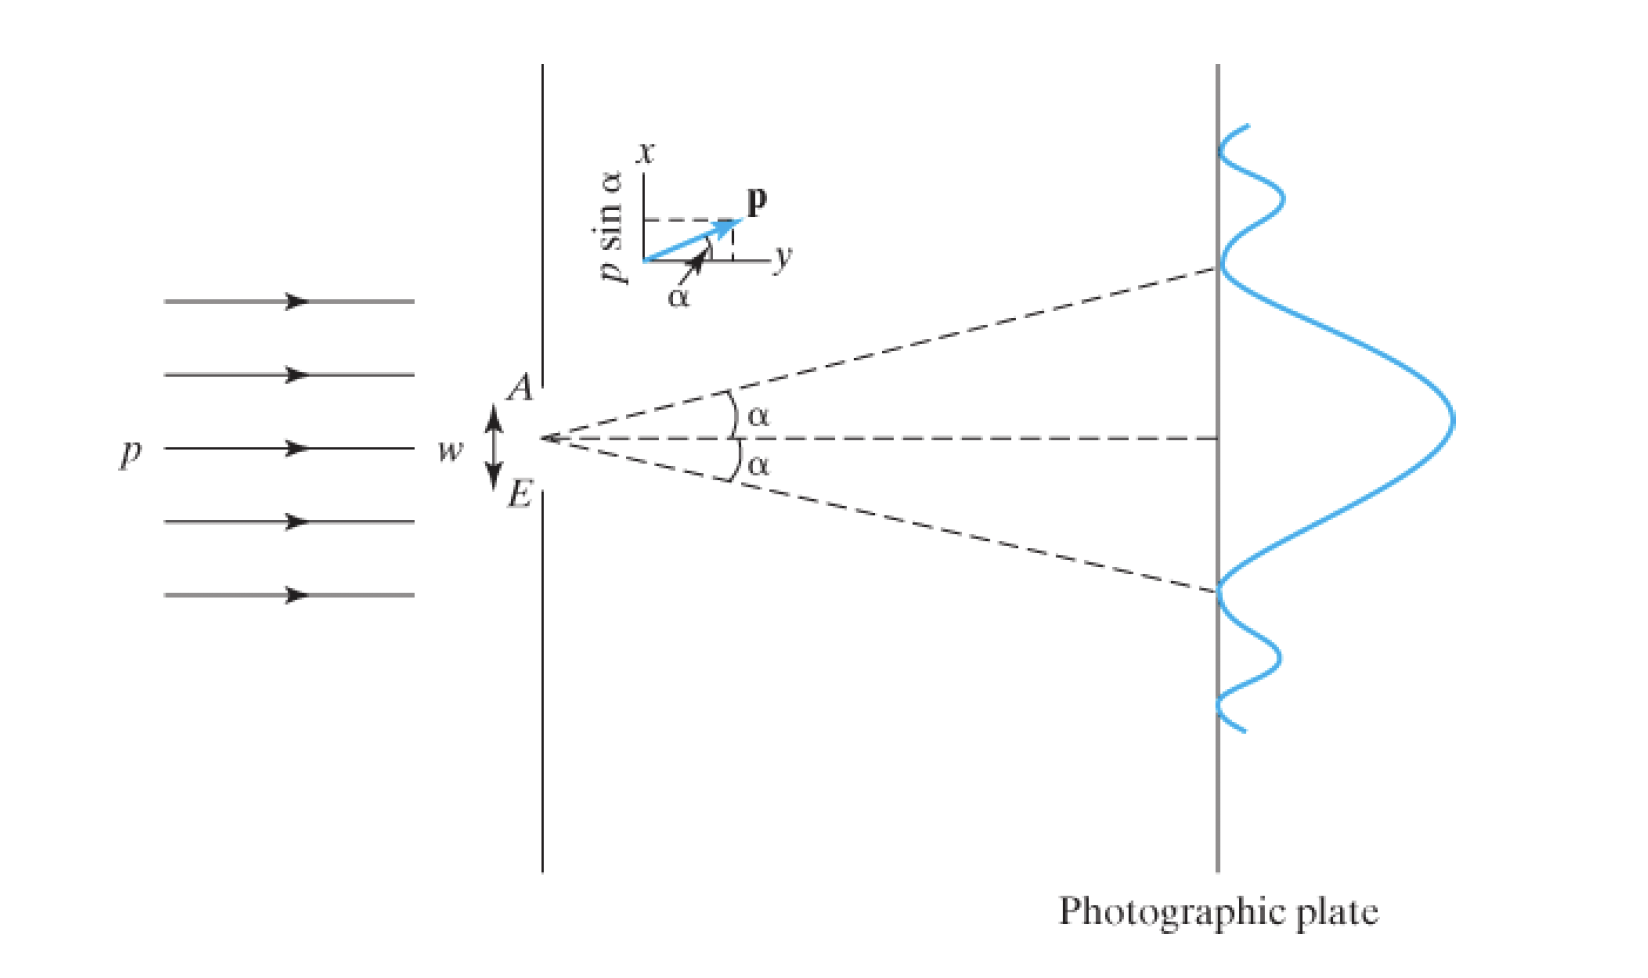
\includegraphics[width=0.8\textwidth]{/users/administrator/desktop/repo/quantumchemistry/Figures/1.1.png}  % 图片路径
		\caption{\text{狭缝的电子衍射}}
		\label{fig:1.1}
	\end{figure}
	\begin{figure}[h!]
		\centering
		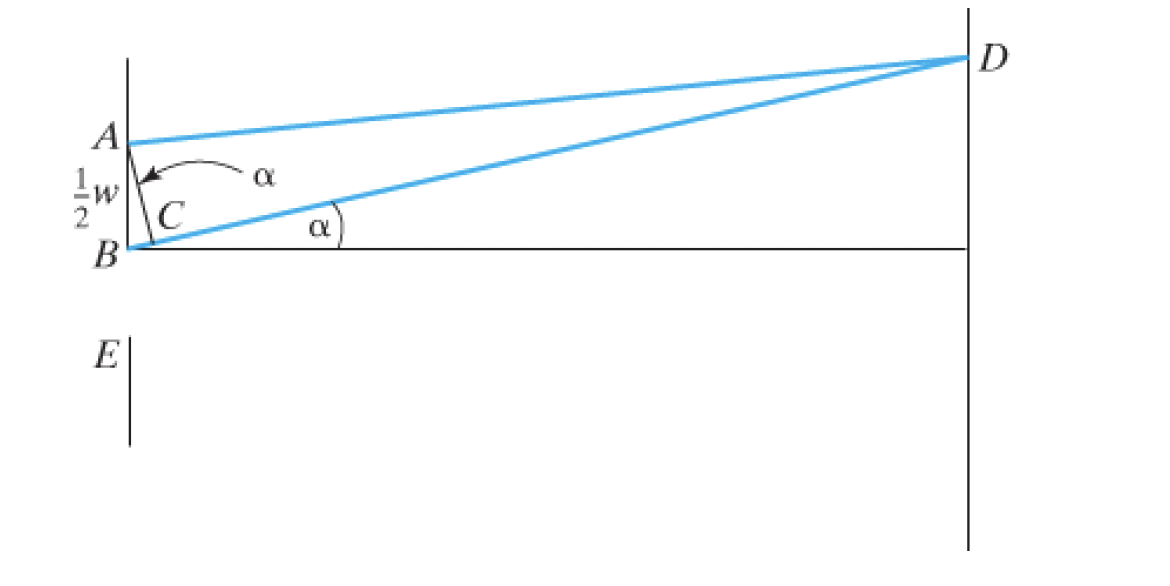
\includegraphics[width=0.6\textwidth]{/users/administrator/desktop/repo/quantumchemistry/Figures/1.2.png}
		\caption{\text{计算一级衍射的最小值}}
		\label{fig:1.2}
	\end{figure}
	
	\indent 第一个衍射最小值出现的角度$\alpha$很容易计算。出现第一个最小值的条件是:通过狭缝上边缘的粒子和通过狭缝中心的粒子所经过的距离之差应等于$\frac{1}{2}\lambda$,其中$\lambda$是相关波的波长。这样,从狭缝顶部发出的波与从狭缝中心发出的波正好相位相反,它们相互抵消。从狭缝中点以下距离$d$处发出的波与从狭缝顶部以下距离$d$处发出的波相互抵消。在图 \ref{fig:1.2}中画出$AC$,使 $AD=CD$,则路径长度之差为$BC$。狭缝到屏幕的距离比狭缝宽度大。因此,由于$AD$和$BD$几乎平行,则$\angle ACB$基本上是直角,因此$\angle BAC = \alpha$ ,路径差$BC$就是$\frac{1}{2}w \sin \alpha$。 设$BC$等于$\frac{1}{2}\lambda$,我们就得到了$w\sin\alpha=\lambda$,公式(\ref{eq:1.6 diffract equation on x}) 就变成了$\Delta x \Delta p_x=p\lambda$,其中波长$\lambda$由德布罗意关系式$\lambda=h/p$给出,因此$\Delta x \Delta p_x=h$。由于不确定度尚未精确定义,因此使用等号并不合适。我们可以用 
	\begin{equation}
		\Delta x \Delta p_x \approx h
		\label{eq:1.7 uncertinty on x}
	\end{equation}
	来表示$x$方向上的不确定性,同时$p_x$具有与普朗克常数相当的的数量级。\\
	\indent 尽管我们只用一种特例证明了(\ref{eq:1.7 uncertinty on x}),但其有效性是普遍的。无论如何尝试,微观 “粒子 ”的波粒二象性都限制了我们同时测量这种粒子的位置和动量的能力。我们对位置的测定越精确,对动量的测定就越不准确。(在图\ref{fig:1.1}中,$\sin \alpha = \lambda / w$,因此缩小狭缝会增加衍射图样的扩散)这种限制就是沃纳·海森堡(Werner Heisenberg)于 1927 年发现的\textbf{不确定性关系}。\\
	\indent 由于波粒二象性,测量行为会给被测系统带来不可控制的干扰。我们从粒子具有精确的$p_x$值(零)开始。通过施加狭缝,我们测量了粒子的$x$坐标,精确度为$w$,但这次测量给粒子的$p_x$值带来了不确定性。测量改变了系统的状态。
	
	
	\section{含时薛定谔方程}
	经典力学只适用于宏观粒子。对于微观 “粒子”,我们需要一种新的力学形式,即\textbf{量子力学}。为简单起见,我们将讨论一个单粒子的一维系统。\\
	\indent 在经典力学中,粒子的运动遵循牛顿第二定律:
	\begin{equation}
		\boxed{F = ma = m \frac{\text{d}^2x}{\text{d}t^2}}
		\label{eq:1.8 Newton's second law}
	\end{equation}
	其中$F$是作用在粒子上的合外力,$m$是粒子的质量,$t$是时间;$a$是加速度,由$a = \text{d} v / \text{d}t = \left(\text{d} / \text{d}t\right)\left(\text{d}x / \text{d}t\right) = \text{d}^2x / \text{d} t^2$给出,其中$v$是速度。方程(\ref{eq:1.8 Newton's second law})包含坐标$x$对时间的二阶导数。为了求解这个方程,我们必须进行两次积分。这就引入了两个积分常量$c_1$和$c_2$,有
	\begin{equation}
		x=g\left(t,c_1,c_2\right)
		\label{eq:1.9 function of the x-coordinate}
	\end{equation}
	其中$g$是时间的某个函数。我们现在要问:在某一特定时间$t_0$,我们必须掌握哪些信息才能预测粒子未来的运动?如果我们知道在$t_0$时刻,粒子位于$x_0$处,则有
	\begin{equation}
		x_0=g\left(t_0,c_1,c_2\right)
		\label{eq:1.10 initial function of the x-coordinate}
	\end{equation}
	由于我们需要确定两个常数,因此需要更多信息。将(\ref{eq:1.9 function of the x-coordinate})左右两边对时间求导,有
	\begin{equation*}
		\frac{\text{d} x }{\text{d}t} = v = \frac{\text{d}}{\text{d} t} g\left(t,c_1,c_2\right)
		\label{eq*:derivative of g function with respect to time}
	\end{equation*}
	如果我们也知道在$t_0$时刻,粒子具有速度$v_0$,那么有进一步的关系
	\begin{equation}
		v_0 = \eval{\frac{\mathrm{d}}{\mathrm{d} t} g(t, c_1, c_2)}_{t = t_0}
		\label{eq:1.11 v_0's equation}
	\end{equation}
	知道$x_0$和$v_0$后,我们可以用方程(\ref{eq:1.10 initial function of the x-coordinate})和(\ref{eq:1.11 v_0's equation})求出$c_1$和$c_2$。知道$c_1$和$c_2$后,就可以用方程(\ref{eq:1.9 function of the x-coordinate})来精确预测粒子在未来的运动。\\
	 \indent 作为式(\ref{eq:1.8 Newton's second law})至(\ref{eq:1.11 v_0's equation})的例子,考虑一个粒子在地球重力场中的运动。取垂直向上为$x$轴正方向,则作用在粒子上的合外力方向垂直向下,大小为$-mg$,其中$g$是重力加速度。则牛顿第二定律(\ref{eq:1.8 Newton's second law})形式为$-mg=m\mathrm{d}^2x/\mathrm{d}t^2$,所以$\mathrm{d}^2x/\mathrm{d}t^2=-g$。积分一次,有$\mathrm{d}x/\mathrm{d}t=-gt+c_1$。如果我们知道粒子在$t_0$时刻的速度为$v_0$,就可以求出积分常量$c_1$。又由于$v=\mathrm{d}x/\mathrm{d}t$,将$v_0=-gt_0+c_1$即$c_1=v_0+gt_0$带入,有$\mathrm{d}x/\mathrm{d}t=-gt+gt_0+v_0$。再次积分,我们引入了另一个积分常量$c_2$。如果我们知道粒子在$t_0$时刻的位置为$x_0$,则可以求出$c_2$。	因此,我们有$x=x_0-\frac{1}{2}g\left(t-t_0\right)^2+v_0\left(t-t_0\right)$。知道了在$t_0$时刻粒子的$x_0$和$v_0$,我们就能预测粒子未来的运动轨迹。\\
	 \indent 在一维范围内运动的粒子的经典力学势能$V$的定义为满足
	 \begin{equation}
	 	\boxed{\frac{\partial V \left(x,t\right)}{\partial x} = -F\left(x,t\right)}
	 	\label{eq:1.12 Potential energy in classical mechanics}
	 \end{equation}
	 例如,对于一个在地球重力场中运动的粒子,有$\partial V / \partial x = -F = mg$,积分一次,有$V = mgx+c$,其中$c$为积分常量。我们可以任意选择我们想要的零势能面。令$c=0$,我们有势能函数$V=mgx$。\\
	 \indent 经典力学中的 “\textbf{状态} ”一词是指系统中每个粒子在某一时刻的位置和速度,以及作用在粒子上的力。根据牛顿第二定律,给定一个系统在任何时候的状态,它的未来状态和未来运动都是完全确定的,如式(\ref{eq:1.9 function of the x-coordinate})-(\ref{eq:1.11 v_0's equation})所示。牛顿定律在解释行星运动方面取得的巨大成功让许多哲学家将牛顿定律作为哲学决定论的论据。数学家和天文学家拉普拉斯(Laplace)(1749-1827)假定宇宙是由服从牛顿定律的粒子组成的。因此,给定宇宙在某一时刻的状态,宇宙万物未来的运动是完全确定的。原则上,一个能知道宇宙任何瞬间状态的超级星体可以计算出所有未来的运动。
	% 小字号且缩进的段落
	\begin{quote}
		\small % 字号小一号(可选 \footnotesize 更小)
		\noindent % 取消首行缩进(可选)
		尽管经典力学是确定性的,但许多经典力学系统(例如,在重力、摩擦力和周期性变化的驱动力影响下摆动的摆)在系统参数的一定范围内表现出混沌行为。在混沌系统中,运动对粒子位置和速度的初始值以及作用力异常敏感,两个初始状态相差一个实验无法检测的量,最终会导致系统的未来行为大相径庭。因此,由于测量初始状态的精度有限,即使系统服从确定性方程,实际上也不可能预测混沌经典力学系统的长期行为。对太阳系行星数千万年轨道的计算机计算表明,行星的运动是混沌的。[I. Peterson, 《牛顿的钟:混沌的太阳系》,Freeman,1993 年;J. J. Lissauer,Rev. Mod. 71, 835 (1999)]
	\end{quote}
	\indent 
	\indent 只要精确了解经典力学系统的当前状态,我们就能预测其未来状态。然而,海森堡不确定性原理表明:我们无法同时确定微观粒子的精确位置和速度,因此无法获得经典力学所需的数据来预测系统的未来运动。 在量子力学中,我们必须满足于对未来精确运动的不完全预测。\\
	\indent 我们研究量子力学的方法是\textit{假设}基本原理,然后利用这些假设推导出实验可检验的结果,例如原子的能级。为了描述量子力学中一个系统的\textbf{状态},我们假设存在一个粒子坐标的函数$\Psi$,称为\textbf{状态函数}或\textbf{波 函数}(通常写作\textbf{波函数})。由于状态一般会随时间变化,因此$\Psi$也是时间的函数。对于一个单粒子的一维系统,我们有$\Psi=\Psi\left(x,t\right)$。波函数包含了一个系统所有可能的信息,因此我们不说 “波函数$\Psi$所描述的状态”,而只说 “状态$\Psi$”。 牛顿第二定律告诉我们,如何通过对经典力学系统当前状态的了解来找到它的未来状态。而要根据量子力学系统当前的状态找到它未来的状态,我们需要一个方程来告诉我们波函数是如何随时间变化的。对于单粒子的一维系统,将这个方程假定为
	\begin{equation}
		-\frac{\hbar}{\mathrm{i}}\frac{\partial \Psi \left(x,t\right)}{\partial t}= -\frac{\hbar^2}{2m}\frac{\partial^2 \Psi \left(x,t\right)}{\partial x^2}+ V\left(x,t\right)\Psi\left(x,t\right)
		\label{eq:1.13 Time-dependent Schödinger equation}
	\end{equation}
	其中常数$\hbar$(约化普朗克常数)定义为
	\begin{equation}
		\boxed{\hbar \equiv \frac{h}{2 \pi}}
		\label{eq:1.14 h-bar's definition}
	\end{equation}
	\indent 1926 年,奥地利物理学家埃尔温·薛定谔(Erwin Schrödinger)(1887-1961)建立了波函数的概念及其随时间变化的方程。这个被称为\textbf{含时薛定谔方程}(或\textbf{薛定谔波方程})中,$\mathrm{i}$是虚数单位,$m$是粒子的质量,$V\left(x,t\right)$是系统的势能函数。(量子力学中许多具有重要历史意义的论文可在 dieumsnh.qfb.umich.mx/archivoshistoricosmq 网站上查阅)\\
	\indent 含时薛定谔方程包含波函数对时间的一阶导数,如果我们知道$t_0$时刻的波函数,就可以计算出未来任意时刻的波函数(状态)。\\
	\indent 波函数包含了我们可能知道的关于它所描述的系统的所有信息。关于粒子$x$坐标的测量结果,$\Psi$给了我们什么信息?我们不能指望$\Psi$会像经典力学系统的状态那样具有涉及位置的明确说明。这个问题的正确答案是在薛定谔发现薛定谔方程后不久,由马克斯·玻恩(Max Born)给出的。玻恩推测:对于单粒子的一维系统,
	\begin{equation}
		\left|\Psi \left(x,t\right)\right|^2 \mathrm{d}x
		\label{exp:1.15 probability of a particle}
	\end{equation}
	给出了在$t$时刻,在$x$到$x+ \mathrm{d}x$范围内找到该粒子的概率。在(\ref{exp:1.15 probability of a particle})中,两条竖线表示绝对值,$\mathrm{d}x$表示$x$轴上一个无限小的长度。函数$\left|\Psi \left(x,t\right)\right|^2$是在$x$轴上不同位置找到粒子的\textbf{概率密度}。(第 1.6 节回顾了概率)例如,假设在某个特定时间$t_0$,粒子处于由波函数$a^2\mathrm{e}^{-2bx^2}$描述的特征状态,其中$a$和$b$是实常数。如果我们在$t_0$时刻观测该粒子的位置,会得到任意的$x$值,因为概率密度$a^2\mathrm{e}^{-2bx^2}$处处非零。由于$\left|\Psi\right|^2$在原点取到最大值,因此在$x=0$附近的$x$值比其他地方的更有可能被观测到。\\
	\indent 为了将$\Psi$与实验测量联系起来,我们需要许多完全相同的非相互作用系统,每个系统都处于相同的状态$\Psi$。如果我们对$n$个系统进行了$n$次测量,令$\mathrm{d}n_x$表示在$x$和$x+\mathrm{d}x$之间找到粒子的测量次数,那么$\mathrm{d}n_x/n$就是在$x$和$x+\mathrm{d}x$之间找到粒子的概率。因此,有
	\begin{equation*}
		\frac{\mathrm{d}n_x}{n} = \left|\Psi\right|^2\mathrm{d}x
	\end{equation*}
	而$\left(1/n\right) \mathrm{d}n_x / \mathrm{d}x$与$x$的关系图则给出了概率密度$\left|\Psi\right|^2$与$x$的函数关系。也许有人认为,我们可以通过一个处于$\Psi$状态的系统,反复测量粒子的位置来找到概率密度函数。这种方法是错误的,因为测量过程通常会改变系统的状态。我们在讨论不确定性原理(第 1.3 节)时看到过一个这方面的例子。\\
	\indent 量子力学是\textit{统计性质}的。在知道状态的情况下,我们无法准确预测位置测量的结果;我们只能预测各种可能结果的\textit{概率}。氢原子的玻尔理论规定了电子的精确路径,因此不是正确的量子力学图景。\\
	\indent 量子力学并没有说电子像波一样分布在空间的很大区域。相反,用于描述电子运动的概率模式(波函数)表现得像波,并满足波方程。\\
	\indent 波函数如何为我们提供位置以外的其他属性信息,将在后面的章节中讨论。\\
	\indent 热力学公设(热力学第一、第二和第三定律)是由宏观经验提出的,因此相当容易理解。量子力学的公设是从微观世界的角度阐述的,显得相当抽象。不要指望第一次接触就能完全理解量子力学公设。随着我们对各种实例的处理,对这些公设的理解会加深。\\
	\indent 我们引入了薛定谔方程,却没有试图证明它的合理性,这可能会让读者感到困惑。通过几何光学和经典力学之间的类比,以及波光学和量子力学之间的类比,我们可以证明薛定谔方程的合理性。几何光学是波光学的近似,在光的波长远小于仪器尺寸时有效。(回忆一下它在处理镜片和镜子时的用途)。同样地,经典力学是波动力学的近似,当粒子的波长远小于仪器的尺寸时有效。我们可以根据已知的几何光学方程和波光学方程之间的关系,猜测如何从经典力学中得到量子力学的正确方程。由于许多化学家对光学并不特别熟悉,因此省略了这些论证。无论如何,这些类比只能使薛定谔方程看起来\textit{可信}。它们不能用来\textit{推导}或\textit{证明}这个方程。薛定谔方程是理论的一个\textit{假设},要通过其预测与实验的一致性来检验。(关于薛定谔得出方程的推理细节,请参阅 Jammer,第 5.3 节。参考文献中的作者姓名用斜体标出)\\
	\indent 量子力学为微观粒子提供了运动规律。从实验上看,宏观物体遵从经典力学。因此,要使量子力学成为有效的理论,当我们从微观粒子过渡到宏观粒子时,量子力学应还原为经典力学。量子效应与德布罗意波长$\lambda=h/mv$有关。由于$h$非常小,宏观物体的德布罗意波长近似为零。因此,在极限$\lambda \rightarrow 0$中,我们期望含时薛定谔方程能够还原为牛顿第二定律。我们可以证明这一点(见问题 7.59)。\\
	\indent 狭义相对论与经典力学的关系也存在类似的情况。在以$c$为光速的极限$v/c \rightarrow 0$中,狭义相对论可还原为经典力学。我们将要发展的量子力学形式将是非相对论的。相对论与量子力学的完全融合尚未实现。\\
	\indent 从历史上看,量子力学是由海森堡、玻恩和乔丹(Jordan)于 1925 年首次使用矩阵提出的,比薛定谔于 1926 年使用微分方程提出的量子力学早几个月。薛定谔证明:海森堡公式(称为\textbf{矩阵力学})等同于薛定谔公式(称为\textbf{波动力学})。1926 年,狄拉克和乔丹分别独立地用一种称为\textit{变换理论}的抽象版本提出了量子力学,它是矩阵力学和波动力学的概括(见《狄拉克》)。1948 年,费曼设计出了量子力学的\textit{路径积分}公式 [R. P. Feynman, Rev. Mod. Phys., 20, 367 (1948); R. P. Feynman,Rev. Mod. Phys., 20, 367(1948); R. P. Feynman and A. R. Hibbs, Quantum Mechanics and Path Integrals, McGraw-Hill, 1965]。
	
	\section{定态薛定谔方程}
	含时薛定谔方程(\ref{eq:1.13 Time-dependent Schödinger equation}) 看上去很可怕。幸运的是,量子力学在化学中的许多应用都不使用这个方程。取而代之的是更简单的定态薛定谔方程。现在,我们从一维单粒子的含时薛定谔方程导出定态薛定谔方程。\\
	\indent 首先,我们只讨论一种特殊情况,即势能$V$不是时间的函数,而只取决于$x$。系统没有受到与时间相关的外力作用时会出现此情况。此时,含时薛定谔方程为
	\begin{equation}
		-\frac{\hbar}{\mathrm{i}}\frac{\partial \Psi \left(x,t\right)}{\partial t}= -\frac{\hbar^2}{2m}\frac{\partial^2 \Psi \left(x,t\right)}{\partial x^2}+ V\left(x,t\right)\Psi\left(x,t\right)
		\label{eq:1.16 Time-dependent Schödinger equation}
	\end{equation}
	将式(\ref{eq:1.16 Time-dependent Schödinger equation})的解假设为时间函数和坐标$x$函数的乘积:
	\begin{equation}
		\boxed{\Psi\left(x,t\right)=f\left(t\right)\psi\left(x\right)}
		\label{eq:1.17 product of x and t}
	\end{equation}
	大写的$\Psi$用来表示含时的波函数,而小写的$\psi$表示只与$x$坐标有关的因子。与 (\ref{eq:1.17 product of x and t})) 形式的波函数相对应的状态具有某些特性(稍后讨论),这些特性使它们极具吸引力。[并非 (\ref{eq:1.16 Time-dependent Schödinger equation}) 的所有解都具有 (\ref{eq:1.17 product of x and t}) 的形式;见证明 3.51。]取 (\ref{eq:1.17 product of x and t}) 的偏导数,我们有
	\begin{equation*}
		\frac{\partial \Psi\left(x,t\right)}{\partial t} = \frac{\mathrm{d} f\left(t\right)}{\mathrm{d}t} \psi\left(x\right), \quad \frac{\partial^2 \Psi \left(x,t\right)}{\partial x^2}= f\left(t\right) \frac{\mathrm{d}^2\psi\left(x\right)}{\mathrm{d}x^2}
	\end{equation*}
	带入(\ref{eq:1.16 Time-dependent Schödinger equation}),有
	\begin{equation*}
		-\frac{\hbar}{\mathrm{i}}\frac{\mathrm{d}f\left(t\right)}{\mathrm{d}t}\psi\left(x\right)=-\frac{\hbar^2}{2m}f\left(t\right)\frac{\mathrm{d}^2\psi\left(x\right)}{\mathrm{d}x^2}+V\left(x\right)f\left(t\right)\psi\left(x\right)
	\end{equation*}
	\begin{equation}
			-\frac{\hbar}{\mathrm{i}}\frac{1}{f\left(t\right)}\frac{\mathrm{d}f\left(t\right)}{\mathrm{d}t}=-\frac{\hbar^2}{2m}\frac{1}{\psi\left(x\right)}\frac{\mathrm{d}^2\psi\left(x\right)}{\mathrm{d}x^2}+V\left(x\right)
			\label{eq:1.18}
	\end{equation}
	此时方程左右两边同除$f\psi$。一般来说,我们希望 (\ref{eq:1.18}) 两边各相等的量是$x$和$t$的某个函数。然而,(\ref{eq:1.18}) 的右边不依赖于$t$,所以 (\ref{eq:1.18}) 两边相等的函数必须与$t$无关。我们称这个常数为$E$。\\
	\indent 令式(\ref{eq:1.18})的左边等于$E$,我们有
	\begin{equation*}
		\frac{\mathrm{d}f\left(t\right)}{\mathrm{d}t}=-\frac{\mathrm{i}E}{\hbar}\mathrm{d}t
	\end{equation*}
	左右对时间求积分,有
	\begin{equation*}
		\ln f\left(t\right)= - \mathrm{i}Et/\hbar+C
	\end{equation*}
	其中$C$是任意常数。因此,
	\begin{equation*}
		f\left(t\right)=\mathrm{e}^C\mathrm{e}^{-\mathrm{i}Et/\hbar}=A\mathrm{e}^{-\mathrm{i}Et/\hbar}
	\end{equation*}
	其中$A$是代替了$\mathrm{e}^C$的任意常数。由于$A$可以作为因子包含在与$f\left(t\right)$相乘的函数$\psi\left(x\right)$中,因此$A$可以从$f\left(t\right)$中略去。所以,
	\begin{equation*}
		f\left(t\right)=\mathrm{e}^{-\mathrm{i}Et/\hbar}
	\end{equation*}
	\indent 令(\ref{eq:1.18})的右边等于$E$,我们有
	\begin{equation}
		\boxed{-\frac{\hbar^2}{2m}\frac{\mathrm{d}^2\psi\left(x\right)}{\mathrm{d}x^2}+V\left(x\right)\psi\left(x\right)=E\psi\left(x\right)}
		\label{eq:1.19 time-independent Schrödinger Equation}
	\end{equation}
	方程(\ref{eq:1.19 time-independent Schrödinger Equation})就是质量为$m$的单粒子一维运动的\textbf{定态薛定谔方程}。	常数$E$有什么意义?由于$E$在(\ref{eq:1.19 time-independent Schrödinger Equation})中作为$\left[E-V\left(x\right)\right]$出现,$E$的维数与$V$相同,因此$E$具有能量的量纲。事实上,我们假设$E$就是系统的能量。(这是后一章将讨论的一个更普遍假设的特例)因此,在势能仅是$x$的函数的情况下,存在如下形式的波函数
	\begin{equation}
		\Psi\left(x,t\right)=\mathrm{e}^{-\mathrm{i}Et/\hbar}\psi\left(x\right)
		\label{eq:1.20}
	\end{equation}
	这些波函数对应于恒定能量$E$的状态。在接下来的几章中,我们将主要关注如何找到各种系统的方程(\ref{eq:1.19 time-independent Schrödinger Equation})的解。\\
	\indent 式(\ref{eq:1.20}) 中的波函数是复数函数,但在实验中可观测到的量是概率密度$\left|\Psi\left(x,t\right)\right|^2$。复数绝对值的平方由复数与其复共轭的乘积给出,复共轭则是在出现i的地方用 -i 代替 i (见第 1.7 节)。因此,
	\begin{equation}
		\boxed{\left|\Psi\right|^2=\Psi^{\ast}\Psi}
		\label{eq:1.21 square of Psi}
	\end{equation}
	其中,$\ast$号表示复共轭。对于波函数(\ref{eq:1.20}),有
	\begin{equation*}
		\begin{aligned}
			\left|\Psi\left(x,t\right)\right|^2 &=\left[\mathrm{e}^{-\mathrm{i}Et/\hbar}\psi\left(x\right)\right]^{\ast}\mathrm{e}^{-\mathrm{i}Et/\hbar}\psi\left(x\right)\\
			& = \mathrm{e}^{\mathrm{i}Et/\hbar}\psi^{\ast}\left(x\right)\mathrm{e}^{-\mathrm{i}Et/\hbar}\psi\left(x\right)\\
			& = \mathrm{e}^0\psi^{\ast}\left(x\right)\psi\left(x\right)=\psi^\ast\left(x\right)\psi\left(x\right)
		\end{aligned}
	\end{equation*}
	\begin{equation}
		\left|\Psi\left(x,t\right)\right|^2=\left|\psi\left(x\right)\right|^2
		\label{eq:1.22 Psi and psi}
	\end{equation}
	在推导(\ref{eq:1.22 Psi and psi})时,我们假设$E$是实数,即$E=E^{\ast}$。这将会在第7.2节给出证明。\\
	\indent 因此,对于 (\ref{eq:1.20}) 形式的状态,概率密度由$\left|\Psi\left(x\right)\right|^2$给出,且不随时间变化。这种状态称为\textbf{定态}。由于具有物理意义的量是$\left|\Psi\left(x,t\right)\right|^2$,而且对于定态有$\left|\Psi\left(x,t\right)\right|^2=\left|\psi\left(x\right)\right|^2$,函数$\psi\left(x\right)$通常被称为\textbf{波函数},尽管定态的完整波函数是$\psi\left(x\right)$与$\mathrm{e}^{-\mathrm{i}Et/\hbar}$的乘积。\textit{定态}一词不应误导读者,让他们以为处于定态的粒子就是静止的。确定的是概率密度$\left|\Psi\right|^2$,而不是粒子本身。\\
	\indent 我们将主要关注能量恒定的状态(定态),因此通常会处理定态薛定谔方程(\ref{eq:1.19 time-independent Schrödinger Equation})。为简单起见,我们将此方程称为 “薛定谔方程”。请注意,薛定谔方程包含两个未知数:允许的能量$E$和允许的波函数$ \psi$。为了求解这两个未知数,我们除了要求它满足 (\ref{eq:1.19 time-independent Schrödinger Equation}) 以外,还需要有额外的条件(称为边界条件)。边界条件决定了允许的能量,因为只有特定的$E$值才能满足边界条件。这一点在后面章节讨论具体例子时会更加清楚。
	
	\section{概率}
	概率在量子力学中起着基础性的作用。本节主要回顾数学中的概率。\\
	\indent 关于概率的正确定义一直存在很多争议。其中一个定义如下: 如果一个实验有$n$个同样可能的结果,其中$m$个结果有利于某个事件$A$的发生,那么$A$发生的概率就是$m/n$。请注意:这个定义是循环论证,因为它指定了同样可能的结果,而概率才是我们要定义的。它只是假设我们能够识别同样可能发生的结果。另一个定义是基于多次实际操作实验:假设我们进行了$N$次实验,在其中的$M$次实验中,事件$A$发生了。那么将$A$发生的概率定义为
	\begin{equation*}
		\lim\limits_{N \to \infty}\frac{M}{N}
	\end{equation*}
	因此,如果我们重复抛一枚硬币,随着次数的增加,正面的比例会逐渐接近$1/2$。\\
	\indent 例如,假设我们想知道从一副包含 13 张红心的 52 张标准牌中随机抽取一张牌时,抽到红心的概率。有 52 张牌,因此有 52 种同样可能的结果。有 13 张红心,因此抽出红心有 13 种可能的结果。所以,$m/n = 13/52 = 1/4 $。即抽到红心的概率为 $1/4$。\\
	\indent 有时我们会关心两个相关事件同时发生的概率。例如,我们可能会问从一副 52 张牌中抽出两张红心的概率,假设抽出第一张牌后我们不放回去。第一次抽牌有 52 种可能的结果,而每一种可能都对应 51 种可能的第二次抽牌。我们有 52 $\cdot$ 51种可能的结果。因为有 13 张红心,所以有 13$\cdot$12 种不同的方法抽出两张红心。期望概率为 $\left(13\cdot12\right)/\left(52\cdot51\right)=1/17$。这个计算说明了定理: 两个事件$A$和 $B$ 同时发生的概率是 $A$ 发生的概率乘以 $B$ 随后发生的条件概率(计算时假设 $A$ 发生)。因此,如果 $A$ 是第一次抽中红心的概率,那么 $A$ 的概率就是 $13/52$。如果第一次抽到红心,那么第二次抽到红心的概率是 $12/51$,因为牌中还有 12 张红心。那么抽到两张红心的概率是 $\left(13/52\right)\left(12/51\right)=1/17$,如前所述。\\
	\indent 在量子力学中,我们必须处理涉及连续变量(例如 $x$ 坐标)的概率。谈论在 $x=0.5000...$这样一个特定点上发现粒子的概率是没有多大意义的,因为 $x$ 轴上有无数个点,而对于我们进行的任何有限次数的测量来说,精确得到 $0.5000...$的概率都是微乎其微的。相反,我们谈论的是在 $x$ 轴上位于 $x$ 和 $x+\mathrm{d}x$ 之间的微小区间内找到粒子的概率,$\mathrm{d}x$ 是长度的一个无穷小量。这个概率自然与区间的长度 $\mathrm{d}x$ 成正比,并且会随着 $x$ 轴的不同区域而变化。因此,粒子在 $x$ 和 $x+\mathrm{d}x$ 之间被发现的概率等于 $g\left(x\right)\mathrm{d}x$,其中 $g\left(x\right)$ 是某个函数,表示概率在 $x$ 轴上的变化情况。函数 $g\left(x\right)$ 称为\textbf{概率密度},因为它是单位长度上的概率。由于概率是实数、非负数,因此 $g\left(x\right)$ 必须是一个处处非负的实函数。波函数 $\Psi$ 可以取负值和复值,不是概率密度。 因此,量子力学假设概率密度为 $\left|\Psi\right|^2$ [公式 (\ref{exp:1.15 probability of a particle}) ]。\\
	\indent 粒子位于空间的某个有限区域$a \le x \le b$的概率是多少?为了求出这个概率,我们将在位于$a$和 $b$ 之间的所有无限小区域中找到粒子的概率 $\left|\Psi\right|^2\mathrm{d}x$ 相加,这就是如下定积分的定义:
	\begin{equation}
		\boxed{\int_{a}^{b}\left|\Psi\right|^2 \mathrm{d}x = \text{Pr}\left(a \le x \le b\right)}
		\label{eq:1.23 int of probability}
	\end{equation}
	其中,Pr 表示概率。概率为1则代表必然性。由于粒子肯定位于 $x$ 轴上的某处,因此我们要求
	\begin{equation}
		\boxed{\int_{-\infty}^{\infty} \left|\Psi\right|^2 \mathrm{d}x = 1}
		\label{eq:1.24 the definition of nomalization}
	\end{equation}
	若波函数$\Psi$满足式(\ref{eq:1.24 the definition of nomalization}),则我们说$\Psi$是\textbf{归一化的}。对于定态波函数,有$\left|\Psi\right|^2 = \left|\psi\right|^2$且$\int_{-\infty}^{\infty} \left|\psi\right|^2 \mathrm{d}x = 1$。
	\begin{examplebox}
		\textbf{例题:}\\
		一个单粒子一维系统在$t=0$时刻满足$\Psi = a^{-1/2}\mathrm{e}^{-\left|x\right|/a}$,其中$a = 1.0000$ nm。在$t=0$时对粒子的位置进行一次测量。\\
		(a)求测量值介于 $x = 1.5000$ nm 和 $x = 1.5001$ nm 之间的概率;\\
		(b)求测量值介于 $x = 0$ nm 和 $x = 2$ nm之间的概率;\\
		(c)求证:$\Psi$是归一化的。\\
		\\
		(a)在这个极小的区间内,$x$只变化了$0.0001$ nm,而$\Psi$从$\mathrm{e}^{-1.5000}$ nm $^{-1/2} = 0.22313$ nm $^{-1/2}$到$\mathrm{e}^{-1.5001}$ nm $^{-1/2} = 0.22311$ nm $^{-1/2}$,所以$\Psi$在这个区间可以近似为常数,将这一区间视为无穷小区间是一个很好的近似方法。带入(\ref{exp:1.15 probability of a particle})给出的期望概率公式,有
		\begin{equation*}
			\begin{aligned}
				\left|\Psi\right|^2 \mathrm{d}x = a^{-1/2} \mathrm{e}^{-2\left|x\right|/a}\mathrm{d}x & = \left(1 \: \text{nm}\right)^{-1} \mathrm{e}^{-2\left(1.5 \: \text{nm}\right)/\left(1 \:\text{nm}\right)}\left(0.0001 \:\text{nm}\right)\\
				& = 4.979 \times 10^{-6}
			\end{aligned}
		\end{equation*}	
		(也可见证明1.14)\\
		(b)使用式(\ref{eq:1.23 int of probability})以及$x \ge 0$时$\left|x\right| = x$,有
		\begin{equation*}
			\begin{aligned}
				\text{Pr} \left(0 \le x \le 2 \: \text{nm}\right) & = \int_{0}^{2 \: \text{nm}}\left|\Psi\right|^2 \mathrm{d}x  = a^{-1} \int_{0}^{2 \: \text{nm}} \mathrm{e}^{-2x/a}\mathrm{d}x\\
				& = \eval{-\frac{1}{2}\mathrm{e}^{-2x/a}}_{0}^{2 \: \text{nm}} = -\frac{1}{2}\left(\mathrm{e}^{-4}-1\right) = 0.4908
			\end{aligned}
		\end{equation*}
		(c)使用$\int_{-\infty}^{\infty} f\left(x\right) \mathrm{d}x = \int_{-\infty}^{0} f \left(x\right) \mathrm{d}x+\int_{0}^{\infty} f\left(x\right) \mathrm{d}x$,以及$x \ge 0$时$\left|x\right| = x$和$x < 0$时$\left|x\right| = -x$,有
		\begin{equation*}
			\begin{aligned}
				\int_{-\infty}^{\infty} \left|\Psi\right|^2 \mathrm{d}x  & = a ^{-1}\int_{-\infty}^{0} \mathrm{e}^{2x/a}\mathrm{d}x + a^{-1}\int_{0}^{\infty} \mathrm{e}^{-2x/a}\mathrm{d}x\\
				& = a^{-1}\left(\eval{\frac{1}{2}a\mathrm{e}^{2x/a}}_{-\infty}^{0}\right) + a^{-1}\left(\eval{-\frac{1}{2}a\mathrm{e}^{-2x/a}}_{0}^{\infty}\right) = \frac{1}{2} + \frac{1}{2} = 1 
			\end{aligned}
		\end{equation*}
		得证。\\
		\\
		\noindent \textbf{练习:}\\
		对于一个测量时态函数为$\Psi = \left(32 a^3 /\pi \right)^{1/4} x \mathrm{e}^{-ax^2}$的系统(其中 $a = 1.0000 \: \text{nm}^{-2}$),求测量值在 $x = 1.2000$ nm 和 $1.2001$ nm 之间的概率。将区间视为无穷小区间。\\
		(\textit{答案:}0.0000258。)
	\end{examplebox}
	
	\section{复数}
	我们已经知道波函数可以是复数,所以我们来回顾一下复数的一些性质。\\
	\indent \textbf{复数}$z$具有如下的形式:
	\begin{equation}
		z = x+\mathrm{i}y, \quad \text{其中} \: \mathrm{i}  \equiv \sqrt{-1}
		\label{eq:1.25 definition of complex number}
	\end{equation}
	且$x$和$y$是\textbf{实数}(不涉及负数平方根的数),如果在(\ref{eq:1.25 definition of complex number})中$y=0$,则$z$是实数。如果$y \neq 0$,则$z$是\textbf{虚数}。如果$x=0$且$y \neq 0$,则$z$是\textbf{纯虚数}。例如:6.83是实数,$5.4-3\mathrm{i}$是虚数,而$0.60\mathrm{i}$是纯虚数。实数和纯虚数是复数的特例,在(\ref{eq:1.25 definition of complex number})中,$x$和$y$分别是$z$的实部和虚部,即$x = \mathrm{Re} \left(z\right)$;$y = \mathrm{Im}\left(z\right)$。\\
	\indent 复数可以代表\textbf{复平面}(图 \ref{fig:1.3})上的一个点,其中,$z$ 的实部绘制在横轴上,虚部绘制在纵轴上。这幅图显然提示我们定义两个表征复数 $z$ 的量:点 $z$ 与原点的距离 $r$ 称为 $z$ 的\textbf{绝对值}或模;点 $z$ 的半径矢量与正横轴所成的角度 $\theta$ 则称为 $z$ 的\textbf{相位}或辐角。我们有
	\begin{equation}
		\left|z\right| = r = \left(x^2+y^2\right)^{1/2}, \qquad \tan \theta = y/x
		\label{eq:1.26 definition of phase and absolute value}
	\end{equation}
	\begin{equation*}
		x = r \cos \theta, \qquad y = r \sin \theta
	\end{equation*}
	所以我们可以把$z = x+ \mathrm{i}y$写作
	\begin{equation}
		z = r \cos \theta + \mathrm{i} \sin \theta = r \mathrm{e}^{\mathrm{i} \theta}
		\label{eq:1.27 Triangular forms of complex numbers}
	\end{equation}	
	由欧拉公式带入。(见证明 4.3)
	\begin{equation}
		\boxed{\mathrm{e}^{\mathrm{i}\theta} = \cos \theta + \mathrm{i} \sin\theta}
		\label{eq:1.28 Euler's equation}
	\end{equation}
	以上方程中的$\theta$角均采用弧度制。\\
	\indent 如果$z = x + \mathrm{i}y$,则它的\textbf{复共轭}$z^{\ast}$定义为
	\begin{equation}
		z^{\ast} \equiv x - \mathrm{i}y = r \mathrm{e} ^{-\mathrm{i}\theta}
		\label{eq:1.29 definition of complexconjugate}
	\end{equation}
		\begin{figure}[h!]
		\centering
		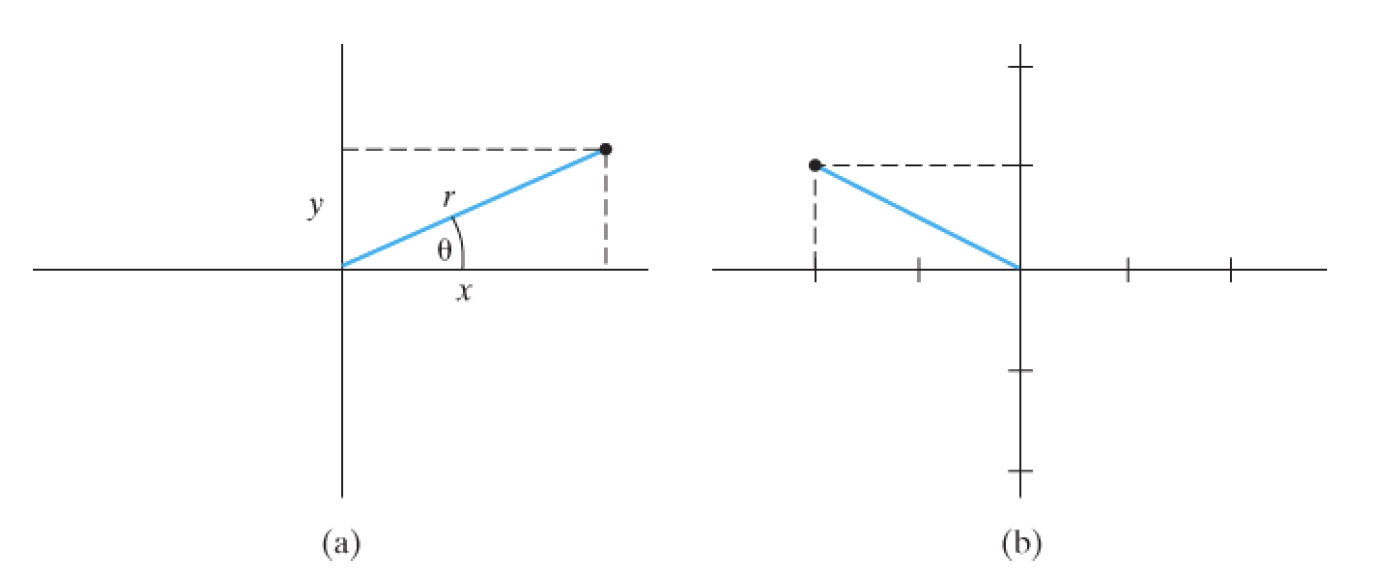
\includegraphics[width=0.8\textwidth]{/users/administrator/desktop/repo/quantumchemistry/Figures/1.3.png}  % 图片路径
		\caption{(a)\text{复数}$z = x + \mathrm{i}y$\text{的图象;}  (b)\text{复数}$-2+\mathrm{i}$\text{的图象}}
		\label{fig:1.3}
	\end{figure}\\
	\indent 如果$z$是实数,那么它的虚部为0。因此,当且仅当$z = z^{\ast}$时有$z$是实数。对复数$z$作两次复共轭,我们再次得到了$z$,所以$\left(z^{\ast}\right)^{\ast}=z$。将$z$与其复共轭$z^{\ast}$作乘积,我们有
	\begin{equation*}
		zz^{\ast} = \left(x + \mathrm{i}y\right)\left(x= \mathrm{i}y\right) = x^2+\mathrm{i}yx+\mathrm{i}xy-\mathrm{i}^2y^2
	\end{equation*}
	\begin{equation}
		\boxed{zz^{\ast} = x^2+y^2=r^2=\left|z\right|^2}
		\label{eq:1.30 product of z and its complex conjugate}
	\end{equation}
	对于两个复数$z_1=r_1\mathrm{e}^{\mathrm{i}\theta_1}$与$z_2 = r_2\mathrm{e}^{\mathrm{i}\theta_2}$的积和商,我们有
	\begin{equation}
		z_1z_2 = r_1r_2\mathrm{e}^{\mathrm{i}\left(\theta_1+\theta_2\right)}, \quad \frac{z_1}{z_2} = \frac{r_1}{r_2}\mathrm{e}^{\mathrm{i} \left(\theta_1 - \theta_2\right)}
		\label{eq:1.31 product and quotient of two complex numbers}
	\end{equation}
	\indent 根据复共轭的定义或 (\ref{eq:1.31 product and quotient of two complex numbers}),我们很容易证明
	\begin{equation}
		\boxed{\left(z_1z_2\right)^{\ast} = z_1^{\ast} z_2^{\ast}}
		\label{eq:1.32 properties of complex conjugate}
	\end{equation}
	同样地,
	\begin{equation}
		\boxed{
				\left(z_1/z_2\right) = z_1^{\ast} / z_2^{\ast}, \quad \left(z_1+z_2\right)^{\ast} = z_1^{\ast} + z_2^{\ast} , \quad \left(z_1-z_2\right)^{\ast} = z_1^{\ast} - z_2^{\ast}}
		\label{eq:1.33 linear properties of complex conjugate
		}
	\end{equation}
	对于积和商的绝对值,由(\ref{eq:1.31 product and quotient of two complex numbers})可知
	\begin{equation}
		\left|z_1z_2\right|=\left|z_1\right|\left|z_2\right|, \quad \left|\frac{z_1}{z_2}\right| = \frac{\left|z_1\right|}{\left|z_2\right|}
		\label{eq:1.34 properties of product and quotient absolute values}
	\end{equation}
	因此,如果$\psi$是复波函数,我们有
	\begin{equation}
		\left|\psi^2\right| = \left|\psi\right|^2 = \psi^{\ast} \psi
		\label{eq:1.35 properties of psi wave function}
	\end{equation}
	\indent 现在我们得到了数字 1 的 $n$ 次根式。我们可以将数字 1 的相位取为 0 或 $2\pi$ 或 $4\pi$,以此类推。因此 $1 = \mathrm{e}^{\mathrm{i}2\pi k}$,其中 $k$ 是任何整数,0、负数或正数。现在考虑数字 $\omega$,其中 $\omega \equiv \mathrm{e}^{\mathrm{i} 2\pi k /n}$,$n$ 为正整数。使用式(\ref{eq:1.31 product and quotient of two complex numbers}) $\:$$n$次,我们有$\omega^n = \mathrm{e}^{\mathrm{i}2\pi k} = 1$。因此,$\omega$是$n$次单位根。有 $n$ 个不同的复数 $n$ 次单位根,连续取 $n$ 个整数 $k$ 的值,就可以得到所有这些根:
	\begin{equation}
		\omega = \mathrm{e}^{\mathrm{i} 2\pi k /n}, \quad k = 0,1,2,\cdots , n-1
		\label{eq:1.36 n different complex nth roots of unity}
	\end{equation}
	除了 (\ref{eq:1.36 n different complex nth roots of unity}) 中的 $k$ 值之外,任何其他 $k$ 值所得到的数的相位都与 (\ref{eq:1.36 n different complex nth roots of unity}) 中的一个数相差 $2$ 的整数倍,因此不是不同的根。对于 (\ref{eq:1.36 n different complex nth roots of unity}) 中的 $n=2$,我们得到 1 的两个平方根;对于 $n=3$,得到 1 的三个立方根;以此类推。
	
	\section{单位}
	本书使用国际单位制。在国际单位制(SI)中,长度、质量、时间的单位分别是米(m)、千克(kg)和秒(s)。力的单位是牛顿(N),能量的单位是焦耳(J)。描述真空中相距 $r$ 的两个电荷 $Q_1$ 和 $Q_2$ 之间作用力大小的库仑定律,用国际单位制单位表示为
	\begin{equation}
		\boxed{F = \frac{Q_1Q_2}{4\pi \varepsilon_0r^2}}
		\label{eq:1.37 coulomb's law}
	\end{equation}
	其中电荷量$Q_1$和$Q_2$的单位是库仑(C),$\varepsilon_0$是常数(真空介电常数),其值为$8.854 \times 10^{-12} \mathrm{C}^2\mathrm{N}^{-1}\mathrm{m}^{-2}$。(物理常数的精确值见附录)
	
	\section{微积分学}
	量子化学中大量使用微积分,因此应牢记以下公式。其中 $c$、$n$ 和 $b$ 为常数,$f$ 和 $g$ 为 $x$ 的函数。
	\begin{equation*}
		\boxed{
			\frac{\mathrm{d}c}{\mathrm{d}x} = 0, \quad \frac{\mathrm{d}\left(cf\right)}{\mathrm{d}x} = c\frac{\mathrm{d}f}{\mathrm{d}x}, \quad \frac{\mathrm{d}x^n}{\mathrm{d}x} = nx^{n-1}, \quad \cfrac{\mathrm{d}\mathrm{e}^{cx}}{\mathrm{d}x} = c\mathrm{e}^{cx}
		}
	\end{equation*}
	\begin{equation*}
		\boxed{
			\frac{\mathrm{d}\left(\sin cx\right)}{\mathrm{d}x} = c \cos cx, \quad \frac{\mathrm{d} \left(\cos cx\right)}{\mathrm{d}x} = -c \sin cx, \quad \frac{\mathrm{d} \ln cx}{\mathrm{d} x } = \frac{1}{x}
		}
	\end{equation*}
	\begin{equation*}
		\boxed{
			\frac{\mathrm{d}\left(f+g\right)}{\mathrm{d}x} = \frac{\mathrm{d}f}{\mathrm{d}x}+\frac{\mathrm{d}g}{\mathrm{d}x}, \quad \frac{\mathrm{d}\left(fg\right)}{\mathrm{d}x} = f\frac{\mathrm{d}g}{\mathrm{d}x}+g\frac{\mathrm{d}f}{\mathrm{d}x}
		}
	\end{equation*}
	\begin{equation*}
		\boxed{
			\frac{\mathrm{d}\left(f/g\right)}{\mathrm{d}x} = \frac{\mathrm{d}\left(fg^{-1}\right)}{\mathrm{d}x} = -fg^{-2}\frac{\mathrm{d}g}{\mathrm{d}x}+g^{-1}\frac{\mathrm{d}f}{\mathrm{d}x}
		}
	\end{equation*}
	\begin{equation*}
		\boxed{
			\frac{\mathrm{d}}{\mathrm{d}x}f\left(g\left(x\right)\right) = \frac{\mathrm{d}f}{\mathrm{d}g}\frac{\mathrm{d}g}{\mathrm{d}x}
		}
	\end{equation*}
	最后一个公式有一个例子:$\mathrm{d}\left[\sin\left(cx^2\right)\right]/\mathrm{d}x = 2cx\cos\left(cx^2\right)$。这里$g\left(x\right) = cx^2$而$f=\sin$。
	\begin{equation*}
		\boxed{
			\int cf\left(x\right)\mathrm{d}x = c \int f\left(x\right)\mathrm{d}x, \quad \int \left[f\left(x\right)+g\left(x\right)\right]\mathrm{d}x = \int f\left(x\right)\mathrm{d}x+\int g\left(x\right)\mathrm{d}x
		}
	\end{equation*}
	\begin{equation*}
		\boxed{
			\int \mathrm{d}x = x, \quad \int x^n\mathrm{d}x = \frac{x^{n+1}}{n+1} \: \text{其中} \: n \neq -1, \quad \int \frac{1}{x}\mathrm{d}x = \ln x
		}
	\end{equation*}
	\begin{equation*}
		\boxed{
			\int \mathrm{e}^{cx}\mathrm{d}x = \frac{\mathrm{e}^{cx}}{c}, \quad \int \sin cx\mathrm{d}x = -\frac{\cos cx}{c}, \quad \int \cos cx\mathrm{d}x = \frac{\sin cx}{c}
		}
	\end{equation*}
	
	
	
	
	\section*{总结}

	\section*{习题}

	
	% ===== CHAPTER 2 =====
\chapter{箱中粒子}
	单粒子一维系统的定态波函数和能级是通过求解定态薛定谔方程 (\ref{eq:1.19 time-independent Schrödinger Equation}) 得到的。在本章中,我们将求解一个简单系统的定态薛定谔方程,即一维盒子中的粒子(第 2.2 节)。由于薛定谔方程是微分方程,我们首先讨论微分方程。
\section{微分方程}
	本节只讨论常微分方程,即只有一个自变量的方程。[偏微分方程有不止一个自变量。含时薛定谔方程 (\ref{eq:1.16 Time-dependent Schödinger equation}) 就是一个例子,其中 $t$ 和 $x$ 都是自变量。] 
	常微分方程是自变量 $x$、因变量$y\left(x\right)$和$y$的1、2、$\cdots$、$n$阶导数$y\left(y^{\prime},y^{\prime\prime}, \cdots, y^{\left(n\right)}\right)$之间的关系式。例如
	\begin{equation}
		y^{\prime\prime\prime}+2x\left(y^{\prime}\right)^2+y^2\sin x = 3\mathrm{e}^x
		\label{eq:2.1 an example of differential equation}
	\end{equation}
	微分方程的阶数与方程中最高阶导数的阶数相同。因此,方程 (\ref{eq:2.1 an example of differential equation}) 为三阶微分方程。\\
	\indent \textbf{线性微分方程}是一种特殊的微分方程,其形式为
	\begin{equation}
		A_n\left(x\right)y^{\left(n\right)}+A_{n-1}\left(x\right)y^{\left(n-1\right)}+A_{n-2}\left(x\right)y^{\left(n-2\right)}+\cdots+A_1\left(x\right)y^{\prime}+A_0\left(x\right)y=g\left(x\right)
		\label{eq:2.2 linear differential equation}
	\end{equation}
	其中所有的$A_i$和$g$ (有些可能为零)只是$x$的函数。在$n$阶线性微分方程(\ref{eq:2.2 linear differential equation})中,$y$及其各阶导数的次幂均为一次。不满足式(\ref{eq:2.2 linear differential equation})的微分方程为\textbf{非线性}微分方程。如果(\ref{eq:2.2 linear differential equation})中的$g\left(x\right)=0$,则线性微分方程是\textbf{齐次}的,否则是\textbf{非齐次}的。一维定态薛定谔方程(\ref{eq:1.19 time-independent Schrödinger Equation})就是二阶线性齐次微分方程。\\
	\indent 通过除以 $y^{\prime \prime}$ 的系数,我们可以将每一个二阶线性齐次微分方程化为以下形式
	\begin{equation}
		y^{\prime\prime}+P\left(x\right)y^{\prime}+Q\left(x\right)y=0
		\label{eq:2.3 linear homogeneous differential equation}
	\end{equation}
	设$y_1$和$y_2$是两个满足方程(\ref{eq:2.3 linear homogeneous differential equation})的独立函数。“独立”的意思是$y_2$并不是$y_1$的简单倍数。因此,线性齐次微分方程(\ref{eq:2.3 linear homogeneous differential equation})的通解为
	\begin{equation}
		y = c_1y_1+c_2y_2
		\label{eq:2.4 general solution of the li_{}near homogeneous differential equation}
	\end{equation}
	其中$c_1$和$c_2$是任意常数。将式(\ref{eq:2.4 general solution of the li_{}near homogeneous differential equation})带入(\ref{eq:2.3 linear homogeneous differential equation})的左边即可轻松证明:
	\begin{equation}
		\begin{aligned}
			c_1 & y_1^{\prime\prime}+c_2y_2^{\prime\prime}+P\left(x\right)c_1y_1^{\prime}+P\left(x\right)c_2y_2^{\prime}+Q\left(x\right)c_1y_1+Q\left(x\right)c_2y_2\\
			& = c_1\left[	y_1^{\prime\prime}+P\left(x\right)y_1^{\prime}+Q\left(x\right)y_1\right]+c_2\left[	y_2^{\prime\prime}+P\left(x\right)y_2^{\prime}+Q\left(x\right)y_2\right]\\
			& = c_1 \cdot 0 + c_2 \cdot 0 = 0
		\end{aligned}
		\label{eq:2.5}
	\end{equation}
	其中我们用到了$y_1$和$y_2$是方程(\ref{eq:2.3 linear homogeneous differential equation})的解。\\
	\indent $n$ 次微分方程的通解通常有 $n$ 个任意常数。为了确定这些常数,我们可能需要\textbf{定解条件},即规定 $y$ 或其各阶导数在某一点或多点的值的条件。例如:如果 $y$ 是固定在两点上的振动弦的位移,我们就知道 $y$ 在这两点上必须为零。\\
	\indent 一个重要的特例是二阶\textbf{常系数}线性齐次微分方程:
	\begin{equation}
		y^{\prime\prime}+py^{\prime}+qy=0
		\label{eq:2.6 constant coefficients in linear homogeneous second-order differential equation}
	\end{equation}
	其中$p$与$q$是常数。为了解这个方程(\ref{eq:2.6 constant coefficients in linear homogeneous second-order differential equation}),我们暂且假定解的形式是$y = \mathrm{e}^{sx}$。我们正在寻找一个导数与常数相乘会与原函数相互抵消的函数。指数函数在微分时会重复,因此是正确的选择。将其代入 (\ref{eq:2.6 constant coefficients in linear homogeneous second-order differential equation}) 即可得出
	\begin{equation*}
		s^2\mathrm{e}^{sx}+ps\mathrm{e}^{sx}+q\mathrm{e}^{sx}=0
	\end{equation*}
	\begin{equation}
		\boxed{
			s^2+ps+q=0
		}
		\label{eq:2.7 auxiliary equation}
	\end{equation}
	方程 (\ref{eq:2.7 auxiliary equation}) 称为\textbf{特征方程}。它是一个有两个根 $s_1$ 和 $s_2$ 的一元二次方程,只要 $s_1$ 和 $s_2$ 不相等,就能给出 (\ref{eq:2.6 constant coefficients in linear homogeneous second-order differential equation}) 的两个独立解。因此,(\ref{eq:2.6 constant coefficients in linear homogeneous second-order differential equation})的通解为
	\begin{equation}
		\boxed{
			y = c_1\mathrm{e}^{s_1x}+c_2\mathrm{e}^{s_2x}
		}
		\label{eq:2.8 general solution for 2.6}
	\end{equation}
	例如,对于方程$y^{\prime\prime}+6y^{\prime}-7y=0$,其特征方程为$s^2+6s-7=0$。解这个特征方程,有$s_1=1$,$s_2=-7$,所以通解为$y = c_1\mathrm{e}^{x}+c_2\mathrm{e}^{-7x}$。

\section{一维盒子中的粒子}
	本节求解一维盒子中粒子的定态薛定谔方程。我们所说的粒子是指受到势能函数作用的粒子,该势能函数沿 $x$ 轴的任何位置都为无穷大,只有长度为 $l$ 的线段除外,在该线段上势能为零。这样的系统在物理上似乎是不真实的,但这种模型可以成功地应用于某些共轭分子;见问题 2.17。我们把原点放在线段的左端(图 2.1)。
	\begin{figure}[h!]
		\centering
		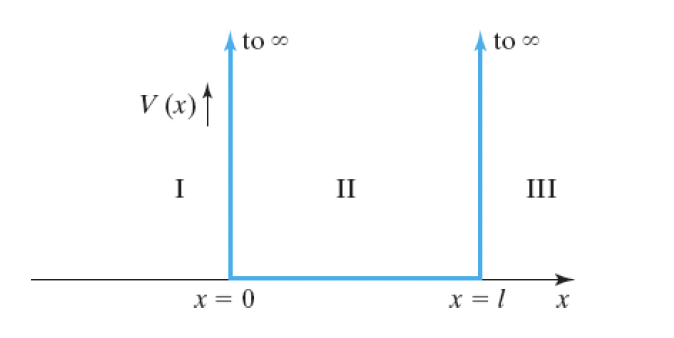
\includegraphics[width=0.6\textwidth]{/users/administrator/desktop/repo/quantumchemistry/Figures/2.1.png}  % 图片路径
		\caption{\text{一维盒子中粒子的势函数}$\: V\left(x\right)$}
		\label{fig:2.1}
	\end{figure}
	\\
	\indent 我们需要考虑三个区域。在区域I和III中,势能$V$为无穷大,此处的定态薛定谔方程(\ref{eq:1.19 time-independent Schrödinger Equation})为
	\begin{equation*}
		-\frac{\hbar^2}{2m}\frac{\mathrm{d}^2\psi}{\mathrm{d}x^2} = \left(E - \infty\right)\psi
	\end{equation*}
	与$\infty$相比,$E$的大小可以忽略不计。我们略去$E$,有
	\begin{equation*}
		\frac{\mathrm{d}^2\psi}{\mathrm{d}x^2} = \infty \psi, \quad \psi = \frac{1}{\infty}\frac{\mathrm{d}^2\psi}{\mathrm{d}x^2}
	\end{equation*}
	因此,在盒子的外侧,$\psi$为零:
	\begin{equation}
		\psi_I=0, \quad \psi_{II} = 0
		\label{eq:2.9 psi outside the box}
	\end{equation}
	\indent 对于区域II,$x$在0和$l$之间时,势能$V$为零,定态薛定谔方程(\ref{eq:1.19 time-independent Schrödinger Equation})为
	\begin{equation}
		\frac{\mathrm{d}^2\psi_{II}}{\mathrm{d}x^2}+\frac{2m}{\hbar^2}E\psi_{II}=0
		\label{eq:2.10 schrödinger equation for particle between 0 and l}
	\end{equation}
	其中$m$是粒子的质量,$E$是能量。我们将方程(\ref{eq:2.10 schrödinger equation for particle between 0 and l})视为一个二阶常系数线性齐次微分方程。其特征方程由(\ref{eq:2.7 auxiliary equation})给出:
	\begin{equation*}
		s^2 + 2mE\hbar^{-2}=0
	\end{equation*}
	\begin{equation}
		s = \pm \left(-2mE\right)^{1/2}\hbar^{-1}
		\label{eq:2.11}
	\end{equation}
	\begin{equation}
		s = \pm \mathrm{i}\left(2mE\right)^{1/2}\hbar^{-1}
		\label{eq:2.12}
	\end{equation}
	其中$\mathrm{i}$是虚数单位。使用(\ref{eq:2.8 general solution for 2.6}),我们有
	\begin{equation}
		\psi_{II} = c_1\mathrm{e}^{\mathrm{i} \left(2mE\right)^{1/2} x /\hbar}+c_2\mathrm{e}^{-\mathrm{i} \left(2mE\right)^{1/2} x /\hbar}
		\label{eq:2.13 general solution for particle between zero and l}
	\end{equation}
	我们姑且令
	\begin{equation*}
		\begin{aligned}
			\theta & \equiv \left(2mE\right)^{1/2} x /\hbar \\
			\psi_{II} & = c_1\mathrm{e}^{\mathrm{i}\theta}+c_1\mathrm{e}^{-\mathrm{i}\theta}
		\end{aligned}
	\end{equation*}
	由$\mathrm{e}^{\mathrm{i}\theta} = \cos\theta+\mathrm{i}\sin\theta$ $\left[\ref{eq:1.28 Euler's equation}\right]$以及
	\begin{equation}
		\boxed{
			\cos\left(-\theta\right) = \cos\theta \: \text{and} \: \sin\left(-\theta\right) = -\sin\theta
		}
		\label{eq:2.14 properties of sin and cos}
	\end{equation}
	我们有
	$\mathrm{e}^{-\mathrm{i}\theta} = \cos \left(-\theta\right)+\mathrm{i}\sin\left(-\theta\right)=\cos\theta-\mathrm{i}\sin\theta$
	。因此,
	\begin{equation*}
		\begin{aligned}
			\psi_{II} & =c_1\cos\theta+\mathrm{i}c_1\sin\theta+c_2\cos\theta-\mathrm{i}c_2\sin\theta \\
			& = \left(c_1+c_2\right)\cos\theta+\left(\mathrm{i}c_1-\mathrm{i}c_2\right)\sin\theta \\
			& = A \cos\theta + B\sin\theta 
		\end{aligned}	
	\end{equation*}
	其中,$A$和$B$是新的任意常数。则
	\begin{equation}
		\psi_{II}= A \cos\left[\hbar^{-1}\left(2mE\right)^{1/2}x\right]+B \sin\left[\hbar^{-1}\left(2mE\right)^{1/2}x\right]
		\label{eq:2.15 complete wave function of psi ii}
	\end{equation}
	\indent 现在通过定解条件,我们来求出$A$和$B$。假设波函数是连续的,也就是说,它的值不会突然跳变,这似乎是合理的(见图 3.4)。如果$\psi$在$x=0$处连续,那么有$\psi_I$和$\psi_{II}$在$x=0$处的极限相同:
	\begin{equation*}
		\begin{aligned}
			\lim\limits_{x \to 0}\psi_I & = \lim\limits_{x \to 0}\psi_{II} \\
			0 & = \lim\limits_{x \to 0}\left\{A \cos\left[\hbar^{-1}\left(2mE\right)^{1/2}x\right]+B \sin\left[\hbar^{-1}\left(2mE\right)^{1/2}x\right]\right\} \\
			0 & = A
		\end{aligned}
	\end{equation*}
	由于
	\begin{equation}
		\boxed{
			\sin 0 = 0, \quad \cos 0 =1
		}
		\label{eq:2.16 sin0 and cos0}
	\end{equation}
	将$A=0$带入(\ref{eq:2.15 complete wave function of psi ii}),有
	\begin{equation}
		\psi_{II} = B\sin\left[\left(2\pi/h\right)\left(2mE\right)^{1/2}x\right]
		\label{eq:2.17 }
	\end{equation}
	又由函数在$x=l$处连续,我们有
	\begin{equation}
		B\sin\left[\left(2\pi/h\right)\left(2mE\right)^{1/2}l\right]=0
		\label{eq:2.18}
	\end{equation}
	因为我们不能令波函数处处为零-得到一个空箱子,所以$B$不能为零。有
	\begin{equation*}
		\sin\left[\left(2\pi/h\right)\left(2mE\right)^{1/2}l\right]=0
	\end{equation*}
	$\sin$函数的零点位于$0, \pm \pi, \pm 2\pi, \cdots, \pm n \pi$。则
	\begin{equation}
		\left(2\pi/h\right)\left(2mE\right)^{1/2}l = \pm n \pi
		\label{eq:2.19 introduction of n}
	\end{equation}
	\indent $n=0$是一种特殊情况。由(\ref{eq:2.19 introduction of n}),$n=0$意味着$E=0$。若$E=0$则特征方程(\ref{eq:2.12})有两个相等的根,且式(\ref{eq:2.13 general solution for particle between zero and l})不是薛定谔方程的完全解。为了找到完全解,我们回到(\ref{eq:2.10 schrödinger equation for particle between 0 and l}),其中$E=0$有$frac{\mathrm{d}^2\psi_{II}}{\mathrm{d}x^2}=0$。积分一次,有$\mathrm{d}\psi_{II}/\mathrm{d}x = c$;再积分一次,有$\psi_{II}=cx+d$,其中$c$和$d$都是常数。由于$x=0$时有$\psi_{II}=0$,所以$d=0$;又由于$x=l$时也有$\psi_{II}=0$,所以$c=0$。因此,$\psi_{II}=0$推出$E=0$,则$E=0$不是允许的能量值。即$n=0$是不允许的。\\
	\indent 从方程(\ref{eq:2.19 introduction of n})中解出$E$,我们有
	\begin{equation}
		\boxed{
			E = \frac{n^2h^2}{8ml^2}, \quad n = 1,2,3 \cdots
		}
		\label{eq:2.20 energy of one-dimensional box}
	\end{equation}
	\indent 只有能量值满足式(\ref{eq:2.20 energy of one-dimensional box})的波函数$\psi$,才能符合在$x=l$处连续的定解条件。定解条件的应用迫使我们得出能量值是量子化的结论(图 2.2)。这与经典结果形成了鲜明对比,经典结果认为盒子中的粒子可以具有任何非负能量。请注意:粒子的能量有一个大于零的最小值。能量最小的状态称为\textbf{基态}。能量高于基态能量的状态为\textbf{激发态}。(在经典力学中,粒子在盒子中的最低能量为零。经典粒子在盒内静止不动时,动能为零,势能为零)。
	\begin{figure}[h!]
		\centering
		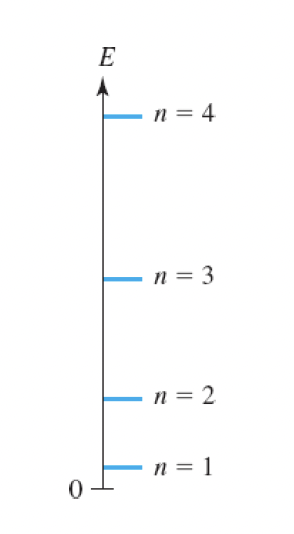
\includegraphics[width=0.2\textwidth]{/users/administrator/desktop/repo/quantumchemistry/Figures/2.2.png}  % 图片路径
		\caption{\text{一维盒子中粒子能量最低的四个能级}}
		\label{fig:2.2}
	\end{figure}
	\\
	\textbf{例题:}\\
	有一质量为$2.00\times10^{-26}\: \mathrm{g}$的粒子在长度$4.00 \: \mathrm{nm}$的势箱中运动。求该粒子从 $n=3$ 能级进入 $n=2$ 能级时发射光子的频率和波长。\\
	\indent 根据能量守恒,发射光子的能量等于两个定态之间的能量差[公式 (\ref{eq:1.4 Higher state to lower state delta energy}) ;另见第 9.9 节 ]:
	\begin{equation*}
		h\nu = E_{upper}-E_{lower}=\frac{n_u^2h^2}{8ml^2} - \frac{n_l^2h^2}{8ml^2}
	\end{equation*}
	\begin{equation*}
		\nu = \frac{\left(n_u^2-n_l^2\right)h}{8ml^2} = \frac{\left(3^2-2^2\right)\left(6.626 \times 10^{-34} \: \mathrm{J}\cdot\mathrm{s}\right)}{8\left(2.00 \times 10^{-29} \:  \mathrm{kg}\right)\left(4.00 \times 10^{-9} \: \mathrm{m}\right)^2} = 1.29 \times 10^{12} \: \mathrm{s}^{-1}
	\end{equation*}
	其中$u$和$l$分别代表高能级和低能级。由$\lambda \nu =c$,有$\lambda = 2.32 \times 10^{-4} \: \mathrm{m}$。(学生常见的错误是将 $h\nu$ 设为其中一个状态的能量,而不是状态间的能量\textit{差})\\
	\textbf{练习:}\\
	对于某个在一维盒子中运动的电子,其能级跃迁的最长波长为400 nm。求盒子的长度。\\
	\textit{答案:}0.603 nm\\
	
	\indent 将(\ref{eq:2.19 introduction of n})带入(\ref{eq:2.17 }),解出波函数为
	\begin{equation}
		\psi_{II} = B\sin\left(\frac{n\pi x}{l}\right), \quad n = 1,2,3\cdots
		\label{eq:2.21 wavefunction solution of psi ii with b}
	\end{equation}
	在 $n\pi$ 前面使用负号并不能得到另一个独立的解。因为 $\sin\left(-\theta\right)=-\sin\theta$,我们只会得到一个常数 -1,乘以带正号的解。\\
	\indent 公式 (\ref{eq:2.21 wavefunction solution of psi ii with b}) 中的常数 $B$ 仍然是任意的。为了将其确定下来,我们使用公式 (\ref{eq:1.24 the definition of nomalization}) 和 (\ref{eq:1.22 Psi and psi}) 对$\psi_{II}$进行归一化:
	\begin{equation*}
		\int_{-\infty}^{\infty}\left|\Psi\right|^2\mathrm{d}x = \int_{-\infty}^{\infty}\left|\psi\right|^2\mathrm{d}x = 1
	\end{equation*}
	\begin{equation*}
		\int_{-\infty}^{0}\left|\psi_I\right|^2\mathrm{d}x + \int_{0}^{l}\left|\psi_{II}\right|^2\mathrm{d}x +\int_{l}^{\infty}\left|\psi_{III}\right|^2\mathrm{d}x =1
	\end{equation*}
	\begin{equation}
		\left|B\right|^2\int_{0}^{l}\sin^2\left(\frac{n\pi x}{l}\right)\mathrm{d}x=1=\left|B\right|^2\frac{l}{2}
		\label{eq:2.22 process of fix constant B}
	\end{equation}
	其中的积分是用附录中的公式 (A.2) 求得的。我们有
	\begin{equation*}
		\left|B\right|^2=\left(2/l\right)^{1/2}
	\end{equation*}
	\indent 注意我们只求出了$B$的绝对值,但$B$可以取$\pm \left( 2/l\right) ^{1/2}$。此外,$B$也不必是实数,我们可以取任何模为$\left(2/l\right)^{1/2}$的复数。所以,我们可以说$B=\left( 2/l\right) ^{1/2}\mathrm{e}^{\mathrm{i}\alpha}$,其中$\alpha$是$B$的辐角,可以取0到$2\pi$之间的任何值(第 1.7 节)。取辐角为0,则箱中粒子的定态波函数为
	\begin{equation}
		\boxed{
			\psi_{II} = \left(\frac{2}{l}\right)^{1/2}\sin\left(\frac{n\pi x}{l}\right), \quad n = 1,2,3\cdots
		}
		\label{eq:2.23 stationary state wave function for the particle in a box}
	\end{equation}
	波函数和概率密度的图如图 \ref{fig:2.3} 和 \ref{fig:2.4} 所示。\\
	\indent 能量(\ref{eq:2.20 energy of one-dimensional box})和波函数(\ref{eq:2.23 stationary state wave function for the particle in a box})中的数字 $n$ 称为\textbf{量子数}。量子数 $n$ 的每个不同值都会产生不同的波函数和不同的状态。\\
	\indent 波函数在某些点为零,这些点被称为\textbf{节点}。量子数$n$每增加1,波函数$\psi$就多一个节点。$\psi$和$\left| \psi \right| ^2$ 中节点的存在似乎令人惊讶。因此,图(\ref{fig:2.4})表明:对于$n=2$,在箱的中点$x=2/l$处找到粒子的概率为零。粒子怎么可能从盒子的一侧运动到另一侧,而在任何时候都不会出现在盒子的中心呢?这个明显的悖论产生于我们试图用宏观粒子运动的日常经验来理解微观粒子的运动。然而,正如第 1 章所指出的:电子和其他微观 “粒子 ”无法用宏观世界的经典物理学概念来完整、正确地描述。\\
	\indent 图 \ref{fig:2.4} 显示,在盒子的不同位置找到粒子的概率与经典结果截然不同。从经典角度看,一个固定能量的粒子在盒子中以恒定的速度在两壁之间弹性地来回弹跳。因此,在盒子中的任何一点发现它的可能性都是相同的;从量子力学角度看,我们会发现在盒子中心的最低能级出现概率最大。随着能级越来越高,节点越来越多,概率的最大值和最小值就会越来越接近,而沿着盒子长度方向的概率变化最终会变得难以察觉。当量子数非常大时,我们就获得了接近于经典的均匀概率密度结果。
	\begin{figure}
		\centering
		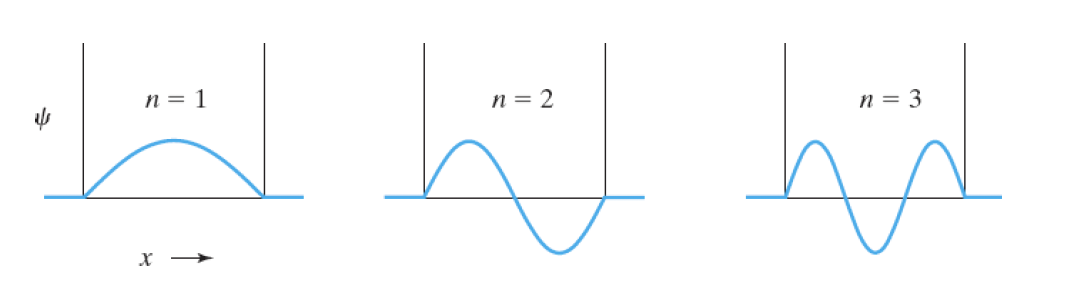
\includegraphics[width=0.8\textwidth]{/users/administrator/desktop/repo/quantumchemistry/Figures/2.3.png}  % 图片路径
		\caption{\text{三种能量最低的盒中粒子状态的} $\psi$ \text{曲线图}}
		\label{fig:2.3}
	\end{figure}
	\begin{figure}
		\centering
		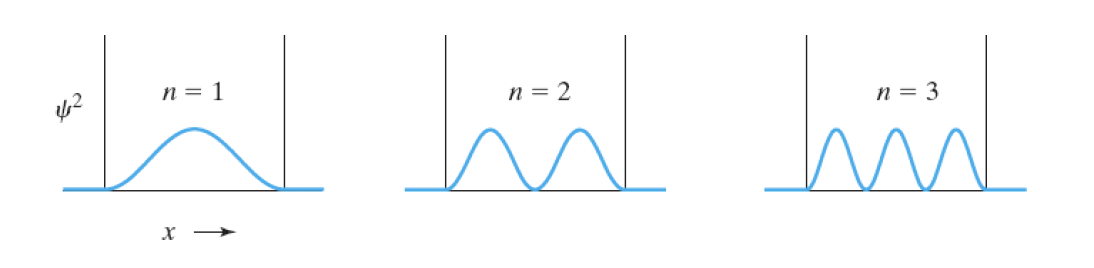
\includegraphics[width=0.8\textwidth]{/users/administrator/desktop/repo/quantumchemistry/Figures/2.4.png}  % 图片路径
		\caption{{三种能量最低的盒中粒子状态的} $\left| \psi \right| ^2$ \text{曲线图}}
		\label{fig:2.4}
	\end{figure}
	\indent 这一结果,即在大量子数极限下量子力学与经典力学的关系,被称为\textit{玻尔对应原理}。由于牛顿力学适用于宏观物体(运动速度远小于光速),我们期望非相对论量子力学能给出与经典力学对宏观物体相同的答案。由于普朗克常数极其微小,能量的量子化对于宏观物体来说是不可观测的。由于粒子的质量和盒子长度的平方出现在式 (\ref{eq:2.20 energy of one-dimensional box}) 的分母中,因此在宏观盒子中具有宏观运动能量的宏观物体将具有巨大的 $n$ 值,那么根据对应原理,宏观物体将显示出经典行为。\\
	\indent 现在,我们有了一整套波函数,每个波函数对应不同的能量,并以量子数 $n$(正整数)为特征。让下标 $i$ 表示量子数为 $n_i$ 的特定波函数:
	\begin{equation*}
			\psi_i = \left(\frac{2}{l}\right)^{1/2} \sin\left(\frac{n_i\pi x}{l}\right), \quad  0<x<l
	\end{equation*}
	\begin{equation*}
		\psi_i = 0, \quad  \text{其他区域}
	\end{equation*}
	由于波函数已归一化,我们有
	\begin{equation}
		\int_{-\infty}^{\infty}\psi_i^{\ast} \psi_j \mathrm{d}x = 1, \quad \text{若}i=j
		\label{eq:2.24}
	\end{equation}
	现在我们想知道,当我们使用对应于不同能级的波函数时,这个积分的值是多少:
	\begin{equation*}
		\int_{-\infty}^{\infty}\psi_i^{\ast} \psi_j \mathrm{d}x = \int_{0}^{l}\left(\frac{2}{l}\right)^{1/2}\sin\left(\frac{n_i\pi x}{l}\right)\left(\frac{2}{l}\right)^{1/2}\sin\left(\frac{n_j\pi x}{l}\right)\mathrm{d}x, \quad n_i \neq n_j
	\end{equation*}
	使用附录中的公式(A.5),我们有
	\begin{equation}
		\int_{-\infty}^{\infty}\psi_i^{\ast} \psi_j \mathrm{d}x = \frac{2}{l}\left[
			\frac{\sin \left[\left(n_i-n_j\right)\pi\right]}{2\left(n_i-n_j\right)\pi /l}- \frac{\sin \left[\left(n_i+n_j\right)\pi\right]}{2\left(n_i+n_j\right)\pi /l}
		\right] = 0
		\label{eq:2.25}
	\end{equation}
	由于当$m$是整数时有$\sin m \pi = 0$,则
	\begin{equation}
		\int_{-\infty}^{\infty}\psi_i^{\ast} \psi_j \mathrm{d}x = 0, \quad i \neq j
		\label{eq:2.26 definition of orthogonal wave functions}
	\end{equation}
	当(\ref{eq:2.26 definition of orthogonal wave functions})成立时,我们说对$i \neq j$的波函数$\psi_i$和$\psi_j$是互相\textbf{正交}的。将(\ref{eq:2.24})与(\ref{eq:2.26 definition of orthogonal wave functions})相结合,我们有
	\begin{equation}
		\int_{-\infty}^{\infty}\psi_i^{\ast} \psi_j \mathrm{d}x = \delta_{ij}
		\label{eq:2.27 orthogonal with kronecker delta}
	\end{equation}
	其中$\delta_{ij}$是\textbf{Kronecker符号}(由数学家的名字命名)。当$ $i 和 $j$ 相等时,它等于 1;当 $i$ 和 $j$ 不相等时,它等于 0:
	\begin{equation}
		\boxed{
			\delta_{ij} \equiv \begin{cases}
				0, \quad & i \neq j; \\
				1, \quad & i = j.
			\end{cases}
		}
		\label{eq:2.28 definition of kronecker delta}
	\end{equation}
	波函数的特性 (\ref{eq:2.27 orthogonal with kronecker delta})) 称为\textbf{正交归一性}。我们只证明了粒子盒内波函数的正交归一性。我们将在第 7.2 节更广泛地证明它。\\
	\indent 您可能会对式 (\ref{eq:2.26 definition of orthogonal wave functions}) 感到困惑,不明白为什么我们要将一个状态的波函数乘以另一个状态的波函数。我们稍后会看到(例如第 7.3 节),使用包含一个系统所有波函数之和的方程通常很有帮助,而这样的方程会导致像 (\ref{eq:2.26 definition of orthogonal wave functions}) 这样的积分。\\
	\indent 研究无限深势阱中粒子的一个更严谨的方法是:首先处理粒子在壁箱中的势能有限跃迁,然后当 $V$ 的跃迁变得无限大时求取极限。取极限时的结果与 (\ref{eq:2.20 energy of one-dimensional box}) 和 (\ref{eq:2.23 stationary state wave function for the particle in a box}) 相同(见问题 2.22)。\\
	\indent 我们只考虑了粒子在一维盒子中的定态。该系统的非稳态示例,请参见第 7.8 节末尾的示例。\\
	\indent 关于粒子在盒子中的在线计算机模拟,请访问 www.chem.uci.edu/undergraduate/applets/dwell/\\dwell.htm(显示了在盒子中间引入高度和宽度可变的屏障时对波函数和能级的影响);web. williams.\\edu/wpetc/chemistry/dbingemann/Chem153/particle.html(通过绘制薛定谔方程在能量变化和盒子长度变化时的解来显示量子化);以及 falstad.com/qm1d/(同时显示含时薛定谔方程和定态薛定谔方程;见 7.47)。

\section{一维自由粒子}
	我们所说的自由粒子是指不受任何力作用的粒子。对于自由粒子,对(\ref{eq:1.12 Potential energy in classical mechanics})的积分表明,无论 $x$ 的值是多少,势能都保持不变。由于基态能量的选择是任意的,我们可以设定 $V(x) = 0$。则薛定谔方程 (\ref{eq:1.19 time-independent Schrödinger Equation}) 变为
	\begin{equation}
		\frac{\mathrm{d}^2\psi}{\mathrm{d}x^2}+\frac{2m}{\hbar}E\psi = 0
		\label{eq:2.29 schrödinger equation for free particle}
	\end{equation}
	式 (\ref{eq:2.29 schrödinger equation for free particle}) 与式 (\ref{eq:2.10 schrödinger equation for particle between 0 and l}) 相同(定解条件除外)。因此, (\ref{eq:2.29 schrödinger equation for free particle}) 的通解为 (\ref{eq:2.13 general solution for particle between zero and l}) :
	\begin{equation}
		\psi = c_1\mathrm{e}^{\mathrm{i} \left(2mE\right)^{1/2} x /\hbar}+c_2\mathrm{e}^{-\mathrm{i} \left(2mE\right)^{1/2} x /\hbar}
		\label{eq:2.30}
	\end{equation}
	\indent 我们可以使用什么边界条件呢?似乎可以合理地假设(因为 $\psi^{\ast}\psi\mathrm{d}x$ 代表一种概率),当 $x$ 趋于 $\pm \infty$ 时,$\psi$ 将保持有限值。那么如果能量 $E$ 小于零,那么就违反了这个边界条件,因为对于 $E<0$,我们有
	\begin{equation*}
		\mathrm{i} \left(2mE\right)^{1/2} = \mathrm{i}\left(-2m \left|E\right|\right)^{1/2} = \mathrm{i} \cdot \mathrm{i} \cdot \left(2m \left|E\right|\right)^{1/2} = -\left(2m \left|E\right|\right)^{1/2}
	\end{equation*}
	因此,当 $x$ 接近负无穷大时,(\ref{eq:2.30})中的第一项将变为无穷大。同样,如果 $E$ 为负值,当 $x$ 接近正无穷大时,(\ref{eq:2.30}) 中的第二项也将变为无穷大。因此,对于一维自由粒子,定解条件要求
	\begin{equation}
		E \ge 0
		\label{neq: boundary condition of free particle}
	\end{equation}
	波函数是振荡的,是一个正弦项和一个余弦项的线性组合[公式 (\ref{eq:2.15 complete wave function of psi ii}) ]。对于自由粒子,能量没有量子化,所有非负能量都是允许的。在这种情况下,由于我们规定$V=0$,能量 $E$ 全为动能。如果我们想通过归一化的方式求出常数$c_1$和$c_2$,会发现积分$\int_{- \infty}^{\infty} \psi^{\ast}\left(x\right)\psi\left(x\right) \mathrm{d}x$的值为无穷大。换句话说,自由粒子的波函数在通常意义上是不可归一化的。这在物理上是意料之中的,因为当 $x$ 变为 $\pm \infty$  时,找到自由粒子的概率没有理由趋近于零。\\
	\indent 自由粒子问题是一种不真实的情况,因为我们实际上不可能有一种粒子与宇宙中的任何其他粒子没有相互作用。
	
	
	
	
	

\section{矩形势阱中的粒子}

\section{隧穿}

\section*{总结}

\section*{习题}

	
	% ===== CHAPTER 3 =====
\chapter{算符}
\label{chap:3}
\section{算符}
	\label{sec:3.1 Operators}
	现在,我们以一种比以前更一般的方式来发展量子力学理论。首先,我们将单粒子一维定态薛定谔方程 (\ref{eq:1.19 time-independent Schrödinger Equation}) 写成以下形式
	\begin{equation}
		\left[-\frac{\hbar^2}{2m}\frac{\mathrm{d}^2\psi}{\mathrm{d}x^2}+V\left(x\right)\right]\psi\left(x\right) = E\psi\left(x\right)
		\label{eq:3.1}
	\end{equation}
	(\ref{eq:3.1}) 中括号内的实体是一个\textit{算符}(operator)。方程(\ref{eq:3.1})表明我们有一个能量算符,它对波函数起作用后,波函数又回来了,不过是乘以一个允许的能量值。因此,接下来我们讨论算符。

	\textbf{算符}是一种将给定函数转换为另一个函数的规则。例如,让 $\hat{D}$ 算符来表示对关于$x$的函数求导。我们用一个字母上的小尖号来表示算符。给定一个可导函数$f\left(x\right)$,则将$\hat{D}$作用到$f\left(x\right)$上即可表示为$\hat{D}f\left(x\right) = f^{\prime}\left(x\right)$。例如,$\hat{D}\left(x^2+3\mathrm{e}^{2x}\right) = 2x+6\mathrm{e}^{2x}$。如果$\hat{3}$是将函数乘以 3 的算符,那么$\hat{3}\left(x^2+3\mathrm{e}^x\right) = 3x^2+9\mathrm{e}^x$。如果 tan 是取函数正切值的算符,那么将 tan 应用于函数$x^2+1$,我们得到了$\tan\left(x^2+1\right)$。如果算符$\hat{A}$将函数$f\left(x\right)$转换为另一个函数$g\left(x\right)$,我们将其写作$\hat{A}f\left(x\right) = g\left(x\right)$。

	我们将两个算符$\hat{A}$和$\hat{B}$的\textbf{和}与\textbf{差}定义为
	\begin{equation}
		\boxed{
			\left(\hat{A}+\hat{B}\right)f\left(x\right) \equiv \hat{A}f\left(x\right)+\hat{B}f\left(x\right)
		}
		\label{eq:3.2 definition of operators' sum and differenct}
	\end{equation}
	\begin{equation*}
		\left(\hat{A}-\hat{B}\right)f\left(x\right) \equiv \hat{A}f\left(x\right)-\hat{B}f\left(x\right)
	\end{equation*}
	例如,若$\hat{D} \equiv \mathrm{d}/\mathrm{d}x$,那么
	\begin{equation*}
		\left(\hat{D}+\hat{3}\right)\left(x^3-5\right) = \hat{D}\left(x^3-5\right)+ \hat{3}\left(x^3-5\right) = 3x^2+\left(3x^3-15\right) = 3x^3+3x^2-15
	\end{equation*}

	一个算符也可以涉及多个变量。例如,算符$\partial^2/\partial x^2+\partial^2/\partial y^2$具有如下性质:
	\begin{equation*}
		\left(\partial^2/\partial x^2+\partial^2/\partial y^2\right)g\left(x,y\right)= \partial^2 g/\partial x^2 + \partial^2 g/\partial y^2
	\end{equation*}

	两个算符的\textbf{积}定义为
	\begin{equation}
		\boxed{
			\hat{A}\hat{B}f\left(x\right) = \hat{A}\left[\hat{B}f\left(x\right)\right]
		}
		\label{eq:3.3 definition of operators' product}
	\end{equation}
	换句话说,我们先将乘积右边的算符作用到函数$f\left(x\right)$上,然后将左边的算符作用到得到的函数上。例如,$\hat{3}\hat{D}f\left(x\right) = \hat{3}\left[\hat{D}f\left(x\right)\right] = \hat{3}f^{\prime}\left(x\right) = 3f^{\prime}\left(x\right)$

	算符$\hat{A}\hat{B}$和$\hat{B}\hat{A}$可能不会有同样的效果。例如,考虑算符$\mathrm{d}/\mathrm{d}x$和$\hat{x}$($\hat{x}$表示将函数乘以$x$):
	\begin{equation}
		\hat{D}\hat{x}f\left(x\right)=\frac{\mathrm{d}}{\mathrm{d}x}\left[xf\left(x\right)\right] = f\left(x\right) + f^{\prime}\left(x\right) = \left(\hat{1}+\hat{x}\hat{D}\right)f\left(x\right)
		\label{eq:3.4}
	\end{equation}
	\begin{equation*}
		\hat{x}\hat{D}f\left(x\right) = \hat{x}\left[\frac{\mathrm{d}}{\mathrm{d}x}f\left(x\right)\right] = xf^{\prime}\left(x\right)
	\end{equation*}
	在这个例子中,$\hat{A}\hat{B}$和$\hat{B}\hat{A}$是不同的算符。

	我们可以建立如下的\textbf{算符代数}。若对任意的函数$f$,有$\hat{A}f = \hat{B}f$,则我们说算符$\hat{A}$和算符$\hat{B}$是\textbf{相等的}。相等的算符作用到给定的函数上时,会有相同的结果。例如,式(\ref{eq:3.4})表明
	\begin{equation}
		\hat{D}\hat{x} = 1 + \hat{x}\hat{D}
		\label{eq:3.5}
	\end{equation}
	算符$\hat{1}$(乘以1)称作\textbf{单位算符}。算符$\hat{0}$(乘以0)称作\textbf{空算符}。我们通常省略简单常数算符顶上的小尖号。我们还可以将算符从算符方程的一边转移到另一边(问题 3.7 )。因此,式(\ref{eq:3.5})与$\hat{D}\hat{x}-\hat{x}\hat{D}-1 = 0$等价,其中省略了空算符和单位算符上的小尖号。

	算符运算遵循结合律:
	\begin{equation}
		\hat{A}\left(\hat{B}\hat{C}\right) = \left(\hat{A}\hat{B}\right)\hat{C}
		\label{eq:3.6 law of multiplication for operators}
	\end{equation}
	式(\ref{eq:3.6 law of multiplication for operators})的证明见问题3.10。例如,令$\hat{A} = \mathrm{d}/\mathrm{d}x$,$\hat{B} = \hat{x}$,而$\hat{C} = 3$。使用式(\ref{eq:3.5}),我们有
	\begin{equation*}
		\begin{aligned}
			\left(\hat{A}\hat{B}\right) = \hat{D}\hat{x} = 1+ \hat{x}\hat{D}, \quad & \left[\left(\hat{A}\hat{B}\right)\hat{C}\right]f = \left(1+\hat{x}\hat{D}\right)3f = 3f+3xf^{\prime}\\
			\left(\hat{B}\hat{C}\right) = 3\hat{x},  \qquad \quad \qquad & \left[\hat{A}\left(\hat{B}\hat{C}\right)\right]f = \hat{D}\left(3xf\right) = 3f+3xf^{\prime}
		\end{aligned}
	\end{equation*}

	算符代数与普通代数的一个主要区别是:数的运算遵守乘法的交换律,但算符不一定。例如:若$a$和$b$都是数,那么有$ab=ba$;但是$\hat{A}\hat{B}$和$\hat{B}\hat{A}$不一定相等。我们定义算符$\hat{A}$和$\hat{B}$的\textbf{交换子}(commutator)$\left[\hat{A},\hat{B}\right]$为$\hat{A}\hat{B}-\hat{B}\hat{A}$:
	\begin{equation}
		\boxed{
			\left[\hat{A},\hat{B}\right] \equiv \hat{A}\hat{B} - \hat{B}\hat{A}
		}
		\label{eq:3.7 definition of commutator for two operators}
	\end{equation}
	如果有$\hat{A}\hat{B} = \hat{B}\hat{A}$,那么$\left[\hat{A},\hat{B}\right] = 0$,则我们说算符$\hat{A}$和$\hat{B}$是\textbf{可对易的}。如果$\hat{A}\hat{B} \neq \hat{B}\hat{A}$,那么$\hat{A}$和$\hat{B}$是不可对易的。注意$\left[\hat{A}, \hat{B}\right]f = \hat{A}\hat{B}f - \hat{B}\hat{A}f$。由于我们作用算符 3 和 $\mathrm{d}/\mathrm{d}x$ 的顺序没有区别,因此我们有
	\begin{equation*}
		\left[\hat{3},\frac{\mathrm{d}}{\mathrm{d}x}\right] = \hat{3}\frac{\mathrm{d}}{\mathrm{d}x} - \frac{\mathrm{d}}{\mathrm{d}x}\hat{3} = 0
	\end{equation*}

	从式(\ref{eq:3.5}),我们有
	\begin{equation}
		\left[\frac{\mathrm{d}}{\mathrm{d}x}, \hat{x}\right] = \hat{D}\hat{x}-\hat{x}\hat{D} = 1
		\label{eq:3.8}
	\end{equation}
	那么算符$\mathrm{d}/\mathrm{d}x$和$\hat{x}$是不可对易的。

	\begin{examplebox}
		\textbf{例题:}
		求$\left[z^3,\mathrm{d}/\mathrm{d}z\right]$。\\
		
		为了求出$\left[z^3,\mathrm{d}/\mathrm{d}z\right]$,我们需要将其作用到任意一个函数$g\left(x\right)$上。由式(\ref{eq:3.7 definition of commutator for two operators})交换子的定义及算符差和乘积的定义,我们有
		\begin{equation*}
			\begin{aligned}
				\left[z^3,\mathrm{d}/\mathrm{d}z\right]g = \left[z^3\left(\mathrm{d}/\mathrm{d}z\right) - \left(\mathrm{d}/\mathrm{d}z\right)z^3\right]g & = z^3\left(\mathrm{d}/\mathrm{d}z\right)g - \left(\mathrm{d}/\mathrm{d}z\right)\left(z^3g\right) \\
				& = z^3g^{\prime} - 3z^2g-z^3g^{\prime} = -3z^2g
			\end{aligned}
		\end{equation*}
		删去任意的函数$g$,我们有算符方程$\left[z^3,\mathrm{d}/\mathrm{d}z\right] = -3z^2$。\\
		
		\textbf{练习:}\\
		求$\left[\mathrm{d}/\mathrm{d}x, 5x^2+3x+4\right]$。(\textit{答案:}$10x+3$)
	\end{examplebox}

	算符的\textbf{平方}定义为算符和它本身的乘积:$\hat{B}^2 = \hat{B}\hat{B}$。我们来求求导算符的平方:
	\begin{equation*}
		\begin{aligned}
			\hat{D}^2f\left(x\right) & = \hat{D}\left(\hat{D}f\right) = \hat{D}f^{\prime} = f^{\prime \prime} \\
			\hat{D}^2& = \mathrm{d}^2/\mathrm{d}x^2
		\end{aligned}
	\end{equation*}
	再比如:取函数复共轭的算符的平方等于单位算符,因为取两次复共轭可以得到原始函数。算符$\hat{B}^n \: \left(n = 1,2,3\cdots\right)$定义为连续应用$n$次算符$\hat{B}$。

	事实表明,量子力学中出现的算符都是线性的。当且仅当算符$\hat{A}$具有以下两个性质时,它是\textbf{线性算符}:
	\begin{equation}
		\boxed{
			\hat{A}\left[f\left(x\right)+g\left(x\right)\right] = \hat{A}f\left(x\right)+\hat{A}g\left(x\right)
		}
		\label{eq:3.9}
	\end{equation}
	\begin{equation}
		\boxed{
			\hat{A}\left[cf\left(x\right)\right] = c\hat{A}f\left(x\right)
		}
		\label{eq:3.10}
	\end{equation}
	其中$f$和$g$是任意函数,$c$是任意常数(可以不必是实数)。线性算符的例子有$\hat{x}^2$、$\mathrm{d}/\mathrm{d}x$和$\mathrm{d}^2/\mathrm{d}x^2$。非线性算符有$\cos$和$\left(\quad\right)^2$,其中$\left(\quad\right)^2$是对作用的函数求平方。

	\begin{examplebox}
		\textbf{例题:}\\
		$\mathrm{d}/\mathrm{d}x$是线性算符吗?$\sqrt{\quad}$是线性算符吗?\\
		
		我们有
		\begin{equation*}
			\left(\mathrm{d}/\mathrm{d}x\right) \left[f\left(x\right)+g\left(x\right)\right] = \mathrm{d}f\mathrm{d}x+\mathrm{d}g+\mathrm{d}x=\left(\mathrm{d}/\mathrm{d}x\right)f\left(x\right)+\left(\mathrm{d}/\mathrm{d}x\right)g\left(x\right)
		\end{equation*}
		\begin{equation*}
			\left(\mathrm{d}/\mathrm{d}x\right)\left[cf\left(x\right)\right] = c \mathrm{d}f\left(x\right) /\mathrm{d}x
		\end{equation*}
		$\mathrm{d}/\mathrm{d}x$符合式(\ref{eq:3.9})和(\ref{eq:3.10}),是线性算符。然而,
		\begin{equation*}
			\sqrt{f\left(x\right)+g\left(x\right)} \neq \sqrt{f\left(x\right)} +\sqrt{g\left(x\right)}
		\end{equation*}
		所以$\sqrt{\quad}$不是线性算符。\\
		
		\textbf{练习:}算符$x^2\times$(乘以$x^2$)是线性算符吗?(\textit{答案:}是)
	\end{examplebox}

	线性算符运算中有用的算符有
	\begin{equation}
		\boxed{
			\left(\hat{A}+\hat{B}\right)\hat{C} = \hat{A}\hat{C}+\hat{B}\hat{C}
		}
		\label{eq:3.11}
	\end{equation}
	\begin{equation}
		\boxed{
			\hat{A}\left(\hat{B}+\hat{C}\right) = \hat{A}\hat{B}+\hat{A}\hat{C}
		}
		\label{eq:3.12}
	\end{equation}
	\begin{examplebox}
		\textbf{例题:}证明线性算符满足分配律(\ref{eq:3.11})。\\
		
		开始证明的好方法是先写下给出的内容和要证明的内容。已知$\hat{A}$、$\hat{B}$和$\hat{C}$是线性算符,求证$\left(\hat{A}+\hat{B}\right)\hat{C} = \hat{A}\hat{C}+\hat{B}\hat{C}$。

		为了证明算符$\left(\hat{A}+\hat{B}\right)\hat{C}$等于算符$\hat{A}\hat{C}+\hat{B}\hat{C}$,我们必须证明这两个算符作用到任意函数$f$上的结果是相等的。即
		\begin{equation*}
			\left[\left(\hat{A}+\hat{B}\right)\hat{C}\right]f = \left(\hat{A}\hat{C}+\hat{B}\hat{C}\right)f
		\end{equation*}
		我们从左边$\left[\left(\hat{A}+\hat{B}\right)\hat{C}\right]f$开始。这个表达式包含了算符$\hat{A}$与$\hat{B}$的乘积及算符$\hat{C}$。将算符乘积的定义(\ref{eq:3.3 definition of operators' product})中的$\hat{A}$用$\hat{A}+\hat{B}$替代,$\hat{B}$用$\hat{C}$替代,得出$\left[\left(\hat{A}+\hat{B}\right)\hat{C}\right]f = \left(\hat{A}+\hat{B}\right)\left(\hat{C}f\right)$。将$\hat{C}f$整体视为一个函数,使用式(\ref{eq:3.2 definition of operators' sum and differenct})关于两个算符$\hat{A}$与$\hat{B}$的和$\hat{A}+\hat{B}$的定义,得出$\left(\hat{A}+\hat{B}\right)\left(\hat{C}f\right) = \hat{A}\left(\hat{C}f\right)+\hat{B}\left(\hat{C}f\right)$。因此,
		\begin{equation*}
			\left[\left(\hat{A}+\hat{B}\right)\hat{C}\right]f = \left(\hat{A}+\hat{B}\right)\left(\hat{C}f\right) = \hat{A}\left(\hat{C}f\right)+\hat{B}\left(\hat{C}f\right)
		\end{equation*}
		使用式(\ref{eq:3.3 definition of operators' product})给出的算符积的定义,有$\hat{A}\left(\hat{C}f\right) = \hat{a}\hat{C}f$及$\hat{B}\left(\hat{C}f\right) = \hat{B}\hat{C}f$。则
		\begin{equation}
			\left[\left(\hat{A}+\hat{B}\right)\hat{C}\right]f = \hat{A}\hat{C}f+\hat{B}\hat{C}f
			\label{eq:3.13}
		\end{equation}
		将算符和的定义(\ref{eq:3.2 definition of operators' sum and differenct})中的$\hat{A}$用$\hat{A}\hat{C}$替代,$\hat{B}$用$\hat{B}\hat{C}$替代,得出$\left(\hat{A}\hat{C}+\hat{B}\hat{C}\right)f = \hat{A}\hat{C}f+\hat{B}\hat{C}f$,则式(\ref{eq:3.13})变成了
		\begin{equation*}
			\left[\left(\hat{A}+\hat{B}\right) \hat{C}\right]f = \left(\hat{A}\hat{C}+\hat{B}\hat{C}\right)f
		\end{equation*}
		这就是我们要证明的。因此,$\left(\hat{A}+\hat{B}\right)\hat{C} = \hat{A}\hat{C}+\hat{B}\hat{C}$。\\
		注意我们没有用到$\hat{A}$、$\hat{B}$和$\hat{C}$是线性算符这一条件,事实上,式(\ref{eq:3.11})对任意算符都成立。但式(\ref{eq:3.12})只在$\hat{A}$是线性算符时成立。(问题 3.17)
	\end{examplebox}
	\begin{examplebox}
		\textbf{例题:}求算符$\mathrm{d}/\mathrm{d}x+\hat{x}$的平方。\\
		
		为了求$\left(\mathrm{d}/\mathrm{d}x+\hat{x}\right)^2$,我们将其作用到任意一个函数$f\left(x\right)$上。令$\hat{D} \equiv \mathrm{d}/\mathrm{d}x$,我们有
		\begin{equation*}
			\begin{aligned}
				\left(\hat{D}+\hat{x}\right)^2f\left(x\right) & = \left(\hat{D}+\hat{x}\right)\left[\left(\hat{D}+\hat{x}\right)f\right] = \left(\hat{D}+\hat{x}\right)\left(f^{\prime}+xf\right) \\
				& = f^{\prime \prime}+f+xf^{\prime}+xf^{\prime}+x^2f=\left(\hat{D}^2+2\hat{x}\hat{D}+\hat{x}^2+1\right)f\left(x\right)
			\end{aligned}
		\end{equation*}
		\begin{equation*}
			\left(\hat{D}+\hat{x}\right)^2 = \hat{D}^2+2\hat{x}\hat{D}+\hat{x}^2+1
		\end{equation*}
		让我们只使用算符方程重复这一计算:
		\begin{equation*}
			\begin{aligned}
				\left(\hat{D}+\hat{x}\right)^2 & = \left(\hat{D}+\hat{x}\right)\left(\hat{D}+\hat{x}\right) = \hat{D}\left(\hat{D}+\hat{x}\right)+\hat{x}\left(\hat{D}+\hat{x}\right) \\
				& = \hat{D}^2+\hat{D}\hat{x}+\hat{x}\hat{D}+\hat{x}^2 = \hat{D}^2+\hat{x}\hat{D}+1+\hat{x}\hat{D}+\hat{x} \\
				& = \hat{D}^2+2\hat{x}\hat{D}+\hat{x}^2+1
			\end{aligned}
		\end{equation*}
		其中用到了式(\ref{eq:3.11})、(\ref{eq:3.12})和(\ref{eq:3.5}),并省略了 “乘以 $x$ ”算符上的小尖号。\textit{在彻底掌握算符之前,最安全的做法是在进行算符操作时,始终保持算符对任意函数 $f$ 进行操作,然后在最后删除 $f$。}\\
		
		\textbf{练习:}\\
		求$\left(\mathrm{d}^2/\mathrm{d}x^2\right)^2$。(\textit{答案:}$\mathrm{d}^4/\mathrm{d}x^4+2x\mathrm{d}^2/\mathrm{d}x^2+2\mathrm{d}/\mathrm{d}x+x^2$)
	\end{examplebox}
	
\section{本征函数和本征值}
\label{sec:3.2 Eigenfunctions and Eigenvalues}
	假设某线性算符$\hat{A}$作用在某个函数$f\left(x\right)$上的结果是对$f\left(x\right)$乘上一个常数$k$。我们说$f\left(x\right)$是$\hat{A}$的一个\textbf{本征函数}(eigenfunction),$k$是\textbf{本征值}(eigenvalue)。作为定义的一部分,我们将要求本征函数$f\left(x\right)$不等于零。我们的意思是说,尽管 $f\left(x\right)$ 可能在不同点上消失,但它并非处处为零。我们有
	\begin{equation}
		\boxed{
			\hat{A}f\left(x\right) = kf\left(x\right)
		}
		\label{eq:3.14 definition of eigenfunctions and eigenvalues}
	\end{equation}
	例如,函数$\mathrm{e}^{2x}$是算符$\mathrm{d}/\mathrm{d}x$的一个本征函数,其本征值为2:
	\begin{equation*}
		\left(\mathrm{d}/\mathrm{d}x\right)\mathrm{e}^{2x} = 2 \mathrm{e}^{2x}
	\end{equation*}
	然而$\sin 2x$不是$\mathrm{d}/\mathrm{d}x$的本征函数,因为$\left(\mathrm{d}/\mathrm{d}x\right)\left(\sin 2x\right) = 2 \cos 2x$,不等于一个常数乘以$\sin 2x$。
	\begin{examplebox}
		\textbf{例题:}如果函数$f\left(x\right)$是线性算符$\hat{A}$的一个本征函数,$c$是任意常数。求证:$cf\left(x\right)$也是算符$\hat{A}$的本征函数,并与$f\left(x\right)$有相同的本征值。\\
		
		了解如何进行证明的一个好方法是按以下步骤进行:\\
		1. 写下给定的信息,并将这些信息从文字转化为等式。\\
		2. 用一个或多个方程的形式写下要证明的内容。\\
		3. (a) 处理步骤 1 中的给定方程,将其转化为步骤 2 中的所需方程。 (b) 或者,从我们要证明的方程的一边开始,使用步骤 1 中的给定方程来处理这一边,直到它转化为要证明的方程的另一边。\\
		\\
		我们有三个条件:$f\left(x\right)$是算符$\hat{A}$的本征函数;$\hat{A}$是线性算符;$c$是常数。将这些表述转化为方程 [见方程(\ref{eq:3.14 definition of eigenfunctions and eigenvalues})、(\ref{eq:3.9})和(\ref{eq:3.10})],我们有
		\begin{equation}
			\hat{A} f = kf
			\label{eq:3.15}
		\end{equation}
		\begin{equation}
			\hat{A}\left(f+g\right) = \hat{A}f+\hat{A}g,\quad \text{及}\: \hat{A}\left(bf\right) = b\hat{A}f
			\label{eq:3.16}
		\end{equation}
		\begin{equation*}
			c = a \: \left(\text{常数}\right)
		\end{equation*}
		其中$k$和$b$是常数,$f$和$g$是函数。\\
		我们想要证明$cf\left(x\right)$也是算符$\hat{A}$的本征函数且有相同的本征值,将其写成方程,即
		\begin{equation*}
			\hat{A}\left(cf\right) = k\left(cf\right)
		\end{equation*}
		使用策略(3)的(b),我们从待证明方程的左侧$\hat{A}\left(cf\right)$出发,尝试证明它等于$k\left(cf\right)$。由线性算符定义(\ref{eq:3.16})的第二个方程,我们有$\hat{A}\left(cf\right) = c\hat{A}f$。使用本征方程(\ref{eq:3.15}),有$c\hat{A}f = ckf$。因此,
		\begin{equation*}
			\hat{A}\left(cf\right) = c\hat{A}f = ckf= k\left(cf\right)
		\end{equation*}
		得证。
	\end{examplebox}
	\begin{examplebox}
		\textbf{例题:}(a) 求算符$\mathrm{d}/\mathrm{d}x$的本征函数及对应的本征值;(b)如果我们假设定解条件为本征函数在$x \to \pm \infty$时为有限值,求对应的本征值。\\
		
		(a)将算符$\hat{A} = \mathrm{d}/\mathrm{d}x$带入方程(\ref{eq:3.14 definition of eigenfunctions and eigenvalues}),有
		\begin{equation}
			\frac{\mathrm{d}f\left(x\right)}{\mathrm{d}x} = kf\left(x\right)
			\label{eq:3.17}
		\end{equation}
		\begin{equation*}
			\frac{1}{f}\mathrm{d}f = k \mathrm{d}x
		\end{equation*}
		求积分,有
		\begin{equation*}
			\begin{aligned}
				\ln f & = kx + \text{常数} \\
				f & = \mathrm{e}^{\text{常数}}\mathrm{e}^{kx} \\
			\end{aligned}
		\end{equation*}
		\begin{equation}
			f  = c\mathrm{e}^{kx}
			\label{eq:3.18}
		\end{equation}
		算符$\mathrm{d}/\mathrm{d}x$的本征函数由(\ref{eq:3.18}),本征值为$k$,它可以是任何数字,而 (\ref{eq:3.17}) 仍然成立。本征函数包含一个任意的常数 $c$。这对每个线性算符的特征函数都是正确的,正如前面的例子所证明的。(\ref{eq:3.18}) 中 $k$ 的每个不同值都会产生不同的特征函数。然而,$k$ 值相同而 $c$ 值不同的特征函数并不是相互独立的。\\
		(b)由于$k$可以是复数,我们可以写作$k = a+\mathrm{i}b$,其中$a$和$b$是实数。我们有$f\left(x\right) = c\mathrm{e}^{ax}\mathrm{e}^{\mathrm{i}bx}$。若$a>0$,则当$x$趋于无穷时因子$\mathrm{e}^{ax}$也趋于无穷。若$a<0$,则$x \to - \infty$时$\mathrm{e}^{ax} \to \infty$。因此,这两个定解条件要求$a=0$,所以本征值$k=\mathrm{i}b$,其中$b$是实数。
	\end{examplebox}

	在第3.1节的第一个例题中,我们知道对任意的函数$g$,有$\left[z^3,\mathrm{d}/\mathrm{d}z\right]g\left(z\right) = -3z^2g\left(z\right)$,所以$\left[z^3,\mathrm{d}/\mathrm{d}z\right] = -3z^2$。相反地,本征方程$\hat{A}f\left(x\right) = kf\left(x\right)$[式(\ref{eq:3.14 definition of eigenfunctions and eigenvalues})]却不一定对任意函数$f\left(x\right)$成立,从这个方程中我们并不能得出$\hat{A}=k$。因此,结论$\left(\mathrm{d}/\mathrm{d}x\right)\mathrm{e}^{2x} = 2\mathrm{e}^{2x}$并不意味着$\mathrm{d}/\mathrm{d}x$与乘以2相等。
	
\section{算符和量子力学}
\label{sec:3.3 Operators and Quantum Mechanics}
	我们现在考虑算符和量子力学之间的关系。将式 (\ref{eq:3.1}) 与 (\ref{eq:3.14 definition of eigenfunctions and eigenvalues}) 比较,我们可以发现薛定谔方程是一个本征值问题。能量 $E$ 的值就是本征值。本征函数就是定态薛定谔方程$\psi$。所需的本征函数和本征值的算符是$-\left(\hbar^2/2m\right)\mathrm{d}^2/\mathrm{d}x^2+V\left(x\right)$。这个算符称为系统的\textbf{哈密顿算符}(Hamiltonian operator)。

	威廉·罗文·哈密顿爵士(Sir William Rowan Hamilton)(1805-1865)设计了牛顿运动方程的另一种形式,其中涉及一个函数 $H$,即系统的\textbf{哈密顿函数}(Hamiltonian function)。对于势能仅是坐标函数的系统,总能量随时间保持不变;也就是说,$E$ 是守恒的。我们将只讨论这种保守系统。对于保守系统,经典力学哈密顿函数可以简单地用坐标和共轭动量来表示总能量。对于笛卡尔坐标 $x$、$y$、$z$,\textbf{共轭动量}是线动量在 $x$、$y$、$z$ 方向上的分量$p_x$、$p_y$、$p_z$:
	\begin{equation}
		\boxed{
			p_x \equiv mv_x, \quad p_y \equiv mv_y, \quad p_z \equiv mv_z
		}
		\label{eq:3.19}
	\end{equation}
	其中$v_x$、$v_y$、$v_z$分别是粒子的速度矢量在$x$、$y$、$z$方向上的分量。

	让我们找出质量为 $m$ 的粒子在一维中运动并受到势能 $V\left(x\right)$ 作用的经典力学哈密顿函数。哈密顿函数等于系统的能量,而能量包括动能和势能。然而,我们熟悉的动能形式$\frac{1}{2}mv_x^2$并不适用,因为我们必须将哈密顿表示为坐标和动量的函数,而不是速度的函数。由于$v_x = p_x/m$,我们想要的动能表示形式为$p_x^2/2m$。那么哈密顿函数为
	\begin{equation}
		H = \frac{p_x^2}{2m}+V\left(x\right)
		\label{eq:3.20}
	\end{equation}

	定态薛定谔方程(\ref{eq:3.1})表明:与哈密顿函数(\ref{eq:3.20})相对应,我们有一个量子力学算符
	\begin{equation*}
		-\frac{\hbar^2}{2m}\frac{\mathrm{d}^2}{\mathrm{d}x^2}+V\left(x\right)
	\end{equation*}
	其本征值为系统能量的允许值。经典力学中的物理量与量子力学中的算符之间的这种对应关系是普遍的。量子力学的一个基本假设是,\textit{每一个物理量(例如能量、$x$ 坐标、动量)都有一个对应的量子力学算符。}我们进一步假设,将 $B$ 的经典力学表达式写成笛卡尔坐标和相应动量的函数,然后进行如下替换,就能找到与属性 $B$ 相对应的算符。每个笛卡尔坐标 $q$ 都用与该坐标相乘的算符来代替:
	\begin{equation*}
		\hat{q} = q \times
	\end{equation*}
	线动量 $p_q$ 的每个笛卡尔分量都由以下算符代替:
	\begin{equation*}
		\hat{p}_q = \frac{\hbar}{\mathrm{i}}\frac{\partial}{\partial q} = -\mathrm{i}\hbar\frac{\partial}{\partial q}
	\end{equation*}	
	其中$\mathrm{i}$是虚数单位,$\partial / \partial q$是$p$对坐标 $q$ 的偏导数算符。

	考虑几个例子。与 $x$ 坐标相对应的算符是 $x$ 的乘法运算:
	\begin{equation}
		\boxed{
			\hat{x} = x \times
		}
		\label{eq:3.21}
	\end{equation}
	同样地,
	\begin{equation}
		\boxed{
			\hat{y} = y \times, \quad \hat{z} = z \times
		}
		\label{eq:3.22}
	\end{equation}
	线动量各分量的算符为
	\begin{equation}
		\boxed{
			\hat{p}_x = \frac{\hbar}{\mathrm{i}}\frac{\partial}{\partial x}, \quad \hat{p}_y = \frac{\hbar}{\mathrm{i}}\frac{\partial}{\partial y}, \quad \hat{p}_z = \frac{\hbar}{\mathrm{i}}\frac{\partial}{\partial z}
		}
		\label{eq:3.23}
	\end{equation}
	与$p_x^2$相对应的算符为
	\begin{equation}
		\hat{p}_x^2 = \left(\frac{\hbar}{\mathrm{i}} \frac{\partial}{\partial x}\right)^2 = \frac{\hbar}{\mathrm{i}} \frac{\partial}{\partial x}\frac{\hbar}{\mathrm{i}} \frac{\partial}{\partial x} = -\hbar^2 \frac{\partial^2}{\partial x^2}
		\label{eq:3.24}
	\end{equation}
	$p_y$与$p_z$的表示类似。

	一维的势能算符和动能算符是什么?设一个系统的势能函数为$V\left(x\right) = ax^2$,其中$a$是常数。将$x$用$x \times$替代,我们可以看到,势能算符只是乘以 $ax^2$。即,$\hat{V}\left(x\right) = ax^2 \times$。一般来说,对于任何势能函数
	\begin{equation}
		\boxed{
			\hat{V}\left(x\right) = V\left(x\right) \times 
		}
		\label{eq:3.25 definition of potential energy operator}
	\end{equation}
	经典力学中动能$T$的表达式(\ref{eq:3.20})为
	\begin{equation}
		\boxed{
			T = p_x^2 / 2m
		}
		\label{eq:3.26}
	\end{equation}
	将$p_x$用对应的算符(\ref{eq:3.23})代替,我们有
	\begin{equation}
		\hat{T} = -\frac{\hbar^2}{2m}\frac{\partial^2}{\partial x^2} = -\frac{\hbar^2}{2m}\frac{\mathrm{d}^2}{\mathrm{d}x^2}
		\label{eq:3.27}
	\end{equation}
	其中用到了式(\ref{eq:3.24}),偏导数就变成了单变量的常导数。经典力学的哈密顿量(\ref{eq:3.20})为
	\begin{equation}
		H = T + V = p_x^2/2m+V\left(x\right)
		\label{eq:3.28}
	\end{equation}
	相应的量子力学哈密顿(或能量)算符为
	\begin{equation}
		\boxed{
			\hat{H} = \hat{T} + \hat{V} = -\frac{\hbar^2}{2m}\frac{\mathrm{d}^2}{\mathrm{d}x^2}+V\left(x\right)
		}
		\label{eq:3.29}
	\end{equation}
	与薛定谔方程 (\ref{eq:3.1}) 中的算符一致。请注意,所有
	这些算符都是线性的。

	量子力学算符如何与系统对应的属性相关联?每个这样的算符都有自己的一组本征函数和本征值。令$\hat{B}$是与物理量$B$相对应的量子力学算符,令$f_i$和$b_i$分别代表算符$\hat{B}$的本征函数和本征值。带入式(\ref{eq:3.14 definition of eigenfunctions and eigenvalues}),我们有
	\begin{equation}
		\hat{B}f_i = b_if_i, \quad i = 1,2,3\cdots
		\label{eq:3.30}
	\end{equation}
	算符$\hat{B}$有许多本征函数和本征值,用下标$i$相区分。$\hat{B}$通常是线性算符,且式(\ref{eq:3.30})是微分方程,对应的解可以给出本征函数和本征值。量子力学假设(无论系统的状态函数是什么)\textit{对属性 $B$ 的测量必须得到算符 $\hat{B}$ 的一个本征值 $b_i$。}例如,一个系统的能量只能通过能量(哈密顿)算符 $\hat{H}$ 的本征值求出。使用$\psi_i$来表示$\hat{H}$的本征函数,我们有本征方程(\ref{eq:3.30})
	\begin{equation}
		\boxed{
			\hat{H}\psi_i = E_i\psi_i
		}
		\label{eq:3.31}
	\end{equation}
	将式(\ref{eq:3.29})带入式(\ref{eq:3.31}),我们可以得到:对于单粒子的一维系统,有
	\begin{equation}
		\left[-\frac{\hbar^2}{2m}\frac{\mathrm{d}^2}{\mathrm{d}x^2}+V\left(x\right)\right]\psi_i = 
		E_i\psi_i
		\label{eq:3.32}
	\end{equation}
	就是式(\ref{eq:3.1})的定态薛定谔方程。因此,我们关于算符的假设与我们之前的工作是一致的。稍后,我们将进一步证明动量算符 (\ref{eq:3.23}) 的选择是正确的,因为在向经典力学的极限过渡中,这一选择会导出$p_x = m\left(\mathrm{d}x / \mathrm{d}t\right)$,这是理所应当的。(见问题 7.59)

	在第一章中,我们假设量子力学系统的状态是由一个状态函数$\Psi$$\left(x,t\right)$指定的,这个状态函数包含了我们可能知道的系统所有的信息。$\Psi$是如何告诉我们关于性质$B$的信息的?我们假设:\textit{若$\Psi$是$\hat{B}$的本征函数,本征值为$b_k$,则对性质$B$的测量可得到值为$b_k$的结果。}例如,考虑系统的能量。能量算符的本征函数为定态薛定谔方程(\ref{eq:3.32})的解$\psi\left(x\right)$。假设系统处于定态,有态函数(\ref{eq:1.20})
	\begin{equation}
		\Psi\left(x,t\right) = \mathrm{e}^{-\mathrm{i}Et/\hbar}\psi\left(x\right)
		\label{eq:3.33}
	\end{equation}
	$\Psi\left(x,t\right)$是能量算符$\hat{H}$的本征函数吗?我们有
	\begin{equation*}
		\hat{H}\Psi\left(x,t\right) = \hat{H}\mathrm{e}^{-\mathrm{i}Et/\hbar}\psi\left(x\right)
	\end{equation*}
	$\hat{H}$ 不包含对时间的导数,因此不会影响指数因子$\mathrm{e}^{-\mathrm{i}Et/\hbar}$,我们有
	\begin{equation*}
		\hat{H}\Psi\left(x,t\right) = \mathrm{e}^{-\mathrm{i}Et/\hbar}\hat{H}\psi\left(x\right) = E \mathrm{e}^{-\mathrm{i}Et/\hbar} \psi\left(x\right) = E \Psi\left(x,t\right)
	\end{equation*}
	\begin{equation}
		\hat{H}\Psi = E\Psi
		\label{eq:3.34}
	\end{equation}
	其中,我们用到了式(\ref{eq:3.31})。因此,对于定态系统,$\Psi\left(x,t\right)$是$\hat{H}$的本征函数,我们在测量能量时肯定会得到值为$E$的结果。

	考虑另一个动量的例子。算符$\hat{p}_x$的本征函数$g$由以下方程求出:
	\begin{equation*}
		\hat{p}_x g =kg
	\end{equation*}
	\begin{equation}
		\frac{\hbar}{\mathrm{i}} \frac{\mathrm{d}g}{\mathrm{d}x} = kg
		\label{eq:3.35}
	\end{equation}
	我们有(问题3.29)
	\begin{equation}
		g = A\mathrm{e}^{\mathrm{i}kx/\hbar}
		\label{eq:3.36}
	\end{equation}
	其中$A$是任意常数。当$\left|x\right|$充分大时,为了确保$g$不趋于无穷,本征值$k$必须是实数。因此,$\hat{p}_x$算符的本征值一定为实数
	\begin{equation}
		-\infty < k < \infty
		\label{eq:3.37}
	\end{equation}
	这是很合理的。任何对$p_x$的测量都会有符合式(\ref{eq:3.37})的$\hat{p}_x$的本征值。(\ref{eq:3.36}) 中每一个不同的 $k$ 值都给出了不同的本征函数$g$。物理量动量的算符涉及虚数$\mathrm{i}$,这似乎令人惊讶。事实上,$\mathrm{i}$的出现确保了本征值$k$一定为实数。回忆算符$\mathrm{d}/\mathrm{d}x$的本征值为虚数(第3.2节)。比较自由粒子波函数 (\ref{eq:2.30}) 和 $\hat{p}_x$ 的本征函数 (\ref{eq:3.36}),我们注意到以下物理解释: (\ref{eq:2.30}) 中的第一项相当于正动量,代表 $+x$ 方向的运动;(\ref{eq:2.30}) 中的第二项相当于负动量,代表 $-x$ 方向的运动。

	现在来考虑一个盒子中粒子的动量。在一维盒子中处于静止状态的粒子的状态函数为[式 (\ref{eq:3.33}) , (\ref{eq:2.20 energy of one-dimensional box}) , 和 (\ref{eq:2.23 stationary state wave function for the particle in a box}) ]。
	\begin{equation}
		\Psi\left(x,t\right) = \mathrm{e}^{-\mathrm{i}Et/\hbar}\left(\frac{2}{l}\right)^{1/2}\sin\left(\frac{n\pi x}{l}\right)
		\label{eq:3.38}
	\end{equation}
	其中$E = n^2h^2/8ml^2$。粒子的$p_x$值是确定的吗?即$\Psi\left(x,t\right)$是算符$\hat{p}_x$的本征函数吗?注意$\hat{p}_x$的本征函数,我们可以看到:没有任何实常数$k$的数值可以使(\ref{eq:3.36})中的指数函数变成正弦函数,如(\ref{eq:3.38})中的正弦函数。因此$\Psi$不是$\hat{p}_x$的本征函数。我们可以直接验证这一点;我们有
	\begin{equation*}
		\hat{p}_x\Psi = \frac{\hbar}{\mathrm{i}}\frac{\partial}{\partial x}\mathrm{e}^{-\mathrm{i}Et/\hbar}\left(\frac{2}{l}\right)^{1/2}\sin\left(\frac{n\pi x}{l}\right) = \frac{n\pi \hbar}{\mathrm{i}l}\mathrm{e}^{-\mathrm{i}Et/\hbar}\left(\frac{2}{l}\right)^{1/2}\cos\left(\frac{n\pi x}{l}\right)
	\end{equation*}
	由于$\hat{p}_x\Psi \neq \text{常数} \cdot \Psi$,态函数$\Psi$不是算符$\hat{p}_x$的本征函数。

	注意:系统的态函数$\Psi$不一定是与系统物理量$B$相对应的算符$\hat{B}$的本征函数$f_i$。因此,箱中粒子定态波函数不是$\hat{p}_x$的本征函数。尽管如此,当我们对箱中粒子定态的动量值进行观测时,我们也必须得到$\hat{p}_x$的一个本征值(\ref{eq:3.37})。

	箱中粒子定态波函数是$\hat{p}_x$的本征函数吗?由(\ref{eq:3.24}),我们有
	\begin{equation*}
		\hat{p}_x^2\Psi = -\hbar^2\frac{\partial^2}{\partial x^2}\mathrm{e}^{-\mathrm{i}Et/\hbar}\left(\frac{2}{l}\right)^{1/2}\sin\left(\frac{n\pi x}{l}\right) = \frac{n^2\pi^2 \hbar^2}{l^2}\mathrm{e}^{-\mathrm{i}Et/\hbar}\left(\frac{2}{l}\right)^{1/2}\sin\left(\frac{n\pi x}{l}\right)
	\end{equation*}
	\begin{equation}
		\hat{p}_x^2\Psi = \frac{n^2h^2}{4l^2}\Psi
		\label{eq:3.39}
	\end{equation}
	因此,对处于量子数为$n$的定态粒子,对$\hat{p}_x^2$的观测始终得到值为$n^2h^2/4l^2$的结果。这一点不足为奇:盒子中的势能为零,哈密顿算符为
	\begin{equation*}
		\hat{H} = \hat{T}+ \hat{V} = \hat{T} = \hat{p}_x^2/2m
	\end{equation*}
	则有式(\ref{eq:3.34}):
	\begin{equation*}
		\hat{H}\Psi = E\Psi = \frac{\hat{p}_x^2}{2m}\Psi
	\end{equation*}
	\begin{equation}
		\hat{p}_x^2\Psi = 2mE\Psi = 2m\frac{n^2h^2}{8ml^2}\Psi = \frac{n^2h^2}{4l^2}\Psi
		\label{eq:3.40}
	\end{equation}
	与 (\ref{eq:3.39}) 一致。$p_x$ 的唯一可能取值是
	\begin{equation}
		p_x^2 = n^2h^2 / 4l^2
		\label{eq:3.41}
	\end{equation}
	\begin{quote}
		\small % 字号小一号(可选 \footnotesize 更小)
		\noindent % 取消首行缩进(可选)
		等式 (\ref{eq:3.41}) 表明,测量 $p_x$ 必然会得到以下两个值中的一个,即$p_x = \pm \frac{1}{2}nh/l$,对应于粒子在盒中向右或向左移动。这种似是而非的说法并不准确。使用第 7 章的方法进行的分析表明:测量值很有可能接近以下两个值之一:$p_x = \pm \frac{1}{2}nh/l$。但任何符合 (\ref{eq:3.37}) 的值都可以通过测量盒子中粒子的 $p_x$ 得出;见问题 7.41。
	\end{quote}

	我们假设对性质$B$的观测一定会给出$\hat{B}$的其中一个本征值。如果态函数$\Psi$恰好是$B$的本征函数,本征值为$b$,当我们观测$B$时就一定会得到$b$。然而,假设$\Psi$不是$\hat{B}$的本征函数,会发生什么呢?我们仍然断言:当我们测量$B$时,会得到$\hat{B}$ 的一个本征值,但我们无法预测会得到哪个本征值。我们将在第 7 章中看到,得到$\hat{B}$ 的各种本征值的概率是可以预测的。
	\begin{examplebox}
		\textbf{例题:}测量长度为 $l$ 的一维盒子中质量为 $m$ 的粒子的能量。\\

		如果开始测量时,粒子的状态函数为\\
		(a)$\Psi = \left(30/l^5\right)^{1/2}x\left(l-x\right), \quad 0 \le x \le l$;\\
		(b)$\Psi = \left(2/l\right)^{1/2}\sin\left(3\pi x/l\right), \quad 0 \le x \le l$;\\
		测量结果可能是哪些值?\\
		\\
		(a)对性质 $E$ 进行测量的可能结果是系统能量(哈密顿)算符$\hat{H}$的本征值。因此,测量值一定是$n^2h^2/8ml^2, \quad n = 1,2,3\cdots$中的一个值。由于$\Psi$不是$\hat{H}$的本征函数[$\left(2/l\right)^{1/2}\sin\left(n\pi x/l\right)$式(\ref{eq:2.23 stationary state wave function for the particle in a box})],我们无法预测这个非稳态会得到其中哪一个本征值。(获得这些本征值的概率可在第 7.6 节的最后一个例子中找到)\\
		(b)由于$\Psi$是$\hat{H}$的本征函数,本征值为$3^2h^2/8ml^2$,测量值为$9^2h^2/8ml^2$。
	\end{examplebox}
	
\section{三维多粒子的薛定谔方程}
\label{sec:3.4 The Three-Dimensional, Many-Particle Schrödinger Equation}
	到目前为止,我们的研究仅限于一维单粒子系统。上一节中发展的算符形式主义允许我们将工作扩展到三维多粒子系统。含时薛定谔方程的状态函数的时间发展假定为公式 (\ref{eq:1.13 Time-dependent Schödinger equation}) 的形式:
	\begin{equation}
		\boxed{
			\mathrm{i}\hbar\frac{\partial \Psi}{\partial t} = \hat{H}\Psi
		}
		\label{eq:3.42}
	\end{equation}
	能量本征函数和本征值的定态薛定谔方程为
	\begin{equation}
		\boxed{
			\hat{H}\psi = E\psi
		}
		\label{eq:3.43}
	\end{equation}
	将势能视为与时间无关,并应用从(\ref{eq:1.13 Time-dependent Schödinger equation}) 得出 (\ref{eq:1.19 time-independent Schrödinger Equation})所用的变量分离方法,即可从 (\ref{eq:3.42}) 导出该式。

	对于单粒子三维系统,经典力学下的哈密顿量为
	\begin{equation}
		H = T + V = \frac{1}{2m}\left(p_x^2+p_y^2+p_z^2\right)+V\left(x,y,z\right)
		\label{eq:3.44}
	\end{equation}
	引入量子力学算符,我们有哈密顿算符
	\begin{equation}
		\hat{H} = -\frac{\hbar^2}{2m}\left(\frac{\partial^2}{\partial x^2}+\frac{\partial^2}{\partial y^2}+\frac{\partial^2}{\partial z^2}\right)+V\left(x,y,z\right)
		\label{eq:3.45}
	\end{equation}
	(\ref{eq:3.45}) 中括号内的算符称为\textbf{拉普拉斯算符}(Laplacian operator,$\nabla^2$):
	\begin{equation}
		\boxed{
			\nabla^2 \equiv \frac{\partial^2}{\partial x^2} + \frac{\partial^2}{\partial y^2} + \frac{\partial^2}{\partial z^2}
		}
		\label{eq:3.46}
	\end{equation}
	则单粒子三维系统的定态薛定谔方程为
	\begin{equation}
		-\frac{\hbar^2}{2m}\nabla^2\psi + V\psi = E\psi
		\label{eq:3.47}
	\end{equation}

	现在考虑一个有$n$个粒子的三维系统。设粒子$i$具有质量$m_i$,坐标$\left(x_i,y_i,z_i\right)$,其中$i = 1,2,3,\cdots,n$。系统的总动能为动能是各个粒子动能的总和:
	\begin{equation*}
		T = \frac{1}{2m_1}\left(p_{x_1}^2+p_{y_z}^2+p_{z_1}^2\right) + \frac{1}{2m_2}\left(p_{x_2}^2+p_{y_2}^2+p_{z_2}^2\right) + \cdots + \frac{1}{2m_n}\left(p_{x_n}^2+p_{y_n}^2+p_{z_n}^2\right)
	\end{equation*}
	其中$p_{x_i}$是第$i$个粒子动量在$x$方向上的分量。动能算符则为
	\begin{equation*}
		\hat{T} = -\frac{\hbar^2}{2m_1}\left(\frac{\partial^2}{\partial x_1^2}+\frac{\partial^2}{\partial y_1^2}+\frac{\partial^2}{\partial z_1^2}\right) - \cdots - \frac{\hbar^2}{2m_n}\left(\frac{\partial^2}{\partial x_n^2}+\frac{\partial^2}{\partial y_n^2}+\frac{\partial^2}{\partial z_n^2}\right)
	\end{equation*}
	\begin{equation}
		\boxed{
			\hat{T} = - \sum_{i=1}^{n}\frac{\hbar^2}{2m}\nabla^2
		}
		\label{eq:3.48}
	\end{equation}
	\begin{equation}
		\boxed{
			\nabla_i^2 \equiv \frac{\partial^2}{\partial x_i^2} + \frac{\partial^2}{\partial y_i^2} + \frac{\partial^2}{\partial z_i^2}
		}
		\label{eq:3.49}
	\end{equation}
	我们通常只讨论势能只取决于$n$个粒子的 $3n$ 个坐标的情况:
	\begin{equation*}
		V = V\left(x_1,y_1,z_1,\cdots, x_n,y_n,z_n\right)
	\end{equation*}
	则有$n$粒子的三维系统的哈密顿算符为
	\begin{equation}
		\boxed{
			\hat{H} = -\sum_{i=1}^{n}\frac{\hbar^2}{2m}\nabla_i^2+V\left(x_1,\cdots,z_n\right)
		}
		\label{eq:3.50}
	\end{equation}
	,对应的定态薛定谔方程为
	\begin{equation}
		\left[-\sum_{i=1}^{n}\frac{\hbar^2}{2m}\nabla_i^2+V\left(x_1,\cdots,z_n\right)\right]\psi = E\psi
		\label{eq:3.51}
	\end{equation}
	其中定态波函数是$n$个粒子的$3n$个坐标的函数:
	\begin{equation}
		\psi = \psi\left(x_1,y_1,z_1,\cdots,x_n,y_n,z_n\right)
		\label{eq:3.52}
	\end{equation}
	薛定谔方程 (\ref{eq:3.51}) 是一个线性偏微分方程。

	例如,考虑一个由两个相互作用的粒子组成的系统,其势能与它们之间的距离成反比,$c$ 为比例常数。薛定谔方程 (\ref{eq:3.51}) 变为
	\begin{equation}
		\begin{aligned}
			&\left[-\frac{\hbar^2}{2m_1}\left(\frac{\partial^2}{\partial x_1^2} + \frac{\partial^2}{\partial y_1^2} + \frac{\partial^2}{\partial z_1^2}\right) - \frac{\hbar^2}{2m_2}\left(\frac{\partial^2}{\partial x_2^2} + \frac{\partial^2}{\partial y_2^2} + \frac{\partial^2}{\partial z_2^2}\right) \right.\\
			&\quad + \left. \frac{c}{\left[\left(x_1-x_2\right)^2+\left(y_1-y_2\right)^2+\left(z_1-z_2\right)^2\right]^{1/2}}\right]\psi = E\psi
		\end{aligned}
		\label{eq:3.53}
	\end{equation}
	\begin{figure}[h!]
		\centering
		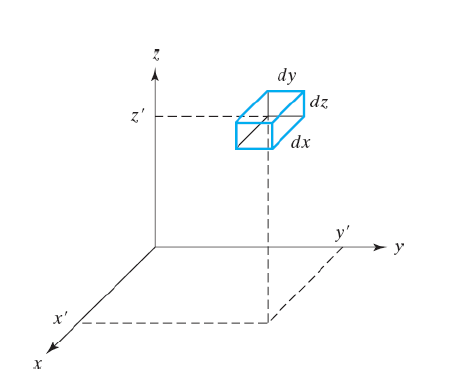
\includegraphics[width=0.5\textwidth]{Figures/3.1.png}  % 图片路径
		\caption{\text{位于}$x^{\prime}, y^{\prime},z^{\prime}$的一个无穷小箱形区域}
		\label{fig:3.1}
	\end{figure}
	虽然(\ref{eq:3.53})看起来很困难,但我们将在第 6 章中解决它。

	对于单粒子一维系统,玻恩假设[式(\ref{exp:1.15 probability of a particle})]表明:$\left|\Psi\left(x^{\prime},t\right)^2\mathrm{d}x\right|$是在$t$时刻在$x^{\prime}$到$x^{\prime}+\mathrm{d}x$区域内找到粒子的概率,其中$x^{\prime}$是$x$的一个特定值。我们对这一假设作如下扩展:\textit{对于三维单粒子系统,表达式}
	\begin{equation}
		\boxed{
			\left|\Psi\left(x^{\prime}, y^{\prime}, z^{\prime},t\right)\right|^2 \mathrm{d}x\mathrm{d}y\mathrm{d}z
		}
		\label{exp:3.54}
	\end{equation}
	\textit{是在$x^{\prime}$到$x^{\prime}+\mathrm{d}x$、$y^{\prime}$到$y^{\prime}+\mathrm{d}y$、$z^{\prime}$到$z^{\prime}+\mathrm{d}z$这一无限小空间内找到粒子的概率。}由于找到粒子的总概率为 1,因此归一化条件为
	\begin{equation}
		\int_{-\infty}^{\infty}\int_{-\infty}^{\infty}\int_{-\infty}^{\infty}\left|\Psi\left(x^{\prime}, y^{\prime}, z^{\prime},t\right)\right|^2 \mathrm{d}x\mathrm{d}y\mathrm{d}z = 1
		\label{eq:3.55}
	\end{equation}

	\textit{对于$n$粒子的三维系统,我们假设}
	\begin{equation}
		\boxed{
			\left|\Psi\left(x_1^{\prime}, y_1^{\prime}, z_1^{\prime},x_2^{\prime}, y_2^{\prime}, z_2^{\prime},\cdots,x_n^{\prime}, y_n^{\prime}, z_n^{\prime},t\right)\right|^2 \mathrm{d}x_1\mathrm{d}y_1\mathrm{d}z_1\mathrm{d}x_2\mathrm{d}y_2\mathrm{d}z_2\cdots\mathrm{d}x_n\mathrm{d}y_n\mathrm{d}z_n
		}
		\label{eq:3.56}
	\end{equation}
	\textit{是在$\left(x_1^{\prime},y_1^{\prime},z_1^{\prime}\right)$处带边$\mathrm{d}x_1,\mathrm{d}y_1,\mathrm{d}z_1$的无限小矩形盒状区域内发现粒子1,在$\left(x_2^{\prime},y_2^{\prime},z_2^{\prime}\right)$处带边$\mathrm{d}x_2,\mathrm{d}y_2,\mathrm{d}z_2$的无限小矩形盒状区域内发现粒子2,$\cdots$,在$\left(x_n^{\prime},y_n^{\prime},z_n^{\prime}\right)$处带边$\mathrm{d}x_n,\mathrm{d}y_n,\mathrm{d}z_n$的无限小矩形盒状区域内发现粒子$n$的概率。}由于找到粒子的总概率为 1,因此归一化条件为
	\begin{equation}
		\int_{-\infty}^{\infty}\int_{-\infty}^{\infty}\int_{-\infty}^{\infty}\cdots\int_{-\infty}^{\infty}\int_{-\infty}^{\infty}\int_{-\infty}^{\infty}\left|\Psi\right|^2 \mathrm{d}x_1\mathrm{d}y_1\mathrm{d}z_1\cdots\mathrm{d}x_n\mathrm{d}y_n\mathrm{d}z_n = 1
		\label{eq:3.57}
	\end{equation}
	\textit{在量子力学中,对一个系统的全空间进行积分的习惯做法是$\int\mathbf{d}\tau$。简写式}(\ref{eq:3.55})\textit{和}(\ref{eq:3.57}),\textit{有}
	\begin{equation}
		\boxed{
			\int\left|\Psi\right|^2\mathrm{d}\tau = 1
		}
		\label{eq:3.58}
	\end{equation}
	\textit{虽然}(\ref{eq:3.58})\textit{看起来像是一个不定积分,但我们可以理解为一个定积分。}根据上下文可以理解积分变量及其范围。

	对于定态系统,$\left|\Psi\right|^2 = \left|\psi\right|^2$,及
	\begin{equation}
		\boxed{
			\int\left|\psi\right|^2\mathrm{d}\tau = 1
		}
		\label{eq:3.59}
	\end{equation}
	
\section{三维盒子中的粒子}
\label{sec:3.5 The Particle in a Three-Dimensional Box}
	目前,我们只讨论单粒子问题。在本节中,我们将考虑第 2.2 节中解决的问题的三维情况,即粒子在盒子中的情况。\\
	\begin{figure}[h!]
		\centering
		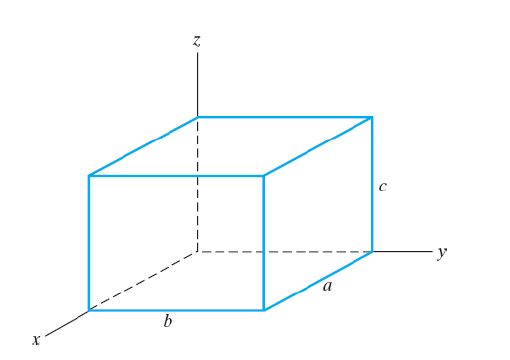
\includegraphics[width=0.5\textwidth]{Figures/3.2.png}  % 图片路径
		\caption{\text{在这个箱形区域内,}$V=0$\text{。}}
		\label{fig:3.2}
	\end{figure}

	三维盒子有多种可能的形状。我们选择的坐标系使盒子的一个角位于原点,盒子位于空间的第一卦限(图 3.2)。在盒子内,势能为零;而在盒子外,势能为无穷大:
	\begin{equation}
		V\left(x,y,z\right) = 0, \quad \text{其中}
		\begin{cases}
			0 < x < a\\
			0 < y < b\\
			0 < z < c
		\end{cases}
		\label{eq:3.60}
	\end{equation}
	\begin{equation*}
		V = \infty, \quad elsewhere
	\end{equation*}

	由于粒子具有无限能量的概率为零,因此在盒子外波函数一定为零。在盒内,势能算符为零,薛定谔方程(\ref{eq:3.47})为
	\begin{equation}
		-\frac{\hbar^2}{2m}\left(\frac{\partial^2\psi}{\partial x^2} + \frac{\partial^2\psi}{\partial y^2} + \frac{\partial^2\psi}{\partial z^2}\right) = E\psi
		\label{eq:3.61}
	\end{equation}
	为了求解 (\ref{eq:3.61}),我们假设解可以写成三个分别只与$x$、$y$和$z$有关的单独函数的乘积:
	\begin{equation}
		\psi\left(x,y,z\right) = f\left(x\right)g\left(y\right)h\left(z\right)
		\label{eq:3.62}
	\end{equation}
	我们可能会认为,这一假设抛弃了不满足 (\ref{eq:3.62}) 形式的解。然而,可以证明的是:如果我们能找到满足边界条件的 (\ref{eq:3.62}) 形式的解,那么就不存在满足边界条件的薛定谔方程的其他解了(证明见 G. F. D. Duff 和 D. Naylor, Differential Equations of Applied Mathematics, Wiley, 1966, 第 257-258 页)。我们用来求解 (\ref{eq:3.62}) 的方法称为\textbf{变量分离}(separation of variables)。

	由(\ref{eq:3.62}),我们有
	\begin{equation}
		\frac{\partial^2\psi}{\partial x^2} = f^{\prime\prime}\left(x\right)g\left(y\right)h\left(z\right), \quad \frac{\partial^2\psi}{\partial y^2} = f\left(x\right)g^{\prime\prime}\left(y\right)h\left(z\right)
		\label{eq:3.63}
	\end{equation}
	将(\ref{eq:3.63})和(\ref{eq:3.62})带入式(\ref{eq:3.61}),有
	\begin{equation}
		-\left(\hbar^2/2m\right)f^{\prime\prime}gh-\left(\hbar^2/2m\right)fg^{\prime\prime}h-\left(\hbar^2/2m\right)fgh^{\prime\prime}-Efgh = 0
		\label{eq:3.64}
	\end{equation}
	将上式左右两边同除以$fgh$,有
	\begin{equation}
		- \frac{\hbar^2f^{\prime\prime}}{2mf}- \frac{\hbar^2g^{\prime\prime}}{2mg}- \frac{\hbar^2h^{\prime\prime}}{2mh} -E = 0
		\label{eq:3.65}
	\end{equation}
	\begin{equation}
		-\frac{\hbar^2f^{\prime\prime}\left(x\right)}{2mf\left(x\right)} = \frac{\hbar^2g^{\prime\prime}\left(y\right)}{2mg\left(y\right)}+\frac{\hbar^2h^{\prime\prime}\left(z\right)}{2mh\left(z\right)}+E
		\label{eq:3.66}
	\end{equation}

	令$E_x$与上式的左边相等,有
	\begin{equation}
		E_x \equiv -\hbar^2f^{\prime\prime}\left(x\right)/2mf\left(x\right)
		\label{eq:3.67}
	\end{equation}
	定义(\ref{eq:3.67})表明$E_x$与$y$和$z$无关,方程(\ref{eq:3.66})表明$E_x$等于$\hbar^2g^{\prime\prime}\left(y\right)/2mg\left(y\right)+\hbar^2h^{\prime\prime}\left(z\right)/2mh\left(z\right)+E$;因此,$E_x$也与$x$无关。综上所述,$E_x$一定是与$x$、$y$和$z$都无关的常数。

	与(\ref{eq:3.67})类似,我们定义$E_y$与$E_z$:
	\begin{equation}
		E_y \equiv -\hbar^2g^{\prime\prime}\left(y\right)/2mf\left(y\right), \quad E_z \equiv -\hbar^2h^{\prime\prime}\left(z\right)/2mh\left(z\right)
		\label{eq:3.68}
	\end{equation}
	由于 $x$、$y$、$z$ 在 (\ref{eq:3.65}) 中对称出现,因此与证明 $E_x$ 是常数的推理相同,$E_y$ 和 $E_z$ 也是常数。将定义(\ref{eq:3.67})和(\ref{eq:3.68})代入(\ref{eq:3.65})可得
	\begin{equation}
		E_x+E_y+E_z=E
		\label{eq:3.69}
	\end{equation}

	方程(\ref{eq:3.67})和(\ref{eq:3.68})为
	\begin{equation}
		\frac{\mathrm{d}^2f\left(x\right)}{\mathrm{d}x^2}+\frac{2m}{\hbar^2}E_xf\left(x\right) = 0
		\label{eq:3.70}
	\end{equation}
	\begin{equation}
		\frac{\mathrm{d}^2g\left(y\right)}{\mathrm{d}y^2}+\frac{2m}{\hbar^2}E_yg\left(y\right) = 0, \quad \frac{\mathrm{d}^2h\left(z\right)}{\mathrm{d}z^2}+\frac{2m}{\hbar^2}E_zh\left(z\right) = 0
		\label{eq:3.71}
	\end{equation}
	我们已将三变量的偏微分方程转换为三个常微分方程。(\ref{eq:3.70}) 的边界条件是什么?由于波函数在盒外消失,因此连续性要求波函数$\psi$在盒壁处消失。特别是,在 $yOz$ 平面上的盒壁上必须为零,此处$x=0$;此外,在箱体的平行壁上必须为零,其中$x=a$。因此,$f\left(0\right) = f\left(a\right) = 0$。

	现在将公式 (\ref{eq:3.70}) 与一维盒子中粒子的薛定谔方程 [公式 (\ref{eq:2.10 schrödinger equation for particle between 0 and l}) ] 进行比较。方程的形式相同,(\ref{eq:3.70}) 中的 $E_x$ 与 (\ref{eq:2.10 schrödinger equation for particle between 0 and l}) 中的 $E$ 相对应。边界条件是否相同?是的,只是自变量消失的第二点是 $x=a$,而不是 $x=l$。因此,我们可以利用第 2.2 节中的工作来写出解[见式 (\ref{eq:2.23 stationary state wave function for the particle in a box}) 和 (\ref{eq:2.20 energy of one-dimensional box}) ]。
	\begin{equation*}
		f\left(x\right) = \left(\frac{2}{a}\right)^{1/2}\sin\left(\frac{n_x\pi x}{a}\right)
	\end{equation*}
	\begin{equation*}
		E_x = \frac{n_x^2h^2}{8ma^2}, \quad n_x = 1,2,3\cdots
	\end{equation*}
	将同样的推理应用于 $y$ 和 $z$ 方程,可以得出
	\begin{equation*}
		g\left(y\right) = \left(\frac{2}{b}\right)^{1/2}\sin\left(\frac{n_y\pi y}{b}\right), \quad h\left(z\right) = \left(\frac{2}{c}\right)^{1/2}\sin\left(\frac{n_z\pi z}{c}\right)
	\end{equation*}
	\begin{equation*}
		E_y = \frac{n_y^2h^2}{8mb^2}, \quad n_x = 1,2,3\cdots, \quad E_z = \frac{n_z^2h^2}{8mc^2}, \quad n_z = 1,2,3\cdots
	\end{equation*}

	由(\ref{eq:3.69}),能量为
	\begin{equation}
		E = \frac{h^2}{8m}\left(\frac{n_x^2}{a^2}+\frac{n_y^2}{b^2}+\frac{n_z^2}{c^2}\right)
		\label{eq:3.72}
	\end{equation}
	与一维盒子中的粒子一样,基态能量大于经典力学的最低能量值0。

	由式(\ref{eq:3.62}),箱中粒子的波函数为
	\begin{equation}
		\psi\left(x,y,z\right) = \left(\frac{8}{abc}\right)^{1/2}\sin\left(\frac{n_x\pi x}{a}\right)\sin\left(\frac{n_y\pi y}{b}\right)\sin\left(\frac{n_z\pi z}{c}\right)
		\label{eq:3.73}
	\end{equation}

	波函数有三个量子数$n_x$、$n_y$和$n_z$,我们将其归因于问题的三维性质。三个量子数彼此独立变化。

	在一维单粒子问题中,节点满足$\psi\left(x\right)=0$,解这个方程,我们就得到了$\psi = 0$的$x$值。而在三维单粒子问题中,节点满足$\psi\left(x,y,z\right) = 0$,从方程中解出$z$,我们有$z=f\left(x,y\right)$,每个这样的解都是三维空间中一个\textbf{节面}(nodal surface)的方程。例如,对于$n_x=1$、$n_y=1$、$n_z=2$的定态,令波函数($\ref{eq:3.73}$)为0,解得节面为$z=c/2$,这是一个平面的方程,该平面平行于盒子的顶面和底面,并且位于这两个面的中间。同样地,对于状态$n_x=2$、$n_y=1$、$n_z=1$,节面为$x=a/2$的平面。

	由于波函数中的$x$、$y$和$z$因子可以独立归一化,将波函数归一化,有
	\begin{equation*}
		\int_{-\infty}^{\infty}\int_{-\infty}^{\infty}\int_{-\infty}^{\infty}\left|\psi\right|^2\mathrm{d}x\mathrm{d}y\mathrm{d}z = \int_{0}^{a}\left|f\left(x\right)\right|^2\mathrm{d}x\int_{0}^{b}\left|g\left(y\right)\right|^2\mathrm{d}y\int_{0}^{c}\left|h\left(z\right)\right|^2\mathrm{d}z=1
	\end{equation*}
	其中我们用到了
	\begin{equation}
		\boxed{
			\int\int\int F\left(x\right)G\left(y\right)H\left(z\right)\mathrm{d}x\mathrm{d}y\mathrm{d}z = \int F\left(x\right)\mathrm{d}x\int G\left(y\right)\mathrm{d}y\int H\left(z\right)\mathrm{d}z
		}
		\label{eq:3.74}
	\end{equation}

	式(\ref{eq:3.73})中$\psi\left(x,y,z\right)$的量纲是什么?对于单粒子三维系统,$\left|\psi\right|^2\mathrm{d}x\mathrm{d}y\mathrm{d}z$是概率,概率是没有量纲的。由于$\mathrm{d}x\mathrm{d}y\mathrm{d}z$的量纲为长度$^3$,则为了使$\left|\psi\right|^2\mathrm{d}x\mathrm{d}y\mathrm{d}z$无量纲,$\psi\left(x,y,z\right)$一定具有长度$^{-3/2}$的量纲。

	假设$a=b=c$,则我们得到了一个立方体。能级为
	\begin{equation}
		E = \left(h^2/8ma^2\right)\left(n_x^2+n_y^2+n_z^2\right)
		\label{eq:3.75}
	\end{equation}
	让我们用表格列出被限制在立方体势箱中粒子的一些允许能量:
	\begin{equation*}
		\begin{array}{c|c|c|c|c|c|c|c|c|c|c|c}
			n_xn_yn_z & 111 & 211 & 121 & 112 & 122 & 212 & 221 & 113 & 131 & 311 & 222 \\
			\hline E\left(8ma^2/h^2\right) & 3 & 6 & 6 & 6 & 9 & 9 & 9 & 11 & 11 & 11 & 12
		\end{array}
	\end{equation*}
	\begin{figure}[h!]
		\centering
		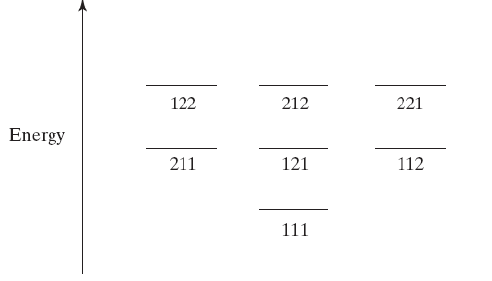
\includegraphics[width=0.5\textwidth]{Figures/3.3.png}  % 图片路径
		\caption{\text{立方体盒子中粒子最低几个状态的能量。}}
		\label{fig:3.3}
	\end{figure}
	
	请注意:量子数不同的状态可能具有相同的能量(图\ref{fig:3.3})。例如,状态$\psi_{211}$、$\psi_{121}$和$\psi_{112}$(下标表示量子数)都具有相同的能量。然而,公式 (\ref{eq:3.73}) 表明这三组量子数给出了三个不同的独立波函数,因此确实代表了系统的不同状态。当两个或两个以上的独立波函数对应于具有相同能量本征值的状态时,该本征值是\textbf{简并}(degenerate)的。一个能级的\textbf{简并度}(degree of degeneracy or simply degeneracy)就是具有该能量的状态的数量。因此,立方体中粒子的次低能级是三重简并的。当我们令盒子的边长相等时,就得到了简并的现象。简并度通常与系统的对称性有关。注意波函数态$\psi_{211}$、$\psi_{121}$和$\psi_{112}$可以通过旋转立方体盒相互转化。通常,一维问题中的束缚态能级是非简并的。

	在对理想气体的分子分配函数进行统计力学评估时,将每个气体分子的平移能级视为三维矩形盒子(盒子是容纳气体的容器)中的粒子能级;见Levine,《物理化学》,第 21.6 和 21.7 节。

	在金属的自由电子理论中,非过渡金属的价电子被视为一个盒子中的非相互作用粒子,盒子的两侧是金属的表面。这种近似方法虽然粗糙,但对金属的某些性质给出了相当不错的结果。
	
\section{简并}
\label{sec:3.6 Degeneracy}
	对于一个$n$重简并的能级,有$n$个独立的波函数$\psi_1$,$\psi_2$,$\psi_3$,$\cdots$,$\psi_n$每个波函数均有本征值$w$:
	\begin{equation}
		\hat{H}\psi_1 = w\psi_1, \quad\hat{H}\psi_2 = w\psi_2, \cdots,\quad \hat{H}\psi_n = w\psi_n
		\label{eq:3.76}
	\end{equation}
	我们想要证明以下重要理论:\textit{具有能量本征值 $w$ 的简并波函数的每一个线性组合}
	\begin{equation}
		\phi \equiv c_1\psi_1 + c_2\psi_2 + c_3\psi_3 + \cdots + c_n\psi_n
		\label{eq:3.77}
	\end{equation}
	\textit{也是能量本征函数,且具有相同的能量本征值 $w$。} [式(\ref{eq:3.77})是函数$\psi_1$,$\psi_2$,$\psi_3$,$\cdots$,$\psi_n$\textbf{线性组合}的定义。其中$c$是常数,有些可能为零。]为了证明这个理论,我们必须指明$\hat{H}\phi = w\phi$,或者
	\begin{equation}
		\hat{H}\left(c_1\psi_1 + c_2\psi_2 +  \cdots + c_n\psi_n\right) = w\left(c_1\psi_1 + c_2\psi_2 + \cdots + c_n\psi_n\right)
		\label{eq:3.78}
	\end{equation}	
	由于$\hat{H}$是线性算符,我们可以对式(\ref{eq:3.78})的左边应用式(\ref{eq:3.9})$n-1$次,有
	\begin{equation*}
		\hat{H}\left(c_1\psi_1 + c_2\psi_2 +  \cdots + c_n\psi_n\right) = \hat{H}\left(c_1\psi_1\right) + \hat{H}\left(c_2\psi_2\right) + \cdots + \hat{H}\left(c_n\psi_n\right)
	\end{equation*}
	再使用式(\ref{eq:3.10}),则(\ref{eq:3.79})变为
	\begin{equation*}
		\begin{aligned}
			\hat{H}\left(c_1\psi_1 + c_2\psi_2 +  \cdots + c_n\psi_n\right) &= c_1\hat{H}\psi_1 + c_2\hat{H}\psi_2 +  \cdots + c_n\hat{H}\psi_n \\
			&= c_1w\psi_1 + c_2w\psi_2 +  \cdots + c_nw\psi_n \\
			\hat{H}\left(c_1\psi_1 + c_2\psi_2 +  \cdots + c_n\psi_n\right) &= w\left(c_1\psi_1 + c_2\psi_2 +  \cdots + c_n\psi_n\right)
		\end{aligned}
	\end{equation*}
	这就证明了我们的理论。

	例如,在立方势箱中粒子的定态波函数$\psi_{211}$、$\psi_{121}$和$\psi_{112}$是简并的,则它们的线性组合$c_1\psi_{211} + c_2\psi_{121} + c_3\psi_{112}$立方势箱中粒子哈密顿算符的本征函数,且具有相同的能量本征值$6h^2/8ma^2$,与$\psi_{211}$、$\psi_{121}$和$\psi_{112}$相同。

	 注意:若$\psi_1$和$\psi_2$对应于不同的能量本征值($\hat{H}\psi_1 = E_1\psi_1$,$\hat{H}\psi_2 = E_2\psi_2$,且$E_1 \neq E_2$),则它们的线性组合$c_1\psi_1+c_2\psi_2$不是能量算符$\hat{H}$的本征函数。

	由于与简并能级相对应的波函数的任何线性组合都是具有相同本征值的 $\hat{H}$ 的本征函数,因此我们可以为任何简并能级构造出无数个不同的波函数。事实上,我们只对线性无关的本征函数感兴趣。若$f_1,f_2,\cdots,f_n$当且仅当所有常数$c_1,c_2,\cdots,c_n$都为零时,满足关系式$c_1f_1+c_2f_2+\cdots+c_nf_n=0$,则称$f_1,f_2,\cdots,f_n$是\textbf{线性无关}的。这就意味着\textit{在一组线性独立函数中,没有一个函数可以用其余函数的线性组合来表示。}例如,函数$f_1=3x$,$f_2=5x^2-x$,$f_3=x^2$不是线性无关的,因为$f_2=5f_3-\frac{1}{3}f_1$。而函数$g_1=1$,$g_2=x$,$g_3=x^2$是线性无关的,因为没有一个函数可以用其余函数的线性组合来表示。

	 一个能级的\textbf{简并度}等于与该能值相对应的线性独立波函数的数目。一维自由粒子波函数 (\ref{eq:2.30}) 是两个线性独立函数的线性组合,这两个函数分别是具有相同能量本征值 $E$ 的本征函数。因此每个这样的能级(除了$E=0$)都是二重简并的(简并度为2)。

\section{平均值}
\label{sec:3.7 Average Values}
	第3.3节指出:若态函数$\Psi$不是算符$\hat{B}$的本征函数,则对$B$的观测将得到一组可能值($\hat{B}$的本征值的其中一个)。我们现在考虑具有状态$\Psi$的系统的性质$B$的平均值。
	为了在实验中找到 $B$ 的平均值,我们需要许多相同的、不相互影响的系统$\Psi$,每个系统都处于相同的状态,然后测量每个系统中的 $B$。$B$的\textbf{平均值}(average value),记作$\langle B \rangle$,定义为所有测量值$b_1,b_2,\cdots,b_N$的算术平均:
	\begin{equation}
		\langle B \rangle = \frac{1}{N}\sum_{j=1}^{N}B_j
		\label{eq:3.79}
	\end{equation}
	其中系统的数目$N$是很大的一个数。

	我们可以对 $B$ 的所有可能值求和,而不是对 $B$ 的观测值求和,将每个可能值乘以观测到的次数,得到等价表达式
	\begin{equation}
		\langle B \rangle = \frac{1}{N}\sum_{b}n_bb
		\label{eq:3.80}
	\end{equation}
	其中 $n_b$ 是观测到的值 $b$ 的次数。举一个例子就会很清楚。假设一个班级的五名学生进行了五道题的测试,取得的分数为:0,20,20,60,60,80,80,80,100。则用式(\ref{eq:3.79})计算平均分,我们有
	\begin{equation*}
		\frac{1}{N}\sum_{j=2}^{N}B_j = \frac{0+20+20+60+60+80+80+80+100}{9} = \frac{500}{9} = 56
	\end{equation*}
	用式(\ref{eq:3.80})计算平均分,对所有可能的分数:0,20,40,60,80,100求和,我们有
	\begin{equation*}
		\frac{1}{N}\sum_{b}n_bb = \frac{1\left(0\right)+2\left(20\right)+0\left(40\right)+2\left(60\right)+3\left(80\right)+1\left(100\right)}{9} = \frac{500}{9} = 56
	\end{equation*}

	方程(\ref{eq:3.80})可以写作
	\begin{equation*}
		\langle B \rangle = \sum_{b}\left(\frac{n_b}{N}\right)b
	\end{equation*}
	由于$N$很大,$n_b/N$是观测到值$b$的概率$P_b$,因此
	\begin{equation}
		\langle B \rangle = \sum_{b}P_bb
		\label{eq:3.81}
	\end{equation}

	现在考虑态函数为$\Psi\left(x,t\right)$的一维单粒子系统中$x$坐标的平均值。$x$ 坐标的取值范围是连续的,在$x$到$x+\mathrm{d}x$的无限小区间内找到粒子的概率为$\left|\Psi\right|^2\mathrm{d}x$。对无限小区间的求和等同于对整个 $x$ 范围的积分,因此 (\ref{eq:3.81}) 变为
	\begin{equation}
		\langle x \rangle = \int_{-\infty}^{\infty}x\left|\Psi\left(x,t\right)\right|^2\mathrm{d}x
		\label{eq:3.82}
	\end{equation}
	对于单粒子三维系统,在位于$\left(x,y,z\right)$,具有边长$\mathrm{d}x,\mathrm{d}y,\mathrm{d}z$的体积微元内找到粒子的概率为
	\begin{equation}
		\left|\Psi\left(x,y,z,t\right)\right|^2\mathrm{d}x\mathrm{d}y\mathrm{d}z
		\label{eq:3.83}
	\end{equation}
	如果我们想知道在$x$到$x+\mathrm{d}x$的范围内找到粒子的概率,我们必须用$y$和$z$的所有可能取值对式(\ref{eq:3.83})进行积分,由于当$x$在$x+\mathrm{d}x$范围内时,粒子的$y$和$z$坐标可以任意取值。因此,对于三维的例子,式(\ref{eq:3.82})变为
	\begin{equation}
		\langle x \rangle = \int_{-\infty}^{\infty}\left[\int_{-\infty}^{\infty}\int_{-\infty}^{\infty}\left|\Psi\left(x,y,z,t\right)\right|^2\mathrm{d}y\mathrm{d}z\right]x\mathrm{d}x
		\label{eq:3.84}
	\end{equation}
	\begin{equation*}
		\langle x \rangle = \int_{-\infty}^{\infty}\int_{-\infty}^{\infty}\int_{-\infty}^{\infty}x\left|\Psi\left(x,y,z,t\right)\right|^2\mathrm{d}x\mathrm{d}y\mathrm{d}z
	\end{equation*}

	现在,我们来看看某种物理特性 $B\left(x,y,z\right)$ 的平均值,它是粒子坐标的函数。一个例子就是势能函数$V\left(x,y,z\right)$。根据式 (\ref{eq:3.84}) 的相同推理,可以得出
	\begin{equation}
		\langle B\left(x,y,z\right) \rangle = \int_{-\infty}^{\infty}\int_{-\infty}^{\infty}\int_{-\infty}^{\infty}\left|\Psi\left(x,y,z,t\right)\right|^2B\left(x,y,z\right)\mathrm{d}x\mathrm{d}y\mathrm{d}z
		\label{eq:3.85}
	\end{equation}
	\begin{equation}
		\langle B\left(x,y,z\right) \rangle = \int_{-\infty}^{\infty}\int_{-\infty}^{\infty}\int_{-\infty}^{\infty}\Psi^{\ast}B\Psi\mathrm{d}x\mathrm{d}y\mathrm{d}z
		\label{eq:3.86}
	\end{equation}
	式(\ref{eq:3.86}) 的形式似乎有点异想天开,因为它与 (\ref{eq:3.85}) 没有什么不同。但稍后我们将看到它的重要意义。

	一般来说,对于单粒子三维系统,属性 $B$ 既取决于坐标,也取决于动量:
	\begin{equation*}
		B = B\left(x,y,z,p_x,p_y,p_z\right)
	\end{equation*}
	我们如何找到$B$的平均值?我们\textit{假设}处于$\Psi$状态的系统的$\langle B \rangle$为
	\begin{equation*}
		\langle B \rangle = \int_{-\infty}^{\infty}\int_{-\infty}^{\infty}\int_{-\infty}^{\infty}\Psi^{\ast}B\left(x,y,z,\frac{\hbar^2}{\mathrm{i}}\frac{\partial}{\partial x},\frac{\hbar^2}{\mathrm{i}}\frac{\partial}{\partial y},\frac{\hbar^2}{\mathrm{i}}\frac{\partial}{\partial z}\right)\Psi\mathrm{d}x\mathrm{d}y\mathrm{d}z
	\end{equation*}
	\begin{equation}
		\langle B \rangle = \int_{-\infty}^{\infty}\int_{-\infty}^{\infty}\int_{-\infty}^{\infty}\Psi^{\ast}\hat{B}\Psi\mathrm{d}x\mathrm{d}y\mathrm{d}z
		\label{eq:3.87}
	\end{equation}
	其中$\hat{B}$是性质$B$的量子力学算符。[稍后,我们将利用 (\ref{eq:3.87}) 来证明含时薛定谔方程在从量子力学到经典力学的转变过程中还原为牛顿第二定律,从而为这一假设提供一些理由;见问题 7.59。],对于$n$粒子体系,我们假设
	\begin{equation}
		\boxed{
			\langle B \rangle = \int \Psi^{\ast}\hat{B}\Psi\mathrm{d}\tau
		}
		\label{eq:3.88}
	\end{equation}
	其中$\int\mathrm{d}\tau$表示对全空间的$3n$坐标的积分。由于我们将$\Psi^{\ast}\Psi$视为概率密度,式(\ref{eq:3.88})中的态函数必须先归一化。重要的是,要将算符放在在$\Psi^{\ast}$和$\Psi$中间。表达式$\hat{B}\Psi^{\ast}\Psi$、$\Psi^{\ast}\Psi\hat{B}$和$\Psi^{\ast}\hat{B}\Psi$的含义是不同的,除非$B$只是坐标的函数。在$\int\Psi^{\ast}\hat{B}\Psi\mathrm{d}\tau$中,第一个操作是将算符$\hat{B}$应用于态函数$\Psi$,然后将结果与$\Psi^{\ast}$相乘并对全空间进行积分,就得到了$\langle B \rangle$。

	对于定态,我们有[式\ref{eq:1.20}]
	\begin{equation*}
		\Psi^{\ast}\hat{B}\Psi = \mathrm{e}^{\mathrm{i}Et/\hbar}\psi^{\ast}\hat{B}\mathrm{e}^{-\mathrm{i}Et/\hbar}\psi = \mathrm{e}^{0}\psi^{\ast}\hat{B}\psi = \psi^{\ast}\hat{B}\psi
	\end{equation*}
	由于$\hat{B}$不包含对时间的导数,也不会影响 $\Psi$ 中的时间因子,因此,对于定态,有
	\begin{equation}
		\langle B \rangle = \int \psi^{\ast}\hat{B}\psi\mathrm{d}\tau
		\label{eq:3.89}
	\end{equation}
	因此,在定态系统中,若$\hat{B}$与时间无关,则$\langle B \rangle$也是与时间无关的。

	考虑一个特殊的例子,若$\Psi$是$\hat{B}$的本征函数。当$\hat{B}\Psi = k\Psi$时,式(\ref{eq:3.88})变为
	\begin{equation*}
		\langle B \rangle = \int \Psi^{\ast}\hat{B}\Psi\mathrm{d}\tau = \int \Psi^{\ast}k\Psi\mathrm{d}\tau = k \int \Psi^{\ast}\Psi\mathrm{d}\tau = k
	\end{equation*}
	其中$\Psi$已归一化。由于当$\hat{B}\Psi = k\Psi$时,$k$ 是我们在测量时能找到的唯一可能的 $B$ 值,因此这个结果是合理的(第 3.3 节)。

	由式(\ref{eq:3.88})很容易证明以下关于平均值的性质(见问题 3.49):
	\begin{equation}
		\boxed{
			\langle A + B \rangle = \langle A \rangle + \langle B \rangle
		}
		\quad
		\boxed{
			\langle cB \rangle = c\langle B \rangle
		}
		\label{eq:3.90}
	\end{equation}
	其中$A$和$B$是系统的物理量,$c$是常数。但是,平均值的乘积不一定等于乘积的平均值:$\langle AB \rangle \neq \langle A \rangle\langle B \rangle$。

	通常使用\textbf{期望值}(expectation value)一词来代替平均值。期望值并不一定是我们观察到的可能值之一。
	\begin{examplebox}
		\textbf{例题:}对于处于基态的三维单粒子系统,求$\langle x \rangle$和$\langle p_x \rangle$的值。\\
		
		将基态波函数$\psi=f\left(x\right)g\left(y\right)h\left(z\right)$[式(\ref{eq:3.62})]代入式(\ref{eq:3.89}),有
		\begin{equation*}
			\langle x \rangle = \int \psi^{\ast}\hat{x}\psi \mathrm{d}\tau = \int_{0}^{c}\int_{0}^{b}\int_{0}^{a}f^{\ast}g^{\ast}h^{\ast} x fgh\mathrm{d}x\mathrm{d}y\mathrm{d}z
		\end{equation*}
		而在势箱外有$\psi = 0$。由于$g\left(y\right)$和$h\left(z\right)$已归一化,使用式(\ref{eq:3.74}),我们有
		\begin{equation*}
			\langle x \rangle = \int_{0}^{a} x\left|f\left(x\right)\right|^{2}\mathrm{d}x \int_{0}^{b}\left|g\left(y\right)\right|^{2}\mathrm{d}y \int_{0}^{c}\left|h\left(z\right)\right|^{2}\mathrm{d}z = \int_{0}^{a} x\left|f\left(x\right)\right|^{2}\mathrm{d}x
		\end{equation*}
		由于系统处于基态,有$n_x=1$,则$f\left(x\right) = \left(2/a\right)^{1/2}\sin\left(\pi x/a\right)$,因此
		\begin{equation}
			\langle x \rangle = \frac{2}{a}\int_{0}^{a} x\sin^{2}\left(\frac{\pi x}{a}\right)\mathrm{d}x = \frac{a}{2}
			\label{eq:3.91}
		\end{equation}
		其中我们用到了附录中的(A.3)。根据图\ref{fig:2.4},这个结果是合理的。

		同样地,
		\begin{equation*}
			\langle p_x \rangle = \int \psi^{\ast}\hat{p}_x\psi \mathrm{d}\tau = \int_{0}^{c}\int_{0}^{b}\int_{0}^{a}f^{\ast}g^{\ast}h^{\ast} \frac{\hbar}{\mathrm{i}}\frac{\partial}{\partial x}\left[f\left(x\right)g\left(y\right)h\left(z\right)\right]\mathrm{d}x\mathrm{d}y\mathrm{d}z
		\end{equation*}
		\begin{equation*}
			\langle p_x \rangle = \frac{\hbar}{\mathrm{i}}\int_{0}^{a}f^{\ast}\left(x\right)f^{\prime}\left(x\right)\mathrm{d}x \int_{0}^{b}\left|g\left(y\right)\right|^{2}\mathrm{d}y \int_{0}^{c}\left|h\left(z\right)\right|^{2}\mathrm{d}z
		\end{equation*}
		\begin{equation}
			\langle p_x \rangle = \frac{\hbar}{\mathrm{i}}\int_{0}^{a}f\left(x\right)f^{\prime}\left(x\right)\mathrm{d}x = \frac{\hbar}{2\mathrm{i}}\left. f^2\left(x\right) \right|_{0}^{a} = 0
			\label{eq:3.92}
		\end{equation}

		其中,我们用到了定解条件$f\left(0\right)=f\left(a\right)=0$。由于粒子向$+x$和$-x$方向的移动是等概率的,因此这个结果是合理的。\\
		
		\textbf{练习:}求处于基态的三维单粒子系统的$\langle p_x^2 \rangle$的值。\\
		(\textit{答案:}$h^2/4l^2$。)
	\end{examplebox}

\section{波函数的约束条件}
\label{sec:3.8 Requirements for an Acceptable Wave Function}
	在求解箱中粒子的问题时,我们要求$\psi$是连续的。我们现在讨论波函数需要满足的其他约束条件。

	由于$\left|\psi\right|^2\mathrm{d}\tau$是概率,我们希望可以通过选择一个合适的\textbf{归一化常数}(normalization constant)与波函数相乘,使得波函数可以归一化。若$\psi$未归一化而$N\psi$已归一化,则根据归一化条件,有
	\begin{equation}
		1 = \int \left|N\psi\right|^2\mathrm{d}\tau = N^2\int \left|\psi\right|^2\mathrm{d}\tau
		\label{eq:3.93}
	\end{equation}
	\begin{equation*}
		N = \left(\int \left|\psi\right|^2\mathrm{d}\tau\right)^{-1/2}
	\end{equation*}

	只有当$\psi$处处为零时,定积分$\int \left|\psi\right|^2\mathrm{d}\tau$才为零。然而,$\psi$不可能处处为零(这意味着没有粒子存在)。因此,这个积分一定不会为零。若$\int \left|\psi\right|^2\mathrm{d}\tau$为无穷大,则$\left|N\right|$为零,$\psi$就无法归一化。当且仅当$\int \left|\psi\right|^2\mathrm{d}\tau$具有有限而非无限值时,我们才能对$\psi$进行归一化。如果对全空间的积分$\int \left|\psi\right|^2\mathrm{d}\tau$为有限值,我们说$\psi$是\textbf{平方可积的}(quadratically integrable)。因此,我们一般要求$\psi$是平方可积的。一个最重要的例外不处于束缚态的粒子。因此,粒子在势阱中(第 2.4 节)的非束缚态和自由粒子的波函数都不是平方可积的。
	\begin{figure}[ht]
		\centering
		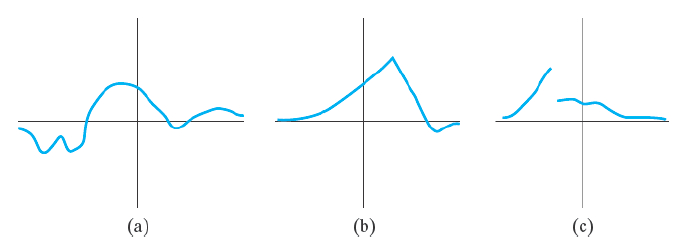
\includegraphics[width=0.6\textwidth]{Figures/3.4.png}  % 图片路径
		\caption{
			\centering
			\parbox{0.4\linewidth}{
   		 		\noindent
    			函数(a)是连续函数,其一阶导数也连续;函数(b)是连续函数,但其一阶导数不连续;函数(c)不是连续函数。
			}
		}
		\label{fig:3.4}
	\end{figure}

	由于$\psi^{\ast}\psi$是概率密度,因此波函数一定是单值的。如果我们的理论对在某一点发现粒子的概率给出了两个不同的值,那就太尴尬了。如果我们要求$\psi$是单值的,那么显然$\psi^{\ast}\psi$也是单值的。$\psi$可能会有多个值[例如,$\psi\left(q\right) = -1,1,\mathrm{i}$],但$\psi^{\ast}\psi$只能有一个值。然而,我们仍要求$\psi$是单值的。

	除了要求$\psi$是连续,我们也通常要求其偏导数$\partial\psi/\partial x$,$\partial\psi/\partial y$等也是连续的(见图\ref{fig:3.4}a)。不过,回过头来看第 2.2 节,我们会发现:对于箱中粒子$\partial\psi/\partial x$在箱壁上不连续,以及$\partial\psi/\partial x$在箱外为零,但是由方程(\ref{eq:2.23 stationary state wave function for the particle in a box})可知,$\partial\psi/\partial x$在箱壁上又不为零。$\psi^{\prime}$的不连续性是由在箱壁处势能突然变为无穷大造成的。对于具有有限高度的势垒来说,$\psi^{\prime}$在箱壁处是连续的。

	与平方可积的要求一致,有时也会说波函数必须在任何地方都是有限的,包括无穷大。然而,这通常是比平方可积性更强的要求。事实上,氢原子的一些相对论波函数在原点处是无限的,但却是平方可积的。偶尔,我们也会遇到在原点处无限大的非相对论波函数 [L. D.D. 兰道和 E. M. 利夫希茨,《量子力学》,第三版(1977 年),第 35 节]。因此,基本要求是平方可积性,而不是有限性。

	我们要求任何代表物理量的算符的本征函数都满足上述要求。符合这些要求的函数被称为\textbf{品优函数}(well-behaved function)。

\section*{总结}

\section*{习题}
	
	% ===== CHAPTER 4 =====
\chapter{谐振子}
\label{chap:4}
    我们将在第 13.2 节中看到,气相分子的能量可以近似为平动、转动、振动和电子能量之和。电子能量的计算将在第 13 章至第 17 章中讨论。平动能是分子作为一个整体在容纳物质的容器空间中的运动动能。平动能级可视为三维空间中粒子的能级(第 3.5 节)。二原子(双原子)分子的转动能级可以用刚性转子的转动能级来近似表示,第 6.4 节将对此进行讨论。双原子分子的最低几个振动能级可以用谐振子的能级来近似表示(第 4.3 节),多原子分子的振动能可以用线性谐振子振动能之和来近似表示(第 15.12 节)。本章第 4.2 节将求解谐振子的薛定谔方程。作为初步介绍,第 4.1 节讨论了求解微分方程的幂级数解法,该方法用于求解谐振子的薛定谔方程。第 4.3 节讨论分子振动。第 4.4 节介绍了求一维薛定谔方程特征值和特征函数的数值方法。
\section{微分方程的幂级数解}
\label{sec:4.1 Power-Series Solutions of Differential Equations}
    到目前为止,我们只考虑了势能$V\left(x\right)$是常数的情况。这使得薛定谔方程成为一个具有常数系数的二阶线性齐次微分方程,我们知道如何求解这个方程。对于 $V$ 随 $x$ 变化的情况,一种有用的方法是尝试薛定谔方程的幂级数解法。

    为了说明这种方法,考虑微分方程
    \begin{equation}
        y^{\prime\prime}\left(x\right) + c^2 y\left(x\right) = 0
        \label{eq:4.1}
    \end{equation}
    其中$c^2>0$。当然,这个微分方程有常系数,但我们可以用幂级数法求解。让我们先用特征方程$s^2+c^2=0$来求解这个方程。特征方程的根是$s=\pm \mathrm{i}c$。回忆第 2.2 节中的工作[公式 (\ref{eq:2.10 schrödinger equation for particle between 0 and l}) 和 (\ref{eq:4.1}) 是相同的],当特征方程的根是纯虚数时,我们会得到三角函数形式的通解:
    \begin{equation}
        y\left(x\right) = A \cos\: cx + B \sin\: cx
        \label{eq:4.2}
    \end{equation}
    其中 $A$ 和 $B$ 是积分常量。式(\ref{eq:4.2})的另一种形式是
    \begin{equation}
        y = D \sin\left(cx+e\right)
        \label{eq:4.3}
    \end{equation}
    其中 $D$ 和 $e$ 是任意常数。利用两角之和的正弦公式,我们可以证明 (\ref{eq:4.3}) 等价于 (\ref{eq:4.2})。

    现在让我们用幂级数法来求解 (\ref{eq:4.1})。我们假设方程的解可以在$x=0$处展开成Taylor级数的形式(见问题:4.1),也就是说,我们假设
    \begin{equation}
        y\left(x\right) = \sum_{n=0}^{\infty}a_nx^n = a_0 + a_1 x + a_2 x^2 + a_3 x^3 + \cdots
        \label{eq:4.4}
    \end{equation}
    其中 $a$ 为常数系数,有待确定,以使式 (\ref{eq:4.1}) 成立。对式(\ref{eq:4.4})求导,有
    \begin{equation}
        y^{\prime}\left(x\right) = a_1 + 2a_2 x + 3a_3 x^2 + \cdots = \sum_{n=1}^{\infty}na_nx^{n-1}
        \label{eq:4.5}
    \end{equation}
    其中,我们假设该数列可以逐项求导(对于无穷级数来说,这并不总是正确的)。对于$y^{\prime\prime}$,我们有
    \begin{equation}
        y^{\prime\prime}\left(x\right) = 2a_2 + 3\left(2\right)a_3 x + \cdots = \sum_{n=2}^{\infty}n(n-1)a_nx^{n-2}
        \label{eq:4.6}
    \end{equation}
    将 (\ref{eq:4.6}) 和 (\ref{eq:4.4}) 代入 (\ref{eq:4.1}),得到
    \begin{equation}
        \sum_{n=2}^{\infty}n(n-1)a_nx^{n-2} + c^2\sum_{n=0}^{\infty}a_nx^n = 0
        \label{eq:4.7}
    \end{equation}
    我们想把 (\ref{eq:4.7}) 中的两个和合并起来。只要满足一定条件,我们就可以将两个无穷级数逐项相加,得到它们的和:
    \begin{equation}
        \sum_{j=0}^{\infty}b_jx^j + \sum_{j=0}^{\infty}c_jx^j = \sum_{j=0}^{\infty}(b_j+c_j)x^j
        \label{eq:4.8}
    \end{equation}
    要将 (\ref{eq:4.8}) 应用于 (\ref{eq:4.7}) 中的两个和,我们希望每个和的极限相同,$x$ 的幂相同。因此,我们改变了 (\ref{eq:4.7}) 中第一个和的下标,定义$k \equiv n-2$。极限$n = 2$到无穷大与$k = 0$到无穷大相对应,将$n=k+2$代入第一个和,有
    \begin{equation}
        \sum_{n=2}^{\infty}n\left(n-1\right)a_nx^{n-2} = \sum_{k=0}^{\infty}\left(k+2\right)\left(k+1\right)a_{k+2}x^k = \sum_{n=0}^{\infty}\left(n+2\right)\left(n+1\right)a_{n+2}x^n
        \label{eq:4.9}
    \end{equation}
    (\ref{eq:4.9}) 中的最后一个等式是有效的,因为求和指数是一个\textbf{虚拟变量}(dummy variable);我们用什么字母来表示这个变量没有区别。例如,求和$\sum_{i=1}^{3}c_ix^i$和$\sum_{m=1}^{3}c_mx^m$是相等的,因为它们只有求和指数不同。如果我们将这个求和展开就会更好理解:
    \begin{equation*}
        \sum_{i=1}^{3}c_ix_6 = c_1x^1 + c_2x^2 + c_3x^3, \quad \sum_{m=1}^{3}c_mx^m = c_1x^1 + c_2x^2 + c_3x^3
    \end{equation*}
    在 (\ref{eq:4.9}) 的最后一个等式中,我们只是将表示求和指数的符号从 $k$ 改为 $n$。定积分中的积分变量也是一个虚拟变量,因为定积分的值不受变量字母的影响:
    \begin{equation}
        \int_{a}^{b}f\left(x\right)dx = \int_{a}^{b}f\left(t\right)dt
        \label{eq:4.10}
    \end{equation}
    将式(\ref{eq:4.9}) 代入 (\ref{eq:4.7}),我们得到
    \begin{equation}
        \sum_{n=0}^{\infty}\left[\left(n+2\right)\left(n+1\right)a_{n+2}+c^2a_n\right]x^n = 0
        \label{eq:4.11}
    \end{equation}
    如果 (\ref{eq:4.11}) 对所有 $x$ 值都成立,那么 $x$ 的每个幂的系数都必须为零。为了说明这一点,请看方程
    \begin{equation}
        \sum_{j=0}^{\infty}b_jx^j = 0
        \label{eq:4.12}
    \end{equation}
    在式(\ref{eq:4.12}),令$x=0$,我们有$b_0=0$。将式(\ref{eq:4.12})左右两侧对$x$求导,则$b_1=0$。求$n$阶导数,令$x=0$,我们得到$b_n=0$。因此,从式(\ref{eq:4.11})中,我们有:
    \begin{equation}
        \left(n+2\right)\left(n+1\right)a_{n+2} + c^2 a_n = 0
        \label{eq:4.13}
    \end{equation}
    \begin{equation}
        a_{n+2} = -\frac{c^2}{\left(n+1\right)\left(n+2\right)}a_n
        \label{eq:4.14}
    \end{equation}
    方程(\ref{eq:4.14}) 是一个\textbf{递推关系式}(recursion relation),如果我们知道$a_0$的值,就能用式(\ref{eq:4.14})计算出$a_2$、$a_4$、$a_6$等的值。如果我们知道$a_1$的值,就能用式(\ref{eq:4.14})计算出$a_3$、$a_5$、$a_7$等的值。由于对$a_0$和$a_1$的选择没有限制,它们是任意常数,我们分别用$A$和$Bc$来表示:
    \begin{equation}
        a_0 = A, \quad a_1 = Bc
        \label{eq:4.15}
    \end{equation}
    则利用式(\ref{eq:4.14}),我们可以计算系数:
    \begin{equation*}
        a_0 = A, \quad a_2 = -\frac{c^2}{1 \cdot 2}A, \quad a_4 = \frac{c^4}{1 \cdot 2\cdot 3}A, \quad a_6 = -\frac{c^6}{6!}A, \quad \ldots
    \end{equation*}
    \begin{equation}
        a_{2k} = (-1)^k \frac{c^{2k}}{(2k)!}A, \quad k = 0, 1, 2, \ldots
        \label{eq:4.16}
    \end{equation}
    \begin{equation*}
        a_1 = Bc, \quad a_3 = -\frac{c^3}{2 \cdot 3}Bc, \quad a_5 = \frac{c^5}{2 \cdot 3 \cdot 4 \cdot 5}Bc, \quad a_7 = -\frac{c^7}{7!}Bc, \quad \ldots
    \end{equation*}
    \begin{equation}
        a_{2k+1} = (-1)^k \frac{c^{2k+1}}{(2k+1)!}B, \quad k = 0, 1, 2, \ldots
        \label{eq:4.17}
    \end{equation}
    根据式(\ref{eq:4.4})、 (\ref{eq:4.16}) 和 (\ref{eq:4.17}) 我们有
    \begin{equation}
        y = \sum_{n=0}^{\infty}a_nx^n = \sum_{n=0,2,4, \cdots}^{\infty}a_nx^n + \sum_{n=1,3,5, \cdots}^{\infty}a_nx^n
        \label{eq:4.18}
    \end{equation}
    \begin{equation}
        y = A\sum_{k=0}^{\infty}(-1)^k\frac{c^{2k}x^{2k}}{(2k)!} + B\sum_{k=0}^{\infty}(-1)^k\frac{c^{2k+1}x^{2k+1}}{(2k+1)!}
        \label{eq:4.19}
    \end{equation}
    (\ref{eq:4.19}) 中的两个级数是 $\cos\: cx$ 和 $\sin\: cx$ 的Taylor级数(问题:4.2)。因此,与式(\ref{eq:4.2}) 相同,我们有$y = \cos\: cx + \sin\: cx$。

\section{一维谐振子}
\label{sec:4.2 The One-Dimensional Harmonic Oscillator}
    在本节中,我们将通过求解一维谐振子的薛定谔方程来增加我们的量子力学知识。该系统是分子振动的重要模型。
    
\subsection*{经典力学的处理}
    在研究谐振子的波动力学之前,我们先回顾一下经典的处理方法。我们有一个质量为 $m$ 的单粒子,它被一个与粒子离原点的位移成正比的力吸引向原点:
    \begin{equation}
        F_x = -kx
        \label{eq:4.20}
    \end{equation}
    比例常数$k$称为\textbf{力常数}(force constant)。$F_x$是作用在粒子上的力在$x$方向上的分量。这也是这个一维问题中的总力。附着在弹簧上的质点遵守公式 (\ref{eq:4.20}),前提是弹簧没有从平衡位置大幅拉伸。

    由牛顿第二定律$F = ma$,我们有
    \begin{equation}
        - kx = m\frac{\mathrm{d}^2x}{\mathrm{d}t^2}
        \label{eq:4.21}
    \end{equation}
    其中$t$是时间。若令$c^2 = k/m$,则式(\ref{eq:4.21})与式(\ref{eq:4.1})相同。因此,其解为[将$c = \left(k/m\right)^{1/2}$代入式(\ref{eq:4.3})],有
    \begin{equation}
        x = A \sin\left(2\pi \nu t +b\right)
        \label{eq:4.22}
    \end{equation}
    其中$A$是\textbf{振幅}(the amplitude of vibration),$b$是积分常数,\textbf{振动频率}(vibration frequency)$\nu$是
    \begin{equation}
        \boxed{
            \nu = \frac{1}{2\pi}\left(\frac{k}{m}\right)^{1/2}
        }
        \label{eq:4.23}
    \end{equation}
    由于正弦函数的最大最小值分别为1和-1,相应地,满足式(\ref{eq:4.22}) 的$x$值在$A$和$-A$之间振荡。正弦函数的最小正周期为$2\pi$,则完成一次完整振荡所需的时间(称为\textbf{周期}(period))为正弦函数参数增加$2\pi$的时间。在$t+1/\nu$时刻,正弦函数的参数为$2\pi \nu \left(t+1/\nu\right) + b = 2\pi \nu t + 2\pi + b$,比$t$时刻的参数多了$2\pi$。因此,周期为$1/\nu$。周期的倒数就是单位时间内的振动次数(振动频率),因此频率为$\nu$。

    现在我们来考虑能量。在三维系统中,势能$V$与力的分量的关系为
    \begin{equation}
        \boxed{
            F_x = -\frac{\mathrm{d}V}{\mathrm{d}x}, \quad F_y = -\frac{\mathrm{d}V}{\mathrm{d}y}, \quad F_z = -\frac{\mathrm{d}V}{\mathrm{d}z}
        }
        \label{eq:4.24}
    \end{equation}
    方程(\ref{eq:4.24}) 是势能的定义。由于这是一个一维系统,我们有[式(\ref{eq:1.12 Potential energy in classical mechanics})]
    \begin{equation}
        F_x = -\frac{\mathrm{d}V}{\mathrm{d}x} = -kx
        \label{eq:4.25}
    \end{equation}
    对(\ref{eq:4.25})两边积分,我们得到$V = \int kx \mathrm{d}x = \frac{1}{2}kx^2 + C$,其中$C$是积分常数。势能总是有一个任意的附加常数。我们令$C = 0$,则
    \begin{equation}
        \boxed{
            V = \frac{1}{2}kx^2
        }
        \label{eq:4.26}
    \end{equation}
    将式(\ref{eq:4.23})带入,有
    \begin{equation}
        V = 2\pi^2 \nu^2 m x^2
        \label{eq:4.27}
    \end{equation}
    势能$V$的图象是一个抛物线。动能$T$可以由式(\ref{eq:4.22})对时间$t$求导得到:
    \begin{equation}
        T = \frac{1}{2}m\left(\frac{\mathrm{d}x}{\mathrm{d}t}\right)^2
        \label{eq:4.28}
    \end{equation}
    将$T$和$V$相加,我们得到了总能量:
    \begin{equation}
        E = T + V = \frac{1}{2}kA^2 = 2\pi\nu^2mA^2
        \label{eq:4.29}
    \end{equation}
    其中我们用到了$\sin^2\theta + \cos^2\theta = 1$。

    根据式(\ref{eq:4.22}),经典力学中的谐振子在$x=A$和$x=-A$之间振荡运动。这两点是运动的转折点。在这两点,粒子的速度为零,而在$x=0$处速度达到最大值,同时势能为零而动能最大。经典的谐振子在$x=A$和$x=-A$附近的运动会比在$x=0$附近花费更多的时间(速度最慢)。问题 4.18 计算了在不同位置找到经典谐振子的概率密度。(有趣的是,这个概率密度在转折点处变得无限大)
    
\subsection*{量子力学的处理}
    由式(\ref{eq:3.27})和(\ref{eq:4.27}),谐振子的哈密顿算符为
    \begin{equation}
        \hat{H} = -\frac{\hbar^2}{2m}\frac{\mathrm{d}^2}{\mathrm{d}x^2} + 2\pi^2 \nu^2 m x^2 = -\frac{\hbar^2}{2m}\left(\frac{\mathrm{d}^2}{\mathrm{d}x^2} - \alpha^2x^2\right)
        \label{eq:4.30}
    \end{equation}
    其中,为了书写方便,我们定义了$\alpha$为
    \begin{equation}
        \alpha \equiv 2\pi\nu m/\hbar
        \label{eq:4.31}
    \end{equation}
    乘上$2m/\hbar^2$后,薛定谔方程$\hat{H}\psi = E\psi$变为
    \begin{equation}
        \frac{\mathrm{d}^2\psi}{\mathrm{d}x^2} + \left(2mE\hbar^{-2}-\alpha^2x^2\right)\psi = 0
        \label{eq:4.32}
    \end{equation}
    现在我们可以尝试求得 (\ref{eq:4.32}) 的幂级数解。如果我们现在考虑具有式(\ref{eq:4.4})形式的$\psi$幂级数,我们会发现它推出了一个三项递推关系,这比式 (\ref{eq:4.14}) 这样的两项递推关系更难处理。因此,我们修改 (\ref{eq:4.32}) 的形式,以便在尝试幂级数解时能得到两项的递推关系。能实现这一目的的替代方法(见问题 4.22)是$f\left(x\right) \equiv \mathrm{e}^{\alpha x^2/2}\psi\left(x\right)$。因此,
    \begin{equation}
        \psi = \mathrm{e}^{-\alpha x^2/2}f\left(x\right)
        \label{eq:4.33}
    \end{equation}
    这个方程只是定义了一个新函数$f\left(x\right)$,取代 $\psi\left(x\right)$ 作为未知函数来求解。(我们可以在微分方程中进行任何替换)对式(\ref{eq:4.33})两边求导两次,得到
    \begin{equation}
        \psi^{\prime\prime} = \mathrm{e}^{-\alpha x^2/2}\left(f0-2\alpha xf^{\prime} - \alpha f + \alpha^2x^2f\right)
        \label{eq:4.34}
    \end{equation}
    将(\ref{eq:4.34})和(\ref{eq:4.33})代入(\ref{eq:4.32}),我们得到
    \begin{equation}
        f^{\prime\prime}\left(x\right) - 2\alpha x f^{\prime}\left(x\right) + \left(2mE\hbar^{-2} - \alpha\right)f\left(x\right) = 0
        \label{eq:4.35}
    \end{equation}
    现在我们可以尝试幂级数解。假设
    \begin{equation}
        f\left(x\right) = \sum_{n=0}^{\infty}c_nx^N
        \label{eq:4.36}
    \end{equation}
    假设可以对式(\ref{eq:4.36})逐项求导,我们有
    \begin{equation}
        f^{\prime}\left(x\right) = \sum_{n=1}^{\infty}nc_nx^{n-1} = \sum_{n=0}^{\infty}nc_nx^{n-1}
        \label{eq:4.37}
    \end{equation}
    [式(\ref{eq:4.37})中第二个加和的第一项为零]。同样地,
    \begin{equation*}
        f^{\prime\prime}\left(x\right) = \sum_{n=2}^{\infty}n(n-1)c_nx^{n-2} = \sum_{j=0}^{\infty}(j+2)(j+1)c_{j+2}x^{j} = \sum_{n=0}^{\infty}(n+2)(n+1)c_{n+2}x^{n}
    \end{equation*}
    其中,我们令$j = n - 2$,然后将求和指数从 $j$ 改为 $n$ [见公式 (\ref{eq:4.9})]。代入 (\ref{eq:4.35}),我们得到
    \begin{equation*}
        \sum_{n=0}^{\infty}\left(n+2\right)\left(n+1\right)c_{n+2}x^n - 2\alpha \sum_{n=0}^{\infty}n c_n x^n + \left(2mE\hbar^{-2} - \alpha\right)\sum_{n=0}^{\infty}c_nx^n = 0
    \end{equation*}
    \begin{equation}
        \sum_{n=0}^{\infty}\left[(n+2)(n+1)c_{n+2} - 2\alpha n c_n + \left(2mE\hbar^{-2} - \alpha\right)c_n\right]x^n = 0
        \label{eq:4.38}
    \end{equation}
    令$x^n$的系数为零[与式(\ref{eq:4.11})一致],我们得到
    \begin{equation}
        c_{n+2} = \frac{\alpha + 2\alpha n - 2mE\hbar^2}{(n+1)(n+2)}c_n
        \label{eq:4.39}
    \end{equation}
    这正是我们想要的两项递推关系。式(\ref{eq:4.39})与式(\ref{eq:4.14})类似,知道了$c_n$的值,就可以计算出$c_{n+2}$的值。因此,我们有了两个任意常数$c_0$和$c_1$。如果我们令$c_1=0$,那么我们将得到一个只包含 $x$ 的偶数次幂乘以指数因子的幂级数作为解:
    \begin{equation}
        \psi = \mathrm{e}^{-\alpha x^2/2}f\left(x\right) = \mathrm{e}^{-\alpha x^2/2}\sum_{n=0,2,4,\cdots}^{\infty}c_{n}x^{n} = \mathrm{e}^{-\alpha x^2/2}\sum_{l=0}^{\infty}c_{2l}x^{2l}
        \label{eq:4.40}
    \end{equation}
    如果我们令$c_0=0$,那么我们将得到另一个独立的解:
    \begin{equation}
        \psi = \mathrm{e}^{-\alpha x^2/2}f\left(x\right) = \mathrm{e}^{-\alpha x^2/2}\sum_{n=1,3,5,\cdots}^{\infty}c_{n}x^{n} = \mathrm{e}^{-\alpha x^2/2}\sum_{l=0}^{\infty}c_{2l+1}x^{2l+1}
        \label{eq:4.41}
    \end{equation}
    薛定谔方程的通解为上述两个独立解的线性组合:
    \begin{equation}
        \psi = A\mathrm{e}^{-\alpha x^2/2}\sum_{l=0}^{\infty}c_{2l+1}x^{2l+1} + B\mathrm{e}^{-\alpha x^2/2}\sum_{l=0}^{\infty}c_{2l}x^{2l}
        \label{eq:4.42}
    \end{equation}
    其中 $A$ 和 $B$ 是任意常数。

    现在我们必须看看波函数的边界条件是否会对解法产生任何限制。为了了解这两个无穷级数在$x$充分大时的表现,我们要考察每个级数中连续系数的比值。在第二个级数中,$x^{2l+2}$与$x^{2l}$的比值为[在(\ref{eq:4.39})中令$n=2l$]:
    \begin{equation*}
        \frac{c_{2l+2}}{c_{2l}} = \frac{\alpha + 4\alpha l - 2mE\hbar^2}{(2l+1)(2l+2)}
    \end{equation*}
    假设对于较大的 $x$ 值,级数中的后项是主要项,那么我们就来看看对于较大的 $l$ 值,这一比值是多少:
    \begin{equation}
        \frac{c_{2l+2}}{c_{2l}} \sim \frac{4\alpha l}{4l^2} = \frac{\alpha}{l} \quad \text{当}l\text{很大时}
        \label{eq:4.43}
    \end{equation}
    在(\ref{eq:4.39})中令$n=2l+1$,我们发现,当 $l$ 较大时,第一个序列中连续系数的比值也是 $\alpha/l$。 现在考虑函数 $\mathrm{e}^{\alpha x^2}$ 的幂级数展开。(问题 4.3)
    \begin{equation}
        \mathrm{e}^{z} = \sum_{n=0}^{\infty}\frac{z^n}{n!} = 1 + z + \frac{z^2}{2!} + \cdots
        \label{eq:4.44}
    \end{equation}
    我们有
    \begin{equation*}
        \mathrm{e}^{\alpha x^2} = 1 + \alpha x^2 + \cdots + \frac{\alpha ^l x^{2l}}{l!} + \frac{\alpha ^{l+1} x^{2l+2}}{(l+1)!} + \cdots
    \end{equation*}
    在该级数中,$x^{2l+2}$和$x^{2l}$的系数比为
    \begin{equation*}
        \frac{\alpha^{l+1}}{\left(l+1\right)!} \div \frac{\alpha^l}{l!} = \frac{\alpha}{l+1} \sim \frac{\alpha}{l} \quad \text{当}l\text{很大时}
    \end{equation*}
    因此,解 (\ref{eq:4.42}) 中每个无穷级数的连续系数比与$l$很大时的级数$\mathrm{e}^{\alpha x^2}$相同。因此,我们可以得出结论:当$x$很大时,每个级数的行为都与 $\mathrm{e}^{\alpha x^2}$ 相同。[这不是一个严格的证明。H. A. Buchdahl, Am. J. Phys. J. Phys., 42, 47 (1974); see also M. Bowenand J. Coster, Am. J. Phys., 48, 307 (1980)]

    如果每个级数的行为都与 $\mathrm{e}^{\alpha x^2}$ 相同,那么当 $x$ 很大时,$\psi$ 的行为也将与 $\mathrm{e}^{\alpha x^2}$ 相同。当$x$趋于无穷时,波函数的值将趋于无穷大,就不满足波函数平方可积的要求。如果我们可以将级数在某一项打断,使得级数的后续项为零,那么因子$\mathrm{e}^{\alpha x^2}$就能保证在$x$趋于无穷时,$\psi$的值趋于零。(使用L' Hopital法则,显然当$x \to \infty$时,有$x^p\mathrm{e}^{-\alpha x^2} \to 0$,$p$为任意有限次幂)若想让级数在某一有限项后被打断,则当$n$为某个值时必须有递推公式(\ref{eq:4.39})中$c_n$的系数为零,记$n=v$。这就使得$c_{v+2}$、$c_{v+4}$$\cdots$等全为零。而式(\ref{eq:4.42})中的一个级数将具有有限项。在递推关系 (\ref{eq:4.39}) 中,有一个量的值尚未确定,但可以通过调整,使$c_v$消失。这个量就是能量$E$。在(\ref{eq:4.39}中)令$c_v$的系数为零,对$\alpha$使用式(\ref{eq:4.31}),我们有
    \begin{equation*}
        \alpha + 2\alpha v - 2mE\hbar^{-2} = 0
    \end{equation*}
    \begin{equation*}
        2mE\hbar^{-2} = \left(2v+1\right)2\pi\nu m/\hbar^{-1}
    \end{equation*}
    \begin{equation}
        \boxed{
            E = \left(v+\frac{1}{2}\right)h\nu, \quad v = 0, 1, 2, \ldots
        }
        \label{eq:4.45}
    \end{equation}
    \begin{figure}[ht]
        \centering
        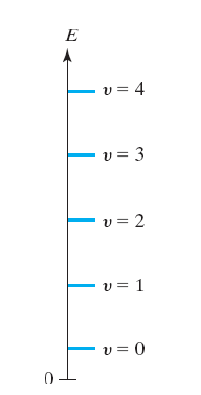
\includegraphics[width=0.2\textwidth]{Figures/4.1.png}
        \caption{\text{一维谐振子最低的五个能级图}}
        \label{fig:4.1}
    \end{figure}
    谐振子定态能级 (\ref{eq:4.45}) 间距相等(图\ref{fig:4.1})。不要混淆量子数$v$(vee)和振动频率$\nu$(nu)。

     将(\ref{eq:4.45})代入(\ref{eq:4.39}),我们得到
    \begin{equation}
        c_{n+2} = \frac{2\alpha \left(n-v\right)}{(n+1)(n+2)}c_n
        \label{eq:4.46}
    \end{equation}

    根据(\ref{eq:4.45})对能量进行量子化,我们已经使其中一个级数在有限项后被打断。为了消除 (\ref{eq:4.42}) 中的另一个无穷级数,我们必须将与之相乘的任意常数设为零。这样,根据 $v$ 是偶数还是奇数,波函数就是只包含 $x$ 的偶次或奇次幂的有限幂级数的 $\mathrm{e}^{-\alpha x^2/2}$ 倍。在该级数中,由于我们选择的能量$E$使得$c_{v+2}$、$c_{v+4}$,$\cdots$全消失,则$x$的最高次幂为$v$。因此,波函数(\ref{eq:4.42})的形式为
    \begin{equation}
        \psi_v = 
        \begin{cases}
            \mathrm{e}^{-\alpha x^2/2}\left(c_0+c_2x^2+ \cdots + c_vx^v\right), & \text{当} v \text{为偶数时} \\
            \mathrm{e}^{-\alpha x^2/2}\left(c_1x+c_3x^3+ \cdots + c_vx^v\right), & \text{当} v \text{为奇数时}
        \end{cases}
        \label{eq:4.47}
    \end{equation}
    其中任意常数$A$与$B$可被包含在$c_0$和$c_1$中,因此可以略去。$c_0$和$c_1$之后的系数可以通过递推关系式(\ref{eq:4.46})计算得到。由于量子数$v$出现在了递推关系中,对于不同的$v$值,我们可以得到一组不同的系数$c_i$。例如,$\psi_4$中的$c_2$与$\psi_2$中的$c_2$是不同的。
    \begin{figure}[ht]
        \centering
        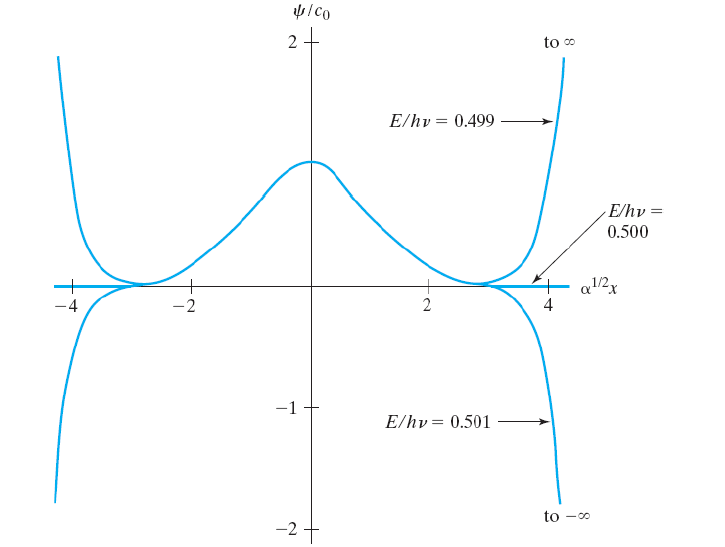
\includegraphics[width=0.75\textwidth]{Figures/4.2.png}
        \caption{
            \centering
            \parbox{0.5\linewidth}{
                \noindent
                当 $E = 0.499h\nu$、$E = 0.500h\nu$ 和 $E = 0.501h\nu$ 时,谐振子薛定谔方程的解只包含 $x$ 的偶次幂。在 $x = 0$ 附近的区域,三条曲线几乎重合。当 $|\alpha^{1/2} x| > 3$ 时,$E = 0.500h\nu$ 的曲线几乎与 $x$ 轴重合。
            }
        }
        \label{fig:4.2}
    \end{figure}

    与盒中粒子一样,波函数必须是品优波函数的要求迫使我们将能量量子化。对于不满足式(\ref{eq:4.45})的能量,$\psi$不是平方可积的。例如,图\ref{fig:4.2}显示了能量分别满足$E = 0.499h\nu$、$E = 0.500h\nu$和$E = 0.501h\nu$。当 $E = 0.500h\nu$ 时,式(\ref{eq:4.40})中的$\psi$,其中我们用到了递推关系(\ref{eq:4.39})来计算系数$c_n$(另见问题4.23)。图\ref{fig:4.2}显示了这些曲线在$\alpha^{1/2}x$附近区域的放大图。

    谐振子的基态能量不为零。这个能量$\frac{1}{2}h\nu$被称为\textbf{零点能量}(zero-point energy)。这是在绝对零度的温度下,谐振子集合中谐振子的振动能量。零点能可以由不确定性原理来理解。如果最低态的能量为零,那么它的势能和动能(均为非负值)都必须为零。动能为零则意味着动量也为零,那么$\Delta p_x = 0$。势能为零则意味着粒子始终处于原点,则$\Delta x = 0$。但我们不能同时让$\Delta p_x = 0$和$\Delta x = 0$,因此,基态能量必须大于零。零点能(ZPE)的定义为$E_{ZPE}=E_{gs} - V_{min}$,其中$E_{gs}$是基态能量,$V_{min}$是势能的最小值。
    \begin{figure}[ht]
        \centering
        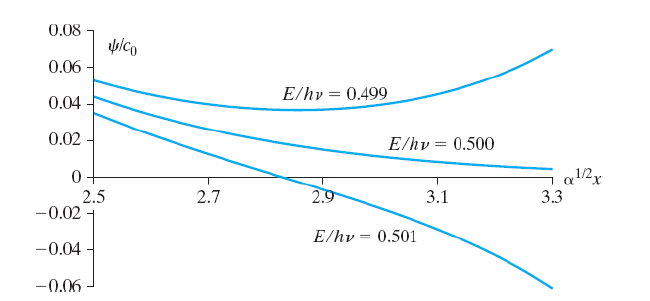
\includegraphics[width=0.75\textwidth]{Figures/4.3.png}
        \caption{
            图\ref{fig:4.2}在$\alpha^{1/2}x$附近区域的放大图。
        }
        \label{fig:4.3}
    \end{figure}

\subsection*{偶函数和奇函数}
    在详细考察波函数之前,我们先定义奇函数和偶函数。如果函数$f\left(x\right)$
    \begin{equation}
        \boxed{
            f\left(-x\right) = f\left(x\right)
        }
        \label{eq:4.48}
    \end{equation}
    则称$f\left(x\right)$为\textbf{偶函数}(even function)。因为$\left(-x\right)^2 = x^2$和$\mathrm{e}^{-b\left(x^2\right)} = \mathrm{e}^{-b\left(-x^2\right)}$,所以$x^2$和$\mathrm{e}^{bx^2}$均是偶函数。偶函数的图象关于$y$轴对称(例如,见图\ref{fig:4.4}a)。因此,对于偶函数,有
    \begin{equation}
        \boxed{
            \int_{-a}^{+a}f\left(x\right)\mathrm{d}x = 2\int_{0}^{a}f\left(x\right)\mathrm{d}x
        }
        \label{eq:4.49}
    \end{equation}
    如果$g\left(x\right)$满足
    \begin{equation}
        \boxed{
            g\left(-x\right) = -g\left(x\right)
        }
        \label{eq:4.50}
    \end{equation}
    则称$g\left(x\right)$为\textbf{奇函数}(odd function)。例如$x$、$1/x$和$x^3\mathrm{e}^{x^2}$。在式(\ref{eq:4.50})中,令$x=0$,若$g\left(0\right)$存在且为单值,则$g\left(0\right) = 0$。奇函数的图形大致如图\ref{fig:4.4} b 所示。由于 $y$ 轴一侧的正贡献会被另一侧相应的负贡献抵消,我们可以得出:对于奇函数,有
    \begin{equation}
        \boxed{
            \int_{-a}^{+a}g\left(x\right)\mathrm{d}x = 0
        }
        \label{eq:4.51}
    \end{equation}
    \begin{figure}[ht]
        \centering
        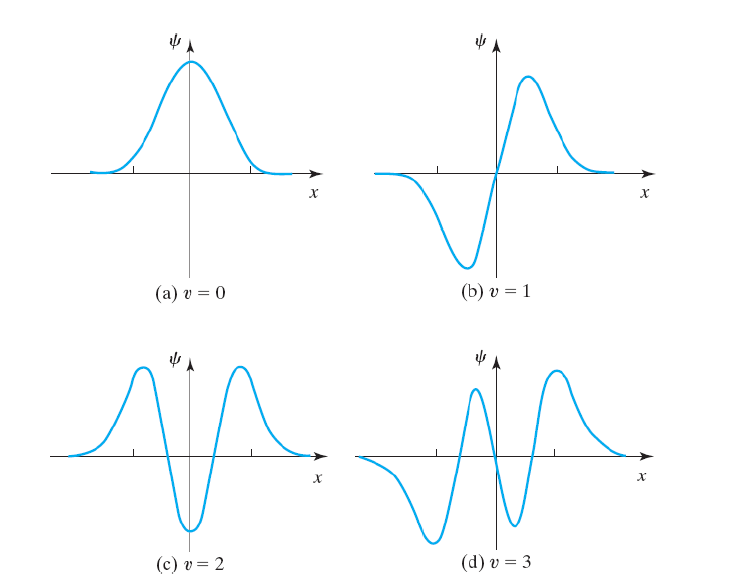
\includegraphics[width=0.75\textwidth]{Figures/4.4.png}
        \caption{
                \centering
                \parbox{0.5\linewidth}{
                \noindent
                谐振子波函数。所有图形使用相同的比例尺。$x$ 轴上标记的点为$\alpha^{1/2} x=\pm 2$。
            }
        }
        \label{fig:4.4}
    \end{figure}

    很容易证明,两个偶函数或两个奇函数的乘积是偶函数,而一个偶函数和一个奇函数的乘积是奇函数。
    
\subsection*{谐振子波函数}
    式(\ref{eq:4.47})中的指数部分$\mathrm{e}^{-\alpha x^2/2}$是偶函数。若$v$是偶数,则多项式因子只包含$x$的偶次幂,使得$\psi_v$是偶函数。若$v$是奇数,则多项式因子只包含$x$的奇次幂,使得$\psi_v$是一个奇函数和一个偶函数的乘积,为奇函数。每一个谐振子状态方程$\psi$都是一个奇函数或偶函数,取决于$v$的奇偶性。在第\ref{sec:7.5 Parity}节中,我们将看到:当势能函数$V$是偶函数时,非简并能级的波函数一定是奇函数或偶函数。

    现在,我们找到了最低三个能级波函数的显式。对于$v=0$的基态,式(\ref{eq:4.47})给出
    \begin{equation}
        \psi_0 = c_0\mathrm{e}^{-\alpha x^2/2}
        \label{eq:4.52}
    \end{equation}
    其中$\psi$的下标表示量子数$v$。通过归一化,我们可以求出$c_0$:
    \begin{equation*}
        1 = \int_{-\infty}^{\infty}\left|c_0\right|\mathrm{e}^{-\alpha x^2}\mathrm{d}x = 2\left|c_0\right|^2\int_{0}^{\infty}\mathrm{e}^{-\alpha x^2}\mathrm{d}x
    \end{equation*}
    其中,我们用到了式(\ref{eq:4.49})。使用附录中的积分(A.9),我们有$\left|c_0\right| = \left(\alpha/\pi\right)^{1/4}$。因此,如果我们选择令归一化常数的相位为零,则基态波函数为
    \begin{equation}
        \psi_0 = \left(\alpha / \pi\right)^{1/4}\mathrm{e}^{-\alpha x^2 /2}
        \label{eq:4.53}
    \end{equation}
    波函数 (\ref{eq:4.53}) 是一个高斯函数(图\ref{fig:4.4}a)。

    对于状态$v=1$,式(\ref{eq:4.47})给出
    \begin{equation}
        \psi_1 = c_1x\mathrm{e}^{-\alpha x^2 / 2}
        \label{eq:4.54}
    \end{equation}
    使用(A.10)进行归一化,我们有
    \begin{equation}
        \psi_1 = \left(4\alpha^3 / \pi\right)^{1/4}x\mathrm{e}^{-\alpha x^2 / 2}
        \label{eq:4.55}
    \end{equation}
    图\ref{fig:4.4}b显示了$\psi_1$的图象。

    对于状态$v=2$,式(\ref{eq:4.47})给出
    \begin{equation*}
        \psi_2 = \left(c_0 + c_2x^2\right)\mathrm{e}^{-\alpha x^2 / 2}
    \end{equation*}
    将$v=2$代入(\ref{eq:4.46}),我们有
    \begin{equation*}
        c_2 = \frac{2\alpha \left(-2\right)}{1\cdot2}c_0 = -2\alpha c_0
    \end{equation*}
    因此,
    \begin{equation}
        \psi_2 = c_0\left(1-2\alpha x^2\right)\mathrm{e}^{-\alpha x^2 / 2}
        \label{eq:4.56}
    \end{equation}
    使用归一化解出$c_0$,我们有(问题4.10)
    \begin{equation}
        \psi_2 = \left(4\alpha^3 / \pi\right)^{1/4}\left(2\alpha x^2 - 1\right)\mathrm{e}^{-\alpha x^2 / 2}
        \label{eq:4.57}
    \end{equation}
    注意:$\psi_2$中的$c_0$和$\psi_0$中的$c_0$是不同的。

    波函数节点的个数与量子数$v$相同。可以证明(见《Messiah》,第 109-110 页):\textit{对于一维定态束缚态问题,若$\psi$处于基态,则边界点内部的节点数为零;而对于每一个连续的激发态,节点数都会增加一个。}
    \begin{figure}[ht]
        \centering
        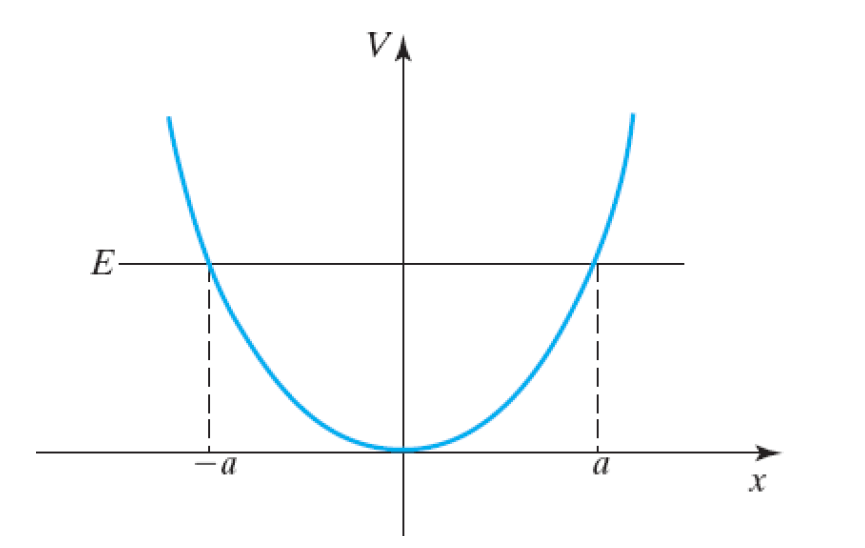
\includegraphics[width=0.65\textwidth]{Figures/4.5.png}
        \caption{
            谐振子的经典允许区域$-a \le x \le a$和禁阻区域$x > a$,$x < -a$
        }
        \label{fig:4.5}
    \end{figure}

    谐振子波函数中的多项式因子在数学中是众所周知的,被称为\textit{厄米多项式}(Hermite polynomials),是以一位法国数学家的名字命名的。(见问题 4.21)

    根据量子力学解法,在 $x$ 轴上的任何一点(节点除外)都有一定概率找到粒子。从经典角度讲,$E=T+V$,动能 $T$ 不能为负:$T \ge 0$。因此,$E-V = T \ge 0$则$V \le E$。势能 $V$ 是位置的函数,经典粒子被限制在 $V<E$ 的空间区域内。也就是说,势能不超过总能量。在图 (\ref{fig:4.5}) 中,标有 $E$ 的水平线表示谐振子的能量,抛物线表示势能 $\frac{1}{2}kx^2$。对于区域$x < -a$和$x > a$,我们有$V>E$,这些区域是\textbf{经典禁阻}(classical forbidden)的。\textbf{经典允许的区域}(classical allowed region) $-a \le x \le a$在图 (\ref{fig:4.5}) 中满足$V\le E$。

    在量子力学中,定态波函数不是算符$\hat{T}$或$\hat{V}$的本征函数,因此我们无法确定定态系统的动能或势能值。与经典力学的方程$E=T+V$和$T \ge 0$不同,在量子力学中我们有$\langle E \rangle = \langle T \rangle + \langle V \rangle$(问题6.35)和$\langle T \rangle \ge 0$(问题7.7),所以量子力学中满足$\langle V \rangle \le E$,但是我们不能写作$V \le E$,因此,粒子有一定概率在经典禁区($V>E$的区域)中被发现。

    如果说粒子可以在经典允许的区域之外被发现,我们似乎就允许它具有负动能。实际上,量子力学的观点并不存在悖论。为了验证粒子是否处于经典禁止区域,我们必须测量它的位置。这种测量会改变系统的状态(第 \ref{sec:1.3 The Uncertainty Principle} 和 \ref{sec:1.4 The Time-Dependent Schrödinger Equation} 节)。振子与测量仪器的相互作用会将足够的能量传递给振子,使其处于经典禁区。对 $x$ 的精确测量会给动量带来很大的不确定性,因此也会给动能带来很大的不确定性。\ref{sec:2.4 Particle in a Rectangular Potential Well} 节和 \ref{sec:2.5 Tunneling} 节讨论了经典禁区的穿透问题。

    一个定态谐振子满足$E = \left(v+\frac{1}{2}\right)h\nu$和$V=\frac{1}{2}kx^2 = 2\pi^2\nu^2mx^2$。因此,在经典允许的区域($V\le E$)有$2\pi^2\nu^2mx^2 \le \left(v+\frac{1}{2}\right)h\nu$,即$x^2 \le \left(v+\frac{1}{2}\right)h/2\pi^2\nu^2m = \left(2v+1\right)\alpha$,其中$\alpha \equiv 2\pi\nu m/\hbar$[式(\ref{eq:4.31})]。因此,谐振子的经典允许区域为$-\left(2v+1\right)^{1/2} \le \alpha^{1/2}x \le \left(2v+1\right)^{1/2}$。

    从图 (\ref{fig:4.4}) 中可以看出:\textit{$\psi$ 在经典允许区域中振荡,而在经典禁止区域则以指数形式下降到零。}我们之前在矩形势阱中看到过粒子的这种行为(第 \ref{sec:2.4 Particle in a Rectangular Potential Well} 节)。

    图 (\ref{fig:4.4}) 显示,当谐振子的能量逐渐升高时,$\psi$ 和 $\left|\psi\right|^2$ 的最大值往往离原点越来越远。由于离原点越远,势能$V = \frac{1}{2}kx^2$越大,平均势能$\langle V \rangle = \int_{-\infty}^{\infty}\left|\psi\right|^2V\mathrm{d}x$也会随着量子数的增加而增大。平均动能由$\langle T \rangle = -\left(\hbar^2/2m\right)\int_{-\infty}^{\infty}\psi^{\ast}\psi^{\prime\prime}\mathrm{d}x$给出。应用分部积分(问题7.7b),有$\langle T \rangle = \left(\hbar^2/2m\right)\int_{-\infty}^{\infty}\left|\mathrm{d}\psi/\mathrm{d}x\right|^2\mathrm{d}x$。量子数越大的状态中节点的数量越多,$\psi$ 的变化速度就越快,因此随着量子数的增加,$\langle T \rangle$也会增加。

    经典谐振子最有可能出现在运动转折点附近的区域,即振子运动速度最慢、$V$ 值较大的区域。相反,对于量子谐振子的基态,最有可能出现的区域是原点附近的区域。对于高振动量子数,人们会发现的外峰值大于原点附近的峰值,最可能的区域变成了经典转折点附近的区域,此时 $V$ 很大(见问题 4.18 )。这是对应原理(第 \ref{sec:2.2 Particle in a One-Dimensional Box} 节)的一个例子。

    量子谐振子的一些在线模拟可从以下网站获得:\url{www.phy.davidson.edu/StuHome/cabell_f/energy.html}(显示能级和波函数,并显示当能量从允许值改变时波函数如何发散);\url{www.falstad.com/qm1d/}(从顶部的下拉菜单中选择谐振子;双击底部的一个小圆圈以显示静止状态;显示能量、波函数、概率密度;$m$ 和 $k$ 可以改变);\url{demonrations.wolfram.com/HarmonicOscillatorEigenfunctions}(展示了$\left|\psi\right|^2$)。

\section{双原子分子的振动}
\label{sec:4.3 Vibrations of Diatomic Molecules}
    我们将在第 \ref{sec:13.1 The Born-Oppenheimer Approximation} 节中看到,在极好的近似条件下,我们可以分别处理分子中电子的运动和原子核的运动(这是由于原子核的质量要大得多)。首先想象原子核静止不动,然后求解电子能量 $U$ 的薛定谔方程($U$ 还包括核排斥能量)。对于二原子(双原子)分子,电子能量 $U$ 取决于原子核之间的距离 $R$,$U=U\left(R\right)$,而 $U$ 与 $R$ 的关系曲线则如图 13.1 所示。

    找到$U\left(R\right)$后,可以先解决核运动的薛定谔方程,使用$U\left(R\right)$作为核运动的势能函数。对于双原子分子,核薛定谔方程是一个双粒子方程。我们将在第 \ref{sec:6.3 Reduction of the Two-Particle Problem to Two One-Particle Problems} 节中看到,当双粒子系统的势能只取决于粒子之间的距离时,系统的能量是 (a) 整个系统在空间平动的动能和 (b) 粒子相对于彼此的内部运动能量之和。双粒子内部运动能量的经典表达式是粒子间相互作用的势能与假设粒子的动能之和,其中假设粒子的质量为$m_1m_2/\left(m_1+m_2\right)$($m_1$ 和 $m_2$ 分别是两个原子的质量),该粒子的坐标为一个粒子相对于另一个粒子的坐标。$m_1m_2/\left(m_1+m_2\right)$称为\textbf{约化质量}(reduced mass)$\mu$。

    二原子分子的内部运动包括\textbf{振动}和\textbf{转动},前者与两个原子核之间距离 $R$ 的变化相对应,后者与原子核连接线空间方向的变化相对应。通常可以近似地将振动和转动分开处理。转动能级见第 \ref{sec:6.4 The Two-Particle Rigid Rotor} 节。 此处我们考虑振动能级。

    双原子分子振动的薛定谔方程有一个质量为$m_1m_2/\left(m_1+m_2\right)$假设粒子的动能算符和一个由$U\left(R\right)$给出的势能项。如果我们将原点与图 13.1 中$U$曲线的最低点重合,并将该最低点的能量取为势能的零点,那么 $U(R)$ 曲线的下半部分将与具有适当力常数 $k$ 的谐振子的势能曲线几乎重合(见图 \ref{fig:4.6} 和问题 4.28)。$U(R)$ 曲线的最小值出现在\textbf{平衡核间距}(equilibrium distance)$R_e$的位置。在图 \ref{fig:4.6} 中,$x$ 是核间距与平衡核间距的偏差:$x \equiv R - R_e$。
    \begin{figure}[ht]
        \centering
        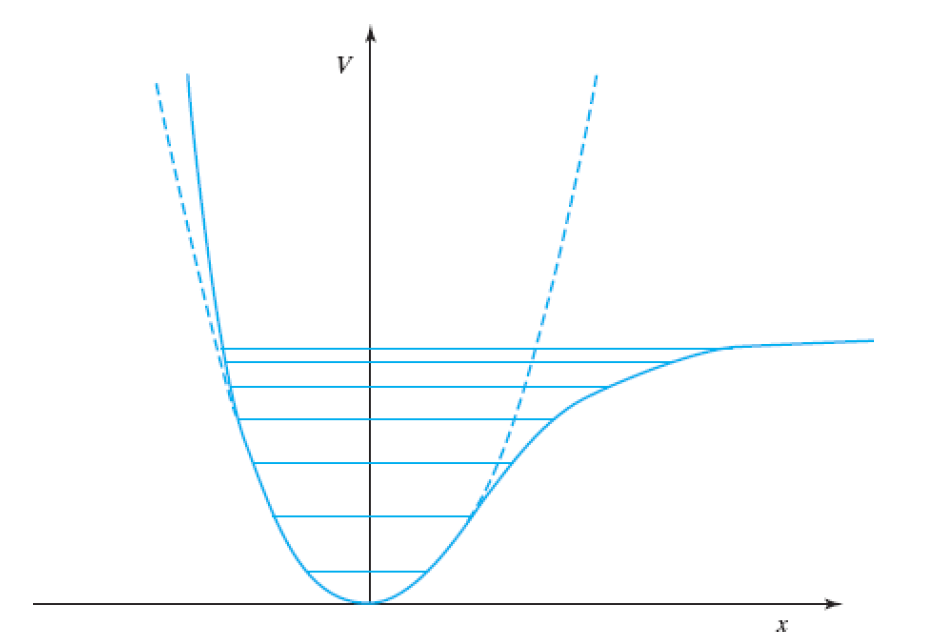
\includegraphics[width=0.7\textwidth]{Figures/4.6.png}
        \caption{
            \centering
            \parbox{0.5\linewidth}{
                \noindent
                双原子分子振动的势能(实线)和谐振子的势能(虚线)。图中还显示了二原子分子的束缚态振动能级。与谐振子相比,二原子分子只有有限数量的束缚振动能级。
            }
        }
        \label{fig:4.6}
    \end{figure}

    谐振子的力常数$k$在式(\ref{eq:4.26})中可以由$k = \mathrm{d}^2V /\mathrm{d}x^2$计算得到,在$R=R_e$处,谐振子曲线与$U(R)$曲线的下半部分几乎重合,所以分子的力常数$k = \left.\mathrm{d}^2U/\mathrm{d}R^2\right|_{R=R_e}$。(另见问题4.28)。\textit{核质量的差异对电子能量曲线 $U(R)$ 几乎没有影响,因此同一分子但由不同同位素取代的种类具有基本相同的力常数 $k$。}

    因此,我们预计二原子分子振动能级 $E_{vib}$ 的一个合理近似是谐振子振动能级;由式(\ref{eq:4.45})和式(\ref{eq:4.23}),有
    \begin{equation}
        \boxed{
            E_{vib} \approx \left(v+\frac{1}{2}\right)h\nu_e, \quad v = 0, 1, 2, \ldots
        }
        \label{eq:4.58}
    \end{equation}
    \begin{equation}
        \boxed{
            \nu_e = \frac{1}{2\pi}\left(\frac{k}{\mu}\right)^{1/2}, \quad \mu = \frac{m_1m_2}{m_1+m_2}, \quad k = \left.\frac{\mathrm{d}^2U}{\mathrm{d}R^2}\right|_{R=R_e}
        }
        \label{eq:4.59}
    \end{equation}
    其中$\nu_e$称为\textbf{简谐振动频率}(equilibrium or harmonic vibrational frequency)。这种近似方法最适用于较低的振动能级。随着$v$的增加,原子核位于远离其平衡间隔区域的时间更长。对于这些区域,势能大大偏离谐振子的势能,谐振子近似效果不佳。我们会发现:随着 $v$ 的增大,双原子分子的振动能级不是等距排列,而是越靠越近(图 \ref{fig:4.6})。最终,振动能量大到足以将双原子分子解离成互不结合的原子。与谐振子不同,双原子分子只有有限数量的束缚态振动能级。考虑到振动的非谐性,分子振动能的更精确表达式是
    \begin{equation}
        E_{vib} = \left(v+\frac{1}{2}\right)h\nu_e - \left(v+\frac{1}{2}\right)^2h\nu_e \chi_e
        \label{eq:4.60}
    \end{equation}
    其中\textit{非谐性常数}(anharmonicity constant)$\nu_e\chi_e$几乎在所有情况下都大于零。(\textit{译者注:一般认定$\chi_e$为非谐性常数?})

    使用含时薛定谔方程,我们可以发现(见第\ref{sec:9.9 Interaction of Radiation and Matter}节):当双原子分子暴露在电磁辐射下时,最有可能发生的振动跃迁是那些 $v$ 变化了 $\pm 1$ 的跃迁。此外,要吸收或发射电磁辐射,振动必须改变分子的偶极矩。因此,同核双原子分子(例如$\mathrm{H}_2$、$\mathrm{N}_2$)不能通过吸收或发射辐射实现振动能级之间的转换(这种转变可以发生在分子间碰撞中)。关系$E_{upper}-E_{lower} = h\nu$(其中$\nu$为辐射频率)、近似方程(\ref{eq:4.58})、吸收和发射辐射的\textbf{选律}(selection rule)$\Delta v = \pm 1$表明:一个振动频率为$\nu_e$的异核双原子分子将对近似为下式给出频率的辐射$\nu_{light}$有强烈吸收:
    \begin{equation}
        \nu_{light} = \left(E_2-E_1\right)/h \approx \left[\left(v_2+\frac{1}{2}\right)h\nu_e-\left(v_1+\frac{1}{2}\right)h\nu_e\right]/h = \left(v_2-v_1\right)\nu_e = \nu_E
        \label{eq:4.61}
    \end{equation}
    双原子分子$k$和$\mu$值的特性使得$\nu_{light}$通常位于光谱的红外区域。$\Delta v = 2,3,\cdots$的跃迁也会发生,但这些(称为\textit{泛频}(overtones))的吸收要比$\Delta v = 1$的跃迁弱得多。

    使用更准确的方程(\ref{eq:4.60}),有(问题4.27)
    \begin{equation}
        \nu_{light} = \nu_e - 2\nu_e\chi_e\left(v_1+1\right)
        \label{eq:4.62}
    \end{equation}
    其中$v_1$是较低能级的振动量子数,选律为$\Delta v = \pm 1$。

    热平衡系统中分子两个能级的布居数由\textbf{玻尔兹曼分布律}(Boltzmann distribution law)给出(见物理化学教材):
    \begin{equation}
        \boxed{
            \frac{N_i}{N_j} = \frac{g_i}{g_j} \mathrm{e}^{-(E_i-E_j)/kT}
        }
        \label{eq:4.63}
    \end{equation}
    其中能级$i$和$j$的能量分别为$E_i$和$E_j$,$g_i$和$g_j$是对应能级的简并度,$k$是玻尔兹曼常数,$T$是热力学温度。对于非简并能级,有$g_i=1$。

    $\nu = \left(1/2\pi\right)\left(k/\mu\right)^{1/2}$的数量级使得在室温下,对于轻分子(例如$\mathrm{H}_2$、$\mathrm{HCl}$、$\mathrm{CO}$),只有$v=0$的振动能级是被显著占据的。对于重分子(例如$\mathrm{I}_2$),在室温下有一个或多个激发态振动能级被显著占据。

    极性双原子分子的振动吸收光谱包含$v= 0 \to 1$吸收带,很弱的泛频吸收带($v = 0\to 2, 0 \to 3, \cdots$),以及若$v>0$的能级也被显著占据,也有\textit{热带}(hot bands),例如$v = 1 \to 2$、$v = 1 \to 3$等。与特定振动跃迁相对应的每个波段都由几条紧密相连的线组成。每一条这样的线都对应于与振动状态变化同时发生的不同的转动状态变化。每一条线都是振动-转动跃迁的结果。

    光谱频率的国际单位为\textbf{赫兹}(hertz,Hz),定义
    为$1 \:\mathrm{Hz} \equiv 1 \:\mathrm{s}^{-1}$。通常使用的倍数有等于 $10^6$ 赫兹的兆赫兹(MHz)和等于 $10^9$ 赫兹的千兆赫兹(GHz)。红外(IR)吸收峰通常由\textbf{波数}(wavenumber)$\tilde{\nu}$给出,定义为
    \begin{equation}
        \boxed{
            \tilde{\nu} \equiv \frac{\nu}{c} = \frac{1}{\lambda}
        }
        \label{eq:4.64}
    \end{equation}
    其中$\lambda$是真空中辐射的波长。

    在谐振子近似中,多原子分子的量子力学能级为$E_{vib} = \sum i\left(v_i+\frac{1}{2}\right)h\nu_i$,其中$\nu_i$是分子每个正则振动模式的频率,$v_i$是对应第$i$个正则振动的量子数。每个振动量子数$v_i$的取值$0,1,2,\cdots$都与其他振动量子数的取值无关。一个具有$n$个原子的线性分子具有$3n-6$个正则振动模式,而一个具有$n$个原子的非线性分子具有$3n-5$个正则振动模式。

    为了由式(\ref{eq:4.59})计算折合质量$\mu$,我们需要知道每种同位素的质量。附录表 A.3 列出了一些常见同位素的相对原子质量。

    \begin{examplebox}
        \textbf{例题:}$^{12}\mathrm{C}^{16}\mathrm{O}$分子的最强红外吸收峰位于$\tilde{\nu} = 2140 \:\mathrm{cm}^{-1}$。计算该分子的力常数 $k$。请说明所做的近似计算。\\
        
        最强的红外吸收峰对应于$v = 0 \to 1$的跃迁。我们将分子振动近似为谐振子模型。由式(\ref{eq:4.61}),分子的平衡振动频率近似为
        \begin{equation*}
            \nu_e \approx \nu_{light} = \tilde{\nu}c = \left(2140 \:\mathrm{cm}^{-1}\right)\left(2.9979 \times 10^{10} \:\mathrm{cm/s}\right)  = 6.424 \times 10^{13} \:\mathrm{s}^{-1}
        \end{equation*}
        使用式(\ref{eq:4.59}),将$k$与$\nu_e$联系起来,我们需要折合质量$\mu = m_1m_2/\left(m_1+m_2\right)$。1 mol $^{12}\mathrm{C}$的质量为12 g,包含阿伏伽德罗常数($N_A$)个分子,则一个$^{12}\mathrm{C}$原子的质量为$\left(12 \: \mathrm{g} \right)/ \left(6.02214 \times 10^{23}\right)$。折合质量和力常数分别为
        \begin{equation*}
            \mu = \frac{12 \left(15.9949\right)\: g}{27.9949} \frac{1}{6.02214 \times 10^{23}} = 1.1385 \times 10^{-23} \:\mathrm{g}
        \end{equation*}
        \begin{equation*}
            k = 4\pi^2 \nu_e^2\mu = 4\pi^2 \left(6.424 \times 10^{13} \:\mathrm{s}^{-1}\right)^2\left(1.1385 \times 10^{-23} \:\mathrm{g}\right) = 1855 \: \mathrm{N} / \mathrm{m}
        \end{equation*}
        \\
        
        \textbf{练习:}(a)求分子$^{12}\mathrm{C}^{16}\mathrm{O}$零点能的近似值;(\textit{答案:}$2.1 \times 10^{-20} \:\mathrm{J}$);(b)求分子$^{13}\mathrm{C}^{16}\mathrm{O}$的$\nu_e$。(\textit{答案:}$6.28 \times 10^{13} \:\mathrm{s}^{-1}$)
    \end{examplebox}

\section{一维定态薛定谔方程的数值解法}
\label{sec:4.4 Numerical Solutions of the One-Dimensional Time-Independent Schrödinger Equation}
\subsection*{Numerov 方法}
    我们已经精确求解了箱中粒子和谐振子的薛定谔方程。对于许多势能函数$V\left(x\right)$,单粒子一维薛定谔方程是无法精确求解的。本节将介绍一种用于计算机求解单粒子一维薛定谔方程的数值方法(\textbf{Numerov 方法}),该方法可以精确求出任意势能函数$V\left(x\right)$的薛定谔方程的束缚态本征值和本征函数。

    为了使用数值法求解薛定谔方程,我们需要处理 $x$ 轴的一部分,其中包括经典允许区域,以及在经典允许区域两端延伸到经典禁止区域的部分。我们将 $x$ 轴的这一部分划分为若干小区间,每个区间的长度为 $s$(图 \ref{fig:4.7})。点$x_0$和$x_{max}$是这一部分的边界点,而$x_n$是第$n$个区间的右端点。令$\psi_{n-1}$、$\psi_n$和$\psi_{n+1}$分别为点$x_{n-s}$、$x_n$和$x_{n+s}$处波函数$\psi$的值,分别地(这些点是相邻区间的端点):
    \begin{equation}
        \psi_{n-1} \equiv \psi\left(x_n-s\right), \quad \psi_n \equiv \psi\left(x_n\right), \quad \psi_{n+1} \equiv \psi\left(x_n+s\right)
        \label{eq:4.65}
    \end{equation}
    不要被这些符号迷惑了。下标$n-1$、$n$和$n+1$并代表不同的状态,而是表示 $x$ 轴上以 $s$ 为间隔的各点上一个特定波函数 $\psi$ 的值。下标$n$表示 $\psi$ 在 $x_n$ 点求值。我们将薛定谔方程$-\left(\hbar^2/m\right)\psi^{\prime\prime} + V\psi = E\psi$写成
    \begin{equation}
        \psi^{\prime\prime} = G\psi, \quad \text{其中} \quad G \equiv m\hbar^{-2}\left[2V\left(x\right)-2E\right]
        \label{eq:4.66}
    \end{equation}
    \begin{figure}[ht]
        \centering
        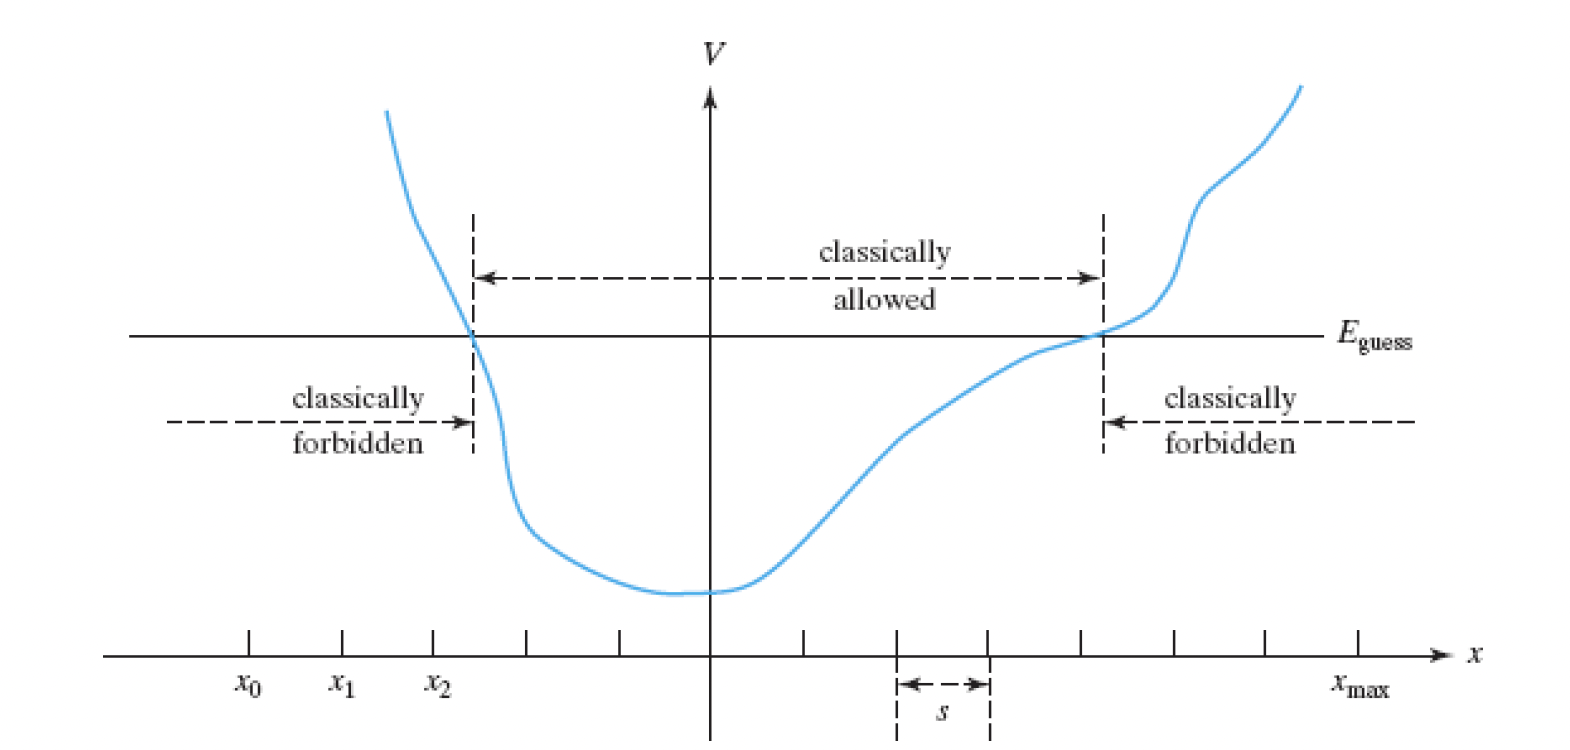
\includegraphics[width=0.8\textwidth]{figures/4.7.png}
        \caption{一维单粒子系统的$V$关于$x$的图象}
        \label{fig:4.7}
    \end{figure}
    
    用涉及$s$的幂的Taylor级数展开$\psi\left(x_n+s\right)$和$\psi\left(x_n-s\right)$,将两式相加即可消去$s$的奇次幂项,并用薛定谔方程来表示 $\psi^{\prime\prime}$ 和 $\psi^{\left(\mathrm{iv}\right)}$,以 $\psi$ 表示,并忽略 $s^6$ 和 $s$ 的高次幂项(如果 $s$ 较小,近似值将是准确的),我们会发现(问题 4.43)
    \begin{equation}
        \psi_{n+1} \equiv = \frac{
            2\psi_n - \psi_{n-1} + 5G_n\psi_n s^2/6 + G_{n-1}\psi_{n-1}s^2/12
        }{
            1-G_{n+1}s^2/12
        }
        \label{eq:4.67}
    \end{equation}
    其中$G_n \equiv G\left(x_n\right) \equiv m\hbar^{-2}\left[2V\left(x_n\right)-2E\right]$[式(\ref{eq:4.66})和\ref{eq:4.65}]。如果知道$\psi_n$和$\psi_{n-1}$,即$\psi$在$x_n$和$x_n-s$处的值,方程(\ref{eq:4.67})允许我们计算$\psi_{n+1}$,即$\psi$在点$x_{n+s}$处的值。

    我们如何使用式(\ref{eq:4.67})来求解薛定谔方程?我们首先猜测一个能量本征值$E_{guess}$。我们从左侧经典禁区(图 \ref{fig:4.7})中的一点 $x_0$ 开始,此处$\psi$的值很小,我们假设$\psi$在该点处的值为零:$\psi_0 \equiv \psi\left(x_0\right) = 0$。同样地,我们也在经典禁区(此处$\psi$的值也很小)的右侧点 $x_{max}$ 处假设 $\psi\left(x_{max}\right)$ 的值为零。我们为连续点之间的间隔 $s$ 选取一个较小的数值,在$x_0+s$处,我们将$\psi$的值设为一个较小的数值,例如0.0001:$\psi_1 \equiv \psi\left(x_1\right) \equiv \psi\left(x_0+s\right) = 0.0001$。$\psi_1$ 的值对找到的本征值不会有任何影响。如果我们令$\psi_1$为0.001,而不是0.0001,公式 (\ref{eq:4.67}) 表明,这只需将后续点上的所有 $\psi$ 值乘以 10 即可(问题 4.41)。这不会影响本征值[见公式 (\ref{eq:3.14 definition of eigenfunctions and eigenvalues}) 后的示例]。在找到每个本征值后,可以对波函数进行归一化处理。
    \begin{figure}[ht]
        \centering
        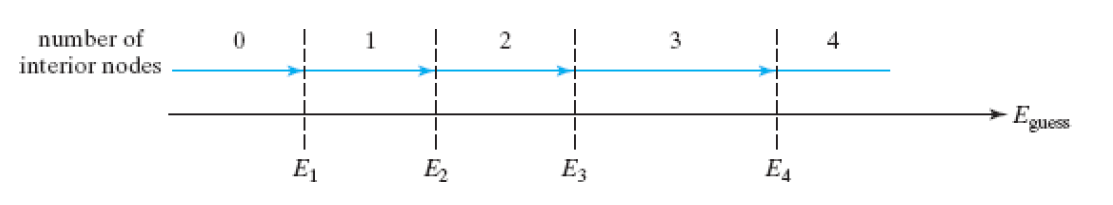
\includegraphics[width=0.8\textwidth]{Figures/4.8.png}
        \caption{Numerov 方法求解的节点数与能量 $E_{guess}$ 的函数关系。}
        \label{fig:4.8}
    \end{figure}

    现在我们有了 $\psi_0$ 和 $\psi_1$ 的值,可以使用式 (\ref{eq:4.67}) 计算 $\psi_2 \equiv \psi\left(x_2\right) \equiv \psi\left(x_1+2s\right)$ 的值,其中我们用$E_{guess}$计算得到$G$的值。接着,在式(\ref{eq:4.67})令$n=2$,我们可以计算出$\psi_3$的值,以此类推,直到达到$x_{max}$。如果$E_{guess}$不等于或不非常接近于本征值,那么$\psi$将不满足平方可积的要求,且$\left|\psi\left(x_{max}\right)\right|$的值会变得非常大。如果发现$\left|\psi\left(x_{max}\right)\right|$不接近于零,那我们重新选一个$E_{guess}$,并从$x_0$开始重复上述过程。这个过程将会循环往复,直到找到能使$\left|\psi\left(x_{max}\right)\right|$非常接近于零的$E_{guess}$的值。此时的$E_{guess}$基本上等同于一个本征值。找到本征值的系统方法是计算由 $E_{guess}$ 生成的 $\psi$ 中的节点。回忆在一维问题中(第\ref{sec:4.2 The One-Dimensional Harmonic Oscillator}节),基态的内部节点数为 0,第一激发态的内部节点数为 1,以此类推。令$E_1,E_2,E_3,\cdots$分别表示基态、第一激发态和第二激发态等的能量值。如果$\psi_{guess}$在$x_0$和$x_{max}$之间没有节点,那么$E_{guess}$应该小于或等于$E_1$。如果$\psi_{guess}$在$x_0$和$x_{max}$之间有一个节点,那么$E_{guess}$应该位于$E_1$和$E_2$之间。随后将给出例子。

\subsection*{无量纲变量}
    Numerov方法需要我们猜测$E$的值。但是我们猜测的数量级:$10^{-20} \: \mathrm{J},10^{-15} \: \mathrm{J},\cdots$应该是多少?为了回答这个问题,我们以谐振子为例,用无量纲变量重表示薛定谔方程。

    谐振子的势能函数为$V = \frac{1}{2}kx^2$,其薛定谔方程包含三个常数,$k$、$m$和$\hbar$。我们试图找到无量纲约化能量 $E_r$ 和无量纲约化 $x$ 坐标 $x_r$,它们的定义是
    \begin{equation}
        E_r \equiv E/A, \quad x_r \equiv x/B
        \label{eq:4.68}
    \end{equation}
    其中常数$A$是$k$、$m$和$\hbar$的组合,具有能量的量纲,而$B$是具有长度量纲的组合。能量的量纲为$\text{质量}\times\text{长度}^2\times\text{时间}^{-2}$,我们写作
    \begin{equation}
        \left[E\right] = \mathrm{M}\mathrm{L}^2\mathrm{T}^{-2}
        \label{eq:4.69}
    \end{equation}
    其中,$E$ 的括号表示其维度,$\mathrm{M}$、$\mathrm{L}$ 和 $\mathrm{T}$ 分别表示质量、长度和时间。方程$V = \frac{1}{2}kx^2$表明$k$的量纲为$\text{能量}\times\text{长度}^{-2}$,由式(\ref{eq:4.69}),有$\left[k\right] = \mathrm{M}\mathrm{T}^{-2}$。$\hbar$的量纲为$\text{能量}\times\text{时间}$。因此,
    \begin{equation}
        \left[m\right] = \mathrm{M}, \quad \left[k\right] = \mathrm{M}\mathrm{T}^{-2}, \quad \left[\hbar\right] = \mathrm{M}\mathrm{L}^2\mathrm{T}^{-1}
        \label{eq:4.70}
    \end{equation}
    式(\ref{eq:4.68})中的$A$和$B$的量纲分别为能量和长度,则
    \begin{equation}
        \left[A\right] = \mathrm{M}\mathrm{L}^2\mathrm{T}^{-2}, \quad \left[B\right] = \mathrm{L}
        \label{eq:4.71}
    \end{equation}

    令$A = m^ak^b\hbar^c$,其中$a$、$b$和$c$是待定的指数,由$A$的量纲一定为$\mathrm{M}\mathrm{L}^2\mathrm{T}^{-2}$所确定。我们有
    \begin{equation}
        \left[A\right] = \left[m^ak^b\hbar^c\right] = \mathrm{M}^a\left(\mathrm{M}\mathrm{T}^{-2}\right)^b\left(\mathrm{M}\mathrm{L}^2\mathrm{T}^{-1}\right)^c = \mathrm{M}^{a+b+c}\mathrm{L}^{2c}\mathrm{T}^{-2b-c}
        \label{eq:4.72}
    \end{equation}
    令 (\ref{eq:4.71}) 和 (\ref{eq:4.72}) 中 M、L 和 T 的指数相等,得到
    \begin{equation*}
        a+b+c = 1, \quad 2c = 2, \quad -2b-c = -2
    \end{equation*}
    解这个方程组,得到$c=1$,$b=\frac{1}{2}$,$a=-\frac{1}{2}$。因此
    \begin{equation}
        A = m^{-1/2}k^{1/2}\hbar
        \label{eq:4.73}
    \end{equation}

    同样地,令$B = m^dk^e\hbar^f$。用得出式(\ref{eq:4.73})相同的量纲分析法,有(问题4.44)
    \begin{equation}
        B = m^{-1/4}k^{-1/4}\hbar^{1/2}
        \label{eq:4.74}
    \end{equation}

    根据式(\ref{eq:4.68})、(\ref{eq:4.73})和(\ref{eq:4.74}),谐振子的约化变量为
    \begin{equation}
        E_r = E / m^{-1/2}k^{1/2}\hbar, \quad x_r = x / m^{-1/4}k^{-1/4}\hbar^{1/2}
        \label{eq:4.75}
    \end{equation}
    使用$k^{1/2} = 2\pi\nu m^{1/2}$[式(\ref{eq:4.23})]将$k$从(\ref{eq:4.75})中消去,并回忆$\alpha \equiv 2\pi\nu m/\hbar$[式(\ref{eq:4.31})],我们得到以下备选的表达式
    \begin{equation}
        E_r = E /h\nu, \quad x_r = \alpha ^{1/2}x
        \label{eq:4.76}
    \end{equation}

    与方程$E_r \equiv E/A$[式(\ref{eq:4.68})]类似,我们可以定义约化势能函数$V_r$:
    \begin{equation}
        V_r \equiv V / A
        \label{eq:4.77}
    \end{equation}

    由于$\left|\psi\left(x\right)\right|^2\mathrm{d}x$是概率,概率是没有量纲的,归一化后的$\psi\left(x\right)$一定具有$\text{长度}^{-1/2}$的量纲。因此,我们可以定义一个没有量纲的约化波函数$\psi_r$。由式(\ref{eq:4.71}),$B$具有长度的量纲,则$B^{-1/2}$具有$\text{长度}^{-1/2}$的量纲。因此,
    \begin{equation}
        \psi_r = \psi / B^{-1/2}
        \label{eq:4.78}
    \end{equation}
    $\psi_r$ 满足 $\int_{-\infty}^{\infty} \left|\psi_r\right|^2\mathrm{d}x_r = 1$;这是由式(\ref{eq:4.76})、 (\ref{eq:4.78}) 和$\int_{-\infty}^{\infty} \left|\psi\right|^2\mathrm{d}x = 1$得出的。

    我们现在使用无量纲变量$E_r$、$x_r$和$\psi_r$来重写薛定谔方程。有
    \begin{equation*}
        \frac{\mathrm{d}^2\psi}{\mathrm{d}x^2} = \frac{\mathrm{d}^2}{\mathrm{d}x^2}B^{-1/2}\psi_r = B^{-1/2}\frac{\mathrm{d}}{\mathrm{d}x}\frac{\mathrm{d}\psi_r}{\mathrm{d}x} = B^{-1/2}\frac{\mathrm{d}}{\mathrm{d}x}\frac{\mathrm{d}\psi_r}{\mathrm{d}x_r}\frac{\mathrm{d}x_r}{\mathrm{d}x} = B^{-1/2}\frac{\mathrm{d}\left(\mathrm{d}\psi_r/\mathrm{d}x_r\right)}{\mathrm{d}x_r}\frac{\mathrm{d}x_r}{\mathrm{d}x}\frac{\mathrm{d}x_r}{\mathrm{d}x}
    \end{equation*}
    \begin{equation}
        \frac{\mathrm{d}^2\psi}{\mathrm{d}x^2} = B^{-5/2}\frac{\mathrm{d}^2\psi_r}{\mathrm{d}x_r^2}
        \label{eq:4.79}
    \end{equation}
    其中,我们用到了$\mathrm{d}x_r/\mathrm{d}x = B^{-1/2}$。将式(\ref{eq:4.68})、(\ref{eq:4.77})和(\ref{eq:4.79})代入薛定谔方程$-\left(\hbar^2/m\right)\left(\mathrm{d}^2\psi/\mathrm{d}x^2\right) + V\psi = E\psi$,得到
    \begin{equation*}
        -\frac{\hbar^2}{m}B^{-5/2}\frac{\mathrm{d}^2\psi_r}{\mathrm{d}x_r^2} + AV_rB^{-1/2}\psi_r = AE_rB^{-1/2}\psi_r
    \end{equation*}
    \begin{equation}
        -\frac{\hbar^2}{2m}\frac{1}{AB^2}\frac{\mathrm{d}^2\psi_r}{\mathrm{d}x_r^2} + V_r\psi_r = E_r\psi_r
        \label{eq:4.80}
    \end{equation}
    根据式(\ref{eq:4.73})和(\ref{eq:4.74}),有$AB^2 = \hbar^2/m$,所以对于谐振子,有$\hbar^2/mAB^2 = 1$。

    更一般地说,让 $V$ 包含一个非无量纲参数 $c$。例如,我们有$V = cx^4$或$V = cx^2\left(1+0.05m^{1/2}c^{1/2}\hbar^{-1}x^2\right)$(注意 $m^{1/2}c^{1/2}\hbar^{-1}x^2$ 是无量纲的,因为 1 是无量纲的,所以它必须是无量纲的)。式(\ref{eq:4.80})中的$AB$一定可以写成$\hbar^rm^sc^t$的形式,其中$r$、$s$和$t$是待定的指数。由于(\ref{eq:4.80})中的$V_r\psi_r$是无量纲的,因此第一项也是无量纲的。那么$\hbar^2/mAB^2$是无量纲的,$AB^2$与$\hbar^2/m$具有相同的量纲。所以$r=2$,$s=1$,$t=0$。因此,$AB^2 = \hbar^2/m$,带入(\ref{eq:4.80}),有无量纲的薛定谔方程
    \begin{equation}
        \frac{\mathrm{d}^2\psi}{\mathrm{d}x_r^2} = \left(2V_r-2E_r\right)\psi_r
        \label{eq:4.81}
    \end{equation}
    \begin{equation}
        \psi^{\prime\prime} = G_r\psi_r, \quad \text{其中} \quad G_r \equiv 2V_r-2E_r
        \label{eq:4.82}
    \end{equation}
    对于谐振子,$V_r \equiv V/A = \frac{1}{2}kx^2/m^{-1/2}k^{1/2}\hbar = \frac{1}{2}x_r^2$,因此[式(\ref{eq:4.73})和式(\ref{eq:4.75})]:
    \begin{equation}
        V_r = \frac{1}{2}x_r^2
        \label{eq:4.83}
    \end{equation}

    将谐振子薛定谔方程约化为只涉及无量纲量的形式 (\ref{eq:4.81})后,我们可以预期最低能量本征值的数量级为 1。

    约化谐振子薛定谔方程(\ref{eq:4.82})与(\ref{eq:4.66})具有相同的形式,所以我们可以用Numerov公式(\ref{eq:4.67})来求解。使用$\psi_r$的值代替$\psi$,$G_r$的值代替$G$,与(\ref{eq:4.68})类似,$s_r$的值代替$s$。

    一旦找到约化能量$E_r$的数值,就可以根据 (\ref{eq:4.75}) 或 (\ref{eq:4.76}) 求出能量 $E$。

\subsection*{$x_r$、$x_0$ 、 $x_{max}$ 和$s_r$的选择}
    我们需要选择$x_r$的起始值、结束值,以及相邻点之间的间隔值$s_r$。假设我们希望找到满足$E_r \le 5$的谐振子的所有本征函数和本征值。我们从左侧经典禁区开始求解,因此首先要找到 $E_r=5$ 的经典禁区。经典允许和经典禁止区域的边界满足$E_r=V_r$。由式(\ref{eq:4.83}),有$V_r = \frac{1}{2}x_r^2$,因此$E_r=V_r$变成了$5=\frac{1}{2}x_r^2$所以满足$E_r \le 5$的经典允许区域为$x_r = -\left(10\right)^{1/2}=-3.16$到$x_r = \left(10\right)^{1/2}=3.16$。若$E_r<5$,则经典允许区域将更小。我们希望从左侧经典禁区($\psi$ 非常小)内的某一点开始求解,我们希望在右侧经典禁区内的某一点结束求解。对于$E_r=5$,左侧的经典禁区在$x_r=-3.16$处结束,,所以一个合理的选择为$x_r=-5$[太深入经典禁区有时会带来麻烦(见下文),因此在选择起点时可能需要试错]。由于 $V$ 是对称的,因此我们将在 $x_r=5$ 处结束求解。

    为了达到合理的精确度,通常至少需要 100 个点,因此我们取 $s_r=0.1$ 以得到 100 个点。从 Numerov 方法的推导中可以看出,$s_r$ 必须很小。合理的规则可能是 $s_r$ 不大于 0.1。
    \begin{quote}
        \small
        \noindent
        如果像通常情况那样,当$x \to \pm \infty$时有$V \to \infty$,那么在经典禁区内起步太远会使 Numerov 公式 (\ref{eq:4.67}) 中的分母 $1-G_{n+1}s^2/12$ 变成负数。我们有 $G_r=2V_r-2E_r$,如果我们从 $V_r$ 非常大的点 $x_0$ 开始,该点的 $G_r$ 可能大到足以使 Numerov 公式的分母为负。这样,该方法就会失效。我们将 $\psi_0$ 取为零,将 $\psi_1$ 取为正数。Numerov 公式 (\ref{eq:4.67}) 表明,如果分母是负数,那么 $\psi_2$ 也将是负数,我们将在 $x_1$ 和 $x_2$ 之间产生一个虚假的 $\psi$ 节点。为了避免这个问题,我们可以减小步长 $s_r$ 或 $x_r$、$x_{max}$、$-x_r$和$-x_0$。(见问题 4.46)。
    \end{quote}

\subsection*{Numerov方法的计算机程序}

\subsection*{使用电子表格求解一维薛定谔方程}

\subsection*{Numerov 方法步骤摘要}






    



\section*{总结}

\section*{习题}

	
	% ===== CHAPTER 5 =====
\chapter{角动量}
\label{chap:5}
\section{同时确定多个属性}
\label{sec:5.1 Simultaneous Specification of Several Properties}
    在本章中,我们将讨论角动量,在下一章中,我们将证明对于氢原子的静止态,电子角动量的大小是恒定的。首先,我们要考虑用什么标准来决定一个系统的哪些性质可以同时赋予定值。

    在第\ref{sec:3.3 Operators and Quantum Mechanics}节中,我们假设:若态函数$\Psi$时算符$\hat{A}$的本征函数,本征值为$s$,则对物理量$A$的测量结果一定为为$s$。若$\Psi$同时是$\hat{A}$和$\hat{B}$的本征函数,即$\hat{A}\Psi=s\Psi$,$\hat{B}\Psi=t\Psi$,那么我们就可以同时为物理量 $A$ 和 $B$ 赋以确定的值。什么时候$\Psi$会同时是两个算符的本征函数呢?在第\ref{chap:7}章中,我们将证明如下两个理论。首先,两个算符的同时本征函数的完整集合存在的必要条件是算符之间可对易(这里使用的“\textit{完整}”一词有一定的技术含义,我们将在第 \ref{chap:7} 章再讨论这个问题)。反之亦然,若对应于物理量的两个算符$\hat{A}$ 和 $\hat{B}$ 可对易,则存在一组完整的函数,它们同时是$\hat{A}$和$\hat{B}$的本征函数。因此,若$\left[\hat{A},\hat{B}\right]=0$,那么$\Psi$可以同时是$\hat{A}$和$\hat{B}$的本征函数。

    回忆算符$\hat{A}$和$\hat{B}$的交换子为$\left[\hat{A},\hat{B}\right] \equiv \hat{A}\hat{B} - \hat{B}\hat{A}$[式(\ref{eq:3.7 definition of commutator for two operators})]。下列等式有助于计算交换子。通过详细写出交换子可以证明这些等式(问题5.2):
    \begin{equation}
        \boxed{
            \left[\hat{A},\hat{B}\right] = -\left[\hat{B},\hat{A}\right]
        }
        \label{eq:5.1}
    \end{equation}
    \begin{equation}
        \boxed{
            \left[\hat{A}, \hat{A}^n\right] = 0, \quad n = 1, 2, 3, \ldots
        }
        \label{eq:5.2}
    \end{equation}
    \begin{equation}
        \boxed{
            \left[k\hat{A},\hat{B}\right] = \left[\hat{A}, k\hat{B}\right] = k\left[\hat{A},\hat{B}\right]
        }
        \label{eq:5.3}
    \end{equation}
    \begin{equation}
        \boxed{
            \left[\hat{A}, \hat{B}+\hat{C}\right] = \left[\hat{A},\hat{B}\right] + \left[\hat{A},\hat{C}\right]
        }
        \quad 
        \boxed{
            \left[\hat{A}+\hat{B},\hat{C}\right] = \left[\hat{A},\hat{C}\right] + \left[\hat{B},\hat{C}\right]
        }
        \label{eq:5.4}
    \end{equation}
    \begin{equation}
        \boxed{
            \left[\hat{A}, \hat{B}\hat{C}\right] = \left[\hat{A},\hat{B}\right]\hat{C} + \hat{B}\left[\hat{A},\hat{C}\right]
        }
        \quad
        \boxed{
            \left[\hat{A}\hat{B},\hat{C}\right] = \hat{A}\left[\hat{B},\hat{C}\right] + \left[\hat{A},\hat{C}\right]\hat{B}
        }
        \label{eq:5.5}
    \end{equation}
    其中$k$是常数,所有算符都假设为线性算符。
    \begin{examplebox}
        \textbf{例题:}从$\left[\partial/\partial x,x\right]=1$[式(\ref{eq:3.8})]出发,使用对易子的性质(式(\ref{eq:5.1})至(\ref{eq:5.5}))求以下对易子:(a)$\left[\hat{x},\hat{p_x}\right]$;(b)$\left[\hat{x}, \hat{p_x^2}\right]$;(c)三维单粒子系统的$\left[\hat{x},\hat{H}\right]$。
        \\
        (a)使用式(\ref{eq:5.3})和(\ref{eq:5.1}),因为$\left[\partial/\partial x,x\right]=1$,我们有
        \begin{equation*}
            \left[\hat{x},\hat{p_x}\right] = \left[\hat{x},\frac{\hbar}{\mathrm{i}}\frac{\partial}{\partial x}\right] = \frac{\hbar}{\mathrm{i}}\left[\hat{x},\frac{\partial}{\partial x}\right] = -\frac{\hbar}{\mathrm{i}}\left[\frac{\partial}{\partial x},\hat{x}\right] = -\frac{\hbar}{\mathrm{i}}
        \end{equation*}
        \begin{equation}
            \left[\hat{x},\hat{p_x}\right]=\mathrm{i}\hbar
            \label{eq:5.6}
        \end{equation}
        (b)由式(\ref{eq:5.5})和(\ref{eq:5.6}),有
        \begin{equation*}
            \left[\hat{x},\hat{p_x^2}\right] = \left[\hat{x},\hat{p_x}\right]\hat{p_x} + \hat{p_x}\left[\hat{x},\hat{p_x}\right] = \mathrm{i}\hbar\cdot\frac{\hbar}{\mathrm{i}}\frac{\partial}{\partial x} + \frac{\hbar}{\mathrm{i}}\frac{\partial}{\partial x} \cdot \mathrm{i}\hbar
        \end{equation*}
        \begin{equation}
            \left[\hat{x},\hat{p_x^2}\right] = 2\hbar^2\frac{\partial}{\partial x}
            \label{eq:5.7}
        \end{equation}
        (c)使用式(\ref{eq:5.4})、(\ref{eq:5.3})和(\ref{eq:5.7}),有
        \begin{equation*}
            \begin{aligned}
                \left[\hat{x},\hat{H}\right] &= \left[\hat{x},\hat{T}+\hat{V}\right] = \left[\hat{x},\hat{T}\right] + \left[\hat{x},\hat{V}\left(x,y,z\right)\right] =\left[\hat{x},\hat{T}\right] \\
                &= \left[\hat{x}, \left(1/2m\right)\left(\hat{p_x^2}+\hat{p_y^2}+\hat{p_z^2}\right)\right]\\
                &= \left(1/2m\right)\left[\hat{x},\hat{p_x^2}\right] + \left(1/2m\right)\left[\hat{x},\hat{p_y^2}\right] + \left(1/2m\right)\left[\hat{x},\hat{p_z^2}\right]\\
                &= \frac{1}{2m}2\hbar^2\frac{\partial}{\partial x} + 0 + 0
            \end{aligned}
        \end{equation*}
        \begin{equation}
            \left[\hat{x},\hat{H}\right] = \frac{\hbar^2}{m}\frac{\partial}{\partial x} = \frac{\mathrm{i}\hbar}{m}\hat{p_x}
            \label{eq:5.8}
        \end{equation}
        \\
        \textbf{练习:}求证:对于单粒子三维系统,有
        \begin{equation}
            \left[\hat{p_x^2},\hat{H}\right] = -\mathrm{i}\hbar \:\partial V\left(x,y,z\right)/\partial x
            \label{eq:5.9}
        \end{equation}
    \end{examplebox}

    这些对易子有重要的物理影响。由于$\left[\hat{x},\hat{p_x}\right] \neq 0$,我们不能希望态函数同时是$\hat{x}$和$\hat{p_x}$的本征函数。因此,与不确定性原理相符,我们不能同时测定$x$和$p_x$的精确值。由于$\hat{x}$与$\hat{H}$不可对易,我们不能指望同时为能量和 $x$ 坐标赋予确定的值。定态(具有确定的能量)会显示出$x$的各种可能值,观察到各种$x$值的概率由玻恩公设给出。

    对于不是$\hat{A}$的本征函数的态函数$\Psi$,在完全相同的系统中对$A$的测量将得到各种可能的结果。我们需要对观测值 $A_i$ 的分布或离散性进行某种测量。如果 $\langle A \rangle$ 是这些值的平均值,那么每个测量值与平均值的偏差为$A_i - \langle A \rangle$。如果我们对所有偏差求平均值,就会得到零,因为正负偏差会抵消。因此,为了使所有偏差都为正值,我们要将它们平方。偏差平方的平均值称为 $A$ 的\textbf{方差}(variance),在统计学中用 $\sigma^2\left(A\right)$ 表示,在量子力学中用 $\left(\Delta A\right)^2$ 表示:
    \begin{equation}
        \left(\Delta A\right)^2 \equiv \sigma^2\left(A\right) = \langle \left(A - \langle A \rangle\right)^2 \rangle = \int \Psi^{\ast}\left(\hat{A}-\langle A \rangle\right)^2\Psi\mathrm{d}\tau
        \label{eq:5.10}
    \end{equation}
    其中我们用到了平均值的表达式(\ref{eq:3.88})。定义(\ref{eq:5.10})与以下表达式等价(问题5.7):
    \begin{equation}
        \left(\Delta A\right)^2 = \langle A^2 \rangle - \langle A \rangle^2
        \label{eq:5.11}
    \end{equation}

    方差的正平方根称为\textbf{标准差}(standard deviation),用 $\Delta A$ 或$\sigma\left(A\right)$ 表示。标准差是最常用的价差度量,我们将用它来度量属性 $A$ 的 “不确定性”。

    罗伯逊(Robertson)于 1929 年证明,状态函数为 $\Psi$ 的量子力学系统的两个属性的标准偏差的乘积必须满足不等式
    \begin{equation}
        \sigma\left(A\right)\sigma\left(B\right) = \Delta A \Delta B \ge \frac{1}{2}\left|\int \Psi^{\ast}\left[\hat{A},\hat{B}\right]\Psi\mathrm{d}\tau\right|
        \label{eq:5.12}
    \end{equation}
    (\ref{eq:5.12}) 的证明源于量子力学公设,见问题 7.60。如果$\hat{A}$和$\hat{B}$可对易,那么式(\ref{eq:5.12})中的积分为零,则$\Delta A$和$\Delta B$可能都为零,与上文的讨论相符。

    作为式(\ref{eq:5.12})的一个例子,我们使用式(\ref{eq:5.6})、$\left|z_1z_2\right|=\left|z_1\right|\left|z_2\right|$[式(\ref{eq:1.34 properties of product and quotient absolute values})],以及归一化方法:
    \begin{equation*}
        \Delta x \Delta p_x \ge \frac{1}{2}\left|\int \Psi^{\ast}\left[\hat{x},\hat{p_x}\right]\Psi\mathrm{d}\tau\right| = \frac{1}{2}\left|\int \Psi^{\ast}\mathrm{i}\hbar\Psi\mathrm{d}\tau\right| = \frac{1}{2}\hbar\left|\mathrm{i}\right|\left|\int \Psi^{\ast}\Psi\mathrm{d}\tau\right|
    \end{equation*}
    \begin{equation}
        \sigma\left(x\right)\sigma\left(p_x\right) \equiv \Delta x \Delta p_x \ge \frac{1}{2}\hbar
        \label{eq:5.13}
    \end{equation}

    式(\ref{eq:5.13})通常被认为是\textbf{海森堡不确定性原理}(Heisenberg Uncertainty Principle)(第\ref{sec:1.3 The Uncertainty Principle}节)的定量表述。然而,公式 (\ref{eq:5.12}) 和 (\ref{eq:5.13}) 中标准偏差的含义与第 \ref{sec:1.3 The Uncertainty Principle} 节中不确定度的含义截然不同。为了在式(\ref{eq:5.13})中找到$\Delta x$,我们选取大量的系统,每个系统都有相同的状态函数 $\psi$,在每个系统中对 $x$ 进行一次测量。将测得的数据标记为$x_i$,计算$\langle x \rangle$和偏差的平方$\left(x_1-\langle x \rangle\right)^2$。我们求出偏差平方的平均值,得到方差,再取平方根,得到标准偏差$\sigma\left(x\right)\equiv \Delta x$。然后我们再取大量的系统,它们具有与得到$\Delta x$时一致的状态$\Psi$,对每个系统测量一次$p_x$,由这些数据计算出$\Delta p_x$。因此,(\ref{eq:5.13})中的统计量 $\Delta x$ 和 $\Delta p_x$ 不是单个测量的误差,也不是通过同时测量 $x$ 和 $p_x$ 得出的。

    令$\varepsilon\left(x\right)$是对 $x$ 的单次测量的典型误差,令$\eta \left(p_x\right)$是测量 $x$ 时对 $p_x$ 造成的典型干扰。1927 年,海森堡分析了进行位置测量的具体思想实验,得出结论:乘积 $\varepsilon\left(x\right)\eta\left(x\right)$ 的数量级为 $h$ 或更大。海森堡没有给出这些量的精确定义。小泽正直(Masanao Ozawa)将海森堡的关系改写为
    \begin{equation*}
        \varepsilon\left(x\right)\eta\left(p_x\right) \ge \frac{1}{2}\hbar
    \end{equation*}
    其中$\varepsilon\left(x\right)$定义为$x$ 的测量值与理论值的方均根偏差,$\eta\left(p_x\right)$定义为测量 $x$ 所产生的$p_x$变化的方均根偏差。更一般地说,对于任意两个性质,小泽将海森堡不确定性原理写成
    \begin{equation}
        \varepsilon\left(A\right)\eta\left(B\right) \ge \frac{1}{2}\left|\int \Psi^{\ast}\left[\hat{A},\hat{B}\right]\Psi\mathrm{d}\tau\right|
        \label{eq:5.14}
    \end{equation}
    小泽提出的论点是:在某些情况下,海森堡不等式 (\ref{eq:5.14}) 可能被违反。小泽推导出以下关系来取代 (\ref{eq:5.14}) [M. Ozawa, Phys. Ozawa, Phys. Rev. A, 67, 042105 (2003); available at \url{arxiv.org/abs/quant-ph/0207121}]:
    \begin{equation*}
        \varepsilon\left(A\right)\eta\left(B\right) + \varepsilon\left(A\right)\sigma\left(B\right) + \sigma\left(A\right)\eta\left(B\right) \ge \frac{1}{2}\left|\int \Psi^{\ast}\left[\hat{A},\hat{B}\right]\Psi\mathrm{d}\tau\right|
    \end{equation*}
    其中$\sigma\left(A\right)$和$\sigma\left(B\right)$由式(\ref{eq:5.10})给出。2012 年,一项测量中子自旋分量的实验发现:自旋分量不服从海森堡误差-扰动不等式 (\ref{eq:5.14}),但服从小泽不等式[J. Erhart 等,《自然物理学》,8, 185 (2012); \url{arxiv.org/abs/1201.1833}]。

    另一个不等式是海森堡不确定关系,即用一台仪器同时测量 $A$ 和 $B$ 的两种性质:
    \begin{equation*}
        \varepsilon\left(A\right)\varepsilon\left(B\right) \ge \frac{1}{2}\left|\int \Psi^{\ast}\left[\hat{A},\hat{B}\right]\Psi\mathrm{d}\tau\right|
    \end{equation*}
    其中$\varepsilon\left(A\right)$和$\varepsilon\left(B\right)$分别是测量$A$与$B$时的实验误差。这一关系已被证明是成立的,前提是某个可信的假设(相信对目前所有可用的测量设备都是成立的)成立(见上文引用的小泽论文参考文献 6-12)。
    \begin{examplebox}
        \textbf{例题:}式 (\ref{eq:3.91}) 、 (\ref{eq:3.92}) 、 (\ref{eq:3.39}) 、 (\ref{eq:3.89}) 之后的等式和问题 3.48 指出:对于单粒子三维系统的基态,有
        \begin{equation*}
            \langle x \rangle = \frac{a}{2}, \quad \langle x^2 \rangle = \left(\frac{1}{3}-\frac{1}{2\pi^2}\right)a^2, \quad \langle p_x \rangle = 0, \quad \langle p_x^2 \rangle = \frac{h^2}{4a^2}
        \end{equation*}
        使用这些结果证明该系统是否遵守不确定性原理(\ref{eq:5.13})。
        \\ 
        
        我们有
        \begin{equation*}
            \left(\Delta x\right)^2 = \langle x^2 \rangle - \langle x \rangle^2 = \left(\frac{1}{3}-\frac{1}{2\pi^2}\right)a^2 - \frac{a^2}{4} = \frac{\pi^2-6}{12\pi^2}a^2
        \end{equation*}
        \begin{equation*}
            \Delta x = \left(\frac{\pi^2-6}{12}\right)^{1/2}\frac{a}{\pi}
        \end{equation*}
        \begin{equation*}
            \Delta p_x = \langle p_x^2 \rangle - \langle p_x \rangle^2 = \frac{h^2}{4a^2}, \quad \Delta p_x = \frac{h}{2a}
        \end{equation*}
        \begin{equation*}
            \Delta x \Delta p_x = \left(\frac{\pi^2-6}{12}\right)^{1/2}\frac{h}{2\pi} = 0.568\hbar > \frac{1}{2}\hbar
        \end{equation*}
    \end{examplebox}

    还有一种涉及能量和时间的不确定关系:
    \begin{equation}
        \Delta E \Delta t \ge \frac{1}{2}\hbar
        \label{eq:5.15}
    \end{equation}
    一些文章指出:(\ref{eq:5.15}) 是通过将 $\mathrm{i}\hbar \: \partial /\partial t$ 作为能量算符,并乘以 $t$ 作为时间算符而从 (\ref{eq:5.12}) 推导出来的。然而,能量算符是哈密顿$\hat{H}$,而不是 $\mathrm{i}\hbar \: \partial /\partial t$。此外,时间不是一种可观测的参数,而是量子力学中的一个参数。因此,不存在量子力学的时间算符(量子力学中的名词 \textbf{可观测}(observable) 指的是系统的物理可测量属性)。方程 (\ref{eq:5.15}) 必须通过特殊处理才能得出,我们略去不表(见 \textit{Ballentine},第12.3节)。式 (\ref{eq:5.15}) 的推导表明:$\Delta t$被解释为能量不确定度为$\Delta E$的状态的时间寿命。通常情况下,(\ref{eq:5.15})中的 $\Delta t$ 是能量测量的持续时间。然而,Aharonov和Bohm已经证明:“能量可以在任意短的时间内重复测量”[Y. Aharonov and D. Bohm, \textit{Phys. Rev.}, 122, 1649 (1961); 134, B1417 (1964); see also S. Massar and S. Popescu, \textit{Phys. Rev.} A, 71, 042106 (2005); P. Busch, \textit{The Time–Energy Uncertainty Relation}, \url{arxiv.org/abs/quant-ph/0105049}]。

    现在,我们来考虑同时为三个物理量赋予确定值的可能性:假设
    \begin{equation}
        \left[\hat{A},\hat{B}\right] = 0, \quad \left[\hat{A},\hat{C}\right] = 0
        \label{eq:5.16}
    \end{equation}
    这是否足以确保存在三个算符的同时本征函数?由于$\left[\hat{A},\hat{B}\right] = 0$,我们可以为 $\hat{A}$ 和 $\hat{B}$ 构造一组共同的本征函数。由于$\left[\hat{A},\hat{C}\right] = 0$,我们可以为 $\hat{A}$ 和 $\hat{C}$ 构造一组共同的本征函数。如果这两组本征函数是相同的,那么我们就会为所有三个算符找到一组共同的本征函数。因此我们要问:线性算符 $\hat{A}$ 的本征函数集是唯一确定的吗(除了乘以任意常数)?一般来说,答案都是否。如果与 $\hat{A}$ 的本征值相对应的独立本征函数不止一个(即简并),那么简并本征值的本征函数的任何线性组合都是$\hat{A}$ 的本征函数(第 \ref{sec:3.6 Degeneracy} 节)。给出 $\hat{B}$ 本征函数所需的适当线性组合很可能与给出 $\hat{C}$ 本征函数的线性组合不同。事实上,要想拥有三个算符的共同完整的本征函数集,除了满足式(\ref{eq:5.16})外,还需要满足$\left[\hat{B},\hat{C}\right] = 0$。\textit{要有一组完整的函数同时是几个算符的本征函数,每个算符必须与其他每个算符可对易。}

\section{矢量}
\label{sec:5.2 Vectors}
    下一节我们将求解角动量的本征值问题,角动量是一种矢量。因此,我们首先回顾一下矢量。

    完全由大小指定的物理属性(如质量、长度、能量)称为\textbf{标量}(scalar)。需要同时指定大小和方向的物理属性(如力、速度、动量)称为\textbf{矢量}(vector)。矢量由一条有方向的线段表示,其长度和方向表示属性的大小和方向。

    两个矢量 $\mathbf{A}$ 和 $\mathbf{B}$ 的和由如下过程定义:滑动第一个矢量,使其终点与第二个矢量的起点重合,同时保持其方向不变。然后从第二个矢量的尾部到第一个矢量的头部绘制一个新的矢量。参见图 \ref{fig:5.1}。矢量与标量乘积$c\mathbf{A}$定义为:长度为$\left|c\right|$的矢量长度乘以$\mathbf{A}$的长度,若$c$为正,则方向与$\mathbf{A}$相同;若$c$为负,则方向与$\mathbf{A}$相反。
    \begin{figure}[h!]
        \centering
        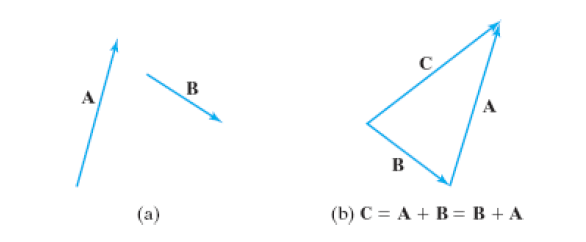
\includegraphics[width=0.7\textwidth]{Figures/5.1.png}
        \caption{两个矢量的和}
        \label{fig:5.1}
    \end{figure}
    \begin{figure}[h!]
        \centering
        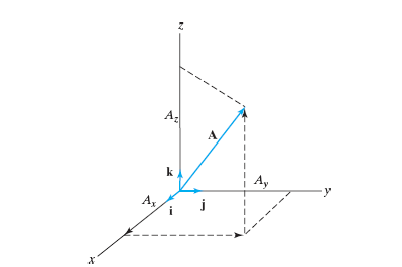
\includegraphics[width=0.7\textwidth]{Figures/5.2.png}
        \caption{单位矢量$\mathrm{i}$、$\mathrm{j}$和$\mathrm{k}$,$\mathrm{A}$的三个分量}
        \label{fig:5.2}
    \end{figure}

    为了获得表示矢量的代数(以及几何)方法,我们在空间中建立了笛卡尔坐标。我们在$x$轴正方向画一个单位矢量,称为$\mathbf{i}$(与虚数单位没有关系)。$y$轴和$z$轴的单位矢量分别称为$\mathbf{j}$和$\mathbf{k}$(图 \ref{fig:5.2})。为了用这三个单位矢量表示空间中的任意矢量$\mathbf{A}$,我们首先将$\mathbf{A}$的起点与原点重合,保持其方向不变。然后,我们找到$\mathbf{A}$在$x$轴、$y$轴和$z$轴上的投影,分别为 $A_x$、$A_y$ 和 $A_z$。由矢量加和的定义,我们有(图 \ref{fig:5.2}):
    \begin{equation}
        \boxed{
            \mathbf{A} = A_x\mathbf{i} + A_y\mathbf{j} + A_z\mathbf{k}
        }
        \label{eq:5.17}
    \end{equation}
    我们可以通过指定$\mathbf{A}$的三个分量($A_x$、$A_y$ 和 $A_z$)来指定矢量 $\mathbf{A}$。因此,三维空间中的矢量可以定义为由三个数组成的有序集合。

    当且仅当两个矢量所有对应的分量都相等时:$A_x = B_x$、$A_y = B_y$ 和 $A_z = B_z$,我们才说这两个向量$\mathbf{A}$和$\mathbf{B}$相等。因此,一个矢量方程等价于三个标量方程。

    为了将两个矢量相加,我们将它们对应的分量相加:
    \begin{equation*}
        \mathbf{A} + \mathbf{B} = A_x\mathbf{i} + A_y\mathbf{j} + A_z\mathbf{k} + B_x\mathbf{i} + B_y\mathbf{j} + B_z\mathbf{k}
    \end{equation*}
    \begin{equation}
        \boxed{
            \mathbf{A} + \mathbf{B} = (A_x + B_x)\mathbf{i} + (A_y + B_y)\mathbf{j} + (A_z + B_z)\mathbf{k}
        }
        \label{eq:5.18}
    \end{equation}
    若$c$是标量,则
    \begin{equation}
        \boxed{
            c\mathbf{A} = cA_x\mathbf{i} + cA_y\mathbf{j} + cA_z\mathbf{k}
        }
        \label{eq:5.19}
    \end{equation}

    矢量$\mathbf{A}$的\textbf{模}(magnitude)为它的长度,由$A$或$\left|\mathbf{A}\right|$表示。模$A$是一个标量。

    两个矢量$\mathbf{A}\cdot\mathbf{B}$的\textbf{点积}(dot product)或\textit{数量积}(scalar product)定义为
    \begin{equation}
        \boxed{
            \mathbf{A}\cdot\mathbf{B} = \left|A\right|\left|B\right|\cos\theta = \mathbf{B}\cdot\mathbf{A}
        }
        \label{eq:5.20}
    \end{equation}
    其中$\theta$是$\mathbf{A}$和$\mathbf{B}$之间的夹角。点积是三个标量的乘积,因此是一个标量。注意$\left|\mathbf{A}\right|\cos\theta$是$\mathbf{A}$在$\mathbf{B}$方向上的投影。根据矢量加法的定义,可以得出矢量 $\mathbf{A}$ + $\mathbf{B}$ 在某个矢量 $\mathbf{C}$ 上的投影是 $\mathbf{A}$ 和 $\mathbf{B}$ 在 $\mathbf{C}$ 上的投影之和。因此,
    \begin{equation}
        \left(\mathbf{A} + \mathbf{B}\right)\cdot\mathbf{C} = \left(\mathbf{A}\cdot\mathbf{C}\right) + \left(\mathbf{B}\cdot\mathbf{C}\right)
        \label{eq:5.21}
    \end{equation}
    由于三个单位矢量 $\mathbf{i}$、$\mathbf{j}$ 和 $\mathbf{k}$ 的长度均为单位长度且互相垂直,我们有
    \begin{equation}
        \mathbf{i}\cdot\mathbf{i} = \mathbf{j}\cdot\mathbf{j} = \mathbf{k}\cdot\mathbf{k} = \cos 0 = 1, \quad \mathbf{i}\cdot\mathbf{j} = \mathbf{i}\cdot\mathbf{k} = \mathbf{j}\cdot\mathbf{k} = \cos \left(\pi/2\right) = 0
        \label{eq:5.22}
    \end{equation}

    使用(\ref{eq:5.22})和分配律(\ref{eq:5.21}),我们有
    \begin{equation*}
        \mathbf{A}\cdot\mathbf{B} = \left(A_x\mathbf{i} + A_y\mathbf{j} + A_z\mathbf{k}\right)\cdot\left(B_x\mathbf{i} + B_y\mathbf{j} + B_z\mathbf{k}\right)
    \end{equation*}
    \begin{equation}
        \boxed{
            \mathbf{A}\cdot\mathbf{B} = A_xB_x + A_yB_y + A_zB_z
        }
        \label{eq:5.23}
    \end{equation}
    其中点积的 9 项中有 6 项为零。

    由式(\ref{eq:5.20})有
    \begin{equation}
        \boxed{
            \mathbf{A}\cdot\mathbf{A} = \left|\mathbf{A}\right|^2
        }
        \label{eq:5.24}
    \end{equation}
    使用式(\ref{eq:5.23}),我们有
    \begin{equation}
        \boxed{
            \left|\mathbf{A}\right| = \left(A_x^2 + A_y^2 + A_z^2\right)^{1/2}
        }
        \label{eq:5.25}
    \end{equation}

    对于三维矢量,还有另一种乘积方式。$\mathbf{A}\times\mathbf{B}$的\textbf{叉积}(cross product)或\textit{向量积}(vector product)是一个新的矢量,其模为
    \begin{equation}
        \mathbf{A}\times\mathbf{B} = \left|\mathbf{A}\right|\left|\mathbf{B}\right|\sin\theta
        \label{eq:5.26}
    \end{equation}
    其线段垂直于$\mathbf{A}$和$\mathbf{B}$所在的平面,其方向与$\mathbf{A}$和$\mathbf{B}$形成一个右手定则的系统(与$x$轴、$y$轴和$z$轴的右手定则相同)。见图 \ref{fig:5.3}。因此,由定义,我们有
    \begin{equation*}
        \mathbf{B}\times\mathbf{A} = -\mathbf{A}\times\mathbf{B}
    \end{equation*}
    同样地(见\textit{Taylor and Mann}, Section 10.2)
    \begin{equation}
        \mathbf{A}\times\left(\mathbf{B}+\mathbf{C}\right) = \mathbf{A}\times\mathbf{B} + \mathbf{A}\times\mathbf{C}
        \label{eq:5.27}
    \end{equation}
    \begin{figure}[h!]
        \centering
        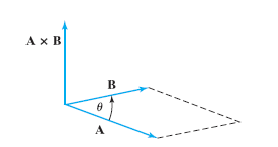
\includegraphics[width=0.4\textwidth]{Figures/5.3.png}
        \caption{两个矢量的叉积}
        \label{fig:5.3}
    \end{figure}
    对于三个单位向量,我们有
    \begin{equation*}
        \mathbf{i}\times\mathbf{i} = \mathbf{j}\times\mathbf{j} = \mathbf{k}\times\mathbf{k} = \sin \: 0 = 0
    \end{equation*}
    \begin{equation*}
        \mathbf{i}\times\mathbf{j} = \mathbf{k}, \quad \mathbf{j}\times\mathbf{i} = -\mathbf{k}, \quad \mathbf{j}\times\mathbf{k} = \mathbf{i}, \quad \mathbf{k}\times\mathbf{j} = -\mathbf{i}, \quad \mathbf{k}\times\mathbf{i} = \mathbf{j}, \quad \mathbf{i}\times\mathbf{k} = -\mathbf{j}
    \end{equation*}
    使用这些等式及分配律(\ref{eq:5.27}),我们有
    \begin{equation*}
        \mathbf{A}\times\mathbf{B} = \left(A_x\mathbf{i} + A_y\mathbf{j} + A_z\mathbf{k}\right)\times\left(B_x\mathbf{i} + B_y\mathbf{j} + B_z\mathbf{k}\right)
    \end{equation*}
    \begin{equation*}
        \mathbf{A}\times\mathbf{B} = \left(A_yB_z - A_zB_y\right)\mathbf{i} + \left(A_zB_x - A_xB_z\right)\mathbf{j} + \left(A_xB_y - A_yB_x\right)\mathbf{k}
    \end{equation*}
    为了便于记忆,我们可以将叉积表示为行列式(见第 8.3 节):
    \begin{equation}
        \mathbf{A}\times\mathbf{B} = \left|
            \begin{array}{ccc}
            \mathbf{i} & \mathbf{j} & \mathbf{k} \\
            A_x & A_y & A_z \\
            B_x & B_y & B_z
            \end{array}
        \right| = \mathbf{i}\left|
            \begin{array}{ccc}
            A_y & A_z \\
            B_y & B_z
            \end{array}
        \right| - \mathbf{j}\left|
            \begin{array}{ccc}
            A_x & A_z \\
            B_x & B_z
            \end{array}
        \right| + \mathbf{k}\left|
            \begin{array}{ccc}
            A_x & A_y \\
            B_x & B_y
            \end{array}
        \right|
        \label{eq:5.28}
    \end{equation}

    我们定义如下的矢量\textbf{微分}(del)算符:
    \begin{equation}
        \boxed{
            \nabla \equiv \mathbf{i}\frac{\partial}{\partial x} + \mathbf{j}\frac{\partial}{\partial y} + \mathbf{k}\frac{\partial}{\partial z}
        }
        \label{eq:5.29}
    \end{equation}
    则由式(\ref{eq:3.23}),线性动量的矢量算符为$\hat{\mathbf{p}}=-\mathrm{i}\hbar\nabla$。

    函数$g\left(x,y,z\right)$的\textbf{梯度}(gradient)定义为将微分算符作用到函数$g$上的结果:
    \begin{equation}
        \boxed{
            \mathbf{grad} \: g\left(x,y,z\right) \equiv \nabla g\left(x,y,z\right) \equiv \mathbf{i}\frac{\partial g}{\partial x} + \mathbf{j}\frac{\partial g}{\partial y} + \mathbf{k}\frac{\partial g}{\partial z}
        }
        \label{eq:5.30}
    \end{equation}
    一个标量函数的梯度为一个矢量函数。矢量$\nabla g\left(x,y,z\right)$代表函数$g$的空间变化率:$\nabla \:g$在$x$方向的分量表示函数$g$在$x$方向的变化率,以此类推。可以证明,矢量$\nabla g$指向 g 变化率最大的方向。由式(\ref{eq:4.24}),势能和力之间的关系为
    \begin{equation}
        \mathbf{F} = -\nabla V\left(x,y,z\right) = -\mathbf{i}\frac{\partial V}{\partial x} - \mathbf{j}\frac{\partial V}{\partial y} - \mathbf{k}\frac{\partial V}{\partial z}
        \label{eq:5.31}
    \end{equation}

    假设某矢量$\mathbf{A}$的三个分量是某参数$t$的函数,即$A_x = A_x\left(t\right)$、$A_y = A_y\left(t\right)$和$A_z = A_z\left(t\right)$。则我们将$\mathbf{A}$对$t$的\textbf{导数}(derivative)定义为
    \begin{equation}
        \frac{\mathrm{d}\mathbf{A}}{\mathrm{d}t} = \mathbf{i}\frac{\mathrm{d}A_x}{\mathrm{d}t} + \mathbf{j}\frac{\mathrm{d}A_y}{\mathrm{d}t} + \mathbf{k}\frac{\mathrm{d}A_z}{\mathrm{d}t}
        \label{eq:5.32}
    \end{equation}

    矢量符号是表示函数变量的一种便捷方法。双粒子系统的波函数可以写作$\psi\left(x_1,y_1,z_1,x_2,y_2,z_2\right)$,如果矢量$\mathbf{r}_1$从原点指向粒子1,那么$\mathbf{r}_1$就具有$x,y,z$三个方向的分量,指定$\mathbf{r}_1$等同于指定三个坐标$x,y,z$。$\mathbf{r}_2$也是如此。因此,我们可以将波函数写成$\psi\left(\mathbf{r}_1,\mathbf{r}_2\right)$。矢量符号也可以用在积分中,例如式(\ref{eq:3.57})对全空间的积分经常写成$\int \cdots \int\left|\Psi\left(\mathbf{r}_1,\cdots,\mathbf{r}_n\right)\right|^2\mathrm{d}\mathbf{r}_1\cdots\mathrm{d}\mathbf{r}_n$。
    
    
\subsection*{$n$维空间的矢量}

    矢量的定义可以推广到三维以上的空间。三维空间中的矢量$\mathbf{A}$可以由其模$\left|\mathbf{A}\right|$和方向来定义;若在笛卡尔坐标系中,还可以用其三个分量$\left(A_x,A_y,A_z\right)$来定义。因此,我们可以把三维矢量定义为按特定顺序排列的三个实数$\left(A_x,A_y,A_z\right)$的集合。$n$ 维实数矢量 “空间”(有时称为超空间)中的矢量 $\mathbf{B}$ 定义为 $n$ 个实数的有序集合$\left(B_1,B_2,\cdots,B_n\right)$,其中$B_1$,$B_2$,$\cdots$,$B_n$是$\mathbf{B}$的\textbf{分量}(components)。不要担心无法将 $n$ 维空间中的矢量可视化。

    函数的变量通常使用 $n$ 维矢量符号表示。例如,在双粒子系统中,与$\psi\left(x_1,y_1,z_1,x_2,y_2,z_2\right)$不同,我们可以定义一个六维矢量$\mathbf{q}$,其分量满足$q_1=x_1, q_2=y_1, q_3=z_1, q_4=x_2, q_5=y_2, q_6=z_2$,且将波函数写成 $\psi\left(\mathbf{q}\right)$。对于有$n$个粒子的系统,我们可以定义一个有$3n$个分量的矢量$\mathbf{q}$,将波函数写成$\psi\left(\mathbf{q}\right)$,使用$\int\left|\psi\left(\mathbf{q}\right)\right|^2\mathrm{d}\mathbf{q}$来进行归一化处理。

    寻找分子平衡几何的理论使用 $n$ 维矢量(第 \ref{sec:15.10 Molecular Geometry} 节)。第 \ref{sec:5.2 Vectors} 节的其余部分与第 \ref{sec:15.10 Molecular Geometry} 节相关,在学习第 \ref{sec:15.10 Molecular Geometry} 节之前不必阅读。

    当且仅当$n$维矢量$\mathbf{B}$和$\mathbf{C}$的所有分量都相等时:$B_1 = C_1$、$B_2 = C_2$、$\cdots$、$B_n = C_n$,我们才说这两个向量\textbf{相等}(equal)。因此,在$n$维空间中,一个矢量方程等价于 $n$ 个标量方程。两个$n$维矢量$\mathbf{B}$与$\mathbf{D}$\textbf{和}(sum)的定义为矢量$\left(B_1+D_1,B_2+D_2,\cdots,B_n+D_n\right)$。矢量的差定义类似。矢量$k\mathbf{B}$定义为矢量$\left(kB_1,kB_2,\cdots,kB_n\right)$,其中 $k$ 是标量。在三维空间中,若$k>0$,则矢量$k\mathbf{A}$的方向一致。在$n$维空间中亦然。与实数对$\left(A_x,A_y,A_z\right)$定义三维空间中的一个点类似,$\left(B_1,B_2,\cdots,B_n\right)$定义$n$维空间中的一个\textbf{点}(point)。

    $n$ 维实数矢量的\textbf{长度}(length)(或\textbf{大小}(magnitude)或\textbf{欧几里得范数}(Euclidean norm))$\left|\mathbf{B}\right|$(有时表示为$\left|\left|\mathbf{B}\right|\right|$ )定义为
    \begin{equation*}
        \left|\mathbf{B}\right| \equiv \left(\mathbf{B}\cdot\mathbf{B}\right)^{1/2} = \left(B_1^2 + B_2^2 + \cdots + B_n^2\right)^{1/2}
    \end{equation*}
    长度为1的矢量称为\textbf{归一化的}(normalized)。

    两个$n$维矢量$\mathbf{B}$和$\mathbf{G}$的\textbf{内积}(inner product)或\textbf{数量积}(scalar product)定义为标量
    \begin{equation*}
        \mathbf{B}\cdot\mathbf{G} \equiv B_1G_1 + B_2G_2 + \cdots + B_nG_n
    \end{equation*}
    若$\mathbf{B}\cdot\mathbf{G}=0$,则称$\mathbf{B}$和$\mathbf{G}$\textbf{正交}(orthogonal)。由式(\ref{eq:5.20}),两个$n$维矢量夹角$\theta$的余弦值定义为$\cos\theta \equiv \left(\mathbf{B}\cdot\mathbf{C}\right)/\left|\mathbf{B}\right|\left|\mathbf{C}\right|$。我们可以证明,这个定义使得 $\theta$ 位于-1 到 1 的范围内。

    在三维空间内,单位矢量$\mathbf{i} = \left(1,0,0\right), \mathbf{j} = \left(0,1,0\right), \mathbf{k} = \left(0,0,1\right)$互相垂直。因此,任意矢量都可以表示为这三个矢量的线性组合[式(\ref{eq:5.17})]。在$n$维空间中,单位矢量$\mathbf{e}_1 \equiv \left(1,0,\cdots,0\right), \mathbf{e}_2 \equiv \left(0,1,\cdots,0\right), \cdots, \mathbf{e}_n \equiv \left(0,0,\cdots,1\right)$互相正交。由于任意$n$维矢量$\mathbf{B}$等于$B_1\mathbf{e}_1 + B_2\mathbf{e}_2 + \cdots + B_n\mathbf{e}_n$,任意$n$维矢量都可以表示为这$n$个单位矢量的线性组合。因此,这 $n$ 个矢量可以说是 $n$ 维实数矢量空间的\textbf{基}(basis)。由于矢量$\mathbf{e_1}, \mathbf{e}_2, \cdots, \mathbf{e}_n$是正交且归一的,它们是这个实矢量空间的\textbf{正交}基(orthonormal basis)。点积$\mathbf{B}\cdot\mathbf{e_i}$给出了矢量 $\mathbf{B}$ 在 $\mathbf{e}_i$ 方向上的分量。矢量空间有许多可能的基集。任何由 $n$ 个线性无关的实矢量组成的集合都可以作为 $n$ 维实矢量空间的基。

    一个三维矢量可以用它的三个分量来指定,也可以用它的长度和方向来指定。可以通过给出矢量与 $x$、$y$ 和 $z$ 轴正半轴所成的三个角度来指定方向。这些角度称为矢量的\textbf{方向角}(direction angles),其值在$0$到$\pi$之间。但是,一旦给出了其他两个方向角,$z$ 轴的方向角就会固定下来,因此只有两个方向角是独立的。因此,一个三维矢量可以用长度和两个方向角来表示。同样,在$n$维空间中,一个矢量和每个单位矢量$\mathbf{e_1},\mathbf{e_2},\cdots,\mathbf{e_n}$之间的方向角也可以根据上述两个矢量之间夹角的余弦公式求出。因此,一个 $n$ 维矢量可以用它的长度和 $n-1$ 个方向角来指定。

    三变量函数的梯度由 (\ref{eq:5.30}) 定义。$n$变量函数$f\left(q_1,q_2,\cdots,q_n\right)$的\textbf{梯度}(gradient)定义为$n$维矢量,其分量分别为$f$对每个变量的一阶偏导数:
    \begin{equation*}
        \nabla f \equiv \left(\partial f/\partial q_1\right)\mathbf{e_1} + \left(\partial f/\partial q_2\right)\mathbf{e}_2 + \cdots + \left(\partial f/\partial q_n\right)\mathbf{e}_n
    \end{equation*}

    我们考虑的是实数 $n$ 维矢量空间。狄拉克(Dirac)对量子力学的表述使用的是复数、无穷维的矢量空间,对它的讨论从略。

\section{单粒子系统的角动量}
\label{sec:5.3 Angular Momentum of a One-Particle System}
    在第\ref{sec:3.3 Operators and Quantum Mechanics}节中,我们找到了线性动量算符$\hat{p}_x$的本征函数和对应的本征值。本节中我们对粒子的角动量进行类似的分析。角动量在原子结构的量子力学中扮演重要的角色。我们从回顾经典力学的角动量开始。

    \subsection*{单粒子的经典力学角动量}
    考虑一个质量为 $m$ 的运动粒子。我们建立一个固定在空间的直角坐标系。设$\mathbf{r}$为从原点指向粒子瞬时位置的矢量,我们有
    \begin{equation}
        \mathbf{r} = \mathbf{i}x + \mathbf{j}y + \mathbf{k}z
        \label{eq:5.33}
    \end{equation}
    其中$x$、$y$ 和 $z$ 是粒子在给定瞬间的坐标。这些坐标是时间的函数。将速度矢量$\mathbf{v}$定义为粒子位置矢量$\mathbf{r}$对时间的导数,我们有[式(\ref{eq:5.32})]
    \begin{equation}
        \mathbf{v} \equiv \frac{\mathrm{d}\mathbf{r}}{\mathrm{d}t} = \mathbf{i}\frac{\mathrm{d}x}{\mathrm{d}t} + \mathbf{j}\frac{\mathrm{d}y}{\mathrm{d}t} + \mathbf{k}\frac{\mathrm{d}z}{\mathrm{d}t}
        \label{eq:5.34}
    \end{equation}
    \begin{equation*}
        v_x = \mathrm{d}x/\mathrm{d}t, \quad v_y = \mathrm{d}y/\mathrm{d}t, \quad v_z = \mathrm{d}z/\mathrm{d}t
    \end{equation*}

    我们定义粒子的\textbf{线性动量}(linear momentum)的矢量$\mathbf{p}$为
    \begin{equation}
        \boxed{
            \mathbf{p} \equiv m\mathbf{v}
        }
        \label{eq:5.35}
    \end{equation}
    \begin{equation}
        p_x = mv_x, \quad p_y = mv_y, \quad p_z = mv_z
        \label{eq:5.36}
    \end{equation}

    粒子相对于坐标原点的\textbf{角动量}(angular momentum)$\mathbf{L}$在经典力学中定义为
    \begin{equation}
        \boxed{
            \mathbf{L} \equiv \mathbf{r} \times \mathbf{p}
        }
        \label{eq:5.37}
    \end{equation}
    \begin{equation}
        \mathbf{L} = \left|
            \begin{array}{ccc}
            \mathbf{i} & \mathbf{j} & \mathbf{k} \\
            x & y & z \\
            p_x & p_y & p_z
            \end{array}
            \right|
        \label{eq:5.38}
    \end{equation}
    \begin{equation}
        L_x = yp_z - zp_y, \quad L_y = zp_x - xp_z, \quad L_z = xp_y - yp_x
        \label{eq:5.39}
    \end{equation}
    其中,我们用到了式(\ref{eq:5.28})。$L_x$、$L_y$ 和 $L_z$ 分别是角动量矢量 $\mathbf{L}$ 在 $x$、$y$ 和 $z$ 方向上的分量。角动量向量的方向垂直于由粒子的位置矢量$\mathbf{r}$和速度矢量$\mathbf{v}$所确定的平面(图\ref{fig:5.4})。
    \begin{figure}[h!]
        \centering
        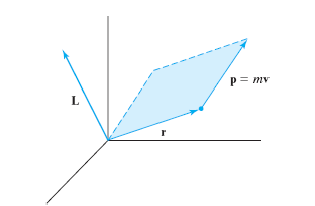
\includegraphics[width=0.5\textwidth]{Figures/5.4.png}
        \caption{$\mathbf{L \equiv \mathbf{r} \times \mathbf{p}}$}
        \label{fig:5.4}
    \end{figure}

    作用在粒子上的\textit{力矩}(torque)$\tau$定义为力$\mathbf{F}$和位置矢量$\mathbf{r}$的叉积:$\tau \equiv \mathbf{r} \times \mathbf{F}$。可以证明:$\tau = \mathrm{d}\mathbf{L} / \mathrm{d}t$。当没有力矩作用于粒子时,其角动量的变化率为零;也就是说,其角动量是恒定的(或守恒的)。对于绕太阳运行的行星来说,引力是沿径向分布的。由于两个平行矢量的交积为零,因此行星上没有力矩,其角动量是守恒的。

\subsection*{单粒子轨道角动量算符}
    现在,让我们来看看量子力学的处理方法。量子力学中有两种角动量。\textbf{轨道角动量}(orbital angular momentum)是粒子在空间运动的结果,与经典力学量 $\mathbf{L}$ 类似。\textbf{自旋角动量}(spin angular momentum)(第\ref{chap:10}章)是许多微观粒子的固有属性,与经典力学没有类似之处。我们现在只考虑轨道角动量。将经典方程(\ref{eq:5.39}) 中的坐标和角动量替换为相应的算符[式 (\ref{eq:3.21})-(\ref{eq:3.23})] ,我们就得到了粒子轨道角动量分量的量子力学算符。有
    \begin{equation}
        \hat{L}_x = -\mathrm{i}\hbar\left(y\frac{\partial}{\partial z} - z\frac{\partial}{\partial y}\right)
        \label{eq:5.40}
    \end{equation}
    \begin{equation}
        \hat{L}_y = -\mathrm{i}\hbar\left(z\frac{\partial}{\partial x} - x\frac{\partial}{\partial z}\right)
        \label{eq:5.41}
    \end{equation}
    \begin{equation}
        \hat{L}_z = -\mathrm{i}\hbar\left(x\frac{\partial}{\partial y} - y\frac{\partial}{\partial x}\right)
        \label{eq:5.42}
    \end{equation}
    (由于$\hat{y}\hat{p}_z = \hat{p}_z\hat{y}$等,我们在构造这些算符时不会遇到不可对易的问题)。使用
    \begin{equation}
        \hat{L}^2 = \left|\hat{\mathbf{L}}\right|^2 = \hat{\mathbf{L}}\cdot\hat{\mathbf{L}} = \hat{L}_x^2 + \hat{L}_y^2 + \hat{L}_z^2
        \label{eq:5.43}
    \end{equation}
    我们可以根据 (\ref{eq:5.40})-(\ref{eq:5.42}) 中的算符构建角动量大小平方的算符。

    由于对易关系决定了哪些物理量可以同时被赋予定值,我们对角动量的对易关系进行了研究。将算符$\hat{L}_y$作用到函数$f\left(x,y,z\right)$上,我们有
    \begin{equation*}
        \hat{L}_yf\left(x,y,z\right) = -\mathrm{i}\hbar\left(z\frac{\partial f}{\partial x} - x\frac{\partial f}{\partial z}\right)
    \end{equation*}
    将$\hat{L}_x$作用到上一个方程上,我们有
    \begin{equation}
        \hat{L}_x\hat{L}_yf = -\hbar^2\left(y\frac{\partial f}{\partial x} + yz \frac{\partial^2f}{\partial z \: \partial x} - yx\frac{\partial^2f}{\partial z^2} - z^2\frac{\partial ^2f}{\partial y \: \partial x} + zx\frac{\partial^2f}{\partial y\: \partial z}\right)
        \label{eq:5.44}
    \end{equation}
    同样地,
    \begin{equation*}
        \hat{L}_xf = -\mathrm{i}\hbar\left(y\frac{\partial f}{\partial z} - z\frac{\partial f}{\partial y}\right)
    \end{equation*}
    将$\hat{L}_y$作用到上一个方程上,我们有
    \begin{equation}
        \hat{L}_y\hat{L}_xf = -\hbar^2\left(zy\frac{\partial^2f}{\partial x\: \partial z}  - z^2\frac{\partial ^2f}{\partial x \: \partial y} - xy\frac{\partial^2f}{\partial z^2} + x\frac{\partial f}{\partial y} + xz \frac{\partial^2f}{\partial z \: \partial y}\right)
        \label{eq:5.45}
    \end{equation}
    (\ref{eq:5.44}) 减去 (\ref{eq:5.45}) ,我们得到
    \begin{equation*}
        \hat{L}_x\hat{L}_yf - \hat{L}_y\hat{L}_xf = -\hbar^2\left(y\frac{\partial f}{\partial x} - x\frac{\partial f}{\partial y}\right)
    \end{equation*}
    \begin{equation}
        \left[\hat{L}_x, \hat{L}_y\right] = \mathrm{i}\hbar\hat{L}_z
        \label{eq:5.46}
    \end{equation}
    其中我们用到了类似以下的关系:
    \begin{equation}
        \boxed{
            \frac{\partial ^2f}{\partial z \: \partial x} = \frac{\partial ^2f}{\partial x \: \partial z}
        }
        \label{eq:5.47}
    \end{equation}
    对于品优函数是正确的。我们可以用相同的过程求出$\left[\hat{L}_y, \hat{L}_z\right]$和$\left[\hat{L}_z, \hat{L}_x\right]$。但我们可以通过注意 (\ref{eq:5.40})-(\ref{eq:5.42}) 中的某种对称性来节省时间。所谓$x$、$y$和$z$的\textbf{循环排列}(cyclic permutation)是指用$y$替换$x$,用$z$替换$y$,用$x$替换$z$。如果我们在$\hat{L}_x$中进行循环排列,就得到了$\hat{L}_y$,在$\hat{L}_y$中进行循环排列就得到了$\hat{L}_z$,在$\hat{L}_z$中进行循环排列就得到了$\hat{L}_x$。因此,对 (\ref{eq:5.46}) 连续进行两次循环置换,就可以得到
    \begin{equation}
        \left[\hat{L}_y, \hat{L}_z\right] = \mathrm{i}\hbar\hat{L}_x, \quad \left[\hat{L}_z, \hat{L}_x\right] = \mathrm{i}\hbar\hat{L}_y
        \label{eq:5.48}
    \end{equation}

    接下来,我们利用第\ref{sec:5.1 Simultaneous Specification of Several Properties}节中对易子的性质,求$\hat{L}^2$和它对应分量的对易子。
    \begin{equation*}
        \begin{aligned}
            \left[\hat{L}^2,\hat{L}_x\right] & = \left[\hat{L}_x^2+\hat{L}_y^2+\hat{L}_z^2,\hat{L}_x\right] \\
            & = \left[\hat{L}_x^2,\hat{L}_x\right] + \left[\hat{L}_y^2,\hat{L}_x\right] + \left[\hat{L}_z^2,\hat{L}_x\right] \\
            & = \left[\hat{L}_y^2,\hat{L}_x\right] + \left[\hat{L}_z^2,\hat{L}_x\right] \\
            & = \hat{L}_y\left[\hat{L}_y,\hat{L}_x\right] + \left[\hat{L}_y,\hat{L}_x\right]\hat{L}_y + \left[\hat{L}_z,\hat{L}_x\right]\hat{L}_z + \hat{L}_z\left[\hat{L}_z,\hat{L}_x\right] \\
            & = -\mathrm{i}\hbar\hat{L}_z\hat{L}_y - \mathrm{i}\hbar\hat{L}_y\hat{L}_z + \mathrm{i}\hbar\hat{L}_y\hat{L}_z + \mathrm{i}\hbar\hat{L}_z\hat{L}_y \\
        \end{aligned} 
    \end{equation*}
    \begin{equation}
        \boxed{
            \left[\hat{L}^2,\hat{L}_x\right] = 0
        }
        \label{eq:5.49}
    \end{equation}
    对$x$、$y$和$z$进行循环替换后,$\hat{L}^2 = \hat{L}_x^2 + \hat{L}_y^2 + \hat{L}_z^2$没有变化,如果对式(\ref{eq:5.49})进行循环替换,我们就可以得到
    \begin{equation}
        \boxed{
            \left[\hat{L}^2,\hat{L}_y\right] = 0, \quad \left[\hat{L}^2,\hat{L}_z\right] = 0
        }
        \label{eq:5.50}
    \end{equation}

    我们可以给$L,L_x,L_y,L_z$中的哪些量赋定值?由于$\hat{L}^2$与其所有分量对应算符均可对易,我们可以为$L^2$和其任意一个分量指定一个精确的值。然而,$\hat{\mathbf{L}}$的任意两个分量之间都不存在对易关系,因此我们不能同时确定多个分量(这个说法有一个例外,稍后讨论)。传统的做法是将 $L_z$ 作为角动量的分量,与 $L^2$ 一起指定。注意:在指定$L^2 = \left|\mathbf{L}\right|^2$的值时,我们并没有指定矢量$\mathbf{L}$的方向。我们只指定了其大小。完整指定$\mathbf{L}$需要同时指定其三个分量,这是我们做不到的。在经典力学中,当角动量守恒时,其三个分量均具有确定的值。而在量子力学中,当角动量守恒时,只有其大小和其中一个分量是确定的。
    \begin{figure}
        \centering
        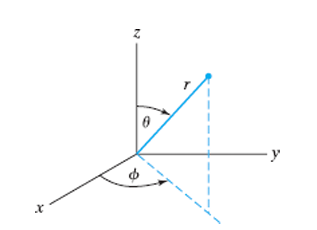
\includegraphics[width=0.4\textwidth]{Figures/5.5.png}
        \caption{球面坐标}
        \label{fig:5.5}
    \end{figure}

    现在,使用这些算符在空间直角坐标系中的形式,我们尝试求出$\hat{L}^2$和$\hat{L}_z$的本征函数和本征值。然而,我们会发现得到的偏微分方程无法分离变量。因此,我们将这些算符转换为\textbf{球面坐标}(spherical coordinate)。坐标$r$表示点$\left(x,y,z\right)$到原点的距离。而角度$\theta$是矢量$\mathbf{r}$与$z$轴正半轴之间的夹角,$\phi$是矢量$\mathbf{r}$在$xOy$平面上的投影与$x$轴正半轴之间的夹角(数学书通常将$\theta$与$\phi$互换)。使用三角法计算,有
    \begin{equation}
        x = r\sin\theta\cos\phi, \quad y = r\sin\theta\sin\phi, \quad z = r\cos\theta
        \label{eq:5.51}
    \end{equation}
    \begin{equation}
        r^2 = x^2 + y^2 + z^2, \quad \cos\theta = \frac{z}{\left(x^2+y^2+z^2\right)^{1/2}}, \quad \tan\phi = \frac{y}{x}
        \label{eq:5.52}
    \end{equation}

    为了将角动量算符转换为球坐标,我们需要对$\partial /\partial x$、$\partial /\partial y$和$\partial /\partial z$进行球坐标变换[如果需要,可以略读这一变换。在 (\ref{eq:5.64}) 之后重新开始阅读]。
    \begin{quote}
        \small 要进行这种变换,我们需要使用\textit{链式法则}(chain rule)。假设我们有一个关于$r$、$\theta$和$\phi$的函数$f\left(r,\theta,\phi\right)$。如果我们改变自变量,将
        \begin{equation*}
            r =r\left(x,y,z\right), \quad \theta = \theta\left(x,y,z\right), \quad \phi = \phi\left(x,y,z\right)
        \end{equation*}
        带入$f$,我们就将其变换为$x$、$y$和$z$的函数
        \begin{equation*}
            f\left[r\left(x,y,z\right),\theta\left(x,y,z\right),\phi\left(x,y,z\right)\right] = g\left(x,y,z\right)
        \end{equation*}
        例如,假设$f\left(r,\theta,\phi\right) = 3r\cos\theta+2\tan^2\phi$。使用式(\ref{eq:5.52}),我们有$g\left(x,y,z\right) = 3z+2y^{2}/x^{2}$。

        链式法则告诉我们$g\left(x,y,z\right)$的偏导数是如何与$f\left(r,\theta,\phi\right)$的偏导数联系起来的。事实上,
        \begin{equation}
            \left(\frac{\partial g}{\partial x}\right)_{y,z} = \left(\frac{\partial f}{\partial r}\right)_{\theta,\phi}\left(\frac{\partial r}{\partial x}\right)_{y,z} + \left(\frac{\partial f}{\partial \theta}\right)_{r,\phi}\left(\frac{\partial \theta}{\partial x}\right)_{y,z} + \left(\frac{\partial f}{\partial \phi}\right)_{r,\theta}\left(\frac{\partial \phi}{\partial x}\right)_{y,z}
            \label{eq:5.53}
        \end{equation}
        \begin{equation}
            \left(\frac{\partial g}{\partial y}\right)_{x,z} = \left(\frac{\partial f}{\partial r}\right)_{\theta,\phi}\left(\frac{\partial r}{\partial y}\right)_{x,z} + \left(\frac{\partial f}{\partial \theta}\right)_{r,\phi}\left(\frac{\partial \theta}{\partial y}\right)_{x,z} + \left(\frac{\partial f}{\partial \phi}\right)_{r,\theta}\left(\frac{\partial \phi}{\partial y}\right)_{x,z}
            \label{eq:5.54}
        \end{equation}
        \begin{equation}
            \left(\frac{\partial g}{\partial z}\right)_{x,y} = \left(\frac{\partial f}{\partial r}\right)_{\theta,\phi}\left(\frac{\partial r}{\partial z}\right)_{x,y} + \left(\frac{\partial f}{\partial \theta}\right)_{r,\phi}\left(\frac{\partial \theta}{\partial z}\right)_{x,y} + \left(\frac{\partial f}{\partial \phi}\right)_{r,\theta}\left(\frac{\partial \phi}{\partial z}\right)_{x,y}
            \label{eq:5.55}
        \end{equation}
        为了将这些方程转换为算符方程,我们删去$f$和$g$,得出
        \begin{equation}
            \frac{\partial}{\partial x} = \left(\frac{\partial r}{\partial x}\right)_{y,z}\frac{\partial}{\partial r} + \left(\frac{\partial \theta}{\partial x}\right)_{y,z}\frac{\partial}{\partial \theta} + \left(\frac{\partial \phi}{\partial x}\right)_{y,z}\frac{\partial}{\partial \phi}
            \label{eq:5.56}
        \end{equation}
        $\partial /\partial y$和$\partial /\partial z$的方程类似。现在的任务是计算类似于$\left(\partial r/\partial x\right)_{y,z}$的偏导数。将(\ref{eq:5.52})中第一个方程在$y$和$z$恒定的条件下对$x$求偏导数,我们有
        \begin{equation*}
            2r\left(\frac{\partial r}{\partial x}\right)_{y,z} = 2x = 2r\sin\theta\cos\phi
        \end{equation*}
        \begin{equation}
            \left(\frac{\partial r}{\partial x}\right)_{y,z} = \sin\theta\cos\phi
            \label{eq:5.57}
        \end{equation}
        将式$r^2 = x^2 + y^2 + z^2$对$y$和$z$求偏导数,我们有
        \begin{equation}
            \left(\frac{\partial r}{\partial y}\right)_{x,z} = \sin\theta\cos\phi, \quad \left(\frac{\partial r}{\partial z}\right)_{x,y} = \cos\theta
            \label{eq:5.58}
        \end{equation}
        由(\ref{eq:5.52})中第二个方程,我们有
        \begin{equation*}
            -\sin\theta\left(\frac{\partial \theta}{\partial x}\right)_{y,z} = -\frac{xz}{r^3}
        \end{equation*}
        \begin{equation}
            \left(\frac{\partial \theta}{\partial x}\right)_{y,z} = \frac{\cos\theta\cos\phi}{r}
            \label{eq:5.59}
        \end{equation}
        同样地,
        \begin{equation}
            \left(\frac{\partial \theta}{\partial y}\right)_{x,z} = \frac{\cos\theta\sin\phi}{r}, \quad \left(\frac{\partial \theta}{\partial z}\right)_{x,y} = -\frac{\sin\theta}{r}
            \label{eq:5.60}
        \end{equation}
        由$\tan\phi = y/x$,我们有
        \begin{equation}
            \left(\frac{\partial\phi}{\partial x}\right)_{y,z} = -\frac{\sin\phi}{r\sin\theta}, \quad \left(\frac{\partial\phi}{\partial y}\right)_{x,z} = \frac{\cos\phi}{r\sin\theta}, \quad \left(\frac{\partial\phi}{\partial z}\right)_{x,y} = 0
            \label{eq:5.61}
        \end{equation}
        将(\ref{eq:5.57})、(\ref{eq:5.59})和(\ref{eq:5.61})代入(\ref{eq:5.56}),我们得到
        \begin{equation}
            \frac{\partial}{\partial x} = \sin\theta\cos\phi\frac{\partial}{\partial r} + \frac{\cos\theta\cos\phi}{r}\frac{\partial}{\partial \theta} - \frac{\sin\phi}{r\sin\theta}\frac{\partial}{\partial \phi}
            \label{eq:5.62}
        \end{equation}
        类似地,我们可以得到
        \begin{equation}
            \frac{\partial}{\partial y} = \sin\theta\sin\phi\frac{\partial}{\partial r} + \frac{\cos\theta\sin\phi}{r}\frac{\partial}{\partial \theta} + \frac{\cos\phi}{r\sin\theta}\frac{\partial}{\partial \phi}
            \label{eq:5.63}
        \end{equation}
        \begin{equation}
            \frac{\partial}{\partial z} = \cos\theta\frac{\partial}{\partial r} - \frac{\sin\theta}{r}\frac{\partial}{\partial \theta}
            \label{eq:5.64}
        \end{equation}
    \end{quote}

    最后,我们可以用球面坐标来表示角动量分量了。将(\ref{eq:5.51})、(\ref{eq:5.63})和(\ref{eq:5.64})带入(\ref{eq:5.40}),得到
    \begin{equation*}
        \begin{aligned}
            \hat{L}_x & = -\mathrm{i}\hbar\left[r\sin\theta\sin\phi\left(\cos\theta\frac{\partial}{\partial r}\right) - \frac{\sin\theta}{r}\frac{\partial }{\partial\theta}\right.\\
            &  \quad \left.-r\cos\theta\left(\sin\theta\sin\phi\frac{\partial}{\partial r} +\frac{\cos\theta\sin\phi}{r}\frac{\partial}{\partial \phi}+\frac{\cos\phi}{r\sin\theta}\frac{\partial}{\partial \phi}\right)\right]
        \end{aligned}
    \end{equation*}
    \begin{equation}
        \hat{L}_x = \mathrm{i}\hbar\left(\sin\phi\frac{\partial}{\partial \theta} - \cos\theta\cos\phi\frac{\partial}{\partial \phi}\right)
        \label{eq:5.65}
    \end{equation}
    同样,我们有
    \begin{equation}
        \hat{L}_y = -\mathrm{i}\hbar\left(\cos\phi\frac{\partial}{\partial \theta} - \cot\theta\sin\phi\frac{\partial}{\partial \phi}\right)
        \label{eq:5.66}
    \end{equation}
    \begin{equation}
        \hat{L}_z = -\mathrm{i}\hbar\frac{\partial}{\partial \phi}
        \label{eq:5.67}
    \end{equation}

    对$\hat{L}_x$、$\hat{L}_y$和$\hat{L}_z$进行平方并相加,我们可以构造出$\hat{L}^2 = \hat{L}_x^2 + \hat{L}_y^2 + \hat{L}_z^2$[式(\ref{eq:5.43})]。结果为(问题5.17)
    \begin{equation}
        \hat{L}^2 = -\hbar^2\left(\frac{\partial^2}{\partial\theta^2} + \cot\theta\frac{\partial}{\partial\theta} + \frac{1}{\sin^2\theta}\frac{\partial^2}{\partial \phi^2}\right)
        \label{eq:5.68}
    \end{equation}

    虽然角动量算符取决于所有三个直角坐标$x$、$y$和$z$,但它们只涉及两个球面坐标$\theta$和$\phi$。

\subsection*{单粒子轨道角动量的本征函数和本征值}
    我们现在希望找到$\hat{L}^2$和$\hat{L}_z$的共同本征函数,记作$Y$。由于这些算符只涉及$\theta$和$\phi$,那么$Y$就是这两个变量的函数:$Y = Y\left(\theta,\phi\right)$(当然,由于这些算符都是线性算符,我们可以用任意一个关于$r$的函数乘以$Y$而不改变$Y$是$\hat{L}^2$和$\hat{L}_z$的本征函数的事实)。我们必须解以下方程:
    \begin{equation}
        \hat{L}_zY\left(\theta,\phi\right) = bY\left(\theta,\phi\right)
        \label{eq:5.69}
    \end{equation}
    \begin{equation}
        \hat{L}^2Y\left(\theta,\phi\right) = cY\left(\theta,\phi\right)
        \label{eq:5.70}
    \end{equation}
    其中$b$和$c$分别是$\hat{L}_z$和$\hat{L}^2$的本征值。

    使用算符$\hat{L}_z$,我们有
    \begin{equation}
        -\mathrm{i}\hbar\frac{\partial}{\partial \phi}Y\left(\theta,\phi\right) = bY\left(\theta,\phi\right)
        \label{eq:5.71}
    \end{equation}
    由于(\ref{eq:5.71})中的算符不涉及$\theta$,我们可以尝试分离变量。将$Y$写成
    \begin{equation}
        Y\left(\theta,\phi\right) = S\left(\theta\right)T\left(\phi\right)
        \label{eq:5.72}
    \end{equation}
    则方程(\ref{eq:5.71})变为
    \begin{equation*}
        -\mathrm{i}\hbar\frac{\partial}{\partial \phi}\left[S\left(\theta\right)T\left(\phi\right)\right] = bS\left(\theta\right)T\left(\phi\right)
    \end{equation*}
    \begin{equation*}
        -\mathrm{i}\hbar S\left(\theta\right)\frac{\mathrm{d}T\left(\phi\right)}{\mathrm{d}\phi} = bS\left(\theta\right)T\left(\phi\right)
    \end{equation*}
    \begin{equation*}
        \frac{\mathrm{d}T\left(\phi\right)}{T\left(\phi\right)} = \frac{\mathrm{i}b}{\hbar}\mathrm{d}\phi
    \end{equation*}
    \begin{equation}
        T\left(\phi\right) = A e^{\mathrm{i}b\phi/\hbar}
        \label{eq:5.73}
    \end{equation}
    其中$A$是任意常数。

    $T$适合作为本征函数吗。答案是否定的,因为它一般不是单值函数。如果我们将$\phi$增加$2\pi$,我们仍将处于空间中的同一点,因此我们希望这样做时 $T$ 保持不变。为了使$T$成为单值函数,我们需要做如下限制:
    \begin{equation*}
        T\left(\phi + 2\pi\right) = T\left(\phi\right)
    \end{equation*}
    \begin{equation*}
        A e^{\mathrm{i}b\phi/\hbar}\mathrm{e}^{\mathrm{i}b2\pi/\hbar} = A e^{\mathrm{i}b\phi/\hbar}
    \end{equation*}
    \begin{equation}
        \mathrm{e}^{\mathrm{i}b2\pi/\hbar} = 1
        \label{eq:5.74}
    \end{equation}

    为了满足$\mathrm{e}^{\mathrm{i}\alpha} = \cos\alpha + \mathrm{i}\sin\alpha = 1$,我们需要$\alpha = 2\pi m$,其中
    \begin{equation*}
        m = 0, \pm 1, \pm 2, \pm\ldots
    \end{equation*}
    因此,由式(\ref{eq:5.74})我们得到
    \begin{equation*}
        2\pi b/\hbar = 2\pi m
    \end{equation*}
    \begin{equation}
        b = m\hbar, \quad m = \ldots, -2, -1, 0, 1, 2, \ldots
        \label{eq:5.75}
    \end{equation}
    式(\ref{eq:5.73})变为
    \begin{equation}
        T\left(\phi\right) = A e^{\mathrm{i}m\phi}, \quad m = 0, \pm 1, \pm 2, \ldots
        \label{eq:5.76}
    \end{equation}
    角动量在$z$方向分量的本征值是量子化的。

    通过归一化$T$,我们可以确定常数$A$。首先,让我们考虑对关于$r$、$\theta$和$\phi$的函数$F$进行归一化。三个独立变量的取值范围是(见图\ref{fig:5.5})
    \begin{equation}
        \boxed{
            0 \le r \le \infty, \quad 0 \le \theta \le \pi, \quad 0 \le \phi < 2\pi
        }
        \label{eq:5.77}
    \end{equation}
    球坐标系下的体积微元为(\textit{Taylor and Mann},第13.9节)
    \begin{equation}
        \boxed{
            \mathrm{d}\tau = r^2\sin\theta \: \mathrm{d}r \: \mathrm{d}\theta \: \mathrm{d}\phi
        }
        \label{eq:5.78}
    \end{equation}
    (\ref{eq:5.78})是一个无限小区域空间的体积,其球面坐标位于$r$到$r+\mathrm{d}r$、$\theta$到$\theta+\mathrm{d}\theta$和$\phi$到$\phi+\mathrm{d}\phi$之间。因此,球坐标下$F$的归一化条件为
    \begin{equation}
        \int_{0}^{\infty}\left[\int_{0}^{\pi}\left[\int_{0}^{2\pi}\left|F\left(r,\theta,\phi\right)\right|^2 \mathrm{d}\phi\right]\sin\theta \mathrm{d}\theta\right]r^2\mathrm{d}r = 1
        \label{eq:5.79}
    \end{equation}
    如果$F$恰好可以写成
    \begin{equation*}
        F\left(r,\theta,\phi\right) = R\left(r\right)S\left(\theta\right)T\left(\phi\right)
    \end{equation*}
    则对(\ref{eq:5.79})使用积分(\ref{eq:3.74}),有
    \begin{equation*}
        \int_{0}^{\infty}\left|R\left(r\right)\right|^2 r^2 \mathrm{d}r \int_{0}^{\pi}\left|S\left(\theta\right)\right|^2 \sin\theta \: \mathrm{d}\theta \int_{0}^{2\pi}\left|T\left(\phi\right)\right|^2 \mathrm{d}\phi = 1
    \end{equation*}
    方便的做法是将$F$的每个因子都作归一化处理:
    \begin{equation}
        \int_{0}^{\infty}\left|R\left(r\right)\right|^2 r^2 \mathrm{d}r = 1, \quad \int_{0}^{\pi}\left|S\left(\theta\right)\right|^2 \sin\theta \: \mathrm{d}\theta = 1, \quad \int_{0}^{2\pi}\left|T\left(\phi\right)\right|^2 \mathrm{d}\phi = 1
        \label{eq:5.80}
    \end{equation}
    因此,
    \begin{equation*}
        \int_{0}^{2\pi}\left(A\mathrm{e}^{\mathrm{i}m\phi}\right)^{\ast}\left(A\mathrm{e}^{\mathrm{i}m\phi}\right) \mathrm{d}\phi = 1 = \left|A\right|^2\int_{0}^{2\pi} \mathrm{d}\phi
    \end{equation*}
    \begin{equation*}
        \left|A\right| = \left(2\pi\right)^{-1/2}
    \end{equation*}
    \begin{equation}
        T\left(\phi\right) = \frac{1}{\sqrt{2\pi}}e^{\mathrm{i}m\phi}, \quad m = 0, \pm 1, \pm 2, \ldots
        \label{eq:5.81}
    \end{equation}

    我们现在尝试使用式(\ref{eq:5.70})来求解$\hat{L}^2$的本征值$c$。对$\hat{L}^2$使用式(\ref{eq:5.68})、对$Y$使用式(\ref{eq:5.72}),由式(\ref{eq:5.81}),我们有
    \begin{equation*}
        -\hbar^2\left(\frac{\partial^2}{\partial\theta^2} + \cot\theta\frac{\partial}{\partial\theta} + \frac{1}{\sin^2\theta}\frac{\partial^2}{\partial\phi^2}\right)\left(S\left(\theta\right)\frac{1}{\sqrt{2\pi}}e^{\mathrm{i}m\phi}\right) = cS\left(\theta\right)\frac{1}{\sqrt{2\pi}}e^{\mathrm{i}m\phi}
    \end{equation*}
    \begin{equation}
        \frac{\mathrm{d}^2S}{\mathrm{d}\theta^2}+\cot\theta\frac{\mathrm{d}S}{\mathrm{d}\theta} - \frac{m^2}{\sin^2\theta}S = -\frac{c}{\hbar^2}S
        \label{eq:5.82}
    \end{equation}
    \begin{quote}
        \small
        \noindent 为了解方程(\ref{eq:5.82}),我们需要进行一些繁琐的操作,如果需要,可以略过不读。在式(\ref{eq:5.91})处重新开始阅读。首先,为了方便起见,我们将自变量代替为
        \begin{equation}
            w = \cos\theta
            \label{eq:5.83}
        \end{equation}
        将$S$变换为一个新的关于$w$的函数:
        \begin{equation}
            S\left(\theta\right) = G\left(w\right)
            \label{eq:5.84}
        \end{equation}
        由链式法则,我们有
        \begin{equation}
            \frac{\mathrm{d}S}{\mathrm{d}\theta} = \frac{\mathrm{d}G}{\mathrm{d}w}\frac{\mathrm{d}w}{\mathrm{d}\theta} = -\sin\theta\frac{\mathrm{d}G}{\mathrm{d}w} = -\left(1-w^2\right)^{1/2}\frac{\mathrm{d}G}{\mathrm{d}w}
            \label{eq:5.85}
        \end{equation}
        同样地,我们得出(问题5.25)
        \begin{equation}
            \frac{\mathrm{d}^2S}{\mathrm{d}\theta^2} = \left(1-w^2\right)\frac{\mathrm{d}^2G}{\mathrm{d}w^2} - w\frac{\mathrm{d}G}{\mathrm{d}w}
            \label{eq:5.86}
        \end{equation}
        由式(\ref{eq:5.86})、(\ref{eq:5.85})和$\cot\theta = \cos\theta/\sin\theta = w/\left(1-w^2\right)^{1/2}$,我们可以将(\ref{eq:5.82})重写为
        \begin{equation}
            \left(1-w^2\right)\frac{\mathrm{d}^2G}{\mathrm{d}w^2} - 2w\frac{\mathrm{d}G}{\mathrm{d}w}+\left[\frac{c}{\hbar^2}-\frac{m^2}{1-w^2}\right]G\left(w\right) = 0
            \label{eq:5.87}
        \end{equation}
        $w$的取值范围是$-1 \le w \le 1$。

        在尝试幂级数求解时,为了得到两项的递推关系,我们需要对因变量作如下改变:
        \begin{equation}
            G\left(w\right) = \left(1-w^2\right)^{\left|m\right|/2}H\left(w\right)
            \label{eq:5.88}
        \end{equation}
        对(\ref{eq:5.88})求导,我们得到了$G^{\prime}$和$G^{\prime\prime}$,在除以$\left(1-w^2\right)^{\left|m\right|/2}$后,我们可以将(\ref{eq:5.87})变为
        \begin{equation}
            \left(1-w^2\right)H^{\prime\prime} - 2\left(\left|m\right|+1\right)wH^{\prime} + \left[c\hbar^{-2}-\left|m\right|\left(\left|m\right|+1\right)\right]H = 0
            \label{eq:5.89}
        \end{equation}
        现在,我们尝试$H$的幂级数解
        \begin{equation}
            H\left(w\right) = \sum_{n=0}^{\infty}a_jw^j
            \label{eq:5.90}
        \end{equation}
        对其求导[与式(\ref{eq:4.36})-(\ref{eq:4.38})类似],我们有
        \begin{equation*}
            H^{\prime}\left(w\right) = \sum_{j=0}^{\infty}ja_jw^{j-1}
        \end{equation*}
        \begin{equation*}
            H^{\prime\prime}\left(w\right) = \sum_{j=0}^{\infty}j(j-1)a_jw^{j-2} = \sum_{j=0}^{\infty}\left(j+2\right)\left(j+1\right)a_{j+2}w^{j}
        \end{equation*}
        将这些幂级数带入式(\ref{eq:5.89}),合并求和后,有
        \begin{equation*}
            \sum_{j=0}^{\infty}\left[\left(j+2\right)\left(j+1\right)a_{j+2}+\left(-j^2-j-2\left|m\right|j+\frac{c}{\hbar^2}-\left|m\right|^2-\left|m\right|\right)a_j\right]w^j=0
        \end{equation*}
        令$w^j$的系数为零,我们得到
        \begin{equation}
            a_{j+2} = \frac{\left(j+\left|m\right|\right)\left(j+\left|m\right|+1\right)-c/\hbar^{-2}}{\left(j+1\right)\left(j+2\right)}a_j
            \label{eq:5.91}
        \end{equation}
    \end{quote}

    与谐振子的例子一样,式(\ref{eq:5.89})的通解也是偶次幂级数(系数由$a_0$决定)和奇次幂级数(系数由$a_1$决定)的任意线性组合。可以证明,由式(\ref{eq:5.91})定义的无穷级数不是品优函数。[许多文献都指出:该级数在$w = \pm 1$处发散。然而,这并不足以否定该无穷级数,因为本征函数是平方可积的,即使在某两点上是无穷的。仔细讨论见 M. Whippman, Am. Phys., 34, 656 (1966)。]因此,与谐振子的情况一致,我们必须让级数在某一项$a_kw^k$处打断。根据$k$是奇数还是偶数,我们设$a_0$或$a_1$为零,从而消除其他级数。

    令式(\ref{eq:5.91})中$a_k$的系数为零,得到
    \begin{equation}
        c = \hbar^2\left(k+\left|m\right|\right)\left(k+\left|m\right|+1\right), \quad k = 0, 1, 2, \ldots
        \label{eq:5.92}
    \end{equation}
    由于$\left|m\right|$的值为$0, 1, 2, \ldots$,$k+\left|m\right|$的值为$0, 1, 2, \ldots$。因此,我们可以定义量子数$l$为
    \begin{equation}
        l = k + \left|m\right|
        \label{eq:5.93}
    \end{equation}
    角动量大小平方的本征值为
    \begin{equation}
        c = l\left(l+1\right)\hbar^2, \quad l = 0, 1, 2, \ldots
        \label{eq:5.94}
    \end{equation}
    单粒子轨道角动量的大小为
    \begin{equation}
        \left|\mathbf{L}\right| = \left[l\left(l+1\right)\right]^{1/2}\hbar
        \label{eq:5.95}
    \end{equation}

    由式(\ref{eq:5.93})有$\left|m\right| = l$。因此,$m$的取值范围为
    \begin{equation}
        m = -l, -l+1, -l+2, \ldots, -1, 0, 1, \ldots, l-2, l-1, l, l
        \label{eq:5.96}
    \end{equation}

    现在让我们检查角动量的本征函数。由式(\ref{eq:5.83})、(\ref{eq:5.84})、(\ref{eq:5.88})、(\ref{eq:5.90})和(\ref{eq:5.93}),本征函数中的$\theta$因子为
    \begin{equation}
        S_{l,m}\left(\theta\right) = \sin^{\left|m\right|}\theta\sum_{\substack{j=1,3,\ldots \\ j=0,2,\ldots}}^{l-\left|m\right|}a_j\cos^j\theta
        \label{eq:5.97}
    \end{equation}
    其中,$l-\left|m\right|$的奇偶性决定求和从$j=1$还是$j=0$开始。使用式(\ref{eq:5.94}),$a_j$的系数满足的递推关系(\ref{eq:5.91})可以写成
    \begin{equation}
        a_{j+2} = \frac{\left(j+\left|m\right|\right)\left(j+\left|m\right|+1\right)-l\left(l+1\right)}{\left(j+1\right)\left(j+2\right)}a_j
        \label{eq:5.98}
    \end{equation}

    $\hat{L}^2$和$\hat{L}_z$的本征函数由式(\ref{eq:5.72})和式(\ref{eq:5.81})给出:
    \begin{equation}
        \boxed{
            Y^m_l\left(\theta,\phi\right) = S_{l,m}\left(\theta\right)T\left(\phi\right) = \frac{1}{\sqrt{2\pi}}S_{l,m}\left(\theta\right)e^{\mathrm{i}m\phi}
        }
        \label{eq:5.99}
    \end{equation}
    $Y^m_l$中的$m$是一个标签,而不是指数。
    \begin{examplebox}
        \textbf{例题:}分别求当(a)$l=0$;(b)$l=1$时$Y_l^m\left(\theta,\phi\right)$、$\hat{L}^2$和$\hat{L}_z$的本征值。
        \\

        \textbf{(a)}对于$l=0$,由式(\ref{eq:5.96}),有$m=0$。则式(\ref{eq:5.97})变为
        \begin{equation}
            S_{0,0}\left(\theta\right) = a_0
            \label{eq:5.100}
        \end{equation}
        由归一化条件(\ref{eq:5.80}),我们有
        \begin{equation*}
            \int_{0}^{\pi}\left|a_0\right|^2 \sin\theta \: \mathrm{d}\theta = 1 = 2\left|a_0\right|^2
        \end{equation*}
        \begin{equation*}
            \left|a_0\right| = 2^{-1/2}
        \end{equation*}
        则式(\ref{eq:5.99})变为
        \begin{equation}
            Y^0_0\left(\theta,\phi\right) = \frac{1}{\sqrt{4\pi}}
            \label{eq:5.101}
        \end{equation}
        [显然,式(\ref{eq:5.101})是$\hat{L}^2$、$\hat{L}_x$、$\hat{L}_y$和$\hat{L}_z$的本征函数,方程(\ref{eq:5.65})-(\ref{eq:5.68})。]对于$l=0$,本征函数不存在角度依赖关系,我们说本征函数是\textbf{球对称的}(spherically symmetric)。

        对于$l=0$和$m=0$,由式(\ref{eq:5.69})、(\ref{eq:5.70})、(\ref{eq:5.75})和(\ref{eq:5.94}),我们有$\hat{L}^2$的本征值为$c=0$,$\hat{L}_z$的本征值为$b=0$。

        \textbf{(b)} 对于$l=1$,由式(\ref{eq:5.96}),有$m=-1, 0, 1$。当$\left|m\right| = 1$时,式(\ref{eq:5.97})变为
        \begin{equation}
            S_{1,\pm 1}\left(\theta\right) = a_0\sin\theta
            \label{eq:5.102}
        \end{equation}
        (\ref{eq:5.102})中的$a_0$和(\ref{eq:5.100})中的$a_0$不一定相等。由归一化条件,有
        \begin{equation*}
            1 = \left|a_0^2\right|\int_{0}^{\pi}\sin^2\theta\sin\theta \: \mathrm{d}\theta = \left|a_0^2\right|\int_{-1}^{1}\left(1-w^2\right) \: \mathrm{d}w
        \end{equation*}
        \begin{equation*}
            \left|a_0\right| = \sqrt{3}/2
        \end{equation*}
        其中,我们将$w$用$\cos\theta$代替。因此,我们有$S_{1,\pm 1}\left(3^{1/2}/2\right)\sin\theta$,式(\ref{eq:5.99})变为
        \begin{equation}
            Y_1^1 = \left(3/8\pi\right)^{1/2}\sin\theta e^{\mathrm{i}\phi}, \quad Y_1^{-1} = \left(3/8\pi\right)^{1/2}\sin\theta e^{-\mathrm{i}\phi}
            \label{eq:5.103}
        \end{equation}
        当$l=1$而$m=0$时,我们得出(见下文的练习题)$S_{1,0} = \left(3/2\right)^{1/2}\cos\theta$,$Y_1^0 = \left(3/4\pi\right)^{1/2}\cos\theta$。因此,当$l=1$时,由式(\ref{eq:5.94})可得$\hat{L}^2$的本征值为$2\hbar^2$;由式(\ref{eq:5.75}),$\hat{L}_z$的本征值为$\hbar$、$0$和$-\hbar$,分别与$m=1, 0, -1$对应。
        \\

        \textbf{练习:}验证$S_{1,0}$和$Y_1^0$的表达式。
    \end{examplebox}

    函数$S_{l,m}\left(\theta\right)$在数学中是众所周知的,是乘以一个归一化系数后的\textit{连带勒让德函数}(associated Legendre function)。连带勒让德函数的定义见问题5.34。表(\ref{tab:5.1})列出了$l \le 3$的$S_{l,m}\left(\theta\right)$表达式。
    \begin{table}[htbp]
        \centering
        \caption{$S_{l,m}\left(\theta\right)$}
        \label{tab:5.1}
        \begin{tabular}{|l|l|}
            \hline
            $l=0$: & $S_{0,0} = \frac{1}{2}\sqrt{2}$ \\
            \hline
            $l=1$: & $S_{1,0} = \frac{1}{2}\sqrt{6}\cos\theta$ \\
            & $S_{1,\pm 1} = \frac{1}{2}\sqrt{3}\sin\theta$ \\
            \hline
            $l=2$: & $S_{2,0} = \frac{1}{4}\sqrt{10}\left(3\cos^2\theta - 1\right)$ \\
            & $S_{2,\pm 1} = \frac{1}{2}\sqrt{15}\sin\theta\cos\theta$ \\
            & $S_{2,\pm 2} = \frac{1}{4}\sqrt{15}\sin^2\theta$ \\
            \hline
            $l=3$: & $S_{3,0} = \frac{3}{4}\sqrt{14}\left(\frac{5}{3}\cos^3\theta-\cos\theta\right)$ \\
            & $S_{3, \pm 1} = \frac{1}{8}\sqrt{42}\sin\theta\left(5\cos^2\theta - 1\right)$ \\
            & $S_{3, \pm 2} = \frac{1}{4}\sqrt{105}\sin^2\theta\cos\theta$ \\
            & $S_{3, \pm 3} = \frac{1}{8}\sqrt{70}\sin^3\theta$ \\
            \hline
        \end{tabular}
    \end{table}
    \begin{equation}
        \boxed{
            \hat{L}^2Y^m_l\left(\theta,\phi\right) = l\left(l+1\right)\hbar^2Y^m_l\left(\theta,\phi\right), \quad l = 0, 1, 2, \ldots
        }
        \label{eq:5.104}
    \end{equation}
    \begin{equation}
        \boxed{
            \hat{L}_zY^m_l\left(\theta,\phi\right) = m\hbar Y^m_l\left(\theta,\phi\right), \quad m = -l, -l+1, \ldots, l-1, l
        }
        \label{eq:5.105}
    \end{equation}
    其中,本征函数由式(\ref{eq:5.99})给出。我们通常使用符号$m_l$代替$m$来表示$L_z$量子数。我们稍后会看到球谐函数是正交函数(方程7.27)。

    由于$l \ge \left|m\right|$,因此除了$l=0$以外,轨道角动量$\mathbf{L}$的大小$\left[l\left(l+1\right)\right]^{1/2}\hbar^2$大于其$z$方向的分量$\left|m\right|\hbar$。如果可以让角动量的大小等于其 $z$ 分量,这就意味着 $x$ 和 $y$ 分量为零,我们就可以指定 $\mathbf{L}$ 的所有三个分量了。然而这是做不到的,因为角动量三个分量的算符不可对易。只有一种例外,就是$l$为零时。在该情况中,$\left|\mathbf{L}\right|^2 = L_x^2+ L_y^2 + L_z^2 = 0$,因此所有三个分量都为零。由式(\ref{eq:5.12}),角动量分量的不确定性满足
    \begin{equation}
        \Delta L_x\Delta L_y \ge \left|\frac{1}{2}\Psi^{\ast}\left[\hat{L}_x,\hat{L}_y\right]\Psi\mathrm{d}\tau\right| = \frac{\hbar}{2}\left|\int \Psi^{\ast}\hat{L}_z\Psi\mathrm{d}\tau\right|
        \label{eq:5.106}
    \end{equation}
    通过循环排列能得出其余两个相似的方程。当$\hat{L}_x$、$\hat{L}_y$和$\hat{L}_z$的本征值为零时,$\hat{L}_x\Psi = 0$,$\hat{L}_y\Psi = 0$,$\hat{L}_z\Psi = 0$,式(\ref{eq:5.106})的右侧和另两个相似的方程也为零,因此$\Delta L_x = \Delta L_y = \Delta L_z = 0$被允许。然而,根据第\ref{sec:5.1 Simultaneous Specification of Several Properties}节,要同时得到两个算符的本征函数,这两个算符必须可对易,这又是怎么回事呢?答案是,这个定理指的是一个算符的整套本征函数是另一个算符的本征函数的可能性。因此,尽管$\hat{L}_x$和$\hat{L}_z$不可对易,但仍有可能使得$\hat{L}_x$的本征函数同时也是$\hat{L}_z$的本征函数($l=0=m$时)。然而,使得$\hat{L}_x$的\textit{所有}本征函数都是$\hat{L}_z$的本征函数是不可能的。
    \begin{figure}[h!]
        \centering
        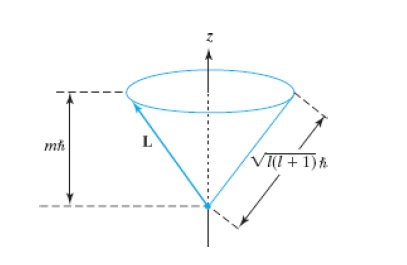
\includegraphics[width=0.5\textwidth]{Figures/5.6.png}
        \caption{$\mathbf{L}$的方向}
        \label{fig:5.6}
    \end{figure}
    \begin{figure}
        \centering
        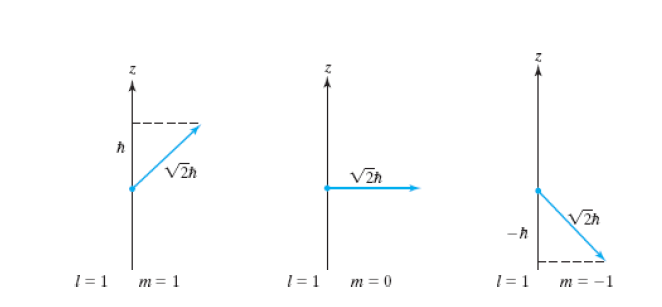
\includegraphics[width=0.5\textwidth]{Figures/5.7.png}
        \caption{$l=1$时$\mathbf{L}$相对于$z$轴的方向}
        \label{fig:5.7}
    \end{figure}

    由于我们无法指定$L_x$和$L_y$,所以矢量$\mathbf{L}$可以位于以$z$轴为轴,高度为$m\hbar$的圆锥面上的任何位置。当$l=1$时,$\mathbf{L}$相对于$z$轴的可能方向如图\ref{fig:5.7}所示。对于每一个$\hat{L}^2$的本征值,都有$2l+1$个不同的本征函数$Y_l^m$,与$m$的$2l+1$个取值相对应。我们说$\hat{L}^2$的本征值是$\left(2l+1\right)$重简并的,\textbf{简并}(degeneracy)一词适用于任何算符的本征值,而不仅仅是哈密顿算符。

    当然,$z$轴并没有什么特别之处。空间中的所有方向都是等价的。如果我们选择确定$L^2$和$L_x$(而不是$L_z$),我们会得到与$L_z$相同的$L_x$的本征值。然而,解$\hat{L}_z$的本征方程更为简单,因为在球坐标系中,$\hat{L}_z$的形式更简单,其中涉及到围绕$z$轴的旋转角度$\phi$。

\section{角动量阶梯算符法}
\label{sec:5.4 The Ladder-Operator Method for Angular Momentum}
    通过将轨道角动量的算符表示为微分算符,并求解由此产生的微分方程,我们得到了$\hat{L}^2$和$\hat{L}_z$的本征值。我们现在证明:只需要利用算符之间的对易关系就能找到这些本征值。本节的工作适用于任何满足角动量对易关系的算符。它尤其适用于自旋角动量(第 \ref{chap:10} 章)和轨道角动量。

    我们使用字母$L$来表示轨道角动量。在这里,我们将使用字母 $M$ 来表示我们正在处理的任何一种角动量。我们有三个线性算符$\hat{M}_x$、$\hat{M}_y$和$\hat{M}_z$,我们只知道它们符合对易关系[与式(\ref{eq:5.46})和(\ref{eq:5.48})相似]
    \begin{equation}
        \left[\hat{M}_x,\hat{M}_y\right] = \mathrm{i}\hbar\hat{M}_z, \quad \left[\hat{M}_y,\hat{M}_z\right] = \mathrm{i}\hbar\hat{M}_x, \quad \left[\hat{M}_z,\hat{M}_x\right] = \mathrm{i}\hbar\hat{M}_y
        \label{eq:5.107}
    \end{equation}
    我们定义算符$\hat{M}^2$为
    \begin{equation}
        \hat{M}^2 = \hat{M}_x^2 + \hat{M}_y^2 + \hat{M}_z^2
        \label{eq:5.108}
    \end{equation}
    我们的问题是如何找到$\hat{M}^2$和$\hat{M}_z$的本征值。

    使用式(\ref{eq:5.107})和(\ref{eq:5.108}),我们从对$\hat{M}^2$及其分量的对易子进行评估开始。与推导(\ref{eq:5.49})和(\ref{eq:5.50})时的推导类似,我们有
    \begin{equation}
        \left[\hat{M}^2,\hat{M}_x\right] = \left[\hat{M}^2,\hat{M}_y\right] = \left[\hat{M}^2,\hat{M}_z\right] = 0
        \label{eq:5.109}
    \end{equation}
    因此,我们可以得到$\hat{M}^2$和$\hat{M}_z$的同时本征函数。

    现在我们定义两个新算符,\textbf{升算符}(raising operator)$\hat{M}_+$和\textbf{降算符}(lowering operator)$\hat{M}_-$,它们的定义为
    \begin{equation}
        \hat{M}_+ \equiv \hat{M}_x + \mathrm{i}\hat{M}_y
        \label{eq:5.110}
    \end{equation}
    \begin{equation}
        \hat{M}_- \equiv \hat{M}_x - \mathrm{i}\hat{M}_y
        \label{eq:5.111}
    \end{equation}
    这些是\textbf{阶梯算符}(ladder operator)的例子。使用这些术语的原因很快就会清楚。我们有
    \begin{equation*}
        \begin{aligned}
            \hat{M}_+\hat{M}_- & = \left(\hat{M}_x+\mathrm{i}\hat{M}_y\right)\left(\hat{M}_x-\mathrm{i}\hat{M}_y\right) = \hat{M}_x\left(\hat{M}_x-\mathrm{i}\hat{M}_y\right) + \mathrm{i}\hat{M}_y\left(\hat{M}_x-\mathrm{i}\hat{M}_y\right) \\
            & = \hat{M}_x^2 - \mathrm{i}\hat{M}_x\hat{M}_y + \mathrm{i}\hat{M}_y\hat{M}_x + \hat{M}_y^2 = \hat{M}^2 - \hat{M}_z^2 + \mathrm{i}\left[\hat{M}_y,\hat{M}_x\right]
        \end{aligned}
    \end{equation*}
    \begin{equation}
        \hat{M}_+\hat{M}_- = \hat{M}^2 - \hat{M}_z^2 + \hbar\hat{M}_z
        \label{eq:5.112}
    \end{equation}
    同样地,我们有
    \begin{equation}
        \hat{M}_-\hat{M}_+ = \hat{M}^2 - \hat{M}_z^2 - \hbar\hat{M}_z
        \label{eq:5.113}
    \end{equation}
    对于这些算符与$\hat{M}_z$的对易子,我们有
    \begin{equation*}
        \left[\hat{M}_+,\hat{M}_z\right] = \left[\hat{M}_x+\mathrm{i}\hat{M}_y,\hat{M}_z\right] = \left[\hat{M}_x,\hat{M}_z\right]+\mathrm{i}\left[\hat{M}_y,\hat{M}_z\right] = -\mathrm{i}\hbar\hat{M}_y - \hbar\hat{M}_x
    \end{equation*}
    \begin{equation*}
        \left[\hat{M}_+,\hat{M}_z\right] = -\hbar\hat{M}_+
    \end{equation*}
    \begin{equation}
        \hat{M}_+\hat{M}_z = \hat{M}_z\hat{M}_+ - \hbar\hat{M}_+
        \label{eq:5.114}
    \end{equation}
    其中我们用到了式(\ref{eq:5.107})。同样地,我们有
    \begin{equation}
        \hat{M}_-\hat{M}_z = \hat{M}_z\hat{M}_- + \hbar\hat{M}_-
        \label{eq:5.115}
    \end{equation}

    设$Y$是$\hat{M}^2$和$\hat{M}_z$的共同本征函数,即
    \begin{equation}
        \hat{M}^2Y = cY
        \label{eq:5.116}
    \end{equation}
    \begin{equation}
        \hat{M}_zY = bY
        \label{eq:5.117}
    \end{equation}
    其中$c$和$b$是本征值。将算符$\hat{M}_+$作用于式(\ref{eq:5.117}),我们有
    \begin{equation*}
        \hat{M}_+\hat{M}_zY = \hat{M}_+bY
    \end{equation*}
    使用式(\ref{eq:5.114}),及$\hat{M}_+$是线性算符,我们有
    \begin{equation*}
        \left(\hat{M}_z\hat{M}_+-\hbar\hat{M}_+\right)Y = b\hat{M}_+Y
    \end{equation*}
    \begin{equation}
        \hat{M}_z\left(\hat{M}_+Y\right) = \left(b+\hbar\right)\left(\hat{M}_+Y\right)
        \label{eq:5.118}
    \end{equation}
    最后一个方程说明:$\hat{M}_+Y$是算符$\hat{M}_z$的本征函数,其本征值为$b+\hbar$。换句话说,将升算符$\hat{M}_+$作用到本征函数$Y$上后,可以将$Y$转换成另一个$\hat{M}_z$的本征函数,其本征值比$Y$的大$\hbar$。如果我们现在对式(\ref{eq:5.118})使用升算符,并再次使用式(\ref{eq:5.114}),我们得到
    \begin{equation*}
        \hat{M}_z\left(\hat{M}_+^2Y\right) = \left(b+2\hbar\right)\left(\hat{M}_+^2Y\right)
    \end{equation*}
    重复应用升算符,有
    \begin{equation}
        \hat{M}_z\left(\hat{M}_+^kY\right) = \left(b+k\hbar\right)\left(\hat{M}_+^kY\right), \quad k = 0, 1, 2, \ldots
        \label{eq:5.119}
    \end{equation}

    如果我们对式(\ref{eq:5.117})使用降算符$\hat{M}_-$并应用式(\ref{eq:5.115}),我们已同样的方式发现:
    \begin{equation}
        \hat{M}_z\left(\hat{M}_-Y\right) = \left(b-\hbar\right)\left(\hat{M}_-Y\right)
        \label{eq:5.120}
    \end{equation}
    \begin{equation}
        \hat{M}_z\left(\hat{M}_-^kY\right) = \left(b-k\hbar\right)\left(\hat{M}_-^kY\right)
        \label{eq:5.121}
    \end{equation}

    这样,通过对本征值为$b$的本征函数使用升降算符,我们得到了一个本征值阶梯,阶梯之间的差值为$\hbar$:
    \begin{equation*}
        \ldots, \quad b-2\hbar, \quad b-\hbar, \quad b, \quad b+\hbar, \quad b+2\hbar, \quad \ldots
    \end{equation*}
    函数$\hat{M}_{\pm}^kY$是$\hat{M}_z$的本征函数,其本征值为$b \pm k\hbar$[式(\ref{eq:5.119})和(\ref{eq:5.121})]。我们现在表明这些函数也是$\hat{M}^2$的本征函数,其本征值为$c$:
    \begin{equation}
        \hat{M}_z\hat{M}_{\pm}^kY = \left(b \pm k\hbar\right)\hat{M}_{\pm}^kY
        \label{eq:5.122}
    \end{equation}
    \begin{equation}
        \hat{M}^2\hat{M}_{\pm}^kY = c\hat{M}_{\pm}^kY
        \label{eq:5.123}
    \end{equation}
    为了证明(\ref{eq:5.123}),我们首先表明$\hat{M}^2$与$\hat{M}_+$和$\hat{M}_-$对易。我们有
    \begin{equation*}
        \left[\hat{M}^2,\hat{M}_{\pm}\right] = \left[\hat{M}^2,\hat{M}_x\pm\mathrm{i}\hat{M}_y\right] = \left[\hat{M}^2,\hat{M}_x\right] \pm \mathrm{i}\left[\hat{M}^2,\hat{M}_y\right] = 0 \pm 0 = 0
    \end{equation*}
    也有
    \begin{equation*}
        \left[\hat{M}^2,\hat{M}_{\pm}^2\right] = \left[\hat{M}^2,\hat{M}_{\pm}\right]\hat{M}_{\pm} + \hat{M}_{\pm}\left[\hat{M}^2,\hat{M}_{\pm}\right] = 0 + 0 = 0
    \end{equation*}
    通过归纳法可以得出
    \begin{equation}
        \left[\hat{M}^2,\hat{M}_{\pm}^k\right] = 0, \quad \text{或} \quad \hat{M}^2\hat{M}_{\pm}^k = \hat{M}_{\pm}^k\hat{M}^2, \quad k = 0, 1, 2, \ldots
        \label{eq:5.124}
    \end{equation}
    如果我们对式(\ref{eq:5.116})使用升降算符$\hat{M}_{\pm}$,并使用(\ref{eq:5.124}),我们有
    \begin{equation*}
        \hat{M}_{\pm}^k\hat{M}^2Y = \hat{M}_{\pm}^k cY
    \end{equation*}
    \begin{equation}
        \hat{M}^2\left(\hat{M}_{\pm}^kY\right) = c\left(\hat{M}_{\pm}^kY\right)
        \label{eq:5.125}
    \end{equation}
    这正是我们想要证明的。

    接下来我们想证明:使用阶梯算符生成的$\hat{M}_z$的本征值集合是有界的。对于特定的,本征值为$b$的算符$\hat{M}_z$的本征函数$Y$,我们有
    \begin{equation*}
        \hat{M}_zY = bY
    \end{equation*}
    若考虑由阶梯算符生成的本征函数与本征值的集合,我们有
    \begin{equation}
        \hat{M}_zY_k = b_kY_k
        \label{eq:5.126}
    \end{equation}
    其中
    \begin{equation}
        Y_k = \hat{M}_{\pm}^kY
        \label{eq:5.127}
    \end{equation}
    \begin{equation}
        b_k = b \pm k\hbar
        \label{eq:5.128}
    \end{equation}
    ($\hat{M}_+$和$\hat{M}_-$的使用破坏了$Y$的归一性,所以$Y_k$不是归一化的。若想找到归一化常数,见问题10.27。)

    对式(\ref{eq:5.126})使用$\hat{M}_z$,我们有
    \begin{equation*}
        \hat{M}_z^2Y_k = b_k\hat{M}_zY_k
    \end{equation*}
    \begin{equation}
        \hat{M}_z^2Y_k = b_k^2Y_k
        \label{eq:5.129}
    \end{equation}
    现在用式(\ref{eq:5.123})减去式(\ref{eq:5.129}),使用式(\ref{eq:5.127})和(\ref{eq:5.108}),有
    \begin{equation*}
        \hat{M}^2Y_k - \hat{M}_z^2Y_k = cY_k - b_k^2Y_k
    \end{equation*}
    \begin{equation}
        \left(\hat{M}_x^2+\hat{M}_y^2\right)Y_k = \left(c - b_k^2\right)Y_k
        \label{eq:5.130}
    \end{equation}
    算符$\hat{M}_x^2+\hat{M}_y^2$对应于一个非负的物理量,因此其本征值应该是非负的(在问题7.11中得到证明)。因此,式(\ref{eq:5.130})表明$c-b_k^2 \ge 0$即$c^{1/2} \ge \left|b_k\right|$。因此,
    \begin{equation}
        c^{1/2} \ge b_k \ge c^{1/2}, \quad k = 0, \pm 1, \pm 2, \ldots
        \label{eq:5.131}
    \end{equation}

    由于$k$变化时$c$保持不变,因此式(\ref{eq:5.131})表明本征值$b$同时具有上界和下界。令$b_{\max}$和$b_{\min}$分别为$b_k$的最大值和最小值,$Y_{\max}$和$Y_{\min}$分别为对应的本征函数:
    \begin{equation}
        \hat{M}_zY_{\max} = b_{\max}Y_{\max}
        \label{eq:5.132}
    \end{equation}
    \begin{equation}
        \hat{M}_zY_{\min} = b_{\min}Y_{\min}
        \label{eq:5.133}
    \end{equation}
    现在,将升算符作用到式(\ref{eq:5.132})上,并使用式(\ref{eq:5.114}),我们有
    \begin{equation*}
        \hat{M}_z\hat{M}_+Y_{\max} = b_{\max}\hat{M}_+Y_{\max}
    \end{equation*}
    \begin{equation}
        \hat{M}_z\left(\hat{M}_+Y_{\max}\right) = \left(b_{\max}+\hbar\right)\left(\hat{M}_+Y_{\max}\right)
        \label{eq:5.134}
    \end{equation}
    由于最后一个方程声明$\hat{M}_+Y_{\max}$是$\hat{M}_z$的本征函数,其本征值为$b_{\max}+\hbar$,因此似乎与$b_{\max}$是$b_k$的最大值矛盾。解决这一矛盾的唯一办法就是让$\hat{M}_+Y_{\max} = 0$消失(基于物理原因,我们总是拒绝将零作为本征函数)。因此,
    \begin{equation}
        \hat{M}_+Y_{\max} = 0
        \label{eq:5.135}
    \end{equation}
    将将算符作用到式(\ref{eq:5.133})上,并使用式(\ref{eq:5.113})、(\ref{eq:5.132})和(\ref{eq:5.116}),我们有
    \begin{equation*}
        0 = \hat{M}_-\hat{M}_+Y_{\max} = \left(\hat{M}^2\hat{M}_z^2-\hbar\hat{M}_z\right)Y_{\max} = \left(c-b_{\max}^2+\hbar b_{\max}\right)Y_{\max}
    \end{equation*}
    \begin{equation*}
        c - b_{\max}^2 - \hbar b_{\max} = 0
    \end{equation*}
    \begin{equation}
        c = b_{\max}^2 + \hbar b_{\max}
        \label{eq:5.136}
    \end{equation}
    类似的论证表明
    \begin{equation}
        \hat{M}_-Y_{\min} = 0
        \label{eq:5.137}
    \end{equation}
    通过将升算符作用于这个方程并使用式(\ref{eq:5.112}),我们有
    \begin{equation*}
        c = b^2_{\min} - \hbar b_{\min}
    \end{equation*}
    从式(\ref{eq:5.136})中减去最后一个等式,得出
    \begin{equation*}
        b_{\max}^2 + \hbar^2b_{\max} + \left(\hbar^2b_{\min}- b_{\min}^2\right) = 0
    \end{equation*}
    这是一个关于$b_{\max}$的二次方程,使用通常的公式(在量子力学中仍然有效),有
    \begin{equation*}
        b_{\max} = -b_{\min}, \quad b_{\max} = b_{\min} - \hbar
    \end{equation*}
    由于第二个根表明$b_{\max}$小于于$b_{\min}$,应舍去,所以
    \begin{equation}
        b_{\min} = -b_{\max}
        \label{eq:5.138}
    \end{equation}
    除此以外,式(\ref{eq:5.128})表明$b_{\max}$和$b_{\min}$之差是$\hbar$的整数倍:
    \begin{equation}
        b_{\max} - b_{\min} = \hbar n, \quad n = 0, 1, 2, \ldots
        \label{eq:5.139}
    \end{equation}
    将(\ref{eq:5.138})代入(\ref{eq:5.139}),我们得到了$\hat{M}_z$的本征值:
    \begin{equation}
        \begin{aligned}
            b_{\max} & = \frac{1}{2}n\hbar \\
            b_{\max} & = j\hbar \\
            b_{\min} & = -j\hbar
        \end{aligned} \quad j = 0, \frac{1}{2}, 1, \frac{3}{2}, 2, \ldots
        \label{eq:5.140}
    \end{equation}
    \begin{equation}
        b = -j\hbar, \: \left(-j+1\right)\hbar, \: \left(-j+2\right)\hbar, \ldots, \: \left(j-2\right)\hbar, \: \left(j-1\right)\hbar, \: j\hbar
        \label{eq:5.141}
    \end{equation}
    由式(\ref{eq:5.136}),我们找到了$\hat{M}^2$的本征值:
    \begin{equation}
        c = j\left(j+1\right)\hbar^2, \quad j = 0, \frac{1}{2}, 1, \frac{3}{2}, 2, \ldots
        \label{eq:5.142}
    \end{equation}
    因此,
    \begin{equation}
        \hat{M}^2Y = j\left(j+1\right)\hbar^2Y, \quad j = 0, \frac{1}{2}, 1, \frac{3}{2}, 2, \ldots
        \label{eq:5.143}
    \end{equation}
    \begin{equation}
        \hat{M}_zY = m_j\hbar Y, \quad m_j = -j, \: -j+1, \: \ldots, \:j-1, \: j
        \label{eq:5.144}
    \end{equation}

    通过使用算符间的对易关系,我们已经找到了$\hat{M}^2$和$\hat{M}_z$的本征值。然而,将式(\ref{eq:5.143})和(\ref{eq:5.144})与式(\ref{eq:5.104})和(\ref{eq:5.105})进行比较,我们发现:角量子数除了可以取整数以外,还可以取半整数值。这或许表明:除了轨道角动量以外,可能还有另一种角动量。在第\ref{chap:10}章中,我们将看到自旋角动量可以具有半整数和整数量子数。对于轨道角动量,$T\left(\phi\right)$本征函数的单值定解条件[见(\ref{eq:5.73})之后的等式]消除了角动量量子数的半整数值。[并不是每个人都接受单值性作为波函数的有效边界条件,而且还有许多其他拒绝半整轨道-角动量量子数的理由;见 C. G. Gray, Am. J. Phys., 37, 559 (1969); M. L. Whippman, Am. J. Phys., 34, 656 (1966)。]

    阶梯算符法也可用于求解其他本征值问题,见问题5.36.


\section*{总结}

\section*{习题}
	
	% ===== CHAPTER 6 =====
\chapter{氢原子}
\section{单粒子中心力问题}

\section{无相互作用的粒子和变量分离}

\section{将双粒子问题简化为两个单粒子问题}

\section{双粒子的刚性转子模型}

\section{氢原子}

\section{束缚态氢原子波函数}

\section{类氢轨道}

\section{塞曼效应}

\section{径向薛定谔方程的数值解法}

\section*{总结}

\section*{习题}

	
	% ===== CHATPTER 7 =====
\chapter{量子力学理论}
\label{chap:7}
\section{符号}
\label{sec:7.1 Notation}
    单电子原子的薛定谔方程(第\ref{chap:6}章)是可以精确求解的。然而,由于哈密顿算符中的电子间斥力项,多电子原子和分子的薛定谔方程无法精确求解。因此,我们必须寻求近似的求解方法。第 \ref{chap:8} 章和第 \ref{chap:9} 章将介绍两种主要的近似方法,即变分法和微扰理论。要推导出这些方法,我们必须进一步发展量子力学理论,这就是本章所要做的。

    在开始之前,我们先介绍一些符号。夹在两个函数之间的算符在全空间上的定积分经常出现,并使用各种缩写:
    \begin{equation}
        \int f^{\ast}_m\hat{A}f_n\mathrm{d}\tau \equiv \left\langle f_m \middle| \hat{A} \middle| f_n \right\rangle \equiv \left\langle m \middle| \hat{A} \middle| n \right\rangle
        \label{eq:7.1}
    \end{equation}
    其中$f_m$和$f_n$是两个函数。如式(\ref{eq:7.1})所示,若两个函数的含义是明确的,我们就可以只用下标来区分。狄拉克引入的上述符号称为\textbf{括号符号}(bracket notation)(此处为直译,多用狄拉克符号,下同)。另一种符号是
    \begin{equation}
        \int f^{\ast}_m\hat{A}f_n\mathrm{d}\tau \equiv A_{mn}
        \label{eq:7.2}
    \end{equation}
    符号$A_{mn}$和$\left\langle m \middle| \hat{A} \middle| n \right\rangle$都表示我们使用字母在前的复函数的复共轭。定积分$\left\langle m \middle| \hat{A} \middle| n \right\rangle$称为算符$\hat{A}$的一个\textbf{矩阵元}(matrix element)。矩阵是数字的矩形数组,遵守一定的组合规则(见第 \ref{sec:7.10 Matrices} 节)。

    我们将对两个函数全空间的定积分写作
    \begin{equation}
        \int f^{\ast}_m f_n \mathrm{d}\tau \equiv \left\langle f_m \middle| f_n \right\rangle \equiv \left\langle m \middle| n \right\rangle
        \label{eq:7.3}
    \end{equation}
    注意:
    \begin{equation*}
        \left\langle f \middle| \hat{B} \middle| g \right\rangle = \left\langle f \middle| \hat{B} g \right\rangle
    \end{equation*}
    其中$f$和$g$是函数。由于$\left(\int f^{\ast}_mf_n\mathrm{d}\tau\right)^{\ast} = \int f^{\ast}_nf_m\mathrm{d}\tau$,我们可以得到
    \begin{equation}
        \boxed{
            \left\langle m \middle| n \right\rangle^{\ast} = \left\langle n \middle| m \right\rangle
        }
        \label{eq:7.4}
    \end{equation}
    由于取了 (\ref{eq:7.1}) 中 $f_m$ 的复共轭,因此可以得出
    \begin{equation}
        \boxed{
            \left\langle cf \middle| \hat{B} \middle| g \right\rangle = c^{\ast} \left\langle f \middle| \hat{B} \middle| g \right\rangle \quad \text{和} \quad \left\langle f \middle| \hat{B} \middle| cg \right\rangle = c \left\langle f \middle| \hat{B} \middle| g \right\rangle
        }
        \label{eq:7.5}
    \end{equation}
    其中$\hat{B}$是线性算符,$c$是常数。

\section{厄米算符}
\label{sec:7.2 Hermitian Operators}
    代表物理量的量子力学算符都是线性算符(第\ref{sec:3.1 Operators}节)。这些算符必须满足一个额外的要求,我们现在就来讨论这个问题。

\subsection*{厄米算符的定义}

    设$\hat{A}$是对应某个物理量$A$的线性算符。则$A$的平均期望为[式(\ref{eq:3.88})]
    \begin{equation*}
        \left\langle A \right\rangle = \int \Psi^{\ast} \hat{A} \Psi \mathrm{d}\tau
    \end{equation*}
    其中$\Psi$是系统的态函数。由于物理量的平均值一定是一个实数,我们要求
    \begin{equation*}
        \left\langle A \right\rangle = \left\langle A \right\rangle^{\ast}
    \end{equation*}
    \begin{equation*}
        \int \Psi^{\ast} \hat{A} \Psi \mathrm{d}\tau = \left[\int \Psi^{\ast}\hat{A}\Psi\mathrm{d}\tau\right] = \int \left(\Psi^{\ast}\right)^{\ast} \left(\hat{A}\Psi\right)^{\ast}\mathrm{d}\tau
    \end{equation*}
    \begin{equation}
        \int \Psi^{\ast} \hat{A} \Psi \mathrm{d}\tau = \int \Psi  \left(\hat{A}\Psi\right)^{\ast} \mathrm{d}\tau
        \label{eq:7.6}
    \end{equation}
    式(\ref{eq:7.6})必须对每个代表系统可能状态的波函数$\Psi$都成立,也就是说,所有品优函数$\Psi$都必须满足式(\ref{eq:7.6})。对所有品优函数都满足式(\ref{eq:7.6})的算符称为\textbf{厄米算符}(Hermitian operator)(由数学家厄米的名字命名——Charles Hermite)。

    许多教科书将厄米算符定义为对所有品优函数$f$和$g$都满足下式的线性算符:
    \begin{equation}
        \int f^{\ast} \hat{A} g \:\mathrm{d}\tau = \int g \:\left(\hat{A} f\right)^{\ast} \mathrm{d}\tau
        \label{eq:7.7}
    \end{equation}
    注意:在(\ref{eq:7.7})的左侧,算符$\hat{A}$作用在函数$g$上;而在右侧,算符$\hat{A}$作用在函数$f$上。对于特例$f=g$,式(\ref{eq:7.7})退化为式(\ref{eq:7.6})。等式 (\ref{eq:7.7}) 显然是比 (\ref{eq:7.6}) 更强的要求,但我们将证明 (\ref{eq:7.7}) 是 (\ref{eq:7.6}) 的结果。因此,两种厄米算符的定义是等价的。

    我们首先在 (\ref{eq:7.6}) 中令 $ \Psi = f+cg$ ,其中 $c$ 是一个任意常数。则
    \begin{equation*}
        \int \left(f+cg\right)^{\ast}\hat{A}\left(f+cg\right)\mathrm{d}\tau = \int \left(f+cg\right)\left[\hat{A}\left(f+cg\right)\right]^{\ast}\mathrm{d}\tau
    \end{equation*}
    \begin{equation*}
        \begin{aligned}
            \int \left(f^{\ast}+c^{\ast}g^{\ast}\right)\hat{A}f\mathrm{d}\tau + \int \left(f^{\ast} +c^{\ast}g^{\ast} \right)&\hat{A}cg \:\mathrm{d}\tau \\
            & = \int \left(f+c g\right)\left(\hat{A}f\right)^{\ast} \mathrm{d}\tau + \int \left(f+c g\right)\left(\hat{A}cg\right)^{\ast} \mathrm{d}\tau
        \end{aligned}
    \end{equation*}
    \begin{equation*}
        \begin{aligned}
            \int f^{\ast} \hat{A} f \:\mathrm{d}\tau + & c^{\ast} \int g^{\ast} \hat{A} f \:\mathrm{d}\tau + c \int f^{\ast} \hat{A} g \:\mathrm{d}\tau + c^{\ast}c \int g^{\ast} \hat{A} g \:\mathrm{d}\tau  \\
            & =\int f \left(\hat{A}f\right)^{\ast} \mathrm{d}\tau + c \int g \left(\hat{A}f\right)^{\ast} \mathrm{d}\tau + c^{\ast} \int f \left(\hat{A}g\right)^{\ast} \mathrm{d}\tau + cc^{\ast}\int g \left(\hat{A}g\right)^{\ast} \mathrm{d}\tau
        \end{aligned}
    \end{equation*}
    根据 (\ref{eq:7.6}),最后一个等式两边的首项相等;同样,两边的尾项也相等。因此,
    \begin{equation}
        c^{\ast} \int g^{\ast} \hat{A} f \:\mathrm{d}\tau + c \int f^{\ast} \hat{A} g \:\mathrm{d}\tau = c \int g \left(\hat{A}f\right)^{\ast} \mathrm{d}\tau + c^{\ast} \int f \left(\hat{A}g\right)^{\ast} \mathrm{d}\tau
        \label{eq:7.8}
    \end{equation}
    在(\ref{eq:7.8})中令$c=1$,我们有
    \begin{equation}
        \int g^{\ast} \hat{A} f \:\mathrm{d}\tau + \int f^{\ast} \hat{A} g \:\mathrm{d}\tau = \int g \left(\hat{A}f\right)^{\ast} \mathrm{d}\tau + \int f \left(\hat{A}g\right)^{\ast} \mathrm{d}\tau
        \label{eq:7.9}
    \end{equation}
    在(\ref{eq:7.8})中令$c = \mathrm{i}$,两边同除以$\mathrm{i}$,我们有
    \begin{equation}
        - \int g^{\ast} \hat{A} f \:\mathrm{d}\tau + \int f^{\ast} \hat{A} g \:\mathrm{d}\tau = \int g \left(\hat{A}f\right)^{\ast} \mathrm{d}\tau - \int f \left(\hat{A}g\right)^{\ast} \mathrm{d}\tau
        \label{eq:7.10}
    \end{equation}
    将(\ref{eq:7.9})和(\ref{eq:7.10})相加,我们得到了(\ref{eq:7.7})。结论得到了证明。

    因此,\textit{厄米算符$\hat{A}$定义为满足如下条件的线性算符:}
    \begin{equation}
        \boxed{
            \int f^{\ast}_m \hat{A} f_n \:\mathrm{d}\tau = \int f_n \left(\hat{A} f_m\right)^{\ast} \mathrm{d}\tau
        }
        \label{eq:7.11}
    \end{equation}
    \textit{其中$f_m$和$f_n$是任意的品优函数,积分为对全空间的定积分。}使用狄拉克符号和矩阵元符号,我们将其记作
    \begin{equation}
        \boxed{
            \left\langle f_m \middle| \hat{A} \middle| f_n \right\rangle = \left\langle f_n \middle| \hat{A} \middle| f_m \right\rangle^{\ast}
        }
        \label{eq:7.12}
    \end{equation}
    \begin{equation}
        \boxed{
            \left\langle m \middle| \hat{A} \middle| n \right\rangle = \left\langle n \middle| \hat{A} \middle| m \right\rangle^{\ast}
        }
        \label{eq:7.13}
    \end{equation}
    \begin{equation}
        \boxed{
            A_{mn} = \left(A_{nm}\right)^{\ast}
        }
        \label{eq:7.14}
    \end{equation}
    (\ref{eq:7.12}) 的两边不同之处在于交换了函数并取了复共轭。

\subsection*{厄米算符的例子}

    让我们证明,我们一直在使用的一些算符确实是厄米的。简单起见,我们将从一个维度进行研究。要证明一个算符是厄米的,只需证明它对所有品优函数都满足式(\ref{eq:7.6})即可。不过,我们将通过证明满足 (\ref{eq:7.11}) 来增加一点难度。

    首先,来考虑单粒子一维势能算符。式(\ref{eq:7.11})的右侧为
    \begin{equation}
        \int_{-\infty}^{\infty} f_n\left(x\right)\left[V\left(x\right)f_m\left(x\right)\right]^{\ast} \mathrm{d}x
        \label{eq:7.15}
    \end{equation}
    由于势能是实函数,我们有$V^{\ast} = V$。此外,式(\ref{eq:7.15})中因子的顺序无关紧要。因此,
    \begin{equation*}
        \int_{-\infty}^{\infty} f_n\left(Vf_m\right)^{\ast} \mathrm{d}x = \int_{-\infty}^{\infty} f_n V^{\ast} f^{\ast}_m \mathrm{d}x = \int_{-\infty}^{\infty} f_m^{\ast} V f_n \mathrm{d}x
    \end{equation*}
    这就证明了$V$是厄米的。

    再考虑动量在$x$方向分量的算符$\hat{p}_x = -\mathrm{i}\hbar \: \mathrm{d}/\mathrm{d}x$[式(\ref{eq:3.23})]。对于这个算符,式(\ref{eq:7.11})的左侧为
    \begin{equation*}
        -\mathrm{i}\hbar \int_{-\infty}^{\infty} f_m^{\ast}\left(x\right)\frac{\mathrm{d}f_n\left(x\right)}{\mathrm{d}x} \mathrm{d}x
    \end{equation*}
    现在我们使用分部积分法:
    \begin{equation}
        \int_{a}^{b}u\left(x\right)\frac{\mathrm{d}v\left(x\right)}{\mathrm{d}x}\mathrm{d}x = \left. u\left(x\right)v\left(x\right)\right|_{a}^{b} - \int_{a}^{b}v\left(x\right)\frac{\mathrm{d}u\left(x\right)}{\mathrm{d}x}\mathrm{d}x
        \label{eq:7.16}
    \end{equation}
    令
    \begin{equation*}
        u\left(x\right) \equiv -\mathrm{i}\hbar f_m^{\ast}\left(x\right), \quad v\left(x\right) \equiv f_n\left(x\right)
    \end{equation*}
    那么
    \begin{equation}
        -\mathrm{i}\hbar f_m^{\ast}\frac{\mathrm{d}f_n}{\mathrm{d}x}\mathrm{d}x = \left. -\mathrm{i}\hbar f_m^{\ast}f_n\right|_{-\infty}^{\infty} + \mathrm{i}\hbar \int_{-\infty}^{\infty} f_n\left(x\right)\frac{\mathrm{d}f_m^{\ast}\left(x\right)}{\mathrm{d}x}\mathrm{d}x
        \label{eq:7.17}
    \end{equation}
    由于$f_m$和$f_n$是品优函数,因此在无穷远处它们的值为(如果它们在无穷远处不为零,则不符合平方可积的要求)。于是,(\ref{eq:7.17})变为
    \begin{equation*}
        \int_{-\infty}^{\infty} f_m^{\ast}\left(-\mathrm{i}\hbar \frac{\mathrm{d}f_n}{\mathrm{d}x}\right)\mathrm{d}x = \int_{-\infty}^{\infty} f_n\left(-\mathrm{i}\hbar \frac{\mathrm{d}f_m}{\mathrm{d}x}\right)^{\ast}\mathrm{d}x
    \end{equation*}
    与(\ref{eq:7.11})一致,证明了$\hat{p}_x$是厄米的。证明动能算符是厄米的留给读者自行考虑。可以证明,两个厄米算符的和也是厄米的。因此,哈密顿算符$\hat{H} = \hat{T} + \hat{V}$也是厄米的。

\subsection*{厄米算符定理}

    现在我们证明一些有关厄米算符的本征值和本征函数的重要定理。

    由于与物理量 $A$ 相对应的算符 $\hat{A}$ 的本征值是测量 $A$ 的可能结果(第 \ref{sec:3.3 Operators and Quantum Mechanics} 节),因此这些特征值都应该是实数。我们现在证明厄米算符的本征值是实数。

    我们现在知道$\hat{A}$是厄米算符。将这个条件转换为方程,对于所有品优函数$f_m$和$f_n$,我们有[式(\ref{eq:7.11})]
    \begin{equation}
        \int f^{\ast}_m \hat{A} f_n \:\mathrm{d}\tau = \int f_n \left(\hat{A} f_m\right)^{\ast} \mathrm{d}\tau
        \label{eq:7.18}
    \end{equation}
    我们希望证明$\hat{A}$的每个本征值都是实数。将其转换为方程,我们希望证明$a_i = a_i^{\ast}$,其中本征值$a_i$满足$\hat{A}g_i = a_i g_i$,其中$g_i$是$\hat{A}$的本征函数。

    为了将本征值$a_i$引入式(\ref{eq:7.18}),我们将(\ref{eq:7.18})写成一个特例,其中$f_m = g_i$和$f_n = g_i$:
    \begin{equation*}
        \int g_i^{\ast} \hat{A} g_i \:\mathrm{d}\tau = \int g_i \left(\hat{A} g_i\right)^{\ast} \mathrm{d}\tau
    \end{equation*}
    使用$\hat{A} g_i = a_i g_i$,我们有
    \begin{equation*}
        a_i \int g_i^{\ast} g_i \:\mathrm{d}\tau = \int g_i \left(a_i g_i\right)^{\ast} \mathrm{d}\tau = a_i^{\ast} \int g_i g_i^{\ast} \:\mathrm{d}\tau
    \end{equation*}
    \begin{equation}
        \left(a_i - a_i^{\ast}\right) \int \left|g_i\right|^2 \:\mathrm{d}\tau = 0
        \label{eq:7.19}
    \end{equation}
    由于对$\left|g_i\right|^2$的积分永远不会为负,因此 (\ref{eq:7.19}) 中积分为零的唯一可能情况是 $g_i$ 在所有坐标值下都为零。然而,基于物理原因,我们总是拒绝将 $g_i=0$ 作为本征函数。因此,式(\ref{eq:7.19})中的积分不能为零。那么只有$\left(a_i - a_i^{\ast}\right) = 0$,即$a_i = a_i^{\ast}$。得证。

    \begin{center}
        \parbox{0.8\textwidth}{
            \centering 
            \textbf{定理1:} 厄米算符的本征值为实数。
        }
    \end{center}

    为了帮助读者熟悉狄拉克符号,我们将使用狄拉克符号重新证明定理1。在式(\ref{eq:7.13})中,令$m=i$以及$n=i$,我们得到了$\left\langle i \middle| \hat{A} \middle| i \right\rangle = \left\langle i \middle| \hat{A} \middle| i \right\rangle^{\ast}$。选择下标为$i$的函数作为$\hat{A}$的本征函数,使用本征方程$\hat{A} g_i = a_i g_i$,我们有$\left\langle i \middle| a_i \middle| i \right\rangle = \left\langle i \middle| a_i \middle| i \right\rangle^{\ast}$。因此,$a_i \left\langle i \middle| i \right\rangle = a_i^{\ast} \left\langle i \middle| i \right\rangle^{\ast} = a_i^{\ast}\left\langle i \middle| i \right\rangle$,则$\left(a_i - a_i^{\ast}\right)\left\langle i \middle| i \right\rangle = 0$。所以$a_i = a_i^{\ast}$,其中我们用到了(\ref{eq:7.4})中$m=n$。

    我们已经证明:两个不同的箱中粒子能量本征函数$\psi_i$和$\psi_j$是正交的,也就是说对$i \neq j$,有$\int_{-\infty}^{\infty}\psi_i^{\ast}\psi_j \mathrm{d}x = 0$[式(\ref{eq:2.26 definition of orthogonal wave functions})]。若两个坐标相同的函数$f_1$和$f_2$满足下式。则它们是\textbf{正交的}(orthogonal):
    \begin{equation}
        \boxed{
            \int f_1^{\ast} f_2 \:\mathrm{d}\tau = 0
        }
        \label{eq:7.20}
    \end{equation}
    其中的积分是对坐标的全空间进行定积分。我们现在证明更一般的结论:\textit{厄米算符的本征函数是或可以被选择为相互正交的。}有
    \begin{equation}
        \hat{B}F = sF, \quad \hat{B}G = tG
        \label{eq:7.21}
    \end{equation}
    其中$F$和$G$是厄米算符$\hat{B}$的两个线性无关的本征函数,我们希望证明
    \begin{equation*}
        \int F^{\ast} G \:\mathrm{d}\tau \equiv \left\langle F \middle| G \right\rangle = 0
    \end{equation*}
    我们从 (\ref{eq:7.12}) 开始,它表达了 $\hat{B}$ 的厄米性质:
    \begin{equation*}
        \left\langle F \middle| \hat{B} \middle| G \right\rangle = \left\langle G \middle| \hat{B} \middle| F \right\rangle^{\ast}
    \end{equation*}
    使用式(\ref{eq:7.21}),我们有
    \begin{equation*}
        \left\langle F \middle| t \middle| G \right\rangle = \left\langle G \middle| s \middle| F \right\rangle^{\ast}
    \end{equation*}
    \begin{equation*}
        t \left\langle F \middle| G \right\rangle = s^{\ast} \left\langle G \middle| F \right\rangle
    \end{equation*}
    由于厄米算符的本征值为实数(定理1),我们有$s^{\ast} = s$。使用$\left\langle G \middle| F \right\rangle = \left\langle F \middle| G \right\rangle^{\ast}$(式(\ref{eq:7.4})),我们得到
    \begin{equation*}
        t \left\langle F \middle| G \right\rangle = s \left\langle F \middle| G \right\rangle
    \end{equation*}
    \begin{equation*}
        \left(t - s\right) \left\langle F \middle| G \right\rangle = 0
    \end{equation*}
    若$s \neq t$,则
    \begin{equation}
        \left\langle F \middle| G \right\rangle = 0
        \label{eq:7.22}
    \end{equation}

    我们已经证明,对应于\textit{不同}本征值的厄米算符的两个本征函数是正交的。现在的问题是:我们能否有两个具有\textit{相同}本征值的独立本征函数?答案是肯定的。在\textit{简并}的情况下,我们有一个以上的本征函数有相同的本征值。因此,只有当厄米算符的两个独立本征函数不对应于一个简并本征值时,我们才能确定它们是正交的。现在我们要证明,在简并的情况下,我们可以\textit{构造}出彼此正交的本征函数。我们将使用第 \ref{sec:3.6 Degeneracy} 节中证明的定理,即任何与简并本征值对应的本征函数线性组合都是具有相同本征值的本征函数。因此,让我们假设 $F$ 和 $G$ 是具有相同本征值的独立本征函数:
    \begin{equation*}
        \hat{B}F = sF, \quad \hat{B}G = sG
    \end{equation*}
    我们对 $F$ 和 $G$ 进行线性组合,形成两个新的本征函数 $g_1$ 和 $g_2$,它们将相互正交。我们选择
    \begin{equation*}
        g_1 \equiv F, \quad g_2 \equiv G + cF
    \end{equation*}
    其中常数 $c$ 的选择是为了确保正交性。我们希望
    \begin{equation*}
        \int g_1^{\ast} g_2 \:\mathrm{d}\tau = 0
    \end{equation*}
    \begin{equation*}
        \int F^{\ast} \left(G + cF\right) \:\mathrm{d}\tau = \int F^{\ast} G \:\mathrm{d}\tau + c \int F^{\ast} F \:\mathrm{d}\tau = 0
    \end{equation*}
    因此,我们选择
    \begin{equation}
        c = -\int F^{\ast} G \:\mathrm{d}\tau \Big/ \int F^{\ast} F \:\mathrm{d}\tau
        \label{eq:7.23}
    \end{equation}
    我们有两个与简并本征值相对应的正交本征函数 $g_1$ 和 $g_2$。这个过程[称为\textbf{施密特正交化或格拉姆-施密特正交化}(Schmidt orthogonalization or Gram-Schmidt orthogonalization)]可以推广到$n$重简并的情况,从而得到与简并本征值相对应的$n$个线性无关的正交本征函数。

    因此,虽然不能保证简并本征值的本征函数是正交的,但如果我们愿意,总是可以通过施密特(或其他)正交化方法来选择它们是正交的。事实上,除非另有说明,我们将始终假定本征函数是正交的:
    \begin{equation}
        \int g_i^{\ast} g_k \:\mathrm{d}\tau = 0, \quad i \neq k
        \label{eq:7.24}
    \end{equation}
    其中$g_i$和$g_k$是厄米算符的独立本征函数。我们证明了:
    \begin{center}
        \parbox{0.8\textwidth}{
            \centering \textbf{定理2:} 厄米算符 $\hat{B}$ 的两个对应不同本征值的本征函数是正交的。属于简并本征值的 $\hat{B}$ 的本征函数总是可以选择为正交的。
        }
    \end{center}

    本征函数通常可以乘以一个常数来归一化,除非另有说明,我们将假定所有本征函数都归一化了:
    \begin{equation}
        \int g_i^{\ast} g_i \:\mathrm{d}\tau = 1
        \label{eq:7.25}
    \end{equation}
    例外情况是本征值形成一个连续体,而不是一组离散的值。在这种情况下,本征函数不满足平方可积性。例子有动量本征函数、自由粒子能量本征函数和氢原子连续能量本征函数。

    使用Kronecker三角,定义为$\delta_{jk} \equiv 1$当$j=k$时,$\delta_{jk} \equiv 0$当$j \neq k$[式(\ref{eq:2.28 definition of kronecker delta})],我们可以将(\ref{eq:7.24})和(\ref{eq:7.25})组合成一个方程:
    \begin{equation}
        \int g_i^{\ast}g_k \: \mathrm{d}\tau = \left\langle i \middle| k \right\rangle = \delta_{ik}
        \label{eq:7.26}
    \end{equation}
    其中$g_i$和$g_k$是某厄米算符的本征函数。

    例如,考虑球谐函数。我们希望证明
    \begin{equation}
        \int_{0}^{2\pi}\int_{0}^{\pi}\left[Y_l^m\left(\theta,\phi\right)\right]^{\ast}Y_{l'}^{m'}\left(\theta,\phi\right)\sin\theta \:\mathrm{d}\theta \:\mathrm{d}\phi = \delta_{l,l'}\delta_{m,m'}
        \label{eq:7.27}
    \end{equation}
    其中 $\theta$ 因子来自球面坐标中的体积元素,(\ref{eq:5.78}) 。球谐函数是厄米算符$\hat{L}^2$的本征函数[式(\ref{eq:5.104})]。由于属于不同本征值的厄米算符的本征函数是正交的,我们得出:除非$l = l'$,否则(\ref{eq:7.27})中的积分为零。同样地,由于$Y_l^m$系列函数是$\hat{L}_z$的本征函数[式(\ref{eq:5.105})],因此除非$m = m'$,否则(\ref{eq:7.27})中的积分为零。此外,$Y_l^m$中的乘常数[问题5.34的式(5.147)]可以选择使得球谐函数得到归一化[式(\ref{eq:6.117})]。因此,(\ref{eq:7.27})成立。

    若$f$或$g$是某厄米算符的本征函数,则积分$\left\langle f \middle| \hat{B} \middle| g \right\rangle$可以得到简化。若$\hat{B}g = c g$,其中$c$是常数,则
    \begin{equation*}
        \left\langle f \middle| \hat{B} \middle| g \right\rangle = \left\langle f \middle| \hat{B}g \right\rangle = \left\langle f \middle| c g \right\rangle = c \left\langle f \middle| g \right\rangle
    \end{equation*}
    若$\hat{B}f = kf$,其中$k$是常数,那么利用 $\hat{B}$ 的厄米特性就可以得到
    \begin{equation*}
        \left\langle f \middle| \hat{B} \middle| g \right\rangle = \left\langle g \middle| \hat{B} \middle| f \right\rangle^{\ast} = \left\langle g \middle| \hat{B}f \right\rangle^{\ast} = \left\langle g \middle| kf \right\rangle^{\ast} = k^{\ast} \left\langle g \middle| f \right\rangle^{\ast} = k\left\langle f \middle| g \right\rangle
    \end{equation*}
    其中用到了本征值$k$是实数。关系$\left\langle f \middle| \hat{B} \middle| g \right\rangle = k \left\langle f \middle| g \right\rangle$表明厄米算符$\hat{B}$可以在$\left\langle f \middle| \hat{B} \middle| g \right\rangle$向左作用。

    不确定性原理的证明见问题7.60。

\section{用本征函数展开}
\label{sec:7.3 Expansion in Terms of Eigenfunctions}
    在上一节中,我们证明了厄米算符本征函数的正交性。现在我们讨论这些函数的另一个重要性质;这一性质使我们可以用这些本征函数来展开一个任意的品优函数。

    我们使用了Taylor级数展开(问题4.1)来将函数表示为$\left(x-a\right)$的非负整数幂的线性组合。除了$1,\left(x-a\right),\left(x-a\right)^2,\ldots$以外,我们还能将函数展开为其他函数集的线性组合吗?答案是肯定的,正如傅里叶(Fourier)在1807年所发现的那样。Fourier级数是将一个函数展开为无数个正弦和余弦函数的线性组合。我们将不再详细介绍Fourier级数,而只是举例说明。

\subsection*{使用箱中粒子的波函数展开函数}

    让我们考虑用箱中粒子的定态波函数来展开一个函数,即[式 (\ref{eq:2.23 stationary state wave function for the particle in a box}) ]
    \begin{equation}
        \psi_n = \left(\frac{2}{l}\right)^{1/2} \sin\left(\frac{n\pi x}{l}\right), \quad n = 1,2,3,\ldots
        \label{eq:7.28}
    \end{equation}
    其中$x$介于$0$和$l$之间。用如下形式的级数表示区间$0 \leq x \leq l$内的任意函数$f\left(x\right)$的可能性有多大?
    \begin{equation}
        f\left(x\right) = \sum_{n=1}^{\infty} a_n\psi_n = \left(\frac{2}{l}\right)^{1/2} \sum_{n=1}^{\infty} a_n \sin\left(\frac{n\pi x}{l}\right), \quad 0 \leq x \leq l
        \label{eq:7.29}
    \end{equation}
    其中$a_n$等为常数。将$x=0$和$x=l$代入(\ref{eq:7.29}),我们得到限制条件$f\left(0\right)=0$和$f\left(l\right)=0$。也就是说,$f\left(x\right)$必须满足和$\psi_n$相同的边界条件。我们同样假设$f\left(x\right)$的有限、单值以及连续,但不一定可导。根据上述假设,可以证明展开式 (\ref{eq:7.29}) 是成立的。我们将不证明 (\ref{eq:7.29}),而只是说明它在表示函数时的用法。

    在我们对某一特定函数$f\left(x\right)$应用式(\ref{eq:7.29})之前,我们必须推导出展开系数$a_n$的表达式。我们先将(\ref{eq:7.29})两边乘以$\psi_m^{\ast}$:
    \begin{equation}
        \psi_m^{\ast} f\left(x\right) = \sum_{n=1}^{\infty} a_n \psi_m^{\ast} \psi_n = \left(\frac{2}{l}\right) \sum_{n=1}^{\infty} a_n \sin\left(\frac{n\pi x}{l}\right) \sin\left(\frac{m\pi x}{l}\right)
        \label{eq:7.30}
    \end{equation}
    现在我们将该方程从$0$到$l$进行积分。假设将积分和无限求和互换是成立的,我们可以得出
    \begin{equation*}
        \int_{0}^{l} \psi_m^{\ast} f\left(x\right) \: \mathrm{d}x = \sum_{n=1}^{\infty} a_n \int_{0}^{l} \psi_m^{\ast} \psi_n \: \mathrm{d}x = \sum_{n=1}^{\infty} a_n \left(\frac{2}{l}\right) \int_{0}^{l} \sin\left(\frac{n\pi x}{l}\right) \sin\left(\frac{m\pi x}{l}\right) \: \mathrm{d}x
    \end{equation*}
    我们已经证明了箱中粒子波函数的正交性[式(\ref{eq:2.27 orthogonal with kronecker delta})]。因此,最后一个方程变为
    \begin{equation}
        \int_{0}^{l} \psi_m^{\ast} f\left(x\right) \: \mathrm{d}x = \sum_{n=1}^{\infty} a_n \delta_{mn}
        \label{eq:7.31}
    \end{equation}
    (\ref{eq:7.31}) 中的求和方式经常出现。将其展开,我们得到
    \begin{equation*}
        \begin{aligned}
            \sum_{n=1}^{\infty}a_n \delta_{mn} &= a_1 \delta_{m,1} + a_2 \delta_{m,2} + \ldots + a_{m-1} \delta_{m,m-1} + a_m \delta_{m,m} + a_{m+1} \delta_{m,m+1} + \ldots \\
            &= 0 + 0 + \ldots + a_m + 0 + \ldots
        \end{aligned}
    \end{equation*}
    \begin{equation}
        \sum_{n=1}^{\infty} a_n \delta_{mn} = a_m
        \label{eq:7.32}
    \end{equation}
    因此,除了$n=m$的项以外,$\delta_{mn}$都为零,那么只有一项是保留的,其他项都消失,式(\ref{eq:7.31})变为
    \begin{equation}
        a_m = \int_{0}^{l} \psi_m^{\ast} f\left(x\right) \: \mathrm{d}x
        \label{eq:7.33}
    \end{equation}
    这正是希望的系数表达式。
    \begin{figure}[h!]
        \centering
        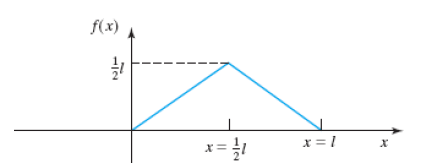
\includegraphics[width=0.6\textwidth]{figures/7.1.png}
        \caption{按箱中粒子函数展开的函数。}
        \label{fig:7.1}
    \end{figure}

    在(\ref{eq:7.33})中将$m$替换为$n$并带入到(\ref{eq:7.29})中,我们得到
    \begin{equation}
        f\left(x\right) = \sum_{n=1}^{\infty} \left[\int_{0}^{l} \psi_n^{\ast} f\left(x\right) \: \mathrm{d}x\right] \psi_n\left(x\right)
        \label{eq:7.34}
    \end{equation}
    这是任意函数 $f\left(x\right)$ 作为箱中粒子波函数 $\psi_n$ 的线性组合的展开所需的表达式。注意:定积分$\int_{0}^{l} \psi_n^{\ast} f\left(x\right) \: \mathrm{d}x$ 是一个数,而不是一个关于$x$的函数。

    我们现在使用(\ref{eq:7.29})来代表一个特定的函数,图(\ref{fig:7.1})所示的函数由下式定义:
    \begin{equation}
        \begin{cases}
            f\left(x\right) = 0, & 0 \leq x < \frac{l}{2} \\
            f\left(x\right) = 1, & \frac{l}{2} \leq x < l
        \end{cases}
        \label{eq:7.35}
    \end{equation}
    为了找到展开系数$a_n$,我们将(\ref{eq:7.35})和(\ref{eq:7.28})代入(\ref{eq:7.33})中:
    \begin{equation*}
        \begin{aligned}
            a_n &= \int_{0}^{l} \psi_n^{\ast} f\left(x\right) \: \mathrm{d}x = \left(\frac{2}{l}\right)^{1/2} \int_{0}^{l} \sin\left(\frac{n\pi x}{l}\right) f\left(x\right) \: \mathrm{d}x \\
            a_n &= \left(\frac{2}{l}\right)^{1/2} \int_{0}^{l/2} x\sin\left(\frac{n\pi x}{l}\right) \: \mathrm{d}x + \left(\frac{2}{l}\right)^{1/2} \int_{l/2}^{l} \left(l-x\right)\sin\left(\frac{n\pi x}{l}\right) \: \mathrm{d}x
        \end{aligned}
    \end{equation*}
    使用附录中的积分A.1,我们得到
    \begin{equation}
        a_n = \frac{\left(2l\right)^{3/2}}{n^2\pi^2}\sin\left(\frac{n\pi}{2}\right)
        \label{eq:7.36}
    \end{equation}
    将(\ref{eq:7.36})代入(\ref{eq:7.29}),我们得到[由于$\sin\left(n\pi/2\right)$在$n$为奇数时为1或-1,在$n$为偶数时为0]:
    \begin{equation*}
        f\left(x\right) = \frac{4l}{\pi^2}\left[\sin\left(\frac{\pi x}{l}\right) - \frac{1}{3^2}\sin\left(\frac{3\pi x}{l}\right) + \frac{1}{5^2}\sin\left(\frac{5\pi x}{l}\right) - \cdots\right]
    \end{equation*}
    \begin{equation}
        f\left(x\right) = \frac{4l}{\pi^2}\sum_{n=1}^{\infty}\left(-1\right)^{n+1}\frac{1}{\left(2n-1\right)^2}\sin\left[\left(2n-1\right)\frac{\pi x}{l}\right]
        \label{eq:7.37}
    \end{equation}
    其中$f\left(x\right)$由(\ref{eq:7.35})给出。让我们检查$x = \frac{1}{2}l$时(\ref{eq:7.37})的值:
    \begin{equation}
        f\left(\frac{l}{2}\right) = \frac{4l}{\pi^2}\left(1+\frac{1}{3^2}+\frac{1}{5^2}+\frac{1}{7^2}+\cdots\right)
        \label{eq:7.38}
    \end{equation}
    将 (\ref{eq:7.38}) 的右边作为我们在无穷级数中所取项数的函数列表,我们可以得到
    \begin{table}[h!]
        \centering
        \begin{tabular}{c|c|c|c|c|c|c|c}
            项数 & 1 & 2 & 3 & 4 & 5 & 20 & 100 \\
            \hline
            式(\ref{eq:7.38})的右侧 & $0.405l$ & $0.450l$ & $0.467l$ & $0.475l$ & $0.480l$ & $0.495l$ & $0.499l$
        \end{tabular}
    \end{table}
    \begin{figure}[h!]
        \centering
        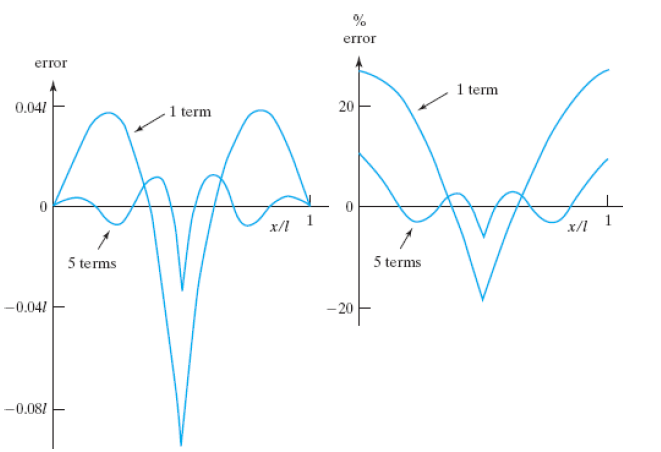
\includegraphics[width=0.6\textwidth]{figures/7.2.png}
        \caption{
            \centering
            \parbox{\linewidth}{
                \centering
                图 \ref{fig:7.1} 中以粒子箱中波函数展开的函数,展开式分别\\
                取 1 项和 5 项时,(a) 误差和(b) 百分比误差图。
            }
        }
        \label{fig:7.2}
    \end{figure}

    \noindent 如果我们取无穷多项,那么级数的和应为$\frac{1}{2}l$,与$f\left(\frac{l}{2}\right)$的值一致。假设级数成立,我们会得到一个有趣的结果,即(\ref{eq:7.38})中右侧括号的求和等于$\pi^2/8$。图7.2显示了$f\left(x\right) - \sum_{n-1}^{k}a_n\psi_n$的图形[其中$f$、$a_n$和$\psi_n$的定义见(\ref{eq:7.35})、(\ref{eq:7.36})和(\ref{eq:7.28})],其中$k$是取的项数,分别为1和5。随着 $k$(即展开式中的项数)的增加,级数逐渐趋近于 $f\left(x\right)$,而 $f$ 与级数之间的差值逐渐趋于零。

\subsection*{用本征函数展开函数}

     我们已经看到了用一组函数——箱中粒子能量本征函数——来展开一个函数的例子。我们可以使用许多不同的函数集来展开任意函数。如果每个品优函数 $f$ 都服从与 $g_i$ 函数相同的边界条件,并且可以根据以下条件展开为 $g_i$ 的线性组合,则称函数集 $g_1,g_2,\ldots,g_i,\ldots$ 为\textbf{完备集}(complete set):
    \begin{equation}
        f = \sum_{i}a_i g_i
        \label{eq:7.39}
    \end{equation}
    其中 $a_i$ 是常数。当然,我们很容易理解$f$和$g_i$都是同一组自变量的函数。(\ref{eq:7.39}) 中的和省略了极限。不言而喻,这个和包含了完整集合的所有成员。根据Fourier分析定理(我们尚未证明),可以证明粒子箱中的能量本征函数是一个完备集。

    我们现在假设:\textit{表示物理量的每个厄米算符的本征函数集是一个完备集。}(本征函数的完备性在很多情况下都可以证明,但在一般情况下必须假设。)因此,每个满足与本征函数集合相同边界条件的品优函数都可以根据 (\ref{eq:7.39}) 展开。方程 (\ref{eq:7.29}) 就是 (\ref{eq:7.39}) 的一个例子。

    谐振子波函数由厄米多项式$H_v$乘以一个指数因子给出[问题4.21c的式(4.86)]。根据展开公设,任何品优函数 $f\left(x\right)$ 都可以展开为谐振子能量本征函数的线性组合:
    \begin{equation*}
        f\left(x\right) = \sum_{n=0}^{\infty}a_n\left(2^nn!\right)^{-1/2}\left(\alpha/\pi\right)^{1/4}H_n\left(\alpha^{1/2}x\right)\mathrm{e}^{-\alpha x^2/2}
    \end{equation*}

    使用氢原子束缚态波函数来展开任意函数 $f\left(r,\theta,\phi\right)$如何?答案是这些函数并\textit{不}构成一个完备集,我们无法用它们来展开 $f$。要有一个完备集,我们必须使用特定厄米算符的\textit{所有}本征函数。除了氢原子哈密顿的束缚态本征函数外,我们还有与电离态相对应的连续态本征函数。如果将连续本征函数与束缚态本征函数一起包含在内,那么我们就得到了一个完备集。(对于箱中粒子和谐振子来说,连续函数不存在。)等式 (\ref{eq:7.39}) 意味着对连续本征函数(如果有的话)进行积分。因此,若$\psi_{nlm}\left(r,\theta,\phi\right)$是氢原子束缚态函数,$\psi_{Elm}\left(r,\theta,\phi\right)$是连续本征函数,则式(\ref{eq:7.39})变为
    \begin{equation*}
        f\left(r,\theta,\phi\right) = \sum_{n=1}^{\infty}\sum_{l=0}^{n-1}\sum_{m=-l}^{l}a_{nlm}\psi_{nlm}\left(r,\theta,\phi\right) + \sum_{l=0}^{\infty}\sum_{m=-l}^{l}\int_{0}^{\infty} a_{lm}\left(E\right) \psi_{Elm}\left(r,\theta,\phi\right) \:\mathrm{d}E
    \end{equation*}

    另一个例子:考虑算符$\hat{p}_x$的本征函数[式(\ref{eq:3.36})]:
    \begin{equation*}
        g_k = \mathrm{e}^{\mathrm{i}kx/\hbar}, \quad -\infty < k < \infty
    \end{equation*}
    这里的本征值都是连续的,任意函数 $f$ 的本征函数展开式(\ref{eq:7.39})变为
    \begin{equation*}
        f\left(x\right) = \int_{-\infty}^{\infty} a\left(k\right) \mathrm{e}^{\mathrm{i}kx/\hbar} \:\mathrm{d}k
    \end{equation*}
    具有良好数学基础的读者可能会发现,这个积分几乎就是 $a\left(k\right)$ 的Fourier变换。

    让我们对$f=\sum_{i}a_ig_i$ [式 (\ref{eq:7.39}) ] 中的展开系数进行计算,其中的 $g_i$ 函数是厄米算符的本征函数的完备集。这一过程与推导 (\ref{eq:7.33}) 所用的过程相同。我们将$f = \sum_{i}a_ig_i$与$g_k^{\ast}$相乘并对全空间积分:
    \begin{equation*}
        g_k^{\ast} f = \sum_{i} a_i g_k^{\ast} g_i
    \end{equation*}
    \begin{equation*}
        \int g_k^{\ast} f \:\mathrm{d}\tau = \sum_{i} a_i \int g_k^{\ast} g_i \:\mathrm{d}\tau = \sum_{i} a_i \delta_{ik} = a_k
    \end{equation*}
    \begin{equation}
        a_k = \int g_k^{\ast} f \:\mathrm{d}\tau
        \label{eq:7.40}
    \end{equation}
    其中我们用到了厄米算符本征函数之间的正交性:$\int g_k^{\ast} g_i \:\mathrm{d}\tau = \delta_{ik}$ [式 (\ref{eq:7.26}) ]。得出(\ref{eq:7.40})的过程会经常用到,值得记住。将(\ref{eq:7.40})中的$a_i$带入$f = \sum_{i}a_ig_i$中,我们得到
    \begin{equation}
        f = \sum_{i}\left[\int g_i^{\ast}f \:\mathrm{d}\tau\right]g_i = \sum_{i}\left\langle g_i \middle| f \right\rangle g_i
        \label{eq:7.41}
    \end{equation}

    \begin{examplebox}
        \textbf{例题:}令
        \begin{equation*}
            F\left(x\right) = \begin{cases}
                x\left(l-x\right), & 0 \leq x \leq l \\
                0, & \text{elsewhere}
            \end{cases}
        \end{equation*}
        将$F$用箱中粒子能量本征函数$\psi_n = \left(2/l\right)^{1/2}\sin\left(n\pi x/l\right), \: 0 \leq x \leq l$展开。
        \\
        
        注意到$F\left(0\right) = 0$以及$F\left(l\right) = 0$,因此满足与$\psi_n$相同的边界条件。我们可以使用$\psi_n$来展开$F$。展开式为$F = \sum_{n=1}^{\infty} a_n \psi_n$,其中系数$a_n = \int\psi_n^{\ast} F \:\mathrm{d}x$[式(\ref{eq:7.40})和(\ref{eq:7.39})]。因此,
        \begin{equation*}
            a_n = \int \psi_{n}^{\ast}F \:\mathrm{d}\tau = \left(\frac{2}{l}\right)^{1/2} \int_{0}^{l} \left(\sin\frac{n\pi x}{l}\right) x\left(l-x\right) \:\mathrm{d}x = \frac{2^{3/2}l^{5/2}}{n^3\pi^3}\left[1-\left(-1\right)^n\right]
        \end{equation*}
        其中积分计算的具体细节留作习题(问题7.18)。展开式$F = \sum_{n=1}^{\infty} a_n \psi_n$为
        \begin{equation*}
            x\left(l-x\right) = \frac{4l^2}{\pi^3}\sum_{n=1}^{\infty} \frac{1-\left(-1\right)^n}{n^3}\sin\left(\frac{n\pi x}{l}\right), \quad 0 \leq x \leq l
        \end{equation*}
        \\

        \textbf{练习:}令
        \begin{equation*}
            G\left(x\right) = \begin{cases}
                1, & 0 \leq x \leq l \\
                0, & \text{elsewhere}
            \end{cases}
        \end{equation*}
        将$G$用箱中粒子能量本征函数展开。由于 $G$ 在 原点和 $l$ 点不为零,因此展开式在这些点上不表示 $G$,而在其他地方表示 $G$。利用展开式的前 7 项非零项计算 $G$ 在$x = \frac{1}{4}l$处的值。使用前 70 个非零项重复上述步骤(使用可编程计算器)。(\textit{答案:}0.1219,0.9977.)
    \end{examplebox}

    以下是一条有用的定理:
    \begin{center}
        \parbox{0.8\textwidth}{
            \centering
            \textbf{定理3:}令$g_1,g_2,\ldots$是厄米算符$\hat{A}$的本征函数完备集,令$F$是$\hat{A}$的本征函数,本征值为$k$(也就是说,$\hat{A}F = kF$)。若$F$展开为$F = \sum_{i}a_ig_i$,则展开式中的非零系数$a_i$仅对应于与$k$相同的本征值的本征函数$g_i$。(由于简并的存在,可能有多个本征函数$g_i$对应于同一本征值$k$。)
            
        }
    \end{center}

    因此,在 $F$ 的展开式中,我们只包括那些与 $F$ 具有相同本征值的本征函数。根据 $a_k = \int g_k^{\ast} f \:\mathrm{d}\tau$[公式 (\ref{eq:7.40}) ] 即可得出定理 3 的证明;若$F$和$g_i$对应于同一厄米算符$\hat{A}$的不同本征值,那它们是正交的[式(\ref{eq:7.22})],则$a_k$消失。

    我们偶尔会使用一种符号(称为 \textbf{ket} 符号),在这种符号中,函数 $f$ 用以下符号表示$\left| f \right\rangle$。这个符号似乎没有任何意义,但在量子力学的高级公式中,它具有特殊的意义。在ket符号中,式(\ref{eq:7.41})可以写成
    \begin{equation}
        \left| f \right\rangle = \sum_{i} \left| g_i\right\rangle \left\langle g_i \middle| f \right\rangle = \sum_i \left| i \right\rangle \left\langle i \middle| f \right\rangle
        \label{eq:7.42}
    \end{equation}
    Ket 符号方便地用于通过列出本征值来指定本征函数。例如,量子数分别为$n$、$l$和$m$的氢原子波函数可以写成$\psi_{nlm} = \left| n,l,m \right\rangle$。

    第\ref{sec:7.2 Hermitian Operators}和\ref{sec:7.3 Expansion in Terms of Eigenfunctions}节的内容可以总结为\textit{厄米算符的本征函数构成一个完整的正交集合,且本征值为实数。}

\section{对易算符的本征函数}
\label{sec:7.4 Eigenfunctions of Commuting Operators}










\section{宇称}
\label{sec:7.5 Parity}

\section{测量和态叠加}
\label{sec:7.6 Measurement and the Superposition of States}

\section{坐标本征函数}
\label{sec:7.7 Position Eigenfunctions}

\section{量子力学的基本假设}
\label{sec:7.8 The Postulates of Quantum Mechanics}

\section{测量和量子力学解释}
\label{sec:7.9 Measurement and the Interpretation of Quantum Mechanics}

\section{矩阵}
\label{sec:7.10 Matrices}

\section*{总结}

\section*{习题}
	
	% ===== CHAPTER 8 =====
\chapter{变分法}
\label{chap:8}
\section{变分理论}
\label{sec:8.1 The Variation Theorem}
    为了处理包含相互作用粒子系统(如原子和分子)的定态薛定谔方程,我们必须使用近似方法。本章讨论变分法,它允许我们在不求解薛定谔方程的情况下近似得到系统的基态能量。变分法基于如下理论:
    \begin{center}
        \parbox{0.8\textwidth}{
            \textbf{变分理论:}
            
            给定一个系统,其哈密顿算符$\hat{H}$与时间无关,其最低能量本征值为$E_1$,如果 $\phi$ 是系统粒子坐标的任何满足问题定解条件的已归一化品优函数,那么
            \begin{equation}
                \boxed{
                    \int \phi^{\ast}\hat{H}\:\mathrm{d}\tau \geq E_1, \quad \phi \text{已归一化}
                }
                \label{eq:8.1}
            \end{equation}
        }
    \end{center}

    变分理论允许我们计算系统基态能量的最大值。

    为了证明(\ref{eq:8.1}),我们将$\phi$用$\hat{H}$的本征函数完全正交集,即定态本征函数$\psi_k$展开:
    \begin{equation}
        \phi = \sum_k a_k \psi_k
        \label{eq:8.2}
    \end{equation}
    其中
    \begin{equation}
        \hat{H}\psi_k = E_k \psi_k
        \label{eq:8.3}
    \end{equation}
    注意:展开式(\ref{eq:8.2})要求$\phi$满足与$\psi_k$相同的定解条件。将(\ref{eq:8.2})代入(\ref{eq:8.1})的左侧,我们得到
    \begin{equation*}
        \int \phi^{\ast}\hat{H}\phi\:\mathrm{d}\tau = \int \sum_{k}a_k^{\ast} \psi_k^{\ast} \hat{H} \sum_{j} a_j \psi_j \:\mathrm{d}\tau = \int \sum_{k}a_k^{\ast} \psi_k^{\ast} \sum_{j} a_j \hat{H} \psi_j \:\mathrm{d}\tau
    \end{equation*}
    利用本征方程 (\ref{eq:8.3}),并假设交换积分和无限求和是成立的,我们可以得到
    \begin{equation*}
        \begin{aligned}
            \int \phi^{\ast}\hat{H}\phi \:\mathrm{d}\tau &= \int \sum_{k} a_k^{\ast} \psi_k^{\ast} \hat{H} \sum_{j} a_j \psi_j \:\mathrm{d}\tau = \int \sum_{k} a_k^{\ast} \psi_k^{\ast} \sum_{j} a_j \hat{H} \psi_j \:\mathrm{d}\tau \\
            &= \sum_k\sum_{j} a_k^{\ast} a_j E_j \delta_{kj}
        \end{aligned}
    \end{equation*}
    其中用到了本征函数$\psi_k$的正交性。我们对 $j$ 求和,像往常一样,除了 $j=k$ 的项之外,Kronecker $\delta$使所有项都为零,从而得到
    \begin{equation}
        \int \phi^{\ast} \hat{H}\phi \:\mathrm{d}\tau = \sum_{k}a_k^{\ast} a_k E_k = \sum_k |a_k|^2 E_k
        \label{eq:8.4}
    \end{equation}
    
    由于$E_1$是$\hat{H}$的最低能量本征值,我们有$E_k \geq E_1$,又由于$\left|a_k\right|^2$为非负数,我们可以将不等式$E_k \geq E_1$的左右两侧乘以$|a_k|^2$而不改变不等号的方向,从而得到$|a_k|^2 E_k \geq |a_k|^2 E_1$。因此,$\sum_k |a_k|^2 E_k \geq \sum_k |a_k|^2 E_1$,使用(\ref{eq:8.4}),我们得到
    \begin{equation}
        \int \phi^{\ast} \hat{H}\phi \:\mathrm{d}\tau = \sum_k |a_k|^2 E_k \geq \sum_k |a_k|^2 E_1 = E_1 \sum_k |a_k|^2
        \label{eq:8.5}
    \end{equation}

    因为$\phi$已归一化,我们有$\int \phi^{\ast} \phi \: \mathrm{d}\tau = 1$。将展开式(\ref{eq:8.2})代入归一化条件,得到
    \begin{equation*}
        1 = \int \phi^{\ast} \phi \: \mathrm{d}\tau = \int \sum_{k} a_k^{\ast} \psi_k^{\ast} \sum_{j} a_j \psi_j \: \mathrm{d}\tau = \sum_{k} \sum_{j} a_k^{\ast} a_j \int \psi_k^{\ast} \psi_j \: \mathrm{d}\tau = \sum_{k} \sum_{j} a_k^{\ast} a_j \delta_{kj}
    \end{equation*}
    \begin{equation}
        1 = \sum_{k} |a_k|^2
        \label{eq:8.6}
    \end{equation}
    [注意,在推导公式 (\ref{eq:8.4}) 和 (\ref{eq:8.6}) 时,我们基本上分别重复了公式 (\ref{eq:7.70}) 和 (\ref{eq:7.69}) 的推导。]

    将(\ref{eq:8.6}) 代入 (\ref{eq:8.5})就得到了变分理论(\ref{eq:8.1})的证明:
    \begin{equation}
        \int \phi^{\ast} \hat{H}\phi \:\mathrm{d}\tau \geq E_1, \quad \phi \text{已归一化}
        \label{eq:8.7}
    \end{equation}

    假设我们有一个未归一化的函数$\phi$。为了应用变分理论,我们用一个归一化常数$N$乘以$\phi$使得$N\phi$满足归一化条件。在(\ref{eq:8.7})中,我们将$\phi$替换为$N\phi$,得到
    \begin{equation}
        \left|N\right|^2 \int \phi^{\ast} \hat{H}\phi \:\mathrm{d}\tau \geq E_1
        \label{eq:8.8}
    \end{equation}
    $N$由下式导出:$\int \left(N\phi\right)^{\ast} \left(N\phi\right) \:\mathrm{d}\tau = \left|N\right|^2 \int \phi^{\ast} \phi \:\mathrm{d}\tau = 1$,因此$\left|N\right|^2 = 1/\int \phi^{\ast} \phi \:\mathrm{d}\tau$。将其代入(\ref{eq:8.8}),我们得到
    \begin{equation}
        \boxed{
            \frac{\int \phi^{\ast} \hat{H}\phi \:\mathrm{d}\tau}{\int \phi^{\ast} \phi \:\mathrm{d}\tau} \geq E_1
        }
        \label{eq:8.9}
    \end{equation}
    其中$\phi$是满足问题定解条件的任意品优函数(不必归一化)。

    函数$\phi$称为\textbf{试探变分函数}(trial variational function),(\ref{eq:8.1})中的积分[或 (\ref{eq:8.9}) 中的积分之比]称为\textbf{变分积分}(variational integral)。为了获取基态能量$E_1$的良好近似值,我们会尝试许多试探变分函数,并寻找能给出最小变分积分值的函数。由 (\ref{eq:8.1}) 可知,变分积分的值越小,我们对 $E_1$ 的近似就越好。推翻量子力学的一种方法是找到一个试探变分函数,使已知 $E_1$ 的某个系统的变分积分小于 $E_1$。

    令$\psi_1$为系统基态能量的真实波函数:
    \begin{equation}
        \hat{H}\psi_1 = E_1 \psi_1
        \label{eq:8.10}
    \end{equation}
    如果我们碰巧幸运地发现了一个等于 $\psi_1$ 的变分函数,那么在 (\ref{eq:8.1}) 中使用 (\ref{eq:8.10}) ,我们可以看到变分积分将等于 $E_1$。因此,基态波函数给出了变分积分的最小值。因此,我们预期变分积分值越小,试探变分函数就越接近真实的基态波函数。然而,事实证明,变分积分接近 $E_1$ 的速度要比试探变分函数接近 $\psi_1$ 的速度快得多,而且有可能用一个相当差的 $\phi$ 得到一个相当好的近似值 $E_1$。

    在实践中,人们通常会在试探函数 $\phi$ 中引入几个参数,然后对这些参数进行变分,从而使变分积分最小化。能否成功使用变分法,取决于能否对试探函数做出正确的选择。

    让我们来看一些变分法的例子。虽然这种方法的真正用途是针对我们不知道确切解的问题,但我们还是要考虑那些完全可解的问题,以便判断我们结果的准确性。

    \begin{examplebox}
        \textbf{例题:}为长度为 $l$ 的一维势箱中的粒子设计一个试探变分函数。
        \\

        波函数在势箱外为零,定解条件要求在$x=0$和$x=l$处$\psi=0$。变分函数$\phi$必须满足这些在边界点为零的条件。如公式 (\ref{eq:4.57}) 后所述,基态 $\psi$ 在边界点内部没有节点,因此希望 $\phi$ 也没有内部节点。具有这些性质的一个简单函数为抛物线函数
        \begin{equation}
            \phi = x\left(l-x\right), \quad 0 \leq x \leq l
            \label{eq:8.11}
        \end{equation}
        以及在势箱外,有$\phi=0$。由于我们尚未归一化$\phi$,我们使用(\ref{eq:8.9})来计算。势箱内部的哈密顿算符为$-\left(\hbar^2/2m\right)\mathrm{d}^2/\mathrm{d}x^2$。对于 (\ref{eq:8.9}) 的分子和分母,我们可以得出
        \begin{equation}
            \int \phi^{\ast} \hat{H}\phi \:\mathrm{d}\tau = -\frac{\hbar^2}{2m} \int_{0}^{l} \left(lx-x^2\right)\frac{\mathrm{d}^2}{\mathrm{d}x^2} \left(lx-x^2\right) \mathrm{d}x = \frac{\hbar^2}{m} \int_0^l \left(lx-x^2\right) \:\mathrm{d}x = \frac{\hbar^2 l^3}{6m}
            \label{eq:8.12}
        \end{equation}
        \begin{equation}
            \int \phi^{\ast} \phi \:\mathrm{d}\tau = \int_0^l x^2\left(l-x\right)^2 \:\mathrm{d}x = \frac{l^5}{30}
            \label{eq:8.13}
        \end{equation}
        将它们带入变分理论(\ref{eq:8.9}),我们得到
        \begin{equation*}
            E_1 \leq \frac{5h^2}{4\pi^2 ml^2} = 0.1266515\frac{\hbar^2}{ml^2}
        \end{equation*}
        根据(\ref{eq:2.20 energy of one-dimensional box}),$E_1$的准确值为$h^2/8ml^2=0.125h^2/8ml^2$,能量的误差约为$1.3\%$。

        由于$\int \left|\phi\right|^2 \: \mathrm{d}\tau = l^5/30$,将(\ref{eq:8.11})归一化为$\left(30/l^5\right)^{1/2} x\left(l-x\right)$。图\ref{fig:7.3}显示,该函数与真正的箱中粒子基态波函数非常相似。
        \\

        \textbf{练习:}一个单粒子一维系统的势能函数满足
        \begin{equation*}
            V = \begin{cases}
                V_0, & 0 \leq x \leq l \\
                \infty, & elsewhere
            \end{cases}
        \end{equation*}
        (其中$V_0$是常数)。

        (a)使用试探函数
        \begin{equation*}
            \phi = \begin{cases}
                \sin\left(\pi x/l\right), & 0 \leq x \leq l \\
                0, & elsewhere
            \end{cases}
        \end{equation*}
        来估算该系统的基态能量;

        (b)解释为什么(a)的结果是该系统的准确基态能量。\textit{提示:见第\ref{chap:4}章的问题之一。}(答案:(a)$V_0 + h^2/8ml^2$。)
    \end{examplebox}

    上一个例题的试探函数中没有参数。下一个例题有。

    \begin{examplebox}
        \textbf{例题:}对于一维谐振子,设计一个带有参数的变分函数,并找出参数的最佳值。估计基态能量。
        \\

        变分函数$\phi$必须平方可积,即当$x \to \pm \infty$时,$\phi \to 0$。函数$\mathrm{e}^{-x}$在$+ \infty$时满足条件,但在$-\infty$时变为无穷大。函数$\mathrm{e}^{-x^2}$在$\pm \infty$时都满足条件。然而,从量纲上看,这种做法并不令人满意,因为$\mathrm{e}$的指数必须是无量纲的。这可以从Taylor级数中看出$\mathrm{e}^z = 1 + z + z^2/2! + z^3/3! + \ldots$[式(\ref{eq:4.44})]。由于该级数中的所有项都必须有相同的量纲,那么$z$的量纲就必须为1,也就是说$\mathrm{e}^z$中的$z$必须是无量纲的。因此,我们将$\mathrm{e}^{-x^2}$替换为$\mathrm{e}^{-cx^2}$,其中$c$的量纲为长度$^{-2}$。我们将$c$作为变分参数。真实的基态$\psi$没有节点。此外,由于$V = \frac{1}{2}kx^2$是偶函数,由于奇函数在原点有节点,那么基态的$\psi$一定具有确定的宇称,也一定是偶函数。试探函数$\mathrm{e}^{-cx^2}$具有我们需要的性质:无节点,且为偶函数。

        对$\hat{H}$使用(\ref{eq:4.30}),再使用附录中的积分,有(问题8.3)
        \begin{equation*}
            \begin{aligned}
                \int \phi^{\ast} \hat{H}\phi \:\mathrm{d}\tau &= -\frac{\hbar^2}{2m} \int_{-\infty}^{\infty} \mathrm{e}^{-2cx^2} \frac{\mathrm{d}^2\mathrm{e}^{-cx^2}}{\mathrm{d}x^2} \:\mathrm{d}x + 2\pi^2\nu^2m\int_{-\infty}^{\infty} x^2 \mathrm{e}^{-2cx^2} \:\mathrm{d}x \\
                &= \frac{\hbar^2}{m} \left(\frac{\pi c}{m}\right)^{1/2} + \nu^2m\left(\frac{\pi^5}{8}\right)^{1/2} c^{-3/2}
            \end{aligned}
        \end{equation*}
        \begin{equation*}
            \int \phi^{\ast} \phi \:\mathrm{d}\tau = \int_{-\infty}^{\infty} \mathrm{e}^{-2cx^2} \:\mathrm{d}x = 2\int_{0}^{\infty} \mathrm{e}^{-2cx^2} \:\mathrm{d}x = \left(\frac{\pi}{2c}\right)^{1/2}
        \end{equation*}
        试探积分$W$为
        \begin{equation}
            W \equiv \frac{\int \phi^{\ast} \hat{H}\phi \:\mathrm{d}\tau}{\int \phi^{\ast} \phi \:\mathrm{d}\tau} = \frac{\hbar^2c}{2m} + \frac{\pi^2\nu^2m}{2c}
            \label{eq:8.14}
        \end{equation}
        现在,我们通过改变$c$来最小化$W$(\ref{eq:8.14})。$W$最小的必要条件为
        \begin{equation*}
            \frac{\mathrm{d} W}{\mathrm{d} c} = 0 = \frac{\hbar^2}{2m} - \frac{\pi^2\nu^2m}{2c^2}
        \end{equation*}
        \begin{equation}
            c = \pm \pi \nu m/\hbar
            \label{eq:8.15}
        \end{equation}
        其中,负根$c = -\pi\nu m/\hbar$应舍去,因其会导致$\phi = \mathrm{e}^{-cx^2}$不满足平方可积的要求。将$c = \pi\nu m/\hbar$代入(\ref{eq:8.14}),我们得到$W = \frac{1}{2}h\nu$。这是一维谐振子基态能量的准确值。当$c = \pi\nu m/\hbar$时,变分函数$\phi$除了未归一化以外,与谐振子基态波函数(\ref{eq:4.53})和(\ref{eq:4.31})完全一致。

        对于归一化的谐振子变分函数$\phi = \left(2c/\pi\right)^{1/4} \mathrm{e}^{-cx^2}$,若$c$的值很大,会导致$\phi$在$x=0$附近从其最大值快速下降。那么概率密度就只在$x=0$附近较大。势函数$V = \frac{1}{2}kx^2$在$x=0$附近也很小,所以较大的$c$值意味着较小的$\left\langle V \right\rangle = \left\langle \phi \middle| V \middle| \phi \right\rangle$。[注意:$\left\langle V \right\rangle$等于(\ref{eq:8.14})右侧的第二项。]然而,由于较大的$c$值使得$\phi$从其最大值快速减小,那么在$x=0$附近$\left|\mathrm{d}\phi/\mathrm{d}x\right|$的值变得很大,根据问题7.7b,大$\left|\mathrm{d}\phi/\mathrm{d}x\right|$意味着大$\left\langle T \right\rangle$[等于(\ref{eq:8.14})右侧的第一项。]$c$的最佳值可以使总和$\left\langle T \right\rangle + \left\langle V \right\rangle = W$最小化。在原子和分子中,真正的波函数是通过将电子限制在低$V$区域(靠近原子核)来最小化$\left\langle V \right\rangle$的趋势与通过允许电子概率密度在大区域内扩散来最小化$\left\langle T \right\rangle$的趋势之间的折衷。
        \\

        \textbf{练习:}考虑一个单粒子一维系统,其势函数满足
        \begin{equation*}
            V = \begin{cases}
                V = 0, & -\frac{1}{2}l \leq x \leq \frac{1}{2}l \\
                V = b\hbar^2/ml^2, & elsewhere
            \end{cases}
        \end{equation*}
        其中$b$是正常数(图 \ref{fig:2.5} 中的 $V_0 = b\hbar^2/ml^2$ 和原点发生了偏移)。

        (a)对于变分函数
        \begin{equation*}
            \phi = \begin{cases}
                \left(x-c\right)\left(x+c\right) = x^2 - c^2, & -c \leq x \leq c \\
                0, & elsewhere
            \end{cases}
        \end{equation*}
        其中变分参数$c > \frac{1}{2}l$。我们发现变分积分$W$由下式给出:
        \begin{equation*}
            W = \frac{\hbar^2}{ml^2}\left[\frac{5l^2}{4c^2} + b\left(1-\frac{15l}{16c} + \frac{5l^3}{32c^3} - \frac{3l^5}{256c^5}\right)\right]
        \end{equation*}
        在同一幅图上绘制$\phi$和$V$的图象。求使 $W$ 最小的 $c$ 值所满足的方程。

        (b)当$V_0 = 20\hbar^2/ml^2$时,求出$c$的最佳值和$W$的值,将其与基态能量真实值$2.814\hbar^2/ml^2$进行比较(问题4.31c)。(\textit{提示:}可以使用Excel表格求解器或可编程计算器来计算$c/l$的值。)

        (\textit{答案:}(a)$48t^4-24t^2-128t^3/b+3=0$,其中$t \equiv c/l$;(b)$c = 0.6715l$,$W = 3.454\hbar^2/ml^2$。)
    \end{examplebox}

\section{变分法的推广}
\label{sec:8.2 Extension of the Variational Method}
    上一节介绍的变分法只提供了基态能量和波函数的信息。现在我们讨论将变分法推广到激发态。(另请参见第 \ref{sec:8.5 Linear Variational Functions} 节)。

    考虑一下我们可以如何推广变分法,来估算第一激发态的能量。根据能量从低到高:
    \begin{equation*}
        E_1 \leq E_2 \leq E_3 \leq \ldots
    \end{equation*}
    我们将系统的状态标号为$1,2,3,\ldots$。我们已经证明:对于一个已归一化的变分函数$\phi$,有[式(\ref{eq:8.4})和(\ref{eq:8.6})]
    \begin{equation*}
        \int \phi^{\ast} \hat{H}\phi \:\mathrm{d}\tau = \sum_{k=1}^{\infty} |a_k|^2 E_k \quad \text{和} \quad \int \phi^{\ast} \phi \:\mathrm{d}\tau = \sum_{k=1}^{\infty} |a_k|^2 = 1
    \end{equation*}
    其中的$a_k$是展开式$\phi = \sum_{k} a_k \psi_k$中的系数[式(\ref{eq:8.2})]。我们有$a_k = \left\langle \psi_k \middle| \phi \right\rangle$[式(\ref{eq:7.40})]。让我们只讨论与真实基态波函数$\psi$正交的归一化函数$\phi$。那么$a_1 = \left\langle \psi_1 \middle| \phi \right\rangle = 0$,因此
    \begin{equation}
        \int \phi^{\ast} \hat{H}\phi \:\mathrm{d}\tau = \sum_{k=2}^{\infty} |a_k|^2 E_k \quad \text{和} \quad \int \phi^{\ast} \phi \:\mathrm{d}\tau = \sum_{k=2}^{\infty} |a_k|^2 = 1
        \label{eq:8.16}
    \end{equation}
    对于$k \geq 2$,我们有$E_k \geq E_2$和$\left|a_k\right|^2E_k \geq \left|a_k\right|^2E_2$。因此,
    \begin{equation}
        \sum_{k=2}^{\infty} \left|a_k\right|^2 E_k \geq \sum_{k=2}^{\infty} \left|a_k\right|^2 E_2 = E_2 \sum_{k=2}^{\infty} \left|a_k\right|^2 = E_2
        \label{eq:8.17}
    \end{equation}
    将(\ref{eq:8.16})和(\ref{eq:8.17})相结合,我们得到了所需的结果:
    \begin{equation}
        \int \phi^{\ast} \hat{H}\phi \:\mathrm{d}\tau \geq E_2, \quad \text{若} \int \psi^{\ast} \phi \:\mathrm{d}\tau = 0 \quad \text{且} \int \phi^{\ast} \phi \:\mathrm{d}\tau = 1
        \label{eq:8.18}
    \end{equation}
    通过不等式 (\ref{eq:8.18}) 我们可以得到第一激发态的能量 $E_2$ 的上限。然而,限制条件$\left\langle \psi_1 \middle| \phi \right\rangle = 0$使得这种方法在应用上会很麻烦。

    对于特定的系统,尽管我们不知道真实基态波函数,但确定$\left\langle \psi_1 \middle| \phi \right\rangle = 0$是可能的。$V$ 是 $x$ 的偶函数的一维问题就是一个例子。在这种情况下,基态波函数总是偶函数,而第一激发态波函数是奇函数。(所有波函数必须具有确定的宇称。基态波函数是无节点的,由于奇函数在原点消失,所以基态波函数必须是偶函数。第一个激发态波函数有一个节点,一定是奇函数。)因此,对于奇函数,$\left\langle \psi_1 \middle| \phi \right\rangle = 0$一定成立,偶函数$\psi_1$乘以一个奇函数$\phi$得到一个奇被积函数,从$-\infty$到$+\infty$的积分为零。

    另一个例子是在中心场中运动的粒子(第 \ref{sec:6.1 The One-Particle Central Force Problem} 节)。势能的形式可能使我们无法求解本征函数中的径向因子 $R(r)$。然而,其中的角度因子 $\psi$ 是球谐函数[式 (\ref{eq:6.16}) ],而不同 $l$ 值的球谐函数是正交的。因此,我们可以利用试探函数中的因子$Y_l^m$,求出任意给定角动量$l$的最低态能量上限。这一结果取决于将 (\ref{eq:8.18}) 推广到更高的激发态:
    \begin{equation}
        \frac{\int \phi^{\ast} \hat{H}\phi \:\mathrm{d}\tau}{\int \phi^{\ast} \phi \:\mathrm{d}\tau} \geq E_{k+1}, \quad \text{若} \int \psi_1^{\ast} \phi \: \mathrm{d}\tau = \int \psi_2^{\ast} \phi \:\mathrm{d}\tau = \cdots = \int \psi_k^{\ast} \phi \:\mathrm{d}\tau = 0
        \label{eq:8.19}
    \end{equation}

\section{行列式}
\label{sec:8.3 Determinants}
    第 \ref{sec:8.5 Linear Variational Functions} 节讨论了一种变分函数,它产生了一个涉及行列式的方程。因此,我们现在讨论行列式。
     
    \textbf{行列式}(Determinant)是一个包含 $n^2$ 个量(称为\textbf{元素}(elements))的正方形数组;行列式的值是根据其元素计算出来的,计算方法稍后给出。$n$称为行列式的\textbf{阶}(order)。使用$a_{ij}$来代表一个典型元素,我们有$n$阶行列式
    \begin{equation}
            \det\left(a_{ij}\right) = \begin{vmatrix}
                a_{11} & a_{12} & a_{13} & \cdots & a_{1n} \\
                a_{21} & a_{22} & a_{23} & \cdots & a_{2n} \\
                \vdots & \vdots & \vdots & \ddots & \vdots \\
                a_{n1} & a_{n2} & a_{n3} & \cdots & a_{nn}
            \end{vmatrix}
            \label{eq:8.20}
    \end{equation}
    (\ref{eq:8.20})中的竖线与绝对值无关。在考虑$n$阶行列式值的定义方法之前,我们先考虑一阶、二阶和三阶行列式。

    一阶行列式有一个元素,其值就是该元素本身。因此,
    \begin{equation}
        \left| a_{11} \right| = a_{11}
        \label{eq:8.21}
    \end{equation}
    其中的竖线表示行列式而不是绝对值。

    二阶行列式有四个元素,其值定义为
    \begin{equation}
        \boxed{
            \begin{vmatrix}
                a_{11} & a_{12} \\
                a_{21} & a_{22}
            \end{vmatrix} = a_{11}a_{22} - a_{12}a_{21}
        }
        \label{eq:8.22}
    \end{equation}
    三阶行列式的值定义为
    \begin{equation}
            \boxed{
            \begin{vmatrix}
                a_{11} & a_{12} & a_{13} \\
                a_{21} & a_{22} & a_{23} \\
                a_{31} & a_{32} & a_{33}
            \end{vmatrix} = a_{11}\begin{vmatrix}
                a_{22} & a_{23} \\
                a_{32} & a_{33}
            \end{vmatrix} - a_{12}\begin{vmatrix}
                a_{21} & a_{23} \\
                a_{31} & a_{33}
            \end{vmatrix} + a_{13}\begin{vmatrix}
                a_{21} & a_{22} \\
                a_{31} & a_{32}
            \end{vmatrix}
        }
        \label{eq:8.23}
    \end{equation}
    \begin{equation}
        \begin{aligned}
            = & a_{11}a_{22}a_{33} - a_{11}a_{23}a_{32} - a_{12}a_{21}a_{33} + a_{12}a_{23}a_{31} \\ 
            & + a_{13}a_{21}a_{32} - a_{13}a_{22}a_{31}
        \end{aligned}
        \label{eq:8.24}
    \end{equation}
    三阶行列式的计算方法是:用正负号交替写下第一行的元素,然后将每个元素乘以某个二阶行列式;在三阶行列式中划掉某个元素出现的行和列,就能找到与该元素相乘的二阶行列式。将$n$阶行列式的第$i$行和第$j$列删去后得到的$\left(n-1\right)$阶行列式称为元素$a_{ij}$的\textbf{余子式}(minor)。我们再定义$a_{ij}$的\textbf{代数余子式}(cofactor)为$a_{ij}$的余子式乘以$(-1)^{i+j}$。因此,(\ref{eq:8.23}) 说明三阶行列式的计算方法是:将顶行的每个元素乘以它的代数余子式,然后将三个乘积相加。[注意:式(\ref{eq:8.22})通过代数余子式符合该方法。因为$a_{11}$的代数余子式为$a_{22}$,$a_{12}$的代数余子式为$-a_{21}$。]一个数值的例子如下
    \begin{equation*}
        \begin{aligned}
            \begin{vmatrix}
                5 & 10 & 2 \\
                0.1 & 3 & 1 \\
                0 & 4 & 4
            \end{vmatrix} &= 5\begin{vmatrix}
                3 & 1 \\
                4 & 4
            \end{vmatrix} - 10\begin{vmatrix}
                0.1 & 1 \\
                0 & 4
            \end{vmatrix} + 2\begin{vmatrix}
                0.1 & 3 \\
                0 & 4
            \end{vmatrix} \\
            &= 5\left(8\right) - 10\left(0.4\right) + 2\left(0.4\right) = 36.8
            \end{aligned}
    \end{equation*}

    我们将$a_{ij}$的余子式记为$M_{ij}$,代数余子式记为$C_{ij}$,则
    \begin{equation}
        c_{ij} = \left(-1\right)^{i+j}M_{ij}
        \label{eq:8.25}
    \end{equation}
    则三阶行列式的展开式(\ref{eq:8.23})可以写为
    \begin{equation}
        \det\left(a_{ij}\right) = \begin{vmatrix}
            a_{11} & a_{12} & a_{13} \\
            a_{21} & a_{22} & a_{23} \\
            a_{31} & a_{32} & a_{33}
        \end{vmatrix} = a_{11}C_{11} + a_{12}C_{12} + a_{13}C_{13}
        \label{eq:8.26}
    \end{equation}
    三阶行列式可以用任意一行的元素和相应的代数余子式展开。例如,利用第二行展开三阶行列式,我们可以得出
    \begin{equation}
        \det\left(a_{ij}\right) = a_{21}C_{21} + a_{22}C_{22} + a_{23}C_{23}
        \label{eq:8.27}
    \end{equation}
    \begin{equation}
        \det\left(a_{ij}\right) = -a_{21}\begin{vmatrix}
            a_{11} & a_{13} \\
            a_{31} & a_{33}
        \end{vmatrix} + a_{22}\begin{vmatrix}
            a_{11} & a_{13} \\
            a_{31} & a_{33}
        \end{vmatrix} - a_{23}\begin{vmatrix}
            a_{11} & a_{12} \\
            a_{31} & a_{32}
        \end{vmatrix}
        \label{eq:8.28}
    \end{equation}
    二阶行列式的展开式表明 (\ref{eq:8.28}) 等于 (\ref{eq:8.24})。我们也可以使用任意一列的元素和相应的代数余子式来展开行列式,这一点很容易得到验证。因此,对于三阶行列式,我们可以写成
    \begin{equation*}
        \det\left(a_{ij}\right) = a_{k1}C_{k1} + a_{k2}C_{k2} + a_{k3}C_{k3} = \sum_{l=1}^{3} a_{kl}C_{kl}, \quad k = 1,2,3
    \end{equation*}
    \begin{equation*}
        \det\left(a_{ij}\right) = a_{1k}C_{1k} + a_{2k}C_{2k} + a_{3k}C_{3k} = \sum_{l=1}^{3} a_{lk}C_{lk}, \quad k = 1,2,3
    \end{equation*}
    第一个展开式按某一行展开,第二个则按某一列展开。

    我们通过类似的行(或列)展开来定义高阶行列式。对于 $n$ 阶行列式,
    \begin{equation}
        \det\left(a_{ij}\right) = \sum_{l=1}^{n} a_{kl}C_{kl} = \sum_{l=1}^{n} a_{lk}C_{lk}, \quad k = 1,2,\ldots,n
        \label{eq:8.29}
    \end{equation}

    一些有关行列式的性质如下所述(证明见\textit{Sokolnikoff and Redheffer}, pp. 702–707):
        \begin{enumerate}
            \item 如果行列式某行(或列)的每个元素都为零,则行列式的值为零。
            \item 交换行列式的两行(或两列)会使行列式的值改变符号。
            \item 如果行列式的两行(或两列)相同,则该行列式的值为零。
            \item 如果将行列式的一行(或一列)乘以一个常数 $k$,则该行列式的值也乘以 $k$。
            \item 如在一行的每个元素上加上另一行相应元素的相同常数倍数,行列式的值不变。这个定理也适用于将一列的倍数加到另一列。
            \item 互换所有相应的行和列,行列式的值保持不变。(这种互换意味着第一列变为第一行,第二列变为第二行,等等)
        \end{enumerate}
    
    \begin{examplebox}
        \textbf{例题:}使用性质5计算
        \begin{equation}
            B = \begin{vmatrix}
                1 & 2 & 3 & 4 \\
                4 & 1 & 2 & 3 \\
                3 & 4 & 1 & 2 \\
                2 & 3 & 4 & 1
            \end{vmatrix}
            \label{eq:8.30}
        \end{equation}
        \\

        将第一行的元素乘以$-2$并加到第四行,将其变为$2+\left(-2\right)1=0$,$3+\left(-2\right)2= -1$,$4+\left(-2\right)3 = -2$,$1+\left(-2\right)4 = -7$。同理,将第一行乘以$-3$并加到第三行,乘以$-4$并加到第二行。这样,(\ref{eq:8.30})变为
        \begin{equation}
            B = \begin{vmatrix}
                1 & 2 & 3 & 4 \\
                0 & -7 & -10 & -13 \\
                0 & -2 & -8 & -10 \\
                0 & -1 & -2 & -7
            \end{vmatrix} = 1\begin{vmatrix}
                -7 & -10 & -13 \\
                -2 & -8 & -10 \\
                -1 & -2 & -7
            \end{vmatrix}
            \label{eq:8.31}
        \end{equation}
        其中,我们将$B$按第一列展开。第二行减去第三行的两倍,第一行再减去第三行的七倍,得出
        \begin{equation}
            B = \begin{vmatrix}
                0 & 4 & 36 \\
                0 & -4 & 4 \\
                -1 & -2 & -7
            \end{vmatrix} = \left(-1\right)\begin{vmatrix}
                4 & 36 \\
                -4 & 4
            \end{vmatrix} = -\left(16 + 144\right) = -160
            \label{eq:8.32}
        \end{equation}
    \end{examplebox}

    行列式中从左上方到右下方的对角线就是\textbf{主对角线}(principal diagonal)。\textbf{对角行列式}(diagonal determinant)是指除主对角线上的元素外,其他元素均为零的行列式。对于一个对角行列式,
    \begin{equation}
        \begin{aligned}
            \begin{vmatrix}
                a_{11} & 0 & 0 & \cdots & 0 \\
                0 & a_{22} & 0 & \cdots & 0 \\
                0 & 0 & a_{33} & \cdots & 0 \\
                \vdots & \vdots & \vdots & \ddots & \vdots \\
                0 & 0 & 0 & \cdots & a_{nn}
            \end{vmatrix} &= a_{11}\begin{vmatrix}
                a_{22} & 0 & \cdots & 0 \\
                0 & a_{33} & \cdots & 0 \\
                \vdots & \vdots & \ddots & \vdots \\
                0 & 0 & \cdots & a_{nn}
            \end{vmatrix} = a_{11}a_{22}\begin{vmatrix}
                a_{33} & 0 & \cdots & 0 \\
                0 & a_{44} & \cdots & 0 \\
                \vdots & \vdots & \ddots & \vdots \\
                0 & 0 & \cdots & a_{nn}
            \end{vmatrix} \\
            &= \cdots = a_{11}a_{22}a_{33}\cdots a_{nn}
        \end{aligned}
    \label{eq:8.33}
    \end{equation}
    \textit{对角行列式的值等于其对角元素的乘积。}

    一个行列式的唯一非零元素出现在以主对角线为中心的方形块中,这个行列式就是\textbf{块对角形式}(block diagonal form)。 如果我们把每个正方形块看作行列式,那么块对角行列式就等于块的乘积。例如
    \begin{equation}
        \begin{vmatrix}
            a & b & 0 & 0 & 0 & 0 \\
            c & d & 0 & 0 & 0 & 0 \\
            0 & 0 & e & 0 & 0 & 0 \\
            0 & 0 & 0 & f & g & h \\
            0 & 0 & 0 & i & j & k \\
            0 & 0 & 0 & l & m & n
        \end{vmatrix} = \begin{vmatrix}
            a & b \\
            c & d
        \end{vmatrix} \left(e\right)\begin{vmatrix}
            f & g & h \\
            i & j & k \\
            l & m & n
        \end{vmatrix}
        \label{eq:8.34}
    \end{equation}
    虚线(图中未画出)勾勒出区块的轮廓。用顶行元素展开左边的行列式,再用它们的顶行展开后面的几个行列式,就可以很容易地证明方程 (\ref{eq:8.34}) (问题 8.21)。

\section{联立线性方程组}
\label{sec:8.4 Simultaneous Linear Equations}
    要处理下一节所要讨论的变分函数,我们需要知道联立线性方程组。

    考虑以下关于$n$个未知数的$n$个线性方程系统:
    \begin{equation}
        \begin{aligned}
            a_{11}x_1 + a_{12}x_2 + \cdots + a_{1n}x_n &= b_1 \\
            a_{21}x_1 + a_{22}x_2 + \cdots + a_{2n}x_n &= b_2 \\
            &\vdots \\
            a_{n1}x_1 + a_{n2}x_2 + \cdots + a_{nn}x_n &= b_n
        \end{aligned}
        \label{eq:8.35}
    \end{equation}
    其中的$a$和$b$是已知常数,$x_1,x_2,\ldots,x_n$是未知数。如果至少有一个$b$值为非零,我们得到了一个\textbf{非齐次}(inhomogeneous)方程组。这样的系统可以用Cramer法则(Cramer's rule)求解。(Cramer法则的证明见\textit{Sokolnikoff and Redheffer}, pp. 708。)令$\det\left(a_{ij}\right)$表示(\ref{eq:8.35})中未知数的系数行列式,由Cramer法则,$x_k \: \left(k = 1,2,\ldots,n\right)$的值由下式给出:
    \begin{equation}
        x_k = \frac{
            \begin{vmatrix}
                a_{11} & a_{12} & \cdots & a_{1,k-1} & b_1 & a_{1,k+1} & \cdots & a_{1n} \\
                a_{21} & a_{22} & \cdots & a_{2,k-1} & b_2 & a_{2,k+1} & \cdots & a_{2n} \\
                \vdots & \vdots & \ddots & \vdots & \vdots & \vdots & \ddots & \vdots \\
                a_{n1} & a_{n2} & \cdots & a_{n,k-1} & b_n & a_{n,k+1} & \cdots & a_{nn}
            \end{vmatrix}
        }{\det\left(a_{ij}\right)}, \quad k = 1,2,\ldots,n
        \label{eq:8.36}
    \end{equation}
    其中的$\det\left(a_{ij}\right)$由(\ref{eq:8.20})给出,分子中的行列式通过将$\det\left(a_{ij}\right)$的第$k$列替换为$b_1,b_2,\ldots,b_n$来获得。虽然Cramer法则具有理论意义,但不应在数值计算中使用,因为连续消除未知数的效率更高。

    一种广泛使用的连续消元法称为\textbf{高斯消元法}(Gaussian elimination),其过程如下:将第一个方程的两边同除以$x_1$的系数$a_{11}$,使得$x_1$的系数变为1。然后用第二个方程减去第一个方程的$a_{21}$倍,用第三个方程减去第一个方程的$a_{31}$倍,以此类推,直到用第$n$个方程减去第一个方程的$a_{n1}$倍。这就在所有方程中消去了$x_1$(除了第一个方程)。接下来,将第二个方程的两边同除以$x_2$的系数$a_{22}$,使得$x_2$的系数变为1。然后用第三,第四$\cdots$,第$n$个方程减去第二个方程的适当倍数,这就消去了$x_2$(除了第一和第二个方程)。重复这个过程,直到第$n$个方程只包含$x_n$,第$n-1$个方程只包含$x_{n-1}$和$x_n$,等等。通过第$n$个方程解得$x_n$,然后将其代入第$n-1$个方程中解得$x_{n-1}$,将$x_{n-1}$和$x_n$代入第$n-2$个方程中解得$x_{n-2}$,以此类推,直到解出所有未知数。如果在任何阶段,我们想要除以的系数恰好为零,那么零系数的等式就会与后来在所需位置上具有非零系数的等式交换。(高斯消元法也是一种有效的行列式求值方法,见问题 8.25。)

    一种相关的方法是\textbf{高斯-若尔当消元法}(Gauss-Jordan elimination),其过程与高斯消元法类似,但与高斯消元法将$x_2$从方程$3,4,\ldots,n$中消去不同,通过减去第二个方程的适当倍数,我们将$x_2$从方程$1,3,4,\ldots,n$中消去;与将$x_3$从方程$4,5,\ldots,n$中消去不同,我们将$x_3$从方程$1,2,4,5,\ldots,n$中消去,以此类推。最后,方程1只包含$x_1$,方程2只包含$x_2$,方程$n$只包含$x_n$。高斯-若尔当消元法比高斯消元法需要更多的计算量。

    若(\ref{eq:8.35})中所有的$b$都为零,我们得到了一个\textbf{齐次线性方程组}(homogeneous linear equations):
    \begin{equation}
        \begin{aligned}
            a_{11}x_1 + a_{12}x_2 + \cdots + a_{1n}x_n &= 0 \\
            a_{21}x_1 + a_{22}x_2 + \cdots + a_{2n}x_n &= 0 \\
            &\vdots \\
            a_{n1}x_1 + a_{n2}x_2 + \cdots + a_{nn}x_n &= 0
        \end{aligned}
        \label{eq:8.37}
    \end{equation}
    (\ref{eq:8.37})的一组显而易见的解为$x_1=x_2 = \ldots = x_n=0$,称为\textbf{平凡解}(trivial solution)。若(\ref{eq:8.37})的系数行列式$\det\left(a_{ij}\right)$不为零,我们可以使用Cramer法则(\ref{eq:8.36})来求解未知数,并发现$x_k=0, \: k=1,2,\ldots,n$,因为 (\ref{eq:8.36}) 分子中的行列式有一列所有元素都为零。因此,当$\det\left(a_{ij}\right) \neq 0$时,唯一的解就是平凡解,这没有任何意义。要使关于 $n$ 个未知数的,由$n$个齐次方程组成的线性方程组有一组非平凡解,系数的行列式必须为零。而且,这个条件足以确保非平凡解的存在。因此,我们得到了极为重要的定理:
    \begin{center}
        \parbox{0.8\textwidth}{
            \textit{当且仅当系数行列式为零时,关于 $n$ 个未知数的,由$n$个齐次方程组成的线性方程组有一组非平凡解。}
        }
    \end{center}

    假设$\det\left(a_{ij}\right) = 0$,则(\ref{eq:8.37})有一组非平凡解。我们如何找到它呢?由于$\det\left(a_{ij}\right) = 0$,Cramer法则(\ref{eq:8.36})给出$x_k = 0/0, \: k = 1,2,\ldots,n$,这没有任何意义。因此,Cramer法则并不能立即起到帮助作用。注意到,若$x_1=d_1,x_2=d_2,\ldots,x_n=d_n$是(\ref{eq:8.37})的一组解,那么$x_1=cd_1,x_2=cd_2,\ldots,x_n=cd_n$也是(\ref{eq:8.37})的一组解,其中$c$是任意常数。这一点很容易看出,因为
    \begin{equation*}
        a_{11}cd_1 + a_{12}cd_2 + \cdots + a_{1n}cd_n = c\left(a_{11}d_1 + a_{12}d_2 + \cdots + a_{1n}d_n\right) = c\cdot 0 = 0
    \end{equation*}
    以此类推。因此,线性齐次方程组的解将包含一个任意常数,我们无法为每一个未知数找到一个唯一的值。为了求解(\ref{eq:8.37}),我们给任意一个未知数赋以任意的值,如$x_n=c$,其中$c$是任意常数。确定了$x_n$的值之后,我们将(\ref{eq:8.37})中每个方程的最后一项移到右边,得到
    \begin{equation}
        \begin{aligned}
            a_{11}x_1 + a_{12}x_2 + \cdots + a_{1,n-1}x_{n-1} &= -a_{1n}c \\
            a_{21}x_1 + a_{22}x_2 + \cdots + a_{2,n-1}x_{n-1} &= -a_{2n}c \\
            &\vdots \\
            a_{n-1,1}x_1 + a_{n-1,2}x_2 + \cdots + a_{n-1,n-1}x_{n-1} &= -a_{n-1,n}c \\
            a_{n1}x_1 + a_{n2}x_2 + \cdots + a_{n,n-1}x_{n-1} &= -a_{nn}c
        \end{aligned}
        \label{eq:8.38}
    \end{equation}
    我们现在有$n-1$个未知数和$n$个方程,这比我们需要的多了一个。因此,我们删去(\ref{eq:8.38})中的任意一个方程,以最后一个为例。这就得到了关于$n-1$个未知数的,由$n-1$个\textit{非}齐次方程组成的线性方程组。然后就可以用Cramer法则(\ref{eq:8.36})来求解未知数$x_1,x_2,\ldots,x_{n-1}$。因为(\ref{eq:8.38})中,右侧的常数都包含因子$c$,所以根据\ref{sec:8.3 Determinants}节的定理4,$x_1,x_2,\ldots,x_{n-1}$的值也包含因子$c$。因此,(\ref{eq:8.37})的解可以写成
    \begin{equation}
        x_1 = ce_1, \quad x_2 = ce_2, \quad \ldots, \quad x_{n-1} = ce_{n-1}, \quad x_n = c
        \label{eq:8.39}
    \end{equation}
    其中$c$是任意常数,$e_1,e_2,\ldots,e_{n-1}$是数字。

    \begin{examplebox}
        \textbf{例题:}求解:
        \begin{equation*}
            \begin{aligned}
                3x_1 + 4x_2 + x_3 &= 0 \\
                x_1 + 3x_2 - 2x_3 &= 0 \\
                x_1 - 2x_2 + 5x_3 &= 0
            \end{aligned}
        \end{equation*}

        这是线性齐次方程组,我们先计算系数行列式。得出(见练习)
        \begin{equation*}
            \begin{vmatrix}
                3 & 4 & 1 \\
                1 & 3 & -2 \\
                1 & -2 & 5
            \end{vmatrix} = 0
        \end{equation*}
        因此,存在一组非平凡解。我们给$x_3$赋值$c$,删去第三个方程,得到
        \begin{equation*}
            \begin{aligned}
                3x_1 + 4x_2 &= -c \\
                x_1 + 3x_2 &= 2c
            \end{aligned}
        \end{equation*}
        第一个方程减去第二个方程的三倍,得到$-5x_2 = -7c$,因此$x_2 = \frac{7}{5}c$。带入$x_1+3x_2 = 2c$,得到$x_1 +\frac{21}{5}c = 2c$,因此$x_1 = -\frac{11}{5}c$。因此,通解为$x_1 = -\frac{11}{5}c, \: x_2 = \frac{7}{5}c, \: x_3 = c$。对于那些对分式过敏的人(无意冒犯,译者注),我们定义一个新的任意常数$s \equiv \frac{1}{5}c$,则$x_1 = -11s, \: x_2 = 7s, \: x_3 = 5s$。
        \\

        \textbf{练习:}

        (a)证明本例中系数行列式的值为零;

        (b)证明:将第二个方程乘以某个常数并与第一个方程相加,就可以得到本例中的第三个方程。
    \end{examplebox}

    如果 $n-1$ 个未知数中的 $n-1$ 个非均质方程组的行列式 [(\ref{eq:8.38}),最后一个方程省略] 恰好为零,则上述步骤将失效。这样Cramer法则的分母中就有了一个零,也就失去了作用。为了解决这个问题,我们可以先将任意值赋值给另一个未知数,而不是 $x_n$。我们还可以尝试删去 (\ref{eq:8.38}) 的其他方程,而不是最后一个方程。我们要寻找的是一个不会消失的 $n-1$ 阶行列式,它由系统 (\ref{eq:8.37}) 的系数行列式通过删除一行和一列而形成。如果存在这样的行列式,那么按照给出的步骤,正确选择要舍弃的方程,正确选择要赋值的未知数,我们就可以求解方程组,并得到形式为 (\ref{eq:8.39}) 的解。如果不存在这样的行列式,我们就必须给两个未知数任意赋值,并尝试从这里开始求解。因此,(\ref{eq:8.37}) 的解可能包含两个(甚至更多)任意常数。

    求解线性齐次方程组的有效方法是对方程进行高斯-若尔当消元。如果只存在平凡解,最终得到的方程组将是 $x_1=0,x_2=0,\ldots,x_n=0$。如果存在非平凡解,则至少有一个方程会简化为 $0=0$ 的形式;如果得到 $m$ 个 $0=0$ 形式的方程,我们就为其中的 $m$ 个未知数指定任意常数,并用这 $m$ 个未知数来表示其余的未知数。

    \begin{examplebox}
        \textbf{例题:}使用高斯-若尔当消元法求解上例中的方程组。

        在使用高斯消元法或高斯-若尔当消元法求解包含$n$个齐次或非齐次方程的方程组时,通过略去变量$x_1,\ldots,x_n$,只写出包含第$n$行和第$\left(n+1\right)$列系数和常数(包含任意零系数)组成的阵列,我们可以省去不必要的过程;然后,我们对每一行的数字进行运算,就好像这一行就是它所代表的等式一样,从而产生下一个阵列。

        为了开始除法消元,我们交换第一个方程和第二个方程,从而以 $a_{11} = 1$ 开始。分离系数并进行高斯-若尔当消元,我们得到
        \begin{equation*}
            \begin{matrix}
                1 & 3 & -2 & 0 \\
                3 & 4 & 1 & 0 \\
                1 & -2 & 5 & 0
            \end{matrix} \quad \rightarrow \quad 
            \begin{matrix}
                1 & 3 & -2 & 0 \\
                0 & -5 & 7 & 0 \\
                0 & -5 & 7 & 0
            \end{matrix} \quad \rightarrow \quad 
            \begin{matrix}
                1 & 3 & -2 & 0 \\
                0 & -1 & -\frac{7}{5} & 0 \\
                0 & 0 & 0 & 0
            \end{matrix} \quad \rightarrow \quad
            \begin{matrix}
                1 & 0 & \frac{11}{5} & 0 \\
                0 & 1 & -\frac{7}{5} & 0 \\
                0 & 0 & 0 & 0
            \end{matrix}
        \end{equation*}
        第一个阵列是原方程组,但第一个和第二个方程互换。为了将$x_1$从第二和第三个方程中消去,我们将第二个方程乘以$-3$并加到第二个方程上,将第一个方程乘以$-1$并加到第三个方程上,这就得到了第二个阵列。对第二行除以5得到第三个阵列。为了将$x_2$从第一和第三个方程中消去,我们将第二个方程乘以$-3$并加到第一个方程上,将第二个方程乘以$-7/5$并加到第三个方程上,得到第四个阵列。由于第四个阵列中$x_3$的系数为零,我们不能使用第三个方程从第一和第二个方程中消去$x_3$(这原本是高斯-若尔当消元法的下一步)。因此,我们将$0=0$的第三个方程删去,设$x_3=k$,其中$k$是任意常数。最后一个阵列中的第一和第二个方程有$x_1 + \frac{11}{5}x_3 = 0$和$x_2 - \frac{7}{5}x_3 = 0$,或$x_1 = -\frac{11}{5}x_3$和$x_2 = \frac{7}{5}x_3$。因此,通解为$x_1 = -\frac{11}{5}k, \: x_2 = \frac{7}{5}k, \: x_3 = k$。
    \end{examplebox}

\section{线性变分函数}
\label{sec:8.5 Linear Variational Functions}
    在分子研究中被广泛使用的一种变分函数为线性变分函数。\textbf{线性变分函数}(linear variational function)是$n$个线性无关函数$f_1,f_2,\ldots,f_n$的线性组合:
    \begin{equation}
        \phi = c_1f_1 + c_2f_2 + \cdots + c_nf_n = \sum_{j=1}^{n}c_jf_j
        \label{eq:8.40}
    \end{equation}
    其中$\phi$是试探变分函数,系数$c_j$是待确定使得变分积分最小的参数。函数$f_j$[称为\textbf{基函数}(basis functions)]必须满足问题的定解条件。我们将只讨论实函数$\phi$,则$c_j$和$f_j$分别是实数和实函数。在(\ref{eq:8.40})中,$f_j$是已知函数。

    我们现在应用变分理论(\ref{eq:8.9})。对于线性变分函数,我们有
    \begin{equation}
        \int \phi^{\ast} \phi \: \mathrm{d}\tau = \int \sum_{j=1}^{n}c_jf_j \sum_{k=1}^{n}c_kf_k\:\mathrm{d}\tau = \sum_{j=1}^{n}\sum_{k=1}^{n}c_jc_k\int f_jf_k \: \mathrm{d}\tau = \sum_{j=1}^{n}\sum_{k=1}^{n}c_jc_kS_{jk}
        \label{eq:8.41}
    \end{equation}
    我们定义\textbf{重叠积分}(overlap integral)$S_{jk}$为
    \begin{equation}
        \boxed{
            S_{jk} \equiv \int f_j^{\ast}f_k \: \mathrm{d}\tau
        }
        \label{eq:8.42}
    \end{equation}
    注意:$S_{jk}$不一定等于$\delta_{jk}$,因此,没有理由认为函数组$f_j$是相互正交的。它们也不一定是任何一个算符的本征函数。(\ref{eq:8.9})的分母为
    \begin{equation*}
        \begin{aligned}
            \int \phi^{\ast} \hat{H} \phi\:\mathrm{d}\tau &= \int \sum_{j=1}^{n}c_jf_j\hat{H}c_kf_k\:\mathrm{d}\tau \\
            &= \sum_{j=1}^{n}\sum_{k=1}^{n}c_jc_k\int f_j\hat{H}f_k\:\mathrm{d}\tau = \sum_{j=1}^{n}\sum_{k=1}^{n}c_jc_kH_{jk}
        \end{aligned}
    \end{equation*}
    其中,我们定义$H_{jk}$为
    \begin{equation}
        \boxed{
            H_{jk} \equiv \int f_j^{\ast}\hat{H}f_k \: \mathrm{d}\tau
        }
        \label{eq:8.43}
    \end{equation}

    那么变分积分$W$为
    \begin{equation}
        W \equiv \frac{\int \phi^{\ast} \hat{H} \phi\:\mathrm{d}\tau}{\int \phi^{\ast} \phi\:\mathrm{d}\tau} = \frac{\sum_{j=1}^{n}\sum_{k=1}^{n}c_jc_kH_{jk}}{\sum_{j=1}^{n}\sum_{k=1}^{n}c_jc_kS_{jk}}
        \label{eq:8.44}
    \end{equation}
    \begin{equation}
        W\sum_{j=1}^{n}\sum_{k=1}^{n}c_jc_kS_{jk} = \sum_{j=1}^{n}\sum_{k=1}^{n}c_jc_kH_{jk}
        \label{eq:8.45}
    \end{equation}
    现在我们将 $W$ 最小化,以尽可能接近 $E_1$($W \geq E_1$)。变分积分$W$是$n$个独立变量$c_1,c_2,\ldots,c_n$的函数:
    \begin{equation*}
        W = W\left(c_1,c_2,\ldots,c_n\right)
    \end{equation*}
    多个变量的函数 $W$ 的最小值的一个必要条件是:在最小值处,函数 $W$ 对每个变量的偏导数必须为零:
    \begin{equation}
        \frac{\partial W}{\partial c_i} = 0, \quad i = 1,2,\ldots,n
        \label{eq:8.46}
    \end{equation}
    我们现在将(\ref{eq:8.45})对每个变量$c_i$求偏导数,获得$n$个方程
    \begin{equation}
        \frac{\partial W}{\partial c_i}\sum_{j=1}^{n}\sum_{k=1}^{n}c_jc_kS_{jk} + W\frac{\partial}{\partial c_i}\sum_{j=1}^{n}\sum_{k=1}^{n}c_jc_kS_{jk} = \frac{\partial}{\partial c_i}\sum_{j=1}^{n}\sum_{k=1}^{n}c_jc_kH_{jk}, \quad i = 1,2,\ldots,n
        \label{eq:8.47}
    \end{equation}
    那么
    \begin{equation*}
        \frac{\partial}{\partial c_i}\sum_{j=1}^{n}\sum_{k=1}^{n}c_jc_kS_{jk} = \sum_{j=1}^{n}\sum_{k=1}^{n}\left[\frac{\partial}{\partial c_i}\left(c_jc_k\right)\right]S_{jk} = \sum_{j=1}^{n}\sum_{k=1}^{n}\left(c_k\frac{\partial c_j}{\partial c_i} + c_j\frac{\partial c_k}{\partial c_i}\right)S_{jk}
    \end{equation*}
    $c_j$是独立变量,因此
    \begin{equation*}
        \frac{\partial c_j}{\partial c_i} = 0 \quad \text{若} j \neq i, \quad \frac{\partial c_i}{\partial c_i} = 1
        \quad \text{若} j = i
    \end{equation*}
    \begin{equation}
        \frac{\partial c_j}{\partial c_i} = \delta_{ij}
        \label{eq:8.48}
    \end{equation}
    因此,我们有
    \begin{equation*}
        \frac{\partial}{\partial c_i}\sum_{j=1}^{n}\sum_{k=1}^{n} c_jc_kS_{jk} = \sum_{k=1}^{n}\sum_{j=1}^{n}c_k\delta_{ij}S_{jk} + \sum_{j=1}^{n}\sum_{k=1}^{n}c_j\delta_{ik}S_{jk} = \sum_{k=1}^{n}c_kS_{ik} + \sum_{j=1}^{n}c_jS_{ji}
    \end{equation*}
    其中,我们利用公式 (\ref{eq:7.32}) 求出了两次求和中的一次。使用(\ref{eq:7.4}),有
    \begin{equation}
        S_{ji} = S_{jk}^{\ast} = S_{ij}
        \label{eq:8.49}
    \end{equation}
    其中最后一个等式是因为我们处理的是实函数。因此,
    \begin{equation}
        \frac{\partial}{\partial c_i}\sum_{j=1}^{n}\sum_{k=1}^{n}c_jc_kS_{jk} = \sum_{k=1}^{n}c_kS_{ik} + \sum_{j=1}^{n}c_jS_{ij} = \sum_{k=1}^{n}c_kS_{ik} + \sum_{k=1}^{n}c_kS_{ik} = 2\sum_{k=1}^{n}c_kS_{ik}
        \label{eq:8.50}
    \end{equation}
    其中使用了$j$只是一个虚拟变量的性质。

    在这些操作中将$S_{jk}$替换为$H_{jk}$,我们得到
    \begin{equation}
        \frac{\partial}{\partial c_i}\sum_{j=1}^{n}\sum_{k=1}^{n}c_jc_kH_{jk} = 2\sum_{k=1}^{n}c_kH_{ik}
        \label{eq:8.51}
    \end{equation}
    该结果基于以下事实:
    \begin{equation}
        H_{ji} = H_{jk}^{\ast} = H_{ij}
        \label{eq:8.52}
    \end{equation}
    因为$\hat{H}$是厄米算符,$f_i$、$f_j$和$\hat{H}$都是实函数,因此上式成立。

    将(\ref{eq:8.47})、(\ref{eq:8.50})和(\ref{eq:8.51})代入(\ref{eq:8.47}),我们得到
    \begin{equation*}
        2W\sum_{k=1}^{n}c_kS_{ik} = 2\sum_{k=1}^{n}c_kH_{ik}, \quad i = 1,2,\ldots,n
    \end{equation*}
    \begin{equation}
        \sum_{k=1}^{n}\left[\left(H_{ik} - S_{ik}W\right)c_k\right] = 0, \quad i = 1,2,\ldots,n
        \label{eq:8.53}
    \end{equation}
    方程(\ref{eq:8.53})是一个关于$c_1,c_2,\ldots,c_n$的线性齐次方程组[线性变分函数(\ref{eq:8.40})中的系数]。例如,若$n=2$则(\ref{eq:8.53})变为
    \begin{equation}
        \begin{aligned}
            \left(H_{11} - S_{11}W\right)c_1 + \left(H_{12} - S_{12}W\right)c_2 &= 0 \\
            \left(H_{21} - S_{21}W\right)c_1 + \left(H_{22} - S_{22}W\right)c_2 &= 0
        \end{aligned}
        \label{eq:8.54}
    \end{equation}
    对于有$n$个函数$f_1,\ldots,f_n$的一般情况,(\ref{eq:8.53})为
    \begin{equation}
        \boxed{
            \begin{aligned}
                \left(H_{11}-S_{11}W\right)c_1 + \left(H_{12}-S_{12}W\right)c_2 + \cdots + \left(H_{1n}-S_{1n}W\right)c_n &= 0 \\
                \left(H_{21}-S_{21}W\right)c_1 + \left(H_{22}-S_{22}W\right)c_2 + \cdots + \left(H_{2n}-S_{2n}W\right)c_n &= 0 \\
                \ldots\ldots\ldots\ldots\ldots\ldots\ldots\ldots\ldots\ldots\ldots\ldots\ldots\ldots\ldots\ldots\ldots\ldots\ldots & \ldots\\
                \left(H_{n1}-S_{n1}W\right)c_1 + \left(H_{n2}-S_{n2}W\right)c_2 + \cdots + \left(H_{nn}-S_{nn}W\right)c_n &= 0
            \end{aligned}
        }
        \label{eq:8.55}
    \end{equation}

    根据第\ref{sec:8.4 Simultaneous Linear Equations}节的定理,若线性齐次方程(\ref{eq:8.55})有平凡解$0=c_1=c_2=\cdots=c_n=0$(这使得变分函数$\phi$为零)以外的解,那么系数行列式必须为零。对于$n=2$的情况,我们有
    \begin{equation}
        \begin{vmatrix}
            H_{11} - S_{11}W & H_{12} - S_{12}W \\
            H_{21} - S_{21}W & H_{22} - S_{22}W
        \end{vmatrix} = 0
        \label{eq:8.56}
    \end{equation}
    对于一般情况,有
    \begin{equation}
        \boxed{
            \det\left(H_{ij} - S_{ij}W\right) = 0
        }
        \label{eq:8.57}
    \end{equation}
    \begin{equation}
        \begin{vmatrix}
            H_{11} - S_{11}W & H_{12} - S_{12}W & \cdots & H_{1n} - S_{1n}W \\
            H_{21} - S_{21}W & H_{22} - S_{22}W & \cdots & H_{2n} - S_{2n}W \\
            \vdots & \vdots & \ddots & \vdots \\
            H_{n1} - S_{n1}W & H_{n2} - S_{n2}W & \cdots & H_{nn} - S_{nn}W
        \end{vmatrix} = 0
        \label{eq:8.58}
    \end{equation}
    将(\ref{eq:8.58})中的行列式展开,我们得到关于未知数$W$的$n$次代数方程。这个方程有$n$个根,可以证明它们都是实数。将这些根按照能量依次递增的顺序排列,我们将其表示为
    \begin{equation}
        W_1 \leq W_2 \leq \cdots \leq W_n
        \label{eq:8.59}
    \end{equation}
    如果我们把系统的束缚态按能量递增的顺序排列,就会得出
    \begin{equation}
        E_1 \leq E_2 \leq \cdots \leq E_n \leq E_{n+1} \leq \cdots
        \label{eq:8.60}
    \end{equation}
    其中的$E$表示各种状态的真是能量值。根据变分原理,我们知道$E_1 \leq W_1$。此外,可以证明[J. K. L. MacDonald, \textit{Phys. Rev.}, \textbf{43}, 830 (1933); R. H. Young, \textit{Int. J. Quantum Chem.}, \textbf{6}, 596 (1972); 见问题. 8.40]:
    \begin{equation}
        E_1 \leq W_1, \quad E_2 \leq W_2, \quad E_3 \leq W_3, \ldots, \quad E_n \leq W_n
        \label{eq:8.61}
    \end{equation}
    因此,线性变分法提供了系统最低 $n$ 个束缚态的能量上限。我们使用$W_1,W_2,\ldots,W_n$来表示最低态能量的近似值。如果需要更多状态的能量近似值,我们可以在试探函数$\phi$中添加更多的$f_k$。可以证明,添加更多的函数 $f_k$ 可以提高(或不改变)先前计算的能量的精确度。若$\phi = \sum_{k}c_kf_k$中的$f_k$构成一个完备集,那么我们就能得到系统的真实波函数。不幸的是,我们通常需要无数个函数才能得到一个完备集。

    量子化学家可能会在线性变分函数中使用几十、几百、几千甚至几百万个项,从而得到分子的精确结果。解(\ref{eq:8.58})[称为\textbf{久期方程}(secular equation)]及相关线性方程(\ref{eq:8.58})的一种有效方法是矩阵法(第\ref{sec:8.6 Matrices, Eigenvalues, and Eigenvectors}节)。

    为了获得基态波函数的近似,我们使用久期方程最小的根$W_1$,将其带入方程组(\ref{eq:8.55}),解得系数$c_1^{\left(1\right)}, c_2^{\left(1\right)}, \ldots, c_n^{\left(1\right)}$,其中我们添加了上标$^{(1)}$来与$W_1$相对应。[如前所述,我们只能确定系数之间的比值。根据$c_1^{\left(1\right)}$的值,我们可以得到$c_2^{\left(1\right)}, c_3^{\left(1\right)}, \ldots, c_n^{\left(1\right)}$的值,再通过归一化条件确定$c_1^{\left(1\right)}$。]找到了$c_k^{\left(1\right)}$之后,我们将$\phi_1 = \sum_{k=1}^{n}c_k^{\left(1\right)}f_k$作为基态波函数的近似。使用(\ref{eq:8.58})中更高的根并带入(\ref{eq:8.55}),可以得到激发态波函数的近似。可以证明,这些近似波函数是正交的(问题8.40)。

    求解 (\ref{eq:8.58}) 和 (\ref{eq:8.55}) 时,可通过使尽可能多的积分等于零来简化。我们可以通过将函数 $f_k$ 选为与$\hat{H}$相乘的某个算符$\hat{A}$的本征函数,使一些对角线外的 $H_{ij}$ 消失。如果 $f_i$ 和 $f_j$ 对应于 $\hat{A}$ 的不同本征值,则 $H_{ij}$ 消失(第 \ref{sec:7.4 Eigenfunctions of Commuting Operators} 节的定理 6 )。如果函数 $f_k$ 是正交的,则对角线外的 $S_{ij}$ 消失($S_{ij} = \delta_{ij}$)。如果最初选择的 $f_k$ 不是正交的,我们可以使用施密特(或其他)程序找出这些 $f_k$ 的 $n$ 个正交线性组合,然后使用正交化的函数。

    当取消变分函数为实函数的限制时,方程 (\ref{eq:8.55}) 和 (\ref{eq:8.58}) 也是成立的(问题8.39)。

    \begin{examplebox}
        \textbf{例题:}给第 \ref{sec:8.1 The Variation Theorem} 节第一个例题中的函数 $x(l-x)$ 添加函数,使其形成粒子在长度为 $l$ 的一维势箱中的线性变分函数,并求出最低四个状态的近似能量和波函数。

        在变分函数$\phi = \sum_{k=1}^{n}c_kf_k$中,我们选择$f_1 = x(l-x)$。由于我们希望知道最低四个状态的近似,$n$应至少为4。有无数种可能的品优函数可以用于$f_2$、$f_3$和$f_4$。函数$x^2\left(l-x\right)^2$满足在$x=0$和$x=l$处消失的定解条件,且对其积分较为简单,所以我们选择$f_2 = x^2\left(l-x\right)^2$。

        如果把原点放在势箱的中心,势能(图 \ref{fig:2.1})就是偶函数,正如第 \ref{sec:8.2 Extension of the Variational Method} 节所述,波函数在偶函数和奇函数之间交替变化(另见图 \ref{fig:2.3})。(在本例中,偶函数和奇函数指的是原点位于势箱中心。)函数$f_1 = x\left(l-x\right)$和$f_2 = x^2\left(l-x\right)^2$都是偶函数(见问题8.34)。若我们选择$\phi = c_1x\left(l-x\right) + c_2x^2\left(l-x\right)^2$,我们最终会得到波函数为偶函数的最低两个态的能量上限($n=1$和$n=3$)并得到这两个状态波函数的近似。由于我们还需要$n=2$和$n=4$状态的近似,我们需要增加两个奇函数。如方程(\ref{eq:4.50})之后所述,奇函数必须在原点为零,所以我们必须要求函数在势箱中点$x=\frac{1}{2}l$处为零,与$x=0$和$x=l$一致。满足这些性质的一个简单函数为$f_3 = x\left(l-x\right)\left(\frac{1}{2}l-x\right)$。为了得到$f_4$,我们将$f_2$乘以$\left(\frac{1}{2}l-x\right)$。因此,由$\phi = \sum_{k=1}^{4}c_kf_k$组成的线性变分函数,其中
        \begin{equation}
            f_1 = x\left(l-x\right), \: f_2 = x^2\left(l-x\right)^2, \: f_3 = x\left(l-x\right)\left(\frac{1}{2}l-x\right), \: f_4 = x^2\left(l-x\right)^2\left(\frac{1}{2}l-x\right)
            \label{eq:8.62}
        \end{equation}
        如(\ref{eq:8.40})所假设的那样,$f_1$、$f_2$、$f_3$和$f_4$线性无关。

        因为$f_1$和$f_2$是偶函数,$f_3$和$f_4$是奇函数,所以许多积分都为零。因此,
        \begin{equation}
            S_{13} = S_{31} = 0, \quad S_{14} = S_{41} = 0, \quad S_{23} = S_{32} = 0, \quad S_{24} = S_{42} = 0
            \label{eq:8.63}
        \end{equation}
        因为这些重叠积分中的每一个积分的被积函数都是相对于方框中心原点的奇函数。函数$f_1$、$f_2$、$f_3$和$f_4$都是宇称算符$\hat{\Pi}$的本征函数(第\ref{sec:7.5 Parity}节),其中,偶函数$f_1$和$f_2$对应于本征值$+1$,奇函数$f_3$和$f_4$对应于本征值$-1$。由于$V$是偶函数,所以$\hat{H}$和$\hat{\Pi}$对易,根据(\ref{sec:7.4 Eigenfunctions of Commuting Operators})节的定理6,若$f_i$是奇函数而$f_j$是偶函数时,$H_{ij}$为零,反之亦然。因此,
        \begin{equation}
            H_{13} = H_{31} = 0, \quad H_{14} = H_{41} = 0, \quad H_{23} = H_{32} = 0, \quad H_{24} = H_{42} = 0
            \label{eq:8.64}
        \end{equation}

        根据(\ref{eq:8.63})和(\ref{eq:8.64}),$n=4$的久期方程(\ref{eq:8.58})变为
        \begin{equation}
            \begin{vmatrix}
                H_{11} - S_{11}W & H_{12} - S_{12}W & 0 & 0 \\
                H_{21} - S_{21}W & H_{22} - S_{22}W & 0 & 0 \\
                0 & 0 & H_{33} - S_{33}W & H_{34} - S_{34}W \\
                0 & 0 & H_{43} - S_{43}W & H_{44} - S_{44}W
            \end{vmatrix} = 0
            \label{eq:8.65}
        \end{equation}
        久期行列式为块对角行列式,其值等于各个块的乘积[式(\ref{eq:8.34})]:
        \begin{equation*}
            \begin{vmatrix}
                H_{11} - S_{11}W & H_{12} - S_{12}W \\
                H_{21} - S_{21}W & H_{22} - S_{22}W
            \end{vmatrix} \times \begin{vmatrix}
                H_{33} - S_{33}W & H_{34} - S_{34}W \\
                H_{43} - S_{43}W & H_{44} - S_{44}W
            \end{vmatrix} = 0
        \end{equation*}
        该方程的四个根由以下两个方程给出:
        \begin{equation}
            \begin{vmatrix}
                H_{11} - S_{11}W & H_{12} - S_{12}W \\
                H_{21} - S_{21}W & H_{22} - S_{22}W
            \end{vmatrix} = 0
            \label{eq:8.66}
        \end{equation}
        \begin{equation}
            \begin{vmatrix}
                H_{33} - S_{33}W & H_{34} - S_{34}W \\
                H_{43} - S_{43}W & H_{44} - S_{44}W
            \end{vmatrix} = 0
            \label{eq:8.67}
        \end{equation}
        令(\ref{eq:8.66})的根为$W_1$和$W_2$,它们分别代表$n=1$和$n=3$的近似能量,同样地,令(\ref{eq:8.67})的根为$W_3$和$W_4$。在通过久期方程解出$W$后,我们将其逐一带入方程组(\ref{eq:8.55})以求得变分函数中的系数$c_k$。
        根据久期方程(\ref{eq:8.65}),带入$W_1$的方程组(\ref{eq:8.55})为
        \begin{subequations}
            \label{eq:8.68}
            \begin{equation}
                \left. \begin{aligned}
                    \left(H_{11} - S_{11}W_1\right)c^{\left(1\right)} + \left(H_{12} - S_{12}W_1\right)c^{\left(1\right)} &= 0 \\
                    \left(H_{21} - S_{21}W_1\right)c^{\left(1\right)} + \left(H_{22} - S_{22}W_1\right)c^{\left(1\right)} &= 0
                \end{aligned} \right\}
                \tag{8.68a}
                \label{eq:8.68a}
            \end{equation}
            \begin{equation}
                \left. \begin{aligned}
                    \left(H_{33} - S_{33}W_1\right)c^{\left(1\right)} + \left(H_{34} - S_{34}W_1\right)c^{\left(1\right)} &= 0 \\
                    \left(H_{43} - S_{43}W_1\right)c^{\left(1\right)} + \left(H_{44} - S_{44}W_1\right)c^{\left(1\right)} &= 0
                \end{aligned} \right\}
                \tag{8.68b}
                \label{eq:8.68b}
            \end{equation}
        \end{subequations}
        由于$W_1$是(\ref{eq:8.66})的根,方程组(\ref{eq:8.68a})的系数行列式[即(\ref{eq:8.66})中的行列式]为零。那么(\ref{eq:8.68a})有非平凡解$c_1^{\left(1\right)}$和$c_2^{\left(1\right)}$,然而,$W_1$不是(\ref{eq:8.67})的根,所以方程组(\ref{eq:8.68b})的系数行列式不为零。因此,(\ref{eq:8.68b})只有平凡解$c_3^{\left(1\right)} = c_4^{\left(1\right)} = 0$。则对应于根$W_1$的试探函数$\phi_1$的形式为$\phi_1 = \sum_{k=1}^{4}c_k^{\left(1\right)}f_k = c_1^{\left(1\right)}f_1 + c_2^{\left(1\right)}f_2$。根据同样的理由说明$\phi_3$是$f_1$和$f_2$的线性组合,而$\phi_2$和$\phi_4$分别是$f_3$和$f_4$的线性组合:
        \begin{equation}
            \begin{aligned}
                \phi_1 = c_1^{\left(1\right)}f_1 + c_2^{\left(1\right)}f_2, \quad & \phi_3 = c_1^{\left(3\right)}f_1 + c_2^{\left(3\right)}f_2 \\
                \phi_2 = c_3^{\left(2\right)}f_3 + c_4^{\left(2\right)}f_4, \quad & \phi_4 = c_3^{\left(4\right)}f_3 + c_4^{\left(4\right)}f_4
            \end{aligned}
            \label{eq:8.69}
        \end{equation}
        偶波函数$\psi_1$和$\psi_3$使用偶函数$f_1$和$f_2$的线性组合来近似,而奇波函数$\psi_2$和$\psi_4$使用奇函数$f_3$和$f_4$的线性组合来近似。

        \textit{当久期方程为块对角形式时,它可以分解成两个或多个较简单的久期方程,联立方程组(\ref{eq:8.55})也可以分解成两个或多个较简单的方程组。}

        为了从(\ref{eq:8.66})和(\ref{eq:8.67})中解出$W_1$、$W_2$、$W_3$和$W_4$,我们现在必须计算$H_{ij}$和$S_{ij}$。我们有
        \begin{equation*}
            H_{11} = \left\langle f_1 \middle| \hat{H} \middle| f_1 \right\rangle = \int_0^l x(l-x)\left(\frac{-\hbar^2}{2m}\right)\frac{\mathrm{d}^2}{\mathrm{d}x^2}\left[x(l-x)\right]\:\mathrm{d}x = \frac{\hbar^2 l^3}{6m}
        \end{equation*}
        \begin{equation*}
            S_{11} = \left\langle f_1 \middle| f_1 \right\rangle = \int_0^l x^2(l-x)^2\:\mathrm{d}x = \frac{l^5}{30}
        \end{equation*}
        其中用到了(\ref{eq:8.12})和(\ref{eq:8.13})。使用(\ref{eq:8.62})、(\ref{eq:8.49})和(\ref{eq:8.52}),我们可以计算出剩余的积分(问题8.35):
        \begin{equation*}
            H_{12} = H_{21} = \left\langle f_2 \middle| \hat{H} \middle| f_1 \right\rangle = \hbar^2 l^5/30m, \quad H_{22} = \hbar^2 l^7/105m
        \end{equation*}
        \begin{equation*}
            H_{33} = \hbar^2 l^5/40m, \quad H_{44} = \hbar^2 l^9/1260m, \quad H_{34} = H_{43} = \hbar^2 l^7/280m
        \end{equation*}
        \begin{equation*}
            S_{12} = S_{21} = \left\langle f_1 \middle| f_2 \right\rangle = l^7/140, \quad S_{22} = l^9/630
        \end{equation*}
        \begin{equation*}
            S_{33} = l^7/840, \quad S_{44} = l^{11}/27720, \quad S_{34} = S_{43} = l^9/5040
        \end{equation*}

        方程(\ref{eq:8.66})变为
        \begin{equation}
            \begin{vmatrix}
                \frac{\hbar^2 l^3}{6m} - \frac{l^5}{30}W & \frac{\hbar^2 l^5}{30m} - \frac{l^7}{140}W \\
                \frac{\hbar^2 l^5}{30m} - \frac{l^7}{140}W & \frac{\hbar^2 l^7}{105m} - \frac{l^9}{630}W
            \end{vmatrix} = 0
            \label{eq:8.70}
        \end{equation}
        使用第\ref{sec:8.3 Determinants}节的定理4,为了消去分式,我们将行列式的第一行乘以$420m/l^3$,第二行乘以$1260m/l^5$,右侧乘以相同的因子,得到
        \begin{equation*}
            \begin{vmatrix}
                70\hbar^2 - 14ml^2W & 14\hbar^2 l^2 - 3ml^4W \\
                42\hbar^2 - 9ml^2W & 12\hbar^2  l^2 - 2ml^4W
            \end{vmatrix} = 0
        \end{equation*}
        \begin{equation*}
            m^2l^4W^2 - 56ml^2\hbar^2W + 252\hbar^4 = 0
        \end{equation*}
        \begin{equation}
            W = \left(\hbar^2/ml^2\right)\left(28 \pm \sqrt{532}\right) = 0.1250018h^2/ml^2, \quad 1.293495h^2/ml^2
            \label{eq:8.71}
        \end{equation}
        将积分带入(\ref{eq:8.67}),得到根(问题8.36):
        \begin{equation}
            W = \left(\hbar^2/ml^2\right)\left(60 \pm \sqrt{1620}\right) = 0.5002930h^2/ml^2, \quad 2.5393425h^2/ml^2
            \label{eq:8.72}
        \end{equation}
        则$\left(ml^2/h^2\right)W$的近似值为0.1250018、1.293495、0.5002930和2.5393425,与最低四个能级的准确值[方程(\ref{eq:2.20 energy of one-dimensional box})]$\left(ml^2/h^2\right)E = 0.125$、0.5、1.125和$2$相比较。对于$n=1$、2、3和4,百分误差分别为$0.0014\%$、$0.059\%$、$15.0\%$和$27.0\%$。$n=1$和2的近似非常好,而$n=3$和4极差(lousy)。

        我们现在尝试求出对应于这些$W$值的近似波函数。将$W_1 = 0.1250018\hbar^2/ml^2$代入对应于(\ref{eq:8.71})的方程组(\ref{eq:8.68a}),我们得到(同除$h^2$后)
        \begin{equation}
            \begin{aligned}
                0.023095c_1^{\left(1\right)} - 0.020381c_2^{\left(1\right)}l^2 &= 0 \\
                -0.061144c_1^{\left(1\right)} + 0.053960c_2^{\left(1\right)}l^2 &= 0
            \end{aligned}
            \label{eq:8.73}
        \end{equation}
        例如,其中的第一个系数由下式求出:
        \begin{equation*}
            70\hbar^2 - 14ml^2W_1 = 70h^2/4\pi^2 - 14\left(0.1250018\right) = 0.023095h^2
        \end{equation*}
        要求解齐次方程 (\ref{eq:8.73}),我们可以按照第 \ref{sec:8.4 Simultaneous Linear Equations} 节末尾给出的步骤进行。将(\ref{eq:8.73})的第二个方程删去,将$c_2^{\left(1\right)}$项移到等号右边,解出系数的比值,我们得到
        \begin{equation*}
            c_1^{\left(1\right)} = k, \quad c_2^{\left(1\right)} = 1.133k/l^{2}
        \end{equation*}
        其中的$k$是常数。我们通过归一化条件来求出$k$:
        \begin{equation*}
            \begin{aligned}
                \left\langle \phi_1 \middle| \phi_1 \right\rangle &= 1 = \left\langle kf_1 + 1.133kf_2/l^2 \middle| kf_1 + 1.133kf_2/l^2 \right\rangle \\
                &= k^2\left(\left\langle f_1 \middle| f_1 \right\rangle + 2.266\left\langle f_1 \middle| f_2 \right\rangle /l^2 + 1.284 \left\langle f_2 \middle| f_2 \right\rangle /l^4\right) \\
                &= k^2\left(S_{11} + 2.266S_{12}/l^2 + 1.284S_{22}/l^4\right) = 0.05156 k^2l^5
            \end{aligned}
        \end{equation*}
        其中用到了之前求出的重叠积分值。因此$k = 4.404/l^{5/2}$,
        \begin{equation*}
            \phi_1 = c_1^{\left(1\right)}f_1 + c_2^{\left(1\right)}f_2 = 4.404f_1/l^{5/2} + 4.990f_2/l^{9/2}
        \end{equation*}
        \begin{equation}
            \phi_1 = l^{-1/2}\left[4.404\left(x/l\right)\left(1-x/l\right) + 4.990\left(x/l\right)^2\left(1-x/l\right)^2\right]
            \label{eq:8.74}
        \end{equation}
        其中用到了(\ref{eq:8.62})。

        在(\ref{eq:8.55})中轮流使用$W_2$、$W_3$和$W_4$,我们可以得到以下归一化线性变分函数(问题8.38),其中$X \equiv x/l$:
        \begin{equation}
            \begin{aligned}
                \phi_2 &= l^{-1/2}\left[16.78X\left(1-X\right)\left(\frac{1}{2} - X\right) + 71.85X^2\left(1-X^2\right)\left(\frac{1}{2} - X\right)\right] \\
                \phi_3 &= l^{-1/2}\left[28.65X\left(1-X\right) - 132.7X^2\left(1-X\right)^2\right] \\
                \phi_4 &= l^{-1/2}\left[98.99X\left(1-X\right)\left(\frac{1}{2} - X\right) - 572.3X^2\left(1-X\right)^2\left(\frac{1}{2} - X\right)\right]
            \end{aligned}
            \label{eq:8.75}
        \end{equation}
    \end{examplebox}

\section{矩阵、本征值和本征向量}
\label{sec:8.6 Matrices, Eigenvalues, and Eigenvectors}
    矩阵代数(第 \ref{sec:7.10 Matrices} 节)是英国数学家阿瑟·凯利(Arthur Cayley)在 1855-1858 年间发展起来的,是处理同时线性方程组和从一组变量到另一组变量的线性变换的简便方法。[在 1860 年获得教授职位之前的 14 年里,凯利一直靠当律师养活自己。在做律师期间,他发表了数百篇数学论文,并经常与他的律师同事约翰·约瑟夫·西尔维斯特(John Joseph Sylvester)讨论数学问题。西尔维斯特为矩形阵列创造了 “矩阵 ”一词(取自拉丁文中 “womb”一词),并于 1855 年获得数学教授职位。] 多年来,大多数物理学家都不知道矩阵代数,当海森堡在 1925 年发现矩阵力学版本的量子力学时,他并没有意识到他所处理的实体是矩阵。当他向玻恩展示自己的研究成果时,受过良好数学训练的玻恩认出海森堡使用的是矩阵。如今,矩阵代数已成为量子化学计算的重要工具,并广泛应用于物理学的大多数分支。

    线性非齐次方程组(\ref{eq:8.55})可以写成矩阵形式:
    \begin{equation}
        \begin{pmatrix}
            a_{11} & a_{12} & \cdots & a_{1n} \\
            a_{21} & a_{22} & \cdots & a_{2n} \\
            \vdots & \vdots & \ddots & \vdots \\
            a_{n1} & a_{n2} & \cdots & a_{nn}
        \end{pmatrix} \begin{pmatrix}
            x_1 \\
            x_2 \\
            \vdots \\
            x_n
        \end{pmatrix} = \begin{pmatrix}
            b_1 \\
            b_2 \\
            \vdots \\
            b_n
        \end{pmatrix}
        \label{eq:8.76}
    \end{equation}
    \begin{equation}
        \mathbf{A} \mathbf{x} = \mathbf{b}
        \label{eq:8.77}
    \end{equation}
    其中$\mathbf{A}$是系数矩阵,$\mathbf{x}$和$\mathbf{b}$都是列向量。利用矩阵乘法法则 (\ref{eq:7.107}) 很容易验证 (\ref{eq:8.35}) 和 (\ref{eq:8.76}) 的等价性。

    方阵$\mathbf{A}$的\textbf{行列式}(determinant)是一个所有元素与$\mathbf{A}$的元素完全一致的行列式。若$\det\mathbf{A} \neq 0$,则称矩阵$\mathbf{A}$是\textbf{非奇异的}(nonsingular)。

    $n$阶方阵的\textbf{逆矩阵}(inverse matrix)定义为与$\mathbf{A}$相乘得到单位矩阵的矩阵。将逆矩阵记为$\mathbf{A}^{-1}$,那么
    \begin{equation}
        \boxed{
            \mathbf{A}\mathbf{A}^{-1} = \mathbf{A}^{-1}\mathbf{A} = \mathbf{I}
        }
        \label{eq:8.78}
    \end{equation}
    其中$\mathbf{I}$是单位阵。可以证明,当且仅当$\det\mathbf{A} \neq 0$时,$\mathbf{A}^{-1}$才存在。(对于求$\mathbf{A}^{-1}$的高效方法,见 \textit{Press et al.}, Section 2.3 ; \textit{Shoup}, Section 3.3;问题8.51。许多电子表格都内置了计算逆矩阵的功能。)

    若(\ref{eq:8.76})中系数矩阵$\mathbf{A}$的$\det \mathbf{A} \neq 0$,则可以通过将$\mathbf{A}^{-1}$乘以(\ref{eq:8.77})的两边来得到$\mathbf{A}^{-1}\mathbf{A}\mathbf{x} = \mathbf{A}^{-1}\mathbf{b}$。由于矩阵乘法满足结合律(第\ref{sec:7.10 Matrices}节),我们得到了$\mathbf{A}^{-1}\left(\mathbf{Ax}\right) = \left(\mathbf{A}^{-1}\mathbf{A}\right)\mathbf{x} = \mathbf{I}\mathbf{x} = \mathbf{x}$。因此,将(\ref{eq:8.77})两边乘以$\mathbf{A}^{-1}$,我们得到$\mathbf{x} = \mathbf{A}^{-1}\mathbf{b}$作为线性非齐次方程组的一组解。

    线性变分法被广泛用于求近似分子波函数,而矩阵代数给出了求解线性变分法方程的计算效率最高的方法。若线性变分函数$\phi = \sum_{k=1}^{n}c_kf_k$中的$f_1,\ldots,f_n$是正交的,那么$S_{ij} = \int f_i^{\ast}f_j\:\mathrm{d}\tau = \delta_{ij}$,则使变分积分最小的系数$c_k$构成的齐次方程组(\ref{eq:8.55})变为
    \begin{subequations}
        \label{eq:8.79}
        \begin{equation}
            \begin{aligned}
                H_{11}c_1 + H_{12}c_2 + \cdots + H_{1n}c_n &= Wc_1 \\
                H_{21}c_1 + H_{22}c_2 + \cdots + H_{2n}c_n &= Wc_2 \\
                \vdots \\
                H_{n1}c_1 + H_{n2}c_2 + \cdots + H_{nn}c_n &= Wc_n
            \end{aligned}
            \tag{8.79a}
            \label{eq:8.79a}
        \end{equation}
        \begin{equation}
            \begin{pmatrix}
                H_{11} & H_{12} & \cdots & H_{1n} \\
                H_{21} & H_{22}& \cdots & H_{2n} \\
                \vdots & \vdots & \ddots & \vdots \\
                H_{n1} & H_{n2} & \cdots & H_{nn}
            \end{pmatrix} \begin{pmatrix}
                c_1 \\
                c_2 \\
                \vdots \\
                c_n
            \end{pmatrix} = W\begin{pmatrix}
                c_1 \\
                c_2 \\
                \vdots \\
                c_n
            \end{pmatrix}
            \tag{8.79b}
            \label{eq:8.79b}
        \end{equation}
        \begin{equation}
            \mathbf{H}\mathbf{c} = W\mathbf{c}
            \tag{8.79c}
            \label{eq:8.79c}
        \end{equation}
    \end{subequations}
    其中$\mathbf{H}$是方阵,其元素为$H_{ij} = \left\langle f_i \middle| \hat{H} \middle| f_j \right\rangle$,$\mathbf{c}$是系数$c_1,\ldots,c_n$组成的列向量。

    若
    \begin{equation}
        \boxed{
            \mathbf{A} \mathbf{c} = \lambda \mathbf{c}
        }
        \label{eq:8.80}
    \end{equation}
    其中$\mathbf{A}$是方阵,$\mathbf{c}$是至少有一个元素不为零的列向量,$\lambda$是标量,则我们称$\mathbf{c}$为\textbf{本征向量}(eigenvector)或\textbf{特征向量}(characteristic vector),$\lambda$为$\mathbf{A}$的\textbf{本征值}(eigenvalue)或\textbf{特征值}(characteristic value)。

    将(\ref{eq:8.80})与(\ref{eq:8.79c})相比较,求解$S_{ij} = \delta_{ij}$的线性变分问题等价于求解矩阵$\mathbf{H}$的本征值和本征向量。矩阵本征方程$\mathbf{H}\mathbf{c} = W\mathbf{c}$等价于齐次方程组(\ref{eq:8.55}),当且仅当$\det\left(H_{ij} - \delta_{ij}W\right) = 0$时的$c$有非平凡解[$S_{ij} = \delta_{ij}$的方程(\ref{eq:8.57})]。对于一般的$n$阶方阵$\mathbf{A}$,本征值对应满足的方程为
    \begin{equation}
        \boxed{
            \det\left(A_{ij} - \delta_{ij}\lambda\right) = 0
        }
        \label{eq:8.81}
    \end{equation}
    方程(\ref{eq:8.81})称为矩阵$\mathbf{A}$的\textbf{特征方程}(characteristic equation)。当我们展开(\ref{eq:8.81})中的$n$阶行列式时,就得到了一个$n$次多项式[称为\textbf{特征多项式}(characteristic polynomial)],其最高次项为$\lambda^n$。特征多项式对$\lambda$有$n$个根(有些可能重合,有些可能为虚数),所以一个$n$阶方阵有$n$个本征值。[方阵$\mathbf{A}$的本征值组有时可以称为$\mathbf{A}$的\textit{谱}(spectrum)。]

    $\mathbf{H}$ 的矩阵方程 (\ref{eq:8.79c}) 与 $\mathbf{A}$ 的矩阵方程 (\ref{eq:8.80}) 相对应。$\mathbf{A}$ 的特征向量元素满足以下方程组,对应于 (\ref{eq:8.79a}):
    \begin{equation}
        \begin{aligned}
            A_{11}c_1 + A_{12}c_2 + \cdots + A_{1n}c_n &= \lambda c_1 \\
            \vdots \\
            A_{n1}c_1 + A_{n2}c_2 + \cdots + A_{nn}c_n &= \lambda c_n
            \label{eq:8.82}
        \end{aligned}
    \end{equation}
    对于每个不同的本征值,我们都有一组不同的方程 (\ref{eq:8.82}) 和一组不同的数 $c_1,c_2,\ldots,c_n$,从而得到一个不同的本征向量。
    \begin{quote}
        \small
        \noindent 如果矩阵的所有本征值都不同,则可以证明求解独立本征向量(见\textit{Strang}, Section 5.2),这里的线性无关是指没有导致 $n$ 个线性本征向量可以写成其他本征向量的线性组合。如果某些本征值相等,那么矩阵的线性无关本征向量可能少于 $n$ 个。量子力学中出现的矩阵通常是厄米矩阵(本节稍后将对这一术语进行定义),即使某些本征值相等,阶数为 $n$ 的厄米矩阵也总是具有 $n$ 个线性无关的本征向量(证明见\textit{Strang}, Section 5.6)。
    \end{quote}

    若$\mathbf{A}$是对角矩阵(对$i \neq j$有$a_{ij} = 0$),则(\ref{eq:8.81})中的行列式为对角行列式。对角行列式的值等于其对角元素的乘积[式(\ref{eq:8.33})],所以对角矩阵的特征方程为
    \begin{equation*}
        \left(a_{11} - \lambda\right)\left(a_{22} - \lambda\right)\cdots\left(a_{nn} - \lambda\right) = 0
    \end{equation*}
    该方程的根为$\lambda_1 = a_{11}$、$\lambda_2 = a_{22}$、$\ldots$、$\lambda_n = a_{nn}$。\textit{对角矩阵的本征值就是其对角元素。}(对于本征向量,见问题8.46。)

    若$\mathbf{c}$是$\mathbf{A}$的本征向量,很明显,$\mathbf{d} \equiv k\mathbf{c}$也是$\mathbf{A}$的本征向量,其中$k$是任意常数。若我们选择的$k$满足
    \begin{equation}
        \boxed{
            \sum_{i=1}^{n} \left|d_i^2\right| = 1
        }
        \label{eq:8.83}
    \end{equation}
    则列向量$\mathbf{d}$是\textbf{归一化的}(normalized)。若两个分别有$n$个元素的列向量$\mathbf{b}$和$\mathbf{c}$满足下式,则称它们是\textbf{正交的}(orthogonal):
    \begin{equation}
        \boxed{
            \sum_{i=1}^{n} b_i^{\ast}c_i = 0
        }
        \label{eq:8.84}
    \end{equation}

    令变分方程(\ref{eq:8.79})中$\mathbf{H}$的$n$个本征值为$W_1,W_2,\ldots,W_n$,对应的本征向量为$\mathbf{c}^{\left(1\right)},\mathbf{c}^{\left(2\right)},\ldots,\mathbf{c}^{\left(n\right)}$。则
    \begin{equation}
        \mathbf{H}\mathbf{c}^{\left(i\right)} = W_i\mathbf{c}^{\left(i\right)}, \quad i = 1,2,\ldots,n
        \label{eq:8.85}
    \end{equation}
    其中$\mathbf{c}^{\left(i\right)}$是列向量,其元素为$c_1^{\left(i\right)},c_2^{\left(i\right)},\ldots,c_n^{\left(i\right)}$,基函数$f_1$是正交的。此外,设 $\mathbf{C}$ 为方阵,其列为 $\mathbf{H}$ 的本征向量;设 $\mathbf{W}$ 为对角矩阵,其对角元素为 $\mathbf{H}$ 的本征值:
    \begin{equation}
        \mathbf{C} = \begin{pmatrix}
            c_1^{\left(1\right)} & c_1^{\left(2\right)} & \cdots & c_1^{\left(n\right)} \\
            c_2^{\left(1\right)} & c_2^{\left(2\right)} & \cdots & c_2^{\left(n\right)} \\
            \vdots & \vdots & \ddots & \vdots \\
            c_n^{\left(1\right)} & c_n^{\left(2\right)} & \cdots & c_n^{\left(n\right)}
        \end{pmatrix}, \quad \mathbf{W} = \begin{pmatrix}
            W_1 & 0 & \cdots & 0 \\
            0 & W_2 & \cdots & 0 \\
            \vdots & \vdots & \ddots & \vdots \\
            0 & 0 & \cdots & W_n
        \end{pmatrix}
        \label{eq:8.86}
    \end{equation}
    则$n$个本征方程组(\ref{eq:8.85})可以写成单个方程:
    \begin{equation}
        \mathbf{H}\mathbf{C} = \mathbf{C}\mathbf{W}
        \label{eq:8.87}
    \end{equation}
    为了验证矩阵方程(\ref{eq:8.87}),我们需要证明矩阵$\mathbf{HC}$的每个元素$\left(\mathbf{HC}\right)_{ij}$等于矩阵$\mathbf{CW}$对应的元素$\left(\mathbf{CW}\right)_{ij}$。根据矩阵乘法规则(\ref{eq:7.107}),我们有$\left(\mathbf{HC}\right)_{ij} = \sum_{k}H_{ik}\left(\mathbf{C}\right)_{kj} = \sum_{k}H_{ik}c_k^{\left(j\right)}$。考虑本征方程$\mathbf{H}\mathbf{C} ^{\left(j\right)} = W_j\mathbf{c}^{\left(j\right)}$[式(\ref{eq:8.85})],$\mathbf{H}\mathbf{c}^{\left(j\right)}$和$W_j\mathbf{c}^{\left(j\right)}$都是列矩阵。利用 (\ref{7.107}) 令每个列矩阵第 $i$ 行中的元素相等,我们有$\sum_{k}H_{ik}c_k^{\left(j\right)} = W_jc_i^{\left(j\right)}$。则
    \begin{equation*}
        \left(\mathbf{HC}\right)_{ij} = \sum_{k}H_{ik}c_k^{\left(j\right)} = W_jc_i^{\left(j\right)}, \quad \left(\mathbf{CW}\right)_{ij} = \sum_{k}\left(\mathbf{C}\right)_{ik}\left(\mathbf{W}\right)_{kj} = \sum_{k}c_i^{\left(k\right)}\delta_{kj}W_k = c_i^{\left(j\right)}W_j
    \end{equation*}
    则$\left(\mathbf{HC}\right)_{ij} = \left(\mathbf{CW}\right)_{ij}$,从而验证了矩阵方程(\ref{eq:8.87})。

    令矩阵$\mathbf{C}$有逆阵(见下文),我们可以将(\ref{eq:8.87})两边乘以$\mathbf{C}^{-1}$,得到$\mathbf{C}^{-1}\mathbf{HC} = \mathbf{C}^{-1}\left(\mathbf{CW}\right)$。[由于矩阵乘法不可对易,当我们对$\mathbf{HC} = \mathbf{CW}$两边乘以$\mathbf{C}^{-1}$时,必须把因子$\mathbf{C}^{-1}$放在$\mathbf{HC}$和$\mathbf{CW}$的左边(或右边)。] 得到了$\mathbf{C}^{-1}\mathbf{HC} = \mathbf{C}^{-1}\left(\mathbf{CW}\right) = \left(\mathbf{C}^{-1}\mathbf{C}\right)\mathbf{W} = \mathbf{I}\mathbf{W} = \mathbf{W}$:
    \begin{equation}
        \mathbf{C}^{-1}\mathbf{HC} = \mathbf{W}
        \label{eq:8.88}
    \end{equation}
    为了化简 (\ref{eq:8.88}),我们必须了解更多关于矩阵的知识。

    若方阵$\mathbf{B}$的所有元素满足$b_{mn} = b_{nm}$,则$\mathbf{B}$为\textbf{对称矩阵}(symmetric matrix)。对称矩阵的元素关于主对角线对称,例如,$b_{12} = b_{21}$。若方阵$\mathbf{D}$的所有元素满足$d_{mn} = d_{nm}^{\ast}$,则$\mathbf{D}$为\textbf{厄米矩阵}(Hermitian matrix)。例如,若
    \begin{equation}
        \mathbf{M} = \begin{pmatrix}
            2 & 5 & 0 \\
            5 & \mathrm{i} & 2\mathrm{i} \\
            0 & 2\mathrm{i} & 4
        \end{pmatrix}, \quad \mathbf{N} = \begin{pmatrix}
            6 & 1 + 2\mathrm{i} & 8 \\
            1 - 2\mathrm{i} & -1 & -\mathrm{i} \\
            8 & \mathrm{i} & 0
        \end{pmatrix}
        \label{eq:8.89}
    \end{equation}
    则$\mathbf{M}$是对称矩阵,$\mathbf{N}$是厄米矩阵。(注意:厄米矩阵的对角元素一定是实数:$d_{mm} = d_{mm}^{\ast}$。)\textbf{实矩阵}(real matrix)是指所有元素都是实数的矩阵。实厄米矩阵是对称矩阵。

    矩阵的\textbf{转置}(transpose)$\mathbf{A}^{\mathrm{T}}$(也写作$\tilde{\mathbf{A}}$)是通过交换 $\mathbf{A}$ 的行和列,使第 1 列变为第 1 行,第 2 列变为第 2 行,以此类推而形成的矩阵。矩阵$\mathbf{A}^{\mathrm{T}}$的元素$a_{mn}^{\mathrm{T}}$与$\mathbf{A}$的元素关系为$a_{mn}^{\mathrm{T}} = a_{nm}$。对于方阵,转置是通过将元素关于主对角线反映得到的。对称矩阵的转置等于其本身。因此,对于(\ref{eq:8.89})中的矩阵$\mathbf{M}$,我们有$\mathbf{M}^{\mathrm{T}} = \mathbf{M}$。

    矩阵$\mathbf{A}$的\textbf{复共轭}(complex conjugate)$\mathbf{A}^{\ast}$(国内主要写为$\bar{\mathbf{A}}$,译者注,下同)是通过将$\mathbf{A}$的每个元素取复共轭得到的矩阵。矩阵$\mathbf{A}$的\textbf{共轭转置}(conjugate transpose)$\mathbf{A}^{\dagger}$(国内主要写为$\mathbf{A}^H$)是通过将$\mathbf{A}^{\ast}$转置得到的矩阵,因此$\mathbf{A}^{\dagger} = \left(\mathbf{A}^{\ast}\right)^{\mathrm{T}}$以及
    \begin{equation}
        a_{mn}^{\dagger} = a_{nm}^{\ast}
        \label{eq:8.90}
    \end{equation}
    [物理学家将$\mathbf{A}^{\dagger}$称为$\mathbf{A}$的\textit{伴随矩阵}(adjoint matrix),是数学家用来表示一种完全不同的矩阵的名称。]例如,
    \begin{equation*}
        \mathbf{B} = \begin{pmatrix}
            2 & 3 + \mathrm{i} \\
            0 & 4\mathrm{i}
        \end{pmatrix}, \quad \mathbf{B}^{\mathrm{T}} = \begin{pmatrix}
            2 & 0 \\
            3 + \mathrm{i} & 4\mathrm{i}
        \end{pmatrix}, \quad \mathbf{B}^{\dagger} = \begin{pmatrix}
            2 & 0 \\
            3 - \mathrm{i} & -4\mathrm{i}
        \end{pmatrix}
    \end{equation*}

    对于厄米矩阵$\mathbf{A}$,根据(\ref{eq:8.90}),我们有$a_{mn}^{\dagger} = a_{nm}$,因此$\left(\mathbf{A}^{\dagger}\right)_{mn} = \left(\mathbf{A}\right)_{mn}$以及$\mathbf{A}^{\dagger} = \mathbf{A}$。因此,厄米矩阵的共轭转置等于它本身。[物理学家通常使用术语\textit{自伴随}(self-adjoint)来描述厄米矩阵。] 

    方阵的逆矩阵等于其转置的矩阵称为\textbf{正交矩阵}(orthogonal matrix):
    \begin{equation}
        \mathbf{A}^{-1} = \mathbf{A}^{\mathrm{T}} \quad \text{若} \mathbf{A} \text{是正交矩阵}
        \label{eq:8.91}
    \end{equation}

    方阵的逆矩阵等于其共轭转置的矩阵称为\textbf{酉矩阵}(unitary matrix):
    \begin{equation}
        \mathbf{U}^{-1} = \mathbf{U}^{\dagger} \quad \text{若} \mathbf{U} \text{是酉矩阵}
        \label{eq:8.92}
    \end{equation}
    根据定义(\ref{eq:8.92}),我们得出:若$\mathbf{U}$是酉矩阵,则$\mathbf{U}^{\dagger}\mathbf{U} = \mathbf{I}$。令$\left(\mathbf{U}^{\dagger}\mathbf{U}\right)_{mn} = \left(\mathbf{I}\right)_{mn}$,对于酉矩阵的$n$和$m$列,我们得到(问题8.43):
    \begin{equation}
        \sum_{k} u_{km}^{\ast}u_{kn} = \delta_{mn}
        \label{eq:8.93}
    \end{equation}
    因此,根据 (\ref{eq:8.84}) 和 (\ref{eq:8.83}) 的定义,酉矩阵的各列(视为列向量)是正交和归一化(正交)的。相反地,若对所有的列都有(\ref{eq:8.93})成立,则$\mathbf{U}$是酉矩阵。若$\mathbf{U}$是实酉矩阵,则$\mathbf{U}^{\dagger} = \mathbf{U}^{\mathrm{T}}$,那么$\mathbf{U}$是正交矩阵。

    我们可以证明,厄米矩阵 $\mathbf{H}$ 对应不同本征值的两个本征向量是正交的(见\textit{Strang}, Section 5.5)。对于对应同一本征值的 $\mathbf{H}$ 的本征向量,可以取它们的线性组合,这些线性组合将成为 $\mathbf{H}$ 的正交本征向量。此外,本征向量的元素可以乘以一个常数,使本征向量归一化。因此,\textit{可以选择厄米矩阵的本征向量为正交向量,}那么(\ref{eq:8.86})中的本征向量矩阵$\mathbf{C}$是酉矩阵,则$\mathbf{C}^{-1} = \mathbf{C}^{\dagger}$。因此,(\ref{eq:8.88})可以写成
    \begin{equation}
        \mathbf{C}^{\dagger}\mathbf{H}\mathbf{C} = \mathbf{W} \quad \text{若} \mathbf{H} \text{是厄米矩阵}
        \label{eq:8.94}
    \end{equation}
    对于$\mathbf{H}$是实厄米矩阵($\mathbf{H}$是实对称矩阵)的常见情况,(\ref{eq:8.79a})中的$c$都是实数(由于$W$和$H_{ij}$都是实数),$\mathbf{C}$是实酉矩阵,即$\mathbf{C}^{-1} = \mathbf{C}^{\mathrm{T}}$,则$\mathbf{C}$是正交的。那么(\ref{eq:8.94})可以写成
    \begin{equation}
        \mathbf{C}^{\mathrm{T}}\mathbf{H}\mathbf{C} = \mathbf{W} \quad \text{若} \mathbf{H} \text{是实对称矩阵}
        \label{eq:8.95}
    \end{equation}
    可以证明,厄米矩阵的本征值是实数(\textit{Strang}, Section 5.5)。

    \begin{examplebox}
        \textbf{例题:}通过求解代数方程,求以下厄米矩阵的本征值和归一化本征向量。并证明$\mathbf{C}^{\dagger}\mathbf{A}\mathbf{C}$是对角矩阵,其中$\mathbf{C}$是本征向量矩阵。
        \begin{equation*}
            \mathbf{A} = \begin{pmatrix}
                3 & 2\mathrm{i} \\
                -2\mathrm{i} & 0
            \end{pmatrix}
        \end{equation*}
        \\

        求本征值$\lambda$的特征方程(\ref{eq:8.81})为$\det(a_{ij} - \delta_{ij}\lambda) = 0$,带入,有
        \begin{equation*}
            \begin{vmatrix}
                3 - \lambda & 2\mathrm{i} \\
                -2\mathrm{i} & 0 - \lambda
            \end{vmatrix} = 0
        \end{equation*}
        \begin{equation*}
            \lambda^2 - 3\lambda - 4 = 0
        \end{equation*}
        \begin{equation*}
            \lambda_1 = 4, \quad \lambda_2 = -1
        \end{equation*}
        检查本征值计算的一个有用定理如下(\textit{Strang}, Exercise 5.1.9):$n$阶方阵$\mathbf{A}$的本征值$\lambda_i$之和等于对角元素之和,即$\sum_{i=1}^{n}\lambda_i = \sum_{i=1}^{n}a_{ii}$。在本例中,$\sum_i a_{ii} = 3 + 0$等于本征值的和$4 - 1 = 3$。

        对于$\lambda_1=4$,联立方程组(\ref{eq:8.82}),得到
        \begin{equation*}
            \begin{aligned}
                \left(3-\lambda_1\right)c_1^{\left(1\right)} + 2\mathrm{i}c_2^{\left(1\right)} &= 0 \\
                -2\mathrm{i}c_1^{\left(1\right)} - \lambda_1 c_2^{\left(1\right)} &= 0
            \end{aligned}
        \end{equation*}
        或
        \begin{equation*}
            \begin{aligned}
                -c_1^{\left(1\right)} + 2\mathrm{i}c_2^{\left(1\right)} &= 0 \\
                -2\mathrm{i}c_1^{\left(1\right)} - 4c_2^{\left(1\right)} &= 0
            \end{aligned}
        \end{equation*}
        将这些方程的任意一个删去,我们得到
        \begin{equation*}
            c_1^{\left(1\right)} = 2\mathrm{i}c_2^{\left(1\right)}
        \end{equation*}
        根据归一化条件,有
        \begin{equation*}
            1 = |c_1^{\left(1\right)}|^2 + |c_2^{\left(1\right)}|^2 = 4|c_2^{\left(1\right)}|^2 + |c_2^{\left(1\right)}|^2
        \end{equation*}
        \begin{equation*}
            \left|c_2^{\left(1\right)}\right|^2 = 1/\sqrt{5}, \quad c_2^{\left(1\right)} = 1/\sqrt{5}
        \end{equation*}
        \begin{equation*}
            c_1^{\left(1\right)} = 2\mathrm{i}c_2^{\left(1\right)} = 2\mathrm{i}/\sqrt{5}
        \end{equation*}
        其中我们选择$c_2^{\left(1\right)}$的相位为零。

        同样地,对于$\lambda_2 = -1$,我们得到(问题8.49):
        \begin{equation*}
            c_1^{\left(2\right)} = -\mathrm{i}/\sqrt{5}, \quad c_2^{\left(2\right)} = 2/\sqrt{5}
        \end{equation*}
        归一化本征向量为
        \begin{equation*}
            \mathbf{c}^{\left(1\right)} = \begin{pmatrix}
                2\mathrm{i}/\sqrt{5} \\
                1/\sqrt{5}
            \end{pmatrix}, \quad \mathbf{c}^{\left(2\right)} = \begin{pmatrix}
                -\mathrm{i}/\sqrt{5} \\
                2/\sqrt{5}
            \end{pmatrix}
        \end{equation*}

        由于厄米矩阵的两个本征值$\lambda_1$和$\lambda_2$不同,因此它们的本征向量$\mathbf{c}^{\left(1\right)}$和$\mathbf{c}^{\left(2\right)}$是正交的(需要你证明)。同样,$\mathbf{c}^{\left(1\right)}$和$\mathbf{c}^{\left(2\right)}$是归一化的。因此,$\mathbf{C}$是酉矩阵,$\mathbf{C}^{-1} = \mathbf{C}^{\dagger}$。构造$\mathbf{C}$及其共轭转置,我们有
        \begin{equation*}
            \begin{aligned}
                \mathbf{C}^{-1} \mathbf{AC} = \mathbf{C}^{\dagger} \mathbf{A} \mathbf{C} &= \begin{pmatrix}
                    2\mathrm{i}/\sqrt{5} & 1/\sqrt{5} \\
                    1/\sqrt{5} & 2/\sqrt{5}
                \end{pmatrix} \begin{pmatrix}
                    3 & 2\mathrm{i} \\
                    -2\mathrm{i} & 0
                \end{pmatrix} \begin{pmatrix}
                    2\mathrm{i}/\sqrt{5} & -\mathrm{i}/\sqrt{5} \\
                    1/\sqrt{5} & 2/\sqrt{5}
                \end{pmatrix} \\
                &= \begin{pmatrix}
                    -2\mathrm{i}/\sqrt{5} & 1/\sqrt{5} \\
                    \mathrm{i}/\sqrt{5} & 2/\sqrt{5}
                \end{pmatrix} \begin{pmatrix}
                    8\mathrm{i}/\sqrt{5} & \mathrm{i}/\sqrt{5} \\
                    4/\sqrt{5} & -2/\sqrt{5}
                \end{pmatrix}  = \begin{pmatrix}
                    4 & 0 \\
                    0 & -1
                \end{pmatrix}
            \end{aligned}
        \end{equation*}
        这是本征向量的对角矩阵。
    \end{examplebox}

    我们已经证明:若$\mathbf{H}$是实对称矩阵,本征值为$W_i$,正交本征向量为$\mathbf{c}^{\left(i\right)}$(即$\mathbf{Hc}^{\left(i\right)} = W_i\mathbf{c}^{\left(i\right)}$, $i = 1,2,\ldots,n$),则$\mathbf{C}^{\mathrm{T}}\mathbf{H}\mathbf{C} = \mathbf{W}$[式(\ref{eq:8.95})],其中$\mathbf{C}$是实正交矩阵,其列为$\mathbf{c}^{\left(i\right)}$,$\mathbf{W}$是本征值$W_i$的对角矩阵。该定理的逆定理很容易证明:若$\mathbf{H}$是实对称矩阵,$\mathbf{B}$是实正交阵,且$\mathbf{B}^{\mathrm{T}}\mathbf{H}\mathbf{B} = \symbf{\Lambda}$,则$\mathbf{B}$的列是$\mathbf{H}$的本征向量,$\symbf{\Lambda}$的对角元素是$\mathbf{H}$的本征值。

    为了求$n$阶厄米矩阵的本征值和本征向量,我们可以使用以下任一步骤:(1)求特征方程$\det\left(H_{ij}\right.$ \\ $\left. - \delta_{ij}W\right) = 0$[式(\ref{eq:8.81})],得到本征值$W_1,\ldots,W_n$。然后将每个$W_k$带入代数方程组(\ref{eq:8.79a}),解出第$k$个本征向量的元素$c_1^{\left(k\right)},c_2^{\left(k\right)},\ldots,c_n^{\left(k\right)}$。(2)寻找酉矩阵$\mathbf{C}$,使得$\mathbf{C}^{\dagger}\mathbf{H}\mathbf{C}$成为对角矩阵。$\mathbf{C}^{\dagger}\mathbf{H}\mathbf{C}$的对角元素是$\mathbf{H}$的本征值,$\mathbf{C}$的列是$\mathbf{H}$的正交本征向量。对于量子化学中出现的大型矩阵,步骤(2)[称为\textbf{矩阵对角化}(matrix diagonalization)]的计算速度比(1)快得多。
    \begin{quote}
        \small
        \noindent 展开特征行列式并求解特征方程不是求大矩阵本征值的好方法,原因之一是,对于大矩阵,特征多项式中一个系数的极小变化可能会导致本征值的巨大变化(见问题 8.54)。因此,我们可能需要将特征多项式中的系数计算到小数点后几百或几千位,才能得到精确到小数点后几位的本征值。虽然对于某些矩阵来说,矩阵元素值的微小变化可能会导致本征值的巨大变化,但我们可以证明:对于厄米矩阵来说,矩阵元素的微小变化始终只会导致本征值的微小变化。因此,上一段的方法(2)是获得准确本征值的正确方法。
    \end{quote}

    实对称矩阵 $\mathbf{H}$ 对角化的系统方法如下。构造一个正交阵$\mathbf{O}_1$使得矩阵$\mathbf{H}_1 \equiv \mathbf{O}_1^{\mathrm{T}}\mathbf{H}\mathbf{O}_1$在$\mathbf{H}$的$H_{12}$和$H_{21}$的对角元素为零。(由于$\mathbf{H}$是对称的,我们有$H_{12} = H_{21}$。同样地,变换后的矩阵$\mathbf{H}_1, \mathbf{H}_2 ,\ldots$也是对称的。)然后构造一个正交阵$\mathbf{O}_2$使得矩阵$\mathbf{H}_2 \equiv \mathbf{O}_2^{\mathrm{T}}\mathbf{H}_1\mathbf{O}_2$在$\mathbf{H}_1 = \mathbf{O}_2^{\mathrm{T}}\mathbf{O}_1^{\mathrm{T}}\mathbf{H}\mathbf{O}_1\mathbf{O}_2$的$\mathbf{H}_1$对角元素$\left(\mathbf{H}_1\right)_{13}$和$\left(\mathbf{H}_1\right)_{31}$为零,以此类推。不幸的是,当某对角元素在某一步中归零后,在前一步中归零的一些对角元素很可能会变成非零,因此我们必须返回并反复循环对角元素。一般来说,要使所有非对角元素都等于零,需要无限多的步骤。在实际操作中,如果在该步骤中归零的非对角元素的绝对值小于某个极小数,则跳过该步骤;如果所有非对角元素的绝对值都小于某个极小数,则停止该步骤。本征值就是变换后的矩阵$\ldots \mathbf{O}_3^{\mathrm{T}}\mathbf{O}_2^{\mathrm{T}}\mathbf{O}_1^{\mathrm{T}}\mathbf{H}\mathbf{O}_1\mathbf{O}_2\mathbf{O}_3\ldots$的对角元素,本征向量矩阵是乘积$\mathbf{O}_1\mathbf{O}_2\mathbf{O}_3\ldots$。该方法[称为\textit{循环雅可比法}(cyclic Jacobi method)],在串行计算机上运行时,它处理大型矩阵的效率不高,但在并行计算机上运行时效率很高。

    \begin{quote}
        \small
        \noindent 与雅可比方法相比,更有效的实对称矩阵对角化方法首先是进行一系列正交变换,将原始矩阵 $\mathbf{H}$ 变换为对称三对角矩阵 $\mathbf{T}$。三对角矩阵是指除了主对角线上的元素(元素 $t_{ii}$)和主对角线上下对角线上的元素(分别为元素 $t_{i-1,i}$ 和 $t_{i+1,i}$)外,其他元素均为零的矩阵。$\mathbf{T}$ 与 $\mathbf{H}$ 之间的关系为 $\mathbf{T} = \mathbf{O}^{\mathrm{T}}\mathbf{TO}$,其中 $\mathbf{O}$ 是实正交矩阵,是从 $\mathbf{H}$ 到 $\mathbf{T}$ 的各个步骤中使用的正交矩阵的乘积。求对称三对角矩阵本征值的有效方法是 \textbf{QR} 法。在这里,$\mathbf{T}$ 表示为正交矩阵 $\mathbf{Q}$ 和上三角矩阵 $\mathbf{R}$(主对角线以下元素均为零)的乘积。通过一系列迭代步骤,矩阵收敛到一个对角矩阵,其对角元素是 $\mathbf{T}$ 的本征值,等于 $\mathbf{H}$ 的本征值(问题 8.55)。经过一定的改进,\textbf{QR} 方法是一种非常有效的寻找本征值和本征向量的方法(详见 \textit{Strang}, Section 5.3 and 7.3)。
    \end{quote}

    有关矩阵对角化程序和计算机程序的详细信息,见\textit{Press et al.}, Chapter 11 ; \textit{Acton}, Chapters 8 and 13 ; \textit{Shoup}, Chapter 4 .
    
    \textit{Press et al.}是科学和工程计算程序和计算机程序的主要汇编;该书旧版本的文本可在线免费查阅,网址是 \url{www.nr.com}。有关本书旧版本的评论,见 \url{amath.colorado.edu/computing/Fortran/numrec.html}。

    数学和科学计算程序可在 \url{www.netlib.org} 和 \url{gams.nist.gov} 网站上找到。可在 \url{archives.math.utk.edu} 下载免费的个人电脑数学软件以及 Mathcad 和 Maple 等商业软件的演示软件。

    使用矩阵代数求解非正交基函数时的线性变分方程的步骤见问题 8.57。

    Excel 电子表格可用于查找本征值和本征向量;见问题8.53。

    计算机代数系统,如 Maple、Mathematica 和 Mathcad 以及一些电子计算器都有内置命令,可以轻松找到本征值和本征向量。

    本节讨论的寻找矩阵本征值和本征向量的方法适用于阶次不超过 $10 ^3$ 的矩阵。在某些量子化学计算中会出现阶数不超过 $10^ 9$ 的矩阵,使用特殊方法可以求出这些矩阵的最低几个本征值和相应的本征向量(见第 \ref{sec:16.2 Configuration Interaction} 节)。

    如(\ref{eq:8.80})之后所述,对于以正交函数$f_i$为基的线性变分函数$\sum_{i=1}^{n}c_if_i$,由矩阵元素$\left\langle f_i \middle| \hat{H} \middle| \right\rangle$组成的矩阵$\mathbf{H}$的本征值是久期方程的根,对应于本征值$W_m$的本征向量给出了对应于$W_m$的线性变分函数的系数。问题 8.60 至 8.65 将线性变分法应用于双势阱和谐振子等问题,使用箱中粒子波函数作为基函数,并使用 Mathcad 等计算机代数程序求出 $\mathbf{H}$ 矩阵的本征值和本征向量。

    我们已经在线性变分法中讨论了矩阵对角化的问题。然而,\textit{找到任意厄米算符的本征值$a_k$和本征函数$g_k$ $\left(\hat{A}g_k = a_kg_k\right)$可以表述为一个矩阵对角化问题。}如果我们选择一个完全正交基函数组$\left\{f_i\right\}$,将本征函数展开为$g_k = \sum_{i}c_i^{\left(k\right)}f_i$,则(问题8.59)元素由$a_{ij} = \left\langle f_i \middle| \hat{A} \middle| f_j \right\rangle$组成的矩阵$\mathbf{A}$的本征值$a_k$也是算符$\hat{A}$的本征值,$\mathbf{A}$的本征向量$\mathbf{c}^{\left(k\right)}$的元素$c_i^{\left(k\right)}$是本征函数$g_k$在基函数$f_i$上的展开系数。

    本节材料进一步强调了线性算符与矩阵之间的对应关系,以及函数与列向量之间的对应关系 ( 第 \ref{sec:7.10 Matrices} 节 )。

    \begin{quote}
        \small
        \noindent  谷歌收录的网页的页面排名(PageRanks)是由谷歌通过构建某个矩阵(称为谷歌矩阵)并找到其对应本征值 1 的本征向量计算得出的。谷歌矩阵的阶数等于被索引网页的数量,在 2012 年介于 $10^{10.5}$ 和 $10^{11}$ 之间。本征向量的分量为 PageRanks。见 \url{www.ams.org/samplings/ featurecolumn/fcarc-pagerank}。
    \end{quote}

\section*{总结}

\section*{习题}
	
	% ===== CHAPTER 9 =====
\chapter{微扰理论}
\label{chap:9}
\section{微扰理论}
\label{sec:9.1 Perturbation Theory}

\section{非简并微扰理论}
\label{sec:9.2 Nondegenerate Perturbation Theory}

\section{微扰理论求解基态氦原子}
\label{sec:9.3 Perturbation Treatment of the Helium-Atom Ground State}

\section{变分法求解基态氦}
\label{sec:9.4 Variational Treatments of the Ground State of Helium}

\section{能量简并的微扰理论}
\label{sec:9.4 Perturbation Theory for a Degenerate Energy Level}

\section{久期方程的简化}
\label{sec:9.5 Simplification of the Duration Equation}

\section{微扰理论求解第一激发态的氦原子}
\label{sec:9.6 Perturbation Treatment of the First Excited State of Helium}

\section{含时微扰理论}
\label{sec:9.7 Time-dependent Perturbation Theory}

\section{辐射和物质的相互作用}
\label{sec:9.8 Interaction of Radiation and Matter}

\section*{总结}

\section*{习题}
	
	% ===== CHAPTER 10 =====
\chapter{电子自旋和自旋-统计定理}
\label{chap:10}
\section{电子自旋}
\label{sec:10.1 Electron Spin}

    所有化学家都熟悉钠原子在火焰中呈现的黄色。事实上,钠原子光谱中最强的黄色线(D线)是两条间隔很近的线。钠的D谱线由激发态$1s^22s^22p^63p$到基态的跃迁产生。\ce{Na} 光谱中这条线和其他线的双线性质表明,价电子可用的预期状态数增加了一倍。

    为了解释原子光谱的这种微观结构,Uhlenbeck 和 Goudsmit 于 1925 年提出,除了电子围绕原子核运动所产生的轨道角动量之外,电子还具有一种\textit{内禀}(内在)角动量。如果我们把电子想象成一个围绕其直径之一旋转的电荷球,我们就能明白这种内禀角动量是如何产生的。因此,我们得到了术语\textbf{自旋角动量}(spin angular momentum),或更简单地,\textbf{自旋}(spin)。然而,电子 “自旋”并不是一种经典效应,电子绕轴旋转的图景并不符合物理现实。内禀角动量是真实存在的,但没有一个容易又直观的模型能够正确解释它的起源。我们不能指望根据宏观世界的经验来理解微观粒子。除了电子,其他基本粒子也有自旋角动量。

    1928 年,狄拉克提出了电子相对论量子力学,在他的研究中,电子自旋自然而然地产生了。

    在我们所局限的非相对论量子力学中,电子自旋必须作为附加假设引入。我们已经了解到,在量子力学中,每种物理属性都有其对应的线性厄米算符。对于轨道角动量等性质,我们可以用相应的算符代替 $p_x$、$p_y$和$p_z$,从经典表达式中构造出量子力学算符。微观粒子固有的自旋角动量在经典力学中没有类似的表达式,因此我们不能用这种方法来构造自旋的算符。为了我们的目的,我们将只使用符号来表示自旋算符,而不给出它们的明确形式。

    与轨道角动量算符$\hat{L}^2, \hat{L}_x, \hat{L}_y, \hat{L}_z$类似,自旋算符也有对应的形式$\hat{S}^2, \hat{S}_x, \hat{S}_y, \hat{S}_z$,假设它们是线性厄米算符。$\hat{S}^2$ 是粒子总自旋角动量大小平方的算符。$\hat{S}_z$ 是自旋角动量在 $z$ 方向上的分量算符。我们有
    \begin{equation}
        \hat{S}^2 = \hat{S}_x^2 + \hat{S}_y^2 + \hat{S}_z^2.
        \label{eq:10.1}
    \end{equation}
    假设自旋角动量算符遵循轨道角动量算符相同的对易关系。与$\left[\hat{L}_x, \hat{L}_y\right] = \mathrm{i} \hbar \hat{L}_z$,$\left[\hat{L}_y, \hat{L}_z\right] = \mathrm{i} \hbar \hat{L}_x$,$\left[\hat{L}_z, \hat{L}_x\right] = \mathrm{i} \hbar \hat{L}_y$[式(\ref{eq:5.46})和(\ref{eq:5.48})],我们有
    \begin{equation}
        \left[\hat{S}_x, \hat{S}_y\right] = \mathrm{i} \hbar \hat{S}_z, \quad
        \left[\hat{S}_y, \hat{S}_z\right] = \mathrm{i} \hbar \hat{S}_x, \quad
        \left[\hat{S}_z, \hat{S}_x\right] = \mathrm{i} \hbar \hat{S}_y.
        \label{eq:10.2}
    \end{equation}
    根据(\ref{eq:10.1})和(\ref{eq:10.2}),通过求得(\ref{eq:5.49})和(\ref{eq:5.50})时所用的算符代数,可以得出
    \begin{equation}
        \left[\hat{S}^2, \hat{S}_x\right] = \left[\hat{S}^2, \hat{S}_y\right] = \left[\hat{S}^2, \hat{S}_z\right] = 0
        \label{eq:10.3}
    \end{equation}
    由于公式 (\ref{eq:10.1}) 和 (\ref{eq:10.2}) 是公式 (\ref{eq:5.107}) 和 (\ref{eq:5.108}) 的形式,根据第 \ref{sec:5.4 The Ladder-Operator Method for Angular Momentum} 节的工作(只取决于对易关系,而不取决于算符的具体形式),可以得出 $\hat{S}^2$ 的本征值为[式(\ref{eq:5.142})]
    \begin{equation}
        \boxed{
            s\left(s+1\right)\hbar^2, \quad s = 0, \frac{1}{2}, 1, \frac{3}{2}, \ldots
        }
        \label{eq:10.4}
    \end{equation}
    以及$\hat{S}_z$ 的本征值为[式(\ref{eq:5.141})]
    \begin{equation}
        \boxed{
            m_s\hbar, \quad m_s = -s, -s+1, \ldots, s-1, s
        }
        \label{eq:10.5}
    \end{equation}

    量子数$s$称为粒子的\textbf{自旋量子数}(spin quantum number)。尽管第 \ref{sec:5.4 The Ladder-Operator Method for Angular Momentum} 节中并没有限制电子的 $s$ 值只能是单一的,但实验表明,所有电子的 $s$ 值都是单一的,即$s = \frac{1}{2}$。质子和中子同样有$s = \frac{1}{2}$。离子有$s = 0$。光子则有$s=1$。然而,公式 (\ref{eq:10.5}) 对光子并不成立。光子在真空中以 $c$ 的速度传播。由于其相对论性质,光子可以有以下两种情况:$m_s = +1$ 或 $m_s = -1$,但不具有$m_s = 0$(见\textit{Merzbacher}, Chapter 22)。这两个 $m_s$ 值分别对应左旋圆偏振光和右旋圆偏振光。

    有了$s = \frac{1}{2}$,电子总自旋角动量的值由(\ref{eq:10.4})的平方根给出:
    \begin{equation}
        \left[\frac{1}{2}\left(\frac{3}{2}\right)\hbar^2\right]^{1/2}=\frac{1}{2}\sqrt{3}\hbar
        \label{eq:10.6}
    \end{equation}
    对于$s = \frac{1}{2}$,式(\ref{eq:10.5})给出了电子$\hat{S}_z$的可能本征值为$+ \frac{1}{2}\hbar$和$-\frac{1}{2}\hbar$。因对应于这些$\hat{S}_z$本征值的电子自旋本征函数由$\alpha$和$\beta$给出:
    \begin{equation}
        \boxed{
            \hat{S}_z \alpha = + \frac{1}{2}\hbar \alpha
        }
        \label{eq:10.7}
    \end{equation}
    \begin{equation}
        \boxed{
            \hat{S}_z \beta = - \frac{1}{2}\hbar \beta
        }
        \label{eq:10.8}
    \end{equation}
    由于$\hat{S}_z$和$\hat{S}^2$可对易,我们可以将$\hat{S}_z$的本征函数变为$\hat{S}^2$的本征函数,有了$s = \frac{1}{2}$和(\ref{eq:10.4})给出的本征值,我们有
    \begin{equation}
        \hat{S}^2 \alpha = \frac{3}{4}\hbar^2 \alpha, \quad
        \hat{S}^2 \beta = \frac{3}{4}\hbar^2 \beta
        \label{eq:10.9}
    \end{equation}
    $\hat{S}_z$和$\hat{S}_x$、$\hat{S}_y$不可对易,所以$\alpha$和$\beta$不是$\hat{S}_x$和$\hat{S}_y$的本征函数。术语\textit{自旋向上}(spin up)和\textit{自旋向下}(spin down)分别指的是$m_s = +\frac{1}{2}$和$m_s = -\frac{1}{2}$。见图10.1。稍后我们将证明,量子数 $m_s$ 的两种可能性会使碱金属光谱中的谱线条数加倍。
    \begin{figure}[ht]
        \centering
        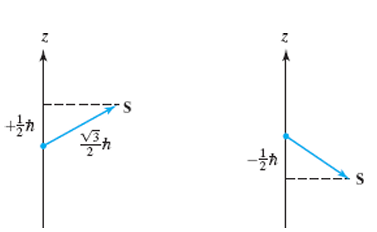
\includegraphics[width=0.4\textwidth]{Figures/10.1.png}
        \caption{
            \centering
            \parbox{\linewidth}{
                \centering 
                电子自旋矢量相对于 $z$ 轴的可能方向。在每种\\
                情况下,$\mathbf{S}$ 都位于以 $z$ 轴为轴的圆锥表面上。
            }
        }
        \label{fig:10.1}
    \end{figure}

    我们之前讨论过的波函数是粒子空间坐标的函数:$\psi = \psi\left(x,y,z\right)$。我们可能想问:自旋本征函数$\alpha$和$\beta$的变量是什么呢?有时,人们在谈论自旋坐标 $\omega$ 时,并没有明确说明这个坐标是什么。通常情况下,人们把自旋量子数 $m_s$ 作为自旋特征函数所依赖的变量。与空间波函数相比,这种程序很不寻常;但因为我们只有两种可能的电子自旋特征函数和本征值,所以这是一种方便的选择。我们有
    \begin{equation}
        \alpha = \alpha\left(m_s\right), \quad
        \beta = \beta\left(m_s\right)
        \label{eq:10.10}
    \end{equation}

    像往常一样,我们希望对本征函数进行归一化处理。单粒子空间波函数的三个变量范围在$-\infty$到$+\infty$之间连续变化,则归一化条件意味着
    \begin{equation*}
        \int_{-\infty}^{\infty} \int_{-\infty}^{\infty} \int_{-\infty}^{\infty} \left|\psi\left(x, y, z\right)\right|^2\: \mathrm{d}x\: \mathrm{d}y\: \mathrm{d}z = 1
    \end{equation*}
    电子自旋本征函数的变量 $m_s$ 只有 $+\frac{1}{2}$ 和 $-\frac{1}{2}$ 两个离散值。因此,对单粒子自旋本征函数的归一化意味着
    \begin{equation}
        \sum_{m_{s}=-1/2}^{1/2} \left|\alpha \left(m_{s}\right)\right|^{2} = 1, \quad \sum_{m_{s}=-1/2}^{1/2} \left|\beta \left(m_{s}\right)\right|^{2} = 1
        \label{eq:10.11}
    \end{equation}
    因为本征函数$\alpha$和$\beta$对应于厄米算符$\hat{S}_z$的不同本征值,所以它们是正交的:
    \begin{equation}
        \sum_{m_{s}=-1/2}^{1/2} \alpha^ * \left(m_{s}\right) \beta \left(m_{s}\right) = 0
        \label{eq:10.12}
    \end{equation}
    令$\alpha\left(m_s\right) = \delta_{m_s, 1/2}$,$\beta\left(m_s\right) = \delta_{m_s, -1/2}$,其中$\delta_{jk}$是Kronecker $\delta$函数,我们就满足了(\ref{eq:10.11})和(\ref{eq:10.12})。

    当我们考虑电子的完全波函数(包括空间和自旋变量)时,我们将根据以下公式对其进行归一化处理
    \begin{equation}
        \boxed{
            \sum_{m_s=-1/2}^{1/2} \int_{-\infty}^{\infty} \int_{-\infty}^{\infty} \int_{-\infty}^{\infty} \left|\psi\left(x, y, z, m_s\right)\right|^2 \:\mathrm{d}x \:\mathrm{d}y \:\mathrm{d}z = 1
        }
        \label{eq:10.13}
    \end{equation}
    符号
    \begin{equation*}
        \int \left|\psi\left(x, y, z, m_s\right)\right|^2 \:\mathrm{d}\tau
    \end{equation*}
    表示对自旋变量求和,对空间变量全范围积分,如 (\ref{eq:10.13}) 所示。符号 $\int \:\mathrm{d}v$ 表示对系统空间变量全范围的积分。

    \begin{quote}
        \small
        \noindent
        电子目前被认为是一种没有子结构的点状基本粒子。高能电子-正电子碰撞实验表明,没有证据表明电子的大小不为零,并将电子半径的上限为$3 \times 10^{-19} \:\mathrm{m}$[D. Bourilkov, \textit{Phys. Rev. D}, \textbf{62}, 076005 (2020); \url{arxiv.org/abs/hep-ph/0002172}.]。质子和中子是由夸克构成的,因此不是基本粒子。质子的均方根电荷半径为$0.88 \times 10^{-15} \:\mathrm{m}$。
    \end{quote}

\section{自旋和氢原子}
\label{sec:10.2 Spin and the Hydrogen Atom}

    具体说明电子状态的波函数不仅取决于$x$、$y$和$z$坐标,还取决于电子的自旋状态。这对氢原子的波函数和能级有什么影响?

    在很好的近似条件下,电子系统的哈密顿算符不涉及自旋变量,而只是空间坐标和关于空间坐标的导数的函数。因此,我们可以将单个电子的定态波函数分离为空间和自旋部分的乘积:
    \begin{equation*}
        \psi\left(x,y,z\right)g\left(m_s\right)
    \end{equation*}
    其中的$g\left(m_s\right)$是$\alpha$或$\beta$的其中之一,取决于$m_s = +\frac{1}{2}$或$m_s = -\frac{1}{2}$。[更一般地,$g\left(m_s\right)$可以是$\alpha$和$\beta$的线性组合;$g\left(m_s\right) = c_1 \alpha + c_2\beta$。]由于哈密顿算符对自旋波函数没有作用,我们有
    \begin{equation*}
        \hat{H} \left[\psi\left(x, y, z\right) g\left(m_s\right)\right] = g\left(m_s\right) \hat{H} \psi\left(x, y, z\right) = E \left[\psi\left(x, y, z\right) g\left(m_s\right)\right]
    \end{equation*}
    我们得到了与之前未考虑自旋时相同的能量。引入自旋唯一的不同是使得可能的状态数翻倍。与状态$\psi\left(x, y, z\right)$不同,我们有两个可能的状态$\psi\left(x, y, z\right) \alpha$和$\psi\left(x, y, z\right) \beta$。当我们考虑自旋时,氢原子能级的简并度是$2n^2$而不是$n^2$。

\section{自旋-统计定理}
\label{sec:10.3 Spin-Statistics Theorem}

    假设我们有一个由多个全同粒子组成的系统。在经典力学中,粒子的全同性不会导致特殊的后果。例如,考虑一下在台球桌上滚动的完全相同的台球。我们可以跟踪任何一个球的运动,比如通过拍摄系统的运动图像。我们可以说,一号球沿着某条轨迹运动,二号球沿着另一条确定的轨迹运动,以此类推,这些轨迹是由牛顿运动定律决定的。因此,虽然这些球是相同的,但我们可以通过指定每个球的运动轨迹来区分它们。球的特性对它们的运动没有特殊的影响。

    在量子力学中,不确定性原理告诉我们,我们无法追踪微观“粒子”的确切路径。如果系统中的微观粒子都具有不同的质量、电荷或自旋,我们就可以利用其中的一个特性来区分粒子。但如果它们都是相同的,那么我们在经典力学中区分它们的一种方法——即指定它们的路径——在量子力学中就会因为不确定性原理而丧失。因此,由相互作用的全同粒子组成的系统的波函数一定无法区分不同的粒子。例如,在第\ref{chap:9}章微扰理论处理氦原子激发态时,我们看见函数$1s\left(1\right)2s\left(2\right)$(说明电子1在$1s$轨道而电子2在$2s$轨道)不是一个正确的零级波函数。相反地,我们不得不使用函数$2^{-1/2}\left[1s\left(1\right)2s\left(2\right) \pm 1s\left(2\right)2s\left(1\right)\right]$,它无法指明电子在哪个轨道上。(如果相同的粒子彼此分离得很好,使它们的波函数不重叠,它们就可以被视为是可区分的。)

    现在,我们来推导量子力学中全同粒子的不可区分性对波函数的限制。由 $n$ 个相同微观粒子组成的系统的波函数取决于粒子的空间变量和自旋变量。对于粒子1,这些变量为$x_1$、$y_1$、$z_1$和$m_{s1}$。令$q_1$表示所有这四个变量。则$\psi = \psi\left(q_1, q_2, \ldots, q_n\right)$。

    我们定义交换两个粒子1和2所有坐标的算符$\hat{P}_{12}$为\textbf{交换算符}或\textbf{置换算符}(exchange or permutation operator):
    \begin{equation}
        \boxed{
            \hat{P}_{12} f\left(q_1, q_2, q_3, \ldots, q_n\right) = f\left(q_2, q_1, q_3, \ldots, q_n\right)
        }
        \label{eq:10.14}
    \end{equation}
    例如,对某表示电子1在$1s$轨道自旋向上而电子2在$3s$轨道自旋向下的函数,算符$\hat{P}_{12}$的作用为
    \begin{equation}
        \hat{P}_{12}\left[1s\left(1\right)\alpha\left(1\right)3s\left(2\right)\beta\left(2\right)\right] = 1s\left(2\right)\alpha\left(2\right)3s\left(1\right)\beta\left(1\right)
        \label{eq:10.15}
    \end{equation}

    $\hat{P}_{12}$的本征函数是什么?将$\hat{P}_{12}$作用两次,我们得到了原函数:
    \begin{equation*}
        \hat{P}_{12} \hat{P}_{12} f\left(q_1, q_2, \ldots, q_n\right) = \hat{P}_{12} f\left(q_2, q_1, \ldots, q_n\right) = f\left(q_1, q_2, ..., q_n\right)
    \end{equation*}
    因此,$\hat{P}_{12}^2 = \hat{1}$。设$\hat{P}_{12}$的本征函数和本征值分别为$w_i$和$c_i$。我们有$\hat{P}_{12} w_i = c_i w_i$。作用两次后,我们得到$\hat{P}_{12}^2 w_i = c_1 P_{12} w_i$。将$\hat{P}_{12}^2 = \hat{1}$和$\hat{P}_{12} w_i = c_i w_i$代入$\hat{P}_{12}^2 w_i = c_1 P_{12} w_i$,我们得到$w_i = c_i^2 w_i$。由于零不能作为本征函数,我们可以在两边同时除以$w_i$,得到$c_i^2 = 1$。因此,$c_i = \pm 1$。$\hat{P}_{12}$(以及任何平方为单位算符的线性算符)的本征值是$+1$和$-1$。

    若$w_+$是$\hat{P}_{12}$的本征函数,对应于本征值$+1$,则
    \begin{equation*}
        \hat{P}_{12}w_{+}\left(q_1, q_2, \ldots, q_n\right) = \left(+1\right)w_{+}\left(q_1, q_2, \ldots, q_n\right)
    \end{equation*}
    \begin{equation}
        \boxed{
            w_{+}\left(q_{2}, q_{1}, \ldots, q_{n}\right) = w_{+}\left(q_{1}, q_{2}, \ldots, q_{n}\right)
        }
        \label{eq:10.16}
    \end{equation}
    当粒子 1 和粒子 2 相互交换时,具有不变性质(\ref{eq:10.16})的函数(如 $w_+$)被称为与粒子 1 和粒子 2 相互交换\textbf{对称}(symmetric)的函数。对于本征值$-1$,我们有
    \begin{equation}
        \boxed{
            w_{-}\left(q_{2}, q_{1}, \ldots, q_{n}\right) = -w_{-}\left(q_{1}, q_{2}, \ldots, q_{n}\right)
        }
        \label{eq:10.17}
    \end{equation}
    (\ref{eq:10.17})的函数(如 $w_-$)被称为与粒子 1 和粒子 2 相互交换\textbf{反对称}(antisymmetric)的函数,这意味着将$w_-$乘以$-1$会得到交换后的函数。任意函数$f\left(q_1, q_2, \ldots, q_n\right)$对粒子1和2交换对称或是交换反对称无关紧要。

    不要混淆粒子互换的对称或非对称性质与空间反转的偶函数或奇函数性质。对于粒子1和2的交换,函数$x_1 + x_2$是交换对称的,它是$x_1$和$x_2$的奇函数。函数$x_1^2 + x_2^2$是交换对称的,但它是$x_1$和$x_2$的偶函数。

    算符$\hat{P}_{ik}$定义为
    \begin{equation}
        \hat{P}_{ik} f \left(q_1, \ldots, q_i, \ldots, q_k, \ldots, q_n\right) = f \left(q_1, \ldots, q_k, \ldots, q_i, \ldots, q_n\right)
        \label{eq:10.18}
    \end{equation}
    与$\hat{P}_{12}$类似,$\hat{P}_{ik}$的本征值为$+1$和$-1$。

    现在我们来看看由 $n$ 个相同的微观粒子组成的系统的波函数。由于粒子是无法区分的,我们给它们贴标签的方式不会影响系统的状态。因此,两个波函数
    \begin{equation*}
        \psi\left(q_1, \ldots, q_i, \ldots, q_k, \ldots, q_n\right) \quad \text{和} \quad \psi\left(q_1, \ldots, q_k, \ldots, q_i, \ldots, q_n\right)
    \end{equation*}
    必须对应于系统的相同状态。对应同一状态的两个波函数最多只能相差一个乘法常数。因此
    \begin{equation*}
        \begin{aligned}
            \psi\left(q_1, \ldots, q_k, \ldots, q_i, \ldots, q_n\right) &= c \psi\left(q_1, \ldots, q_i, \ldots, q_k, \ldots, q_n\right) \\
            \hat{P}_{ik} \psi\left(q_1, \ldots, q_i, \ldots, q_k, \ldots, q_n\right) &= c \psi\left(q_1, \ldots, q_i, \ldots, q_k, \ldots, q_n\right)
        \end{aligned}
    \end{equation*}
    最后一个方程表明$\psi$是算符$\hat{P}_{ik}$的本征函数。但是我们知道$\hat{P}_{ik}$的本征值只能是$+1$或$-1$。我们得出结论:由 $n$ 个全同粒子组成的系统,其波函数必须与任意两个全同粒子 $i$ 和 $k$ 的互换对称或反对称。由于 $n$ 个粒子都是相同的,我们不可能让波函数与某些互换对称,而与其他互换反对称。因此,$n$ 个完全相同的粒子的波函数必须要么与每一种可能的交换对称,要么与两个粒子的每一种可能的交换反对称。[刚才的论证并不严谨。完全相同的粒子系统的波函数对于两个粒子的互换必须是完全对称或完全反对称的说法称为\textit{对称化假设}(symmetrization postulate)。]

    我们已经看到,全同粒子系统的波函数有两种可能的情况,即对称和非对称情况。实验证据(如稍后讨论的元素周期表)表明,对于电子来说,只有反对称情况才会出现。因此,我们有了量子力学的另一个假设,即\textit{电子系统的波函数在任意两个电子互换时必须是反对称的}。

    1926 年,狄拉克根据理论研究和实验数据得出结论:电子要求反对称波函数,光子要求对称波函数。然而,狄拉克和其他物理学家在 1926 年错误地认为所有物质粒子都要求反对称波函数。1930 年,实验数据表明,$\alpha$ 粒子($s=0$)要求对称波函数;物理学家最终认识到,决定一个全同粒子系统要求对称波函数还是反对称波函数的是粒子的自旋性质。具有半整数自旋量子数($s = \frac{1}{2}, \frac{3}{2}$,等等)的粒子要求反对称波函数,而具有整数自旋量子数($s = 0, 1, 2$,等等)的粒子要求对称波函数。1940 年,物理学家沃尔夫冈·泡利(Wolfgang Pauli)利用相对论量子场论证明了这一结果。要求反对称波函数的粒子,如电子,被称为\textbf{费米子}(fermions)(以 E. Fermi 命名),而要求对称波函数的粒子,如离子,则被称为\textbf{玻色子}(bosons)(以 S. N. Bose 命名)。在非相对论量子力学中,我们必须假设,如果粒子具有半整数自旋量子数,则全同粒子系统的波函数在任意两个粒子互换时必须是反对称的;如果粒子具有整数自旋量子数,则波函数在互换时必须是对称的。这句话被称为\textbf{自旋-统计定理}(spin-statistics theorem)(因为玻色子系统的统计力学与费米子系统的统计力学不同)。

    自旋统计定理有许多不同有效性的证明;见 I. Duck and E. C. G. Sudurshan, \textit{Pauli and the Spin-Statistics Theorem}, World Scientific, 1997;\textit{Am. J. Phys.}, \textbf{66}, 284 (1998); Sudurshan and Duck, \textit{Pramana-J. Phys.}, \textbf{61}, 645 (2003) (见 \url{www.ias.ac.in/pramana/v61/p645/fulltext.pdf})。一些实验以极高的精度证实了自旋统计定理的有效性;见 G. M. Tino, \textit{Fortschr. Phys.}, \textbf{48}, 537 (2000) (可查阅 \url{arxiv.org/abs/quant-ph/9907028})。

    自旋-统计定理对完全相同的费米子系统有一个重要的影响。反对称要求意味着
    \begin{equation}
        \psi\left(q_1, q_2, q_3, \ldots, q_n\right) = -\psi\left(q_2, q_1, q_3, \ldots, q_n\right)
        \label{eq:10.19}
    \end{equation}
    考虑当电子1和2有相同坐标时$\psi$的值,即$x_1 = x_2$,$y_1 = y_2$,$z_1 = z_2$,$m_{s1} = m_{s2}$。在(\ref{eq:10.19})中令$q_2 = q_1$,我们得到
    \begin{equation*}
        \begin{aligned}
            \psi\left(q_1, q_1, q_3, \ldots, q_n\right) &= -\psi\left(q_1, q_1, q_3, \ldots, q_n\right) \\
            2\psi &= 0
        \end{aligned}
    \end{equation*}
    \begin{equation}
        \psi\left(q_1, q_1, q_3, \ldots, q_n\right) = 0
        \label{eq:10.20}
    \end{equation}
    因此,两个自旋相同的电子在三维空间的同一点出现的概率为零。(“自旋相同”意味着$m_s$值相等。)由于$\psi$是连续函数,方程(\ref{eq:10.20})说明在空间中发现两个自旋相同的电子彼此靠近的概率非常小。因此,反对称要求迫使自旋相同的电子彼此分开。为了描述这一点,人们常说这种电子之间存在\textbf{泡利斥力}(Pauli repulsion)。这种 “斥力”并不是一种真正的物理力,而是电子波函数在交换时必须是反对称的这一事实的反映。

    对称或反对称波函数的要求也适用于两个或多个全同复合粒子的系统。例如,考虑分子\ce{^16 O2}。\ce{^16 O}的核由8个质子和8个中子组成。每个质子和中子都满足$s = \frac{1}{2}$,都是费米子。因此,交换两个\ce{O}原子核相当于交换16个费米子的坐标,需要将分子的波函数乘以$\left(-1\right)^{16} = 1$。因此,分子\ce{^16 O2}的波函数在核坐标交换时是对称的。对相同原子核交换对称性或反对称性的要求会影响分子波函数的简并性,并导致转动配分函数中的对称数[见\textit{McQuarrie} (2000), pp. 104-105]。

    对于包含 $m$ 个全同玻色子和 $n$ 个全同费米子的两个相同复合粒子的交换,波函数需乘以$\left(+1\right)^m$\\$\left(-1\right)^n = \left(-1\right)^n$。

    因此,如果复合粒子包含奇数个费米子,那么它就是费米子,否则就是玻色子。

    当使用变分原理(第 \ref{sec:8.1 The Variation Theorem} 节)来获取原子和分子的近似电子波函数时,要求试探函数具有良好的稳定性,其中包括要求它具有反对称性。

\section{氦原子}
\label{sec:10.4 Th Helium Atom}

    现在,我们从电子自旋和反对称要求的角度重新考虑氦原子。在第\ref{sec:9.3 Perturbation Treatment of the Helium-Atom Ground State}节对氦原子进行微扰处理时,我们发现基态的零级波函数为$1s\left(1\right)1s\left(2\right)$。为了引入自旋,我们必须将该空间波函数与自旋本征函数相乘。因此,我们考虑两个电子可能的自旋本征函数。使用符号$\alpha\left(1\right)\alpha\left(2\right)$表示电子1和电子2的自旋向上状态,$\alpha\left(1\right)$代表了$\alpha\left(m_{s1}\right)$。因为每个电子都有两种可能的自旋状态,因此我们一眼就能看到四种可能的自旋函数:
    \begin{equation*}
        \alpha\left(1\right)\alpha\left(2\right), \quad \beta\left(1\right)\beta\left(2\right), \quad \alpha\left(1\right)\beta\left(2\right), \quad \alpha\left(2\right)\beta\left(1\right)
    \end{equation*}
    前两个函数没有任何问题,但第三和第四个函数违反了全同粒子不可区分的原则。例如,第三个函数表明电子1自旋向上而电子2自旋向下,这确实区分了电子1和2。更正式的说法是,如果我们将$\hat{P}_{12}$作用于这些函数,会发现前两个函数满足交换对称的要求,而后两个既不满足交换对称也不满足交换反对称,因此是不可接受的。

    现在怎么办?回想一下,我们在处理氦激发态时也遇到了基本相同的情况(第 \ref{sec:9.7 Perturbation Treatment of the First Excited State of Helium} 节),我们从函数$1s\left(1\right)2s\left(2\right)$和$2s\left(1\right)1s\left(2\right)$开始。我们发现这些区分了电子1和2的函数不是零级校正波函数,正确的零级校正波函数为$2^{-1/2}\left[1s\left(1\right)2s\left(2\right) \pm 2s\left(1\right)1s\left(2\right)\right]$。这一结果强烈表明,我们需要用下式来代替$\alpha\left(1\right)\beta\left(2\right)$和$\beta\left(1\right)\alpha\left(2\right)$:
    \begin{equation}
        2^{-1/2}\left[\alpha\left(1\right)\beta\left(2\right) \pm \beta\left(1\right)\alpha\left(2\right)\right]
        \label{eq:10.21}
    \end{equation}
    这些函数是$\alpha\left(1\right)\beta\left(2\right)$和$\beta\left(1\right)\alpha\left(2\right)$的归一化线性组合,也是$\hat{P}_{12}$的本征函数。它们是交换对称或反对称的。当电子1和电子2交换时,$2^{-1/2}\left[\alpha\left(1\right)\beta\left(2\right) + \beta\left(1\right)\alpha\left(2\right)\right]$变为了$2^{-1/2}\left[\alpha\left(2\right)\beta\left(1\right) + \beta\left(2\right)\right.$\\$\left.\alpha\left(1\right)\right]$,与原函数一致。相反地,$2^{-1/2}\left[\alpha\left(1\right)\beta\left(2\right) - \beta\left(1\right)\alpha\left(2\right)\right]$变为$-2^{-1/2}\left[\alpha\left(2\right)\beta\left(1\right) - \beta\left(2\right)\alpha\left(1\right)\right]$,等于$-1$与原函数相乘。为了证明(\ref{eq:10.21})是归一化的,我们有
    \begin{equation*}
        \begin{aligned}
            \sum_{m_{s1}} & \sum_{m_{s2}} \frac{1}{\sqrt{2}} \left[\alpha\left(1\right) \beta\left(2\right) \pm \beta\left(1\right) \alpha\left(2\right)\right]^* \frac{1}{\sqrt{2}} \left[\alpha\left(1\right) \beta\left(2\right) \pm \beta\left(1\right) \alpha\left(2\right)\right] \\
            & = \frac{1}{2} \sum_{m_{s1}} \left|\alpha\left(1\right)\right|^{2} \sum_{m_{s2}} \left|\beta\left(2\right)\right|^{2} \pm \frac{1}{2} \sum_{m_{s1}} \alpha^{*}\left(1\right) \beta\left(1\right) \sum_{m_{s2}} \beta^{*}\left(2\right) \alpha\left(2\right) \\
            & \pm \frac{1}{2} \sum_{m_{s1}} \beta^{*}\left(1\right)\alpha\left(1\right) \sum_{m_{s2}} \alpha^{*}\left(2\right)\beta\left(2\right) + \frac{1}{2} \sum_{m_{s1}} \left|\beta\left(1\right)\right|^{2} \sum_{m_{s2}} \left|\alpha\left(2\right)\right|^{2} = 1
        \end{aligned}
    \end{equation*}
    其中我们用到了正交关系(\ref{eq:10.11})和(\ref{eq:10.12})。

    因此,具有正确交换性质的四个归一化双电子自旋本征函数是
    \begin{empheq}[box=\fbox, left={\text{对称:}\empheqlbrace}]{align}
        &\alpha\left(1\right)\alpha\left(2\right) \label{eq:10.22}\\
        &\beta\left(1\right)\beta\left(2\right) \label{eq:10.23}\\
        &\left[\alpha\left(1\right)\beta\left(2\right) + \beta\left(1\right)\alpha\left(2\right)\right] / \sqrt{2} \label{eq:10.24}
    \end{empheq}
    \begin{equation}
        \boxed{
            \text{反对称:}\left[\alpha\left(1\right)\beta\left(2\right) - \beta\left(1\right)\alpha\left(2\right)\right] / \sqrt{2}
        }
        \label{eq:10.25}
    \end{equation}

    我们现在将自旋引入\ce{He}的基态零级校正波函数中。函数$1s\left(1\right)1s\left(2\right)$满足交换对称。包括自旋在内的完全电子波函数必须是交换反对称的。因此,我们必须将某个交换反对称的自旋波函数与交换对称的空间波函数$1s\left(1\right)1s\left(2\right)$相乘。只有一个反对称双电子自旋函数,因此氦原子的基态零阶波函数(包括自旋)为
    \begin{equation}
        \psi^{\left(0\right)} = 1s\left(1\right)1s\left(2\right) \cdot 2^{-1/2}\left[\alpha\left(1\right)\beta\left(2\right) - \beta\left(1\right)\alpha\left(2\right)\right]
        \label{eq:10.26}
    \end{equation}
    $\psi^{\left(0\right)}$是$\hat{P}_{12}$的本征函数,对应于本征值$-1$。

    在很好的近似条件下,哈密顿量不包含自旋项,因此在基态波函数中引入自旋因子不会影响能量。而且,当考虑自旋时,氦的基态仍然是非简并的。

    为了进一步证明自旋因子并不影响能量,我们假设正在使用试探函数$\phi = f\left(r_1, r_2, r_{12}\right)2^{-1/2}$\\$ \left[\alpha\left(1\right)\beta\left(2\right) - \beta\left(1\right)\alpha\left(2\right)\right]$对 \ce{He} 的基态进行变分计算,其中$f$是满足两电子坐标交换对称的归一化函数。变分积分为
    \begin{equation*}
        \begin{aligned}
            \int \phi^* \hat{H} \phi \: \mathrm{d}\tau =& \sum_{m_{s1}} \sum_{m_{s2}} \int \int f^* \left(r_1, r_2, r_{12}\right) \frac{1}{\sqrt{2}} \left[\alpha\left(1\right)\beta\left(2\right) - \beta\left(1\right)\alpha\left(2\right)\right]^* \\
            & \times \hat{H} f \left(r_1, r_2, r_{12}\right) \frac{1}{\sqrt{2}} \left[\alpha\left(1\right)\beta\left(2\right) - \beta\left(1\right)\alpha\left(2\right)\right] \: \mathrm{d}v_1 \: \mathrm{d}v_2
        \end{aligned}
    \end{equation*}
    因为$\hat{H}$对自旋波函数没有作用,所以变分积分变为
    \begin{equation*}
        \int \int f^* \hat{H} f \:\mathrm{d} v_1 \: \mathrm{d} v_2 \sum_{m_{s1}} \sum_{m_{s2}} \frac{1}{2} \left[\alpha\left(1\right)\beta\left(2\right) - \beta\left(1\right)\alpha\left(2\right)\right]^2
    \end{equation*}
    又因为自旋函数(\ref{eq:10.25})是归一化的,所以变分积分简化为$\int \int f^* \hat{H} f \:\mathrm{d} v_1 \: \mathrm{d} v_2$,这就是我们引入自旋之前的变分积分。

    现在,我们来考虑\ce{He}的激发态。我们知道,最低激发态的零级空间波函数为$2^{-1/2}\left[1s\left(1\right)2s\left(2\right) \right.$\\$\left. - 2s\left(1\right)1s\left(2\right)\right]$[式(\ref{eq:9.103})]。因为空间函数是交换反对称的,我们必须乘上一个交换对称的自旋函数。我们可以使用三个交换对称的双电子自旋函数中的任意一个,因此我们得到的不是之前发现的非简并能级,而是一个具有三个零级波函数的三重简并能级
    \begin{equation}
        2^{-1/2}\left[1s\left(1\right)2s\left(2\right) - 2s\left(1\right)1s\left(2\right)\right]\alpha\left(1\right)\alpha\left(2\right)
        \label{eq:10.27}
    \end{equation}
    \begin{equation}
        2^{-1/2}\left[1s\left(1\right)2s\left(2\right) - 2s\left(1\right)1s\left(2\right)\right]\beta\left(1\right)\beta\left(2\right)
        \label{eq:10.28}
    \end{equation}
    \begin{equation}
        2^{-1/2}\left[1s\left(1\right)2s\left(2\right) - 2s\left(1\right)1s\left(2\right)\right]2^{-1/2}\left[\alpha\left(1\right)\beta\left(2\right) + \beta\left(1\right)\alpha\left(2\right)\right]
        \label{eq:10.29}
    \end{equation}
    对于下一个激发态,由于要求完全波函数具有交换反对称性,因此会产生零阶波函数
    \begin{equation}
        2^{-1/2}\left[1s\left(1\right)2s\left(2\right) + 2s\left(1\right)1s\left(2\right)\right]2^{-1/2}\left[\alpha\left(1\right)\beta\left(2\right) - \beta\left(1\right)\alpha\left(2\right)\right]
        \label{eq:10.30}
    \end{equation}
    同样的考虑也适用于 $1s2p$ 状态。

\section{泡利不相容原理}
\label{sec:10.5 The Pauli Exclusion Principle}

    到目前为止,我们还没有看到电子自旋和不对称要求带来任何非常惊人的后果。在氢原子和氦原子中,波函数中的自旋因子和不对称性要求只是影响了能级的简并性,而不会(除了稍后要考虑的非常小的影响)影响之前得到的能量。锂的情况则完全不同。

    假设我们把锂原子中的电子间斥力看作是对哈密顿其余项的微扰。按照处理氦的相同步骤,未扰动波函数是三个类氢函数的乘积。对于基态
    \begin{equation}
        \psi^{\left(0\right)} = 1s\left(1\right)1s\left(2\right)1s\left(3\right)
        \label{eq:10.31}
    \end{equation}
    零级(未扰动)能量为[方程(\ref{eq:9.48})及(\ref{eq:9.50})之后的段落]
    \begin{equation*}
        E^{\left(0\right)} = -\left(\frac{1}{1^2} + \frac{1}{2^2} + \frac{1}{1^2}\right)\left(\frac{Z^2\mathrm{e}^2}{8\pi \varepsilon_0a_0}\right) = -27 \left(\frac{\mathrm{e}^2}{8\pi \varepsilon_0a_0}\right) = -27  \left(13.606 \: \mathrm{eV}\right) = -367.4 \: \mathrm{eV}
    \end{equation*}

    能量的一级校正为$E^{\left(1\right)} = \left\langle \psi^{\left(0\right)} \middle| \hat{H}' \middle| \psi^{\left(0\right)} \right\rangle$,其中微扰项$\hat{H}'$包含了电子间斥力,则
    \begin{equation*}
        \begin{aligned}
            E^{\left(1\right)} = \int \left|1s\left(1\right)\right|^2 \left|1s\left(2\right)\right|^2 \left|1s\left(3\right)\right|^2 \frac{\mathrm{e}^2}{4\pi\varepsilon_0 r_{12}} \:\mathrm{d}v &+ \int \left|1s\left(1\right)\right|^2 \left|1s\left(2\right)\right|^2 \left|1s\left(3\right)\right|^2 \frac{\mathrm{e}^2}{4\pi\varepsilon_0 r_{23}} \:\mathrm{d}v \\
            &+ \int \left|1s\left(1\right)\right|^2 \left|1s\left(2\right)\right|^2 \left|1s\left(3\right)\right|^2 \frac{\mathrm{e}^2}{4\pi\varepsilon_0 r_{13}} \:\mathrm{d}v
        \end{aligned}
    \end{equation*}
    在这些定积分中,我们给虚拟积分变量贴标签的方式不会影响它们的值。如果我们互换第二个积分中变量的标号 1 和 3,它就会转换成第一个积分。因此,这两个积分相等。将第三个积分中的标号 2 和 3 互换后,它也等于第一个积分。因此
    \begin{equation*}
        E^{\left(1\right)} = 3 \int \int \left|1s\left(1\right)\right|^2 \left|1s\left(2\right)\right|^2 \frac{\mathrm{e}^2}{4\pi \varepsilon_0 r_{12}} \:\mathrm{d}v_1\: \mathrm{d}v_2 \int \left|1s\left(3\right)\right|^2 \:\mathrm{d}v_3
    \end{equation*}
    对电子3积分的值为1(归一化)。电子 1 和电子 2 的积分是在氦的微扰处理中计算得到的,以及[式(\ref{eq:9.52})和(\ref{eq:9.53})]
    \begin{equation*}
        E^{\left(1\right)} = 3\left(\frac{5Z}{4}\right)\left(\frac{\mathrm{e}^2}{8\pi \varepsilon_0a_0}\right) = \frac{45}{4} \left(13.606 \: \mathrm{eV}\right) = 153.1 \: \mathrm{eV}
    \end{equation*}
    \begin{equation*}
        E^{\left(0\right)} + E^{\left(1\right)} = -214.3 \: \mathrm{eV}
    \end{equation*}

    因为我们可以把零级扰动波函数作为试探函数(回顾第 \ref{sec:9.4 Variational Treatments of the Ground State of Helium} 节开头的讨论),根据变分原理,$E^{\left(0\right)} + E^{\left(1\right)}$等于或大于真实基态能量。锂基态能量的实验值通过将第一、第二和第三电离能相加得到,即[C. E. Moore, “Ionization Potentials and Ionization Limits,” publication NSRDS-NBS 34 of the National Bureau of Standards (1970); available at \url{www.nist.gov/data/nsrds/NSRDSNBS34.pdf}]
    \begin{equation*}
        -\left(5.39 + 75.64 + 122.45\right) \: \mathrm{eV} = -203.5 \: \mathrm{eV}
    \end{equation*}
    因此,此时我们的$E^{\left(0\right)} + E^{\left(1\right)}$比基态能量真实值低,这违反了变分原理。例外,假设的锂原子基态组态$1s^3$与第一电离势的低值和所有化学证据不符。如果我们继续这样做,原子序数为 $Z$ 的元素就会出现 $1s^Z$ 基态构型。我们不会得到众所周知的元素周期性行为。

    当然,我们的错误在于没有考虑自旋和反对称要求。假设的零级波函数$1s\left(1\right)1s\left(2\right)1s\left(3\right)$对于任意两个电子的互换是对称的。如果我们要有一个反对称函数$\psi^{\left(0\right)}$,我们必须将该空间交换对称函数与一个交换反对称自旋函数相乘。为三个电子构建完全对称的自旋函数非常容易,例如$\alpha\left(1\right)\alpha\left(2\right)\alpha\left(3\right)$。然而,要为三个电子构建一个完全反对称的自旋函数是不可能的。

    让我们考虑一下如何系统地构建三个电子的反对称函数。我们将使用 $f$、$g$ 和 $h$ 来表示电子坐标的三个函数,但并不指明我们考虑的是空间坐标还是自旋坐标,抑或两者兼而有之。我们从以下函数开始:
    \begin{equation}
        f\left(1\right)g\left(2\right)h\left(3\right)
        \label{eq:10.32}
    \end{equation}
    这显然不满足交换反对称。我们想要的反对称函数必须通过每一个置换算符$\hat{P}_{12}$、$\hat{P}_{13}$和$\hat{P}_{23}$转换成它的负值。将每个算符轮流作用到$f\left(1\right)g\left(2\right)h\left(3\right)$上,我们得到
    \begin{equation}
        f\left(2\right)g\left(1\right)h\left(3\right), \quad f\left(3\right)g\left(2\right)h\left(1\right), \quad f\left(1\right)g\left(3\right)h\left(2\right)
        \label{eq:10.33}
    \end{equation}
    我们可以尝试将反对称函数构造成四个函数 (\ref{eq:10.32}) 和 (\ref{eq:10.33}) 的线性组合,但这一尝试会失败。将$\hat{P}_{12}$作用于(\ref{eq:10.33})中的后两个函数,得到
    \begin{equation}
        f\left(3\right)g\left(1\right)h\left(2\right) \quad \text{和} \quad f\left(2\right)g\left(3\right)h\left(1\right)
        \label{eq:10.34}
    \end{equation}
    它不在(\ref{eq:10.32})和(\ref{eq:10.33})中。因此,我们必须将所有六个函数 (\ref{eq:10.32}) 至 (\ref{eq:10.34}) 纳入所需的反对称线性组合中。这六个函数是三个电子在 $f$、$g$ 和 $h$ 三个函数中的六$\left(3 \cdot 2 \cdot 1\right)$种可能排列。若$f\left(1\right)g\left(2\right)h\left(3\right)$是薛定谔方程的解,本征值为$E$,那么由于粒子的特性,(\ref{eq:10.32}) 至 (\ref{eq:10.34}) 的每个函数都是薛定谔方程的解,本征值相同(交换简并),以及这些函数的任意线性组合也是本征值为$E$的本征函数。

    反对称线性组合应具有如下形式:
    \begin{equation}
        \begin{aligned}
            c_1 f\left(1\right)g\left(2\right)h\left(3\right) + c_2 f\left(2\right)g\left(1\right)h\left(3\right) &+ c_3 f\left(3\right)g\left(2\right)h\left(1\right) + c_4 f\left(1\right)g\left(3\right)h\left(2\right) \\
            &+ c_5 f\left(3\right)g\left(1\right)h\left(2\right) + c_6 f\left(2\right)g\left(3\right)h\left(1\right)
        \end{aligned}
        \label{eq:10.35}
    \end{equation}
    因为$f\left(2\right)g\left(1\right)h\left(3\right) = \hat{P}_{12} f\left(1\right)g\left(2\right)h\left(3\right)$,为了使得(\ref{eq:10.35})成为$\hat{P}_{12}$的本征值为$-1$的本征函数,我们必须有$c_2 = -c_1$。同样地,$f\left(3\right)g\left(2\right)h\left(1\right) = \hat{P}_{13} f\left(1\right)g\left(2\right)h\left(3\right)$以及$f\left(1\right)g\left(3\right)h\left(2\right) = \hat{P}_{23} f\left(1\right)g\left(2\right)h\left(3\right)$,因此$c_3 = -c_1$和$c_4 = -c_1$。又因为$f\left(3\right)g\left(1\right)h\left(2\right) = \hat{P}_{12} f\left(1\right)g\left(3\right)h\left(2\right)$,我们必须有$c_5 = -c_3 = c_1$。同样地,有$c_6 = c_1$。因此,我们得出了线性组合
    \begin{equation}
        \begin{aligned}
            c_1 \left[ f\left(1\right)g\left(2\right)h\left(3\right) - f\left(2\right)g\left(1\right)h\left(3\right) - f\left(3\right)g\left(2\right)h\left(1\right) - f\left(1\right)g\left(3\right)h\left(2\right) \right. \\
            \left. + f\left(3\right)g\left(1\right)h\left(2\right) + f\left(2\right)g\left(3\right)h\left(1\right) \right]
        \end{aligned}
        \label{eq:10.36}
    \end{equation}
    容易证明,上式在交换$1-2$、$1-3$或$2-3$时都满足交换反对称。[将(\ref{eq:10.36})中的所有符号都变为$+$号,我们将得到一个完全对称的函数。]

    假设$f$、$g$和$h$互相正交,选择$c_1$的合适值使得(\ref{eq:10.36})归一化。将(\ref{eq:10.36})与其复共轭相乘,我们得到了很多项,但由于假设的正交性,涉及 (\ref{eq:10.36}) 中两个不同项的所有乘积的积分都消失了。例如,
    \begin{equation*}
        \begin{aligned}
            \int \left[f\left(1\right)g\left(2\right)h\left(3\right)\right]^*&f\left(2\right)g\left(1\right)h\left(3\right) \:\mathrm{d}\tau \\
            &= \int f^*\left(1\right)g\left(1\right)\:\mathrm{d}\tau_1 \int g^*\left(2\right)f\left(2\right)\:\mathrm{d}\tau_2 \int h^*\left(3\right)h\left(3\right)\:\mathrm{d}\tau_3 = 0 \cdot 0 \cdot 1 = 0
        \end{aligned}
    \end{equation*}
    由于 $f$、$g$和$h$已归一化,因此涉及 (\ref{eq:10.36}) 项与其自身复共轭的乘积的积分等于 1。因此,
    \begin{equation*}
        1 = \int \left|10.36\right|^2 \:\mathrm{d}\tau = \left|c_1\right|^2 \left(1+1+1+1+1+1\right)
    \end{equation*}
    \begin{equation*}
        c_1 = 1 / \sqrt{6}
    \end{equation*}
    我们可以按原样处理 (\ref{eq:10.36}),但如果我们将其视为以下三阶行列式的展开式 [式 (\ref{eq:8.24}) ],则最容易发现其性质:
    \begin{equation}
        \boxed{ 
            \frac{1}{\sqrt{6}}\begin{vmatrix}
                f\left(1\right) & g\left(1\right) & h\left(1\right) \\
                f\left(2\right) & g\left(2\right) & h\left(2\right) \\
                f\left(3\right) & g\left(3\right) & h\left(3\right)
            \end{vmatrix}
        }
        \label{eq:10.37}
    \end{equation}
    (另见问题8.22)。反对称性质在 (\ref{eq:10.37}) 中成立,因为交换两个电子相当于交换行列式的两行,行列式乘以$-1$。

    现在我们利用(\ref{eq:10.37})来证明不可能为三个电子构建一个反对称自旋函数。函数$f$、$g$和$h$可能是$\alpha$或$\beta$。若我们取$f = \alpha$、$g = \beta$和$h = \alpha$,则(\ref{eq:10.37})变为
    \begin{equation}
        \frac{1}{\sqrt{6}}\begin{vmatrix}
            \alpha\left(1\right) & \beta\left(1\right) & \alpha\left(1\right) \\
            \alpha\left(2\right) & \beta\left(2\right) & \alpha\left(2\right) \\
            \alpha\left(3\right) & \beta\left(3\right) & \alpha\left(3\right)
        \end{vmatrix}
        \label{eq:10.38}
    \end{equation}
    虽然(\ref{eq:10.38})是一个反对称函数,但它的值为零,我们必须舍去它。行列式的第一列和第三列相同,所以(第\ref{sec:8.3 Determinants}节)行列式的值为零。无论我们怎么取$f$、$g$和$h$,行列式至少有两列是相同的,所以我们无法构建一个非零的三电子交换反对称自旋函数。

    现在我们利用(\ref{eq:10.37})来构建锂的零级基态波函数,包括空间和自旋变量。函数 $f$、$g$ 和 $h$ 将同时涉及空间变量和自旋变量。我们选择
    \begin{equation}
        f\left(1\right) = 1s\left(1\right)\alpha\left(1\right)
        \label{eq:10.39}
    \end{equation}
    我们称具有(\ref{eq:10.39})形式的函数\textbf{自旋轨道}(spin-orbital)。\textit{自旋轨道是单电子空间轨道和单电子自旋函数的乘积。}

    若我们取$g\left(1\right) = 1s\left(1\right)\alpha\left(1\right)$,这使得(\ref{eq:10.37})的第一列和第二列相同,因此行列式的值为零。这是\textbf{泡利不相容原理}(Pauli Exclusion Principle)的一个特例:\textit{两个电子不能占据同一个自旋轨道。}另一种说法是,原子中不可能有两个电子的所有量子数具有相同的值。泡利不相容原理是由相同的自旋$-\frac{1}{2}$ 粒子组成的系统的波函数的更一般的反对称要求的结果,它不如反对称声明令人满意,因为不相容原理是基于近似(零阶)波函数的。

    因此,我们取$g\left(1\right) = 1s\left(1\right)\beta\left(1\right)$,从而使得$1s$轨道中的两个电子自旋相反。对于自旋轨道$h$,我们既不能取$1s\left(1\right)\alpha\left(1\right)$,也不能取$1s\left(1\right)\beta\left(1\right)$,因为这些选择会使行列式的值为零。我们取$h\left(1\right) = 2s\left(1\right)\alpha\left(1\right)$,从而得到了熟悉的\ce{Li}基态组态$1s^22s$,零级波函数为
    \begin{equation}
        \psi^{\left(0\right)} = \frac{1}{\sqrt{6}}\begin{vmatrix}
            1s\left(1\right)\alpha\left(1\right) & 1s\left(1\right)\beta\left(1\right) & 2s\left(1\right)\alpha\left(1\right) \\
            1s\left(2\right)\alpha\left(2\right) & 1s\left(2\right)\beta\left(2\right) & 2s\left(2\right)\alpha\left(2\right) \\
            1s\left(3\right)\alpha\left(3\right) & 1s\left(3\right)\beta\left(3\right) & 2s\left(3\right)\alpha\left(3\right)
        \end{vmatrix}
        \label{eq:10.40}
    \end{equation}
    特别要注意的是,(\ref{eq:10.40}) 并不是简单的空间和自旋部分的乘积(就像我们发现的 \ce{H} 和 \ce{He} 一样),而是多个项的线性组合,每个项都是空间和自旋部分的乘积。

    同样地,我们也可以取$h\left(1\right) = 2s\left(1\right)\beta\left(1\right)$,那么与氢一样,锂的基态是二重简并的,对应于 $2s$ 电子自旋的两种可能方向。我们可以使用轨道图来表明这点:
    \begin{equation*}
        \begin{matrix}
            1s & 2s \\
            \underline{\uparrow \downarrow} & \underline{\uparrow}
        \end{matrix} \qquad \text{和} \qquad \begin{matrix}
            1s & 2s \\
            \underline{\uparrow \downarrow} & \underline{\downarrow}
        \end{matrix}
    \end{equation*}
    每个空间轨道,例如$1s$或$2p_0$,可以容纳两个自旋相反的电子。一个自旋轨道,例如$2s\alpha$,只能容纳一个电子。

    虽说组态$1s^22p$与$1s^22s$具有相同的未扰动能量$E^{\left(0\right)}$,但当我们在计算$E^{\left(1\right)}$以及更高级的校正时引入了电子斥力,就会发现 $1s^22s$ 组态的能量较低,原因与氦的情况相同。

    考虑一下关于泡利不相容原理的一些观点,我们重述如下:\textit{在一个由相同费米子组成的系统中,没有两个粒子可以占据相同的状态。}如果我们有一个由 $n$ 个相互作用粒子组成的系统(例如原子),那么整个系统只有一个波函数(涉及 $4n$ 个变量)。由于粒子间的相互作用,波函数不能写成单个粒子波函数的乘积。因此,严格来说,我们不能谈论单个粒子的状态,只能谈论整个系统的状态。不过,如果粒子之间的相互作用不太大,那么作为初始近似,我们可以忽略它们,将系统的零阶波函数写成单个粒子波函数的乘积。在这个零阶波函数中,没有两个费米子的波函数(状态)是相同的。

    由于玻色子要求一个交换对称波函数,因此对给定状态下的玻色子数量没有限制。

    1925 年,爱因斯坦证明,在非相互作用玻色子的理想气体中,存在一个非常低的温度 $T_c$(称为凝结温度),高于这个温度时,基态玻色子的分数$f$可以忽略不计,但低于这个温度时,$f$ 会变得可观,并随着绝对温度 $T$ 变为 0 而变为 1。立方体中非相互作用玻色子的$f$满足的方程为$f = 1 - \left(T/T_c\right)^{3/2}, \: T < T_c$[\textit{McQuarrie} (2000), Section 10-4]。大量玻色子落入基态的现象被称为\textit{玻色-爱因斯坦凝聚}(Bose-Einstein condensation)。玻色-爱因斯坦凝聚对于确定超流体液体(其原子是玻色子)的性质非常重要,但液体\ce{He}中的原子间相互作用使理论分析变得困难。

    1995 年,物理学家成功地在气体中产生了玻色-爱因斯坦凝聚[\textit{Physics Today}, August 1995, p. 17; C. E. Wieman, \textit{Am. J. Phys.}, \textbf{64}, 847 (1996)]。他们使用了\ce{^37_87Rb}原子的气体。一个\ce{Rb}原子含有87个核子和37个电子,由于它具有偶数(124)个费米子,因此是玻色子。在激光、外加不均匀磁场和外加射频辐射的共同作用下,样品中的$10^4$ \ce{^87Rb}原子被冷却到$10^{-7} \: \mathrm{K}$,从而使相当一部分原子凝结成基态。然后,利用射频辐射去除大部分处于激发态的原子,留下由 2000 个原子组成的凝聚态,其中几乎所有原子都处于基态。实验中的每个\ce{Rb}都受到原子总自旋磁矩与外加磁场相互作用产生的势能函数$V\left(x,y,z\right)$的影响(第 \ref{sec:6.8 Zeeman effect} 节和第 \ref{sec:10.9 Spin Magnetic Moment} 节)。不均匀的外加磁场使得势能 $V$ 为三维谐振子(见问题4.20)的势能加上一个常数。玻色-爱因斯坦凝聚态中的\ce{Rb}原子处于这个谐振子势能的基态。

\section{斯莱特行列式}
\label{sec:10.6 Slater Determinants}

    斯莱特(Slater)在 1929 年指出,形式为 (\ref{eq:10.40}) 的行列式满足多电子原子的反对称要求。类似 (\ref{eq:10.40}) 的行列式称为\textbf{斯莱特行列式}(Slater Determinants)。斯莱特行列式的某一列中的所有元素都涉及相同的自旋轨道,而同一行中的所有元素都涉及相同的电子。(由于交换行列并不影响行列式的值,我们可以用另一种等价形式来书写斯莱特行列式)。

    考虑一下我们之前导出的零级氦波函数如何写成斯莱特行列式。对于基态组态$1s^2$,我们有自旋轨道$1s\alpha$和$1s\beta$。因此,斯莱特行列式为
    \begin{equation}
        \frac{1}{\sqrt{2}}\begin{vmatrix}
            1s\left(1\right)\alpha\left(1\right) & 1s\left(1\right)\beta\left(1\right) \\
            1s\left(2\right)\alpha\left(2\right) & 1s\left(2\right)\beta\left(2\right)
        \end{vmatrix} = 1s\left(1\right)1s\left(2\right) \frac{1}{\sqrt{2}}\left[\alpha\left(1\right)\beta\left(2\right) - \beta\left(1\right)\alpha\left(2\right)\right]
        \label{eq:10.41}
    \end{equation}
    与(\ref{eq:10.26})一致。对于与激发构型 $1s2s$ 相对应的态,我们有以下可能的自旋轨道$1s\alpha$、$1s\beta$、$2s\alpha$和$2s\beta$。因此,斯莱特行列式为
    \begin{equation*}
        \begin{aligned}
            D_1 &= \frac{1}{\sqrt{2}}\begin{vmatrix}
                1s\left(1\right)\alpha\left(1\right) & 2s\left(1\right)\alpha\left(1\right) \\
                1s\left(2\right)\alpha\left(2\right) & 2s\left(2\right)\alpha\left(2\right)
            \end{vmatrix}  \quad D_2 = \frac{1}{\sqrt{2}}\begin{vmatrix}
                1s\left(1\right)\alpha\left(1\right) & 2s\left(1\right)\beta\left(1\right) \\
                1s\left(2\right)\alpha\left(2\right) & 2s\left(2\right)\beta\left(2\right)
            \end{vmatrix} \\
            D_3 &= \frac{1}{\sqrt{2}}\begin{vmatrix}
                1s\left(1\right)\beta\left(1\right) & 2s\left(1\right)\alpha\left(1\right) \\
                1s\left(2\right)\beta\left(2\right) & 2s\left(2\right)\alpha\left(2\right)
            \end{vmatrix} \quad D_4 = \frac{1}{\sqrt{2}}\begin{vmatrix}
                1s\left(1\right)\beta\left(1\right) & 2s\left(1\right)\beta\left(1\right) \\
                1s\left(2\right)\beta\left(2\right) & 2s\left(2\right)\beta\left(2\right)
            \end{vmatrix}
        \end{aligned}
    \end{equation*}
    与 (\ref{eq:10.27}) 至 (\ref{eq:10.30}) 的比较表明,$1s2s$ 零阶波函数与这四个斯莱特行列式的关系如下:
    \begin{equation}
        2^{-1/2} \left[1s\left(1\right)2s\left(2\right) - 2s\left(1\right)1s\left(2\right)\right]\alpha\left(1\right)\alpha\left(2\right) = D_1
        \label{eq:10.42}
    \end{equation}
    \begin{equation}
        2^{-1/2} \left[1s\left(1\right)2s\left(2\right) - 2s\left(1\right)1s\left(2\right)\right]\beta\left(1\right)\beta\left(2\right) = D_4
        \label{eq:10.43}
    \end{equation}
    \begin{equation}
        2^{-1/2} \left[1s\left(1\right)2s\left(2\right) - 2s\left(1\right)1s\left(2\right)\right]2^{-1/2} \left[\alpha\left(1\right)\beta\left(2\right) + \beta\left(1\right)\alpha\left(2\right)\right] = 2^{-1/2} \left(D_2 + D_3\right)
        \label{eq:10.44}
    \end{equation}
    \begin{equation}
        2^{-1/2} \left[1s\left(1\right)2s\left(2\right) + 2s\left(1\right)1s\left(2\right)\right]2^{-1/2} \left[\alpha\left(1\right)\beta\left(2\right) - \beta\left(1\right)\alpha\left(2\right)\right] = 2^{-1/2} \left(D_2 - D_3\right)
        \label{eq:10.45}
    \end{equation}
    (要得到一个自旋和轨道角动量算子的特征函数的零级函数,我们有时必须对组态的斯莱特行列式进行线性组合;见第 \ref{chap:11} 章。)

    接下来,我们来看看斯莱特行列式的一些符号。与用$\alpha$和$\beta$表示自旋函数不同,人们通常在空间函数上加一横杠,表示自旋函数 $\beta$,而没有横杠的空间函数则表示自旋因子 $\alpha$。根据这种符号,(\ref{eq:10.40})可以写成
    \begin{equation}
        \psi^{\left(0\right)} = \frac{1}{\sqrt{6}}\begin{vmatrix}
            1s\left(1\right) & \overline{1s}\left(1\right) & 2s\left(1\right) \\
            1s\left(2\right) & \overline{1s}\left(2\right) & 2s\left(2\right) \\
            1s\left(3\right) & \overline{1s}\left(3\right) & 2s\left(3\right)
        \end{vmatrix}
        \label{eq:10.46}
    \end{equation}
    有了电子占据的自旋轨道,我们就可以很容易地构建斯莱特行列式。因此,斯莱特行列式通常使用简记符号,只需指定自旋轨道即可。在这种符号中,(\ref{eq:10.46}) 通常写为
    \begin{equation}
        \boxed{
            \psi^{\left(0\right)} = \left|1s \overline{1s}2s\right|
        }
        \label{eq:10.47}
    \end{equation}
    其中竖线表示行列式并乘以 $1/\sqrt{6}$。

    我们已经证明,因子 $1/\sqrt{6}$ 使由正交函数构成的三阶斯莱特行列式归一化。$n$阶行列式的展开式有$n!$项(问题8.20)。对于由正交轨道构成的$n$阶斯莱特行列式,与三阶行列式相同的推理表明:归一化常数为$1/\sqrt{n!}$。因此,在定义$n$阶斯莱特行列式时,我们总是加上因子$1/\sqrt{n!}$。

\section{微扰理论处理基态锂原子}
\label{sec:10.7 Perturbation Treatment of the Lithium Ground State}


















\section{变分法处理基态锂原子}
\label{sec:10.8 Variation Treatments of the Lithium Ground State}

\section{自旋磁矩}
\label{sec:10.9 Spin Magnetic Moment}

\section{电子自旋的梯度算符}
\label{sec:10.10 Ladder Operators for Electron Spin}

\section*{总结}

\section*{习题}
	
	% ===== CHAPTER 11 =====
\chapter{多电子原子}
\label{chap:11}
\section{Hartree-Fock自洽场方法}
\label{sec:11.1 The Hartree-Fock Self-Consistent-Field Method}

    对于氢原子,其精确波函数是已知的。对于氦和锂,通过在变分函数中引入电子间距离,已经计算出了非常精确的波函数。对于原子序数较高的原子,找到精确波函数的一种方法是首先使用Hartree–Fock方法找到一个近似波函数,我们将在本节中概述该方法。Hartree-Fock方法是多电子系统中使用原子和分子轨道的基础。

    $n$电子原子的哈密顿算符为
    \begin{equation}
        \hat{H} = -\frac{\hbar^2}{2m_{\mathrm{e}}} \sum_{i=1}^{n} \nabla_i^2 - \sum_{i=1}^{n} \frac{Z \mathrm{e}^2}{4\pi\varepsilon_0 r_i} + \sum_{i=1}^{n-1} \sum_{j=i+1}^{n} \frac{\mathrm{e}^2}{4\pi\varepsilon_0 r_{ij}}
        \label{eq:11.1}
    \end{equation}
    其中假设存在一个质量无限大的点状原子核(第\ref{sec:6.6 The Bound-State Hydrogen-Atom Wave Functions}节)。(\ref{eq:11.1})中的第一个求和包含了$n$个电子的动能算符。第二个求和为电子和核电荷$Z\mathrm{e}$之间的吸引势(\ref{eq:6.58})。对于中性原子,有$Z=n$。最后一个求和为电子排斥势。限制$j > i$避免了重复计算电子间排斥力,且舍去了如$\mathrm{e}^2/4\pi\varepsilon_0 r_{ii}$这样的项。哈密顿算符(\ref{eq:11.1})是不完整的,因为它忽略了自旋轨道和其他相互作用。略去的项较小(除了具有高$Z$值的原子,它们将在第\ref{sec:11.6 Spin-Orbit Interaction}和\ref{sec:11.7 The Atomic Hamiltonian}节中讨论。

\subsection*{Hartree自洽场方法}

    由于电子间排斥项$\mathrm{e}^2 / 4\pi\varepsilon_0r_{ij}$的存在,单原子的薛定谔方程无法分离变量。回忆处理氦原子的微扰法(第\ref{sec:9.3 Perturbation Treatment of the Helium-Atom Ground State}节),通过忽略这些排斥项,我们可以得到零级波函数。那么薛定谔方程就可以分离成$n$个单电子类氢方程。零级波函数就是$n$个类氢(单电子)轨道的乘积:
    \begin{equation}
        \psi^{(0)} = f_1(r_1, \theta_1, \phi_1) f_2(r_2, \theta_2, \phi_2) \cdots f_n(r_n, \theta_n, \phi_n)
        \label{eq:11.2}
    \end{equation}
    其中类氢轨道为
    \begin{equation}
        f = R_{nl}(r) Y_{l}^m(\theta, \phi)
        \label{eq:11.3}
    \end{equation}
    对于原子的基态,我们将两个自旋相反的电子放入最低能级轨道中,这符合泡利不相容原理,从而得到基态组态。虽然近似波函数 (\ref{eq:11.2}) 在定性上很有用,但在定量精度方面却存在严重缺陷。首先,所有轨道都使用了完整的核电荷数$Z$。回顾我们对氦和锂的变分处理,我们知道可以通过为不同轨道使用不同的有效原子数来考虑电子的屏蔽效应,从而获得更好的近似。使用有效原子数会带来显著的改进,但我们与获得一个准确的波函数仍相去甚远。下一步是使用与(\ref{eq:11.2})形式相同的变分函数,但不限于类氢原子或其他特定轨道形式。因此,我们采用
    \begin{equation}
        \phi = g_1\left(r_1, \theta_1, \phi_1\right) g_2\left(r_2, \theta_2, \phi_2\right) \cdots g_n\left(r_n, \theta_n, \phi_n\right)
        \label{eq:11.4}
    \end{equation}
    并寻找能使变分积分$\left\langle \phi \middle| \hat{H} \middle| \phi \right\rangle \big/ \left\langle \phi \middle| \phi \right\rangle$最小化的函数组$g_1, g_2, \ldots, g_n$。我们的任务比之前的变分计算更为困难,因为在之前的变分计算中,我们是先假设一个包含某些参数的试探函数,然后对这些参数进行调整。而在(\ref{eq:11.4})中,我们必须调整函数$g_i$。【找到最合适的函数组$g_i$后,方程(\ref{eq:11.4})仍只是一个近似波函数。多电子原子的薛定谔方程无法分离变量,那么真实波函数无法写成$n$个单电子函数的乘积。】

    为了简化问题,我们将最佳可能的原子轨道近似为径向因子与球谐函数的乘积形式:
    \begin{equation}
        g_i = h_i(r_i) Y_{l_i}^{m_i}(\theta_i, \phi_i)
        \label{eq:11.5}
    \end{equation}
    这种近似通常在原子计算中使用。

    寻找函数$g_i$的程序由Hartree于1928年提出,被称为\textbf{Hartree自洽场(SCF)方法}(Hartree self-consistent field method)。Hartree通过直观的物理论证得出了SCF程序。Hartree方法能得到形式为(\ref{eq:11.4})的最佳可能变分函数的证明,由Slater和Fork于1930年给出。【For the proof and a review of the SCF method, see S. M. Blinder, \textit{Am. J. Phys.}, \textbf{33}, 431 (1965).】

    Hartree的过程如下所述。我们首先假设一个波函数的乘积
    \begin{equation}
        \phi_0 = s_1(r_1, \theta_1, \phi_1) s_2(r_2, \theta_2, \phi_2) \cdots s_n(r_n, \theta_n, \phi_n)
        \label{eq:11.6}
    \end{equation}
    其中每个$s_i$都是一个关于$r$的已归一化函数与球谐函数的乘积。合理假设$\phi_0$是一系列具有有效原子数的类氢轨道的乘积。对于函数(\ref{eq:11.6}),电子$i$的概率密度为$\left|s_i\right|^2$。我们现在只关注电子1,将电子$2,\:3,\:\ldots,\:n$看作一个电荷的固定分布,电子1在该分布中运动。因此,我们实际上是在平均电子1与其他电子之间的瞬时相互作用。点电荷$Q_1$和$Q_2$之间相互作用势为$V_{12} = Q_1 Q_2 / 4\pi\varepsilon_0 r_{12}$【式(\ref{eq:6.58})】。我们将$Q_2$展开为一个连续的电荷分布,使得$\rho_2$是电荷密度,即单位体积内的电荷量。则体积微元$\mathrm{d} v_2$中的元电荷为$\rho_2 \:\mathrm{d} v_2$,再对$Q_1$和元电荷之间的相互作用求和,我们有
    \begin{equation*}
        V_{12} = \frac{Q_1}{4\pi\varepsilon_0} \int \frac{\rho_2}{r_{12}} \:\mathrm{d} v_2
    \end{equation*}
    对于电子2(电荷为$-\mathrm{e}$),假设电子云的电荷密度为$\rho_2 = -\mathrm{e}\left|s_2\right|^2$;对于电子1,$Q_1 = -\mathrm{e}$。那么
    \begin{equation*}
        V_{12} = \frac{\mathrm{e}^2}{4\pi\varepsilon_0} \int \frac{\left|s_2\right|^2}{r_{12}} \:\mathrm{d} v_2
    \end{equation*}
    考虑与其他电子的相互作用,我们得到
    \begin{equation*}
        V_{12} + V_{13} + \cdots + V_{1n} = \sum_{j=2}^{n} \frac{\mathrm{e}^2}{4\pi\varepsilon_0} \int \frac{\left|s_j\right|^2}{r_{1j}} \:\mathrm{d} v_j
    \end{equation*}
    则电子1和其他电子以及原子核之间相互作用势为
    \begin{equation}
        V_1(r_1, \theta_1, \phi_1) = \sum_{j=2}^{n} \frac{\mathrm{e}^2}{4\pi\varepsilon_0} \int \frac{|s_j|^2}{r_{1j}} \:\mathrm{d} v_j - \frac{Z\mathrm{e}^2}{4\pi\varepsilon_0 r_1}
        \label{eq:11.7}
    \end{equation}

    我们现在进一步假设,波函数不仅是单电子轨道的乘积。我们假设作用于原子中电子的有效势可以仅用$r$的函数来近似描述。这种\textit{中心场近似}(central-field approximation)被证明在一般情况下是准确的。因此,我们将$V_1(r_1, \theta_1, \phi_1)$对所有角度求平均,得到只与$r_1$有关的势能表达式:
    \begin{equation}
        V_{1}(r_{1}) =
        \dfrac{
            \displaystyle \int_{0}^{2\pi} \int_{0}^{\pi} V_{1}(r_{1}, \theta_{1}, \phi_{1}) \sin \theta_{1} \, \mathrm{d}\theta_{1} \, \mathrm{d}\phi_{1}
        }{
            \displaystyle \int_{0}^{2\pi} \int_{0}^{\pi} \sin \theta \, \mathrm{d}\theta \, \mathrm{d}\phi
        }
        \label{eq:11.8}
    \end{equation}

    我们现在使用$V_1\left(r_1\right)$作为单电子薛定谔方程中的势能项:
    \begin{equation}
        \left[-\frac{\hbar^2}{2m_{\mathrm{e}}}\nabla_1^2 + V_1\left(r_1\right)\right]t_1\left(1\right) = \varepsilon_1t_1\left(1\right)
        \label{eq:11.9}
    \end{equation}
    求出$t_1(1)$, 这将是一个改进的轨道,适用于电子1。在(\ref{eq:11.9})中,$\varepsilon_1$是电子1在该近似阶段的轨道能量。因为(\ref{eq:11.9})中的势能为球对称的,那么$t_1(1)$中的角向因子也是球对称的,设计量子数$l_1$和$m_1$(第\ref{sec:6.1 The One-Particle Central Force Problem}节)。$t_1$中的径向因子$R_1(1)$是形式为(\ref{eq:6.17})的一维薛定谔方程的解。我们得到一组解$R_1(1)$,当能量从最低值开始时,边界点($r = 0$ 和 $\infty$)内部的节点数 $k$ 从零开始,并随着能量的增加而每次增加 1(第\ref{sec:4.2 The One-Dimensional Harmonic Oscillator}节)。我们现在\textit{定义}量子数$n$为$n \equiv l + 1 + k$,其中$k = 0,\:1,\:2,\:\ldots$。因此,我们得到了$1s, \: 2s, \: 2p$等,轨道(轨道能量$\varepsilon$随着$n$的增加而增加)与类氢原子一样,内部径向节点数$\left(n - l - 1\right)$也与类氢原子一致(第\ref{sec:6.6 The Bound-State Hydrogen-Atom Wave Functions}节)。然而,因为$V_1\left(r_1\right)$不是简单的库伦势,那么径向因子$R_1\left(r_1\right)$也不是类氢函数。在解集$R_1\left(r_1\right)$中,我们选择与正在优化的轨道对应的那个解。例如,若电子1为铍原子组态$1s^22s^2$中的一个$1s$电子,那么$V_1\left(r_1\right)$是根据一个$1s$电子和两个$2s$电子的猜测轨道计算得出的,我们使用式(\ref{eq:11.9})的径向解($k=0$)来确定一个改进的$1s$轨道。

    现在来计算电子2,将其视为在由其他电子产生的电子云中运动,该电子云的密度为
    \begin{equation*}
        -\mathrm{e} \left[ \left| t_1 (1) \right|^2 + \left| s_3 (3) \right|^2 + \left| s_4 (4) \right|^2 + \dots + \left| s_n (n) \right|^2 \right]
    \end{equation*}
    我们计算有效势能$V_2\left(r_2\right)$,求解电子2的单电子薛定谔方程来得到改进的轨道$t_2\left(2\right)$。我们继续这个过程,直到为所有$n$个电子得到一组改进的轨道。然后我们回到电子1并重复该过程。我们继续计算改进的轨道,直到从一次迭代到下一次迭代不再有变化。最终得到的轨道集给出了Hartree自洽场波函数。

    如何得到在自洽场近似下原子的能量?似乎自然而然地要将电子的轨道能之和求和,$\varepsilon_1 + \varepsilon_2 + \cdots + \varepsilon_n$,但这是错误的。在计算轨道能量$\varepsilon_1$时,我们使用了迭代法求解单电子薛定谔方程(\ref{eq:11.9})。式(\ref{eq:11.9})中的势能包含了电子1与2、1与3、$\ldots$、1与n之间排斥能的平均值。当求解$\varepsilon_2$时,我们求解了势能包括电子2和1、2和3、$\ldots$、2和$n$之间排斥势的单电子薛定谔方程。若我们直接取$\sum_i \varepsilon_i$,则每个电子的排斥能被计算了两次。为了的大原子总能量$E$正确值,我们必须令
    % 等号对齐且只给第一行编号
    \begin{align}
        E &= \sum_{i=1}^{n} \varepsilon_{i} - \sum_{i=1}^{n-1} \sum_{j=i+1}^{n} \iint \frac{\mathrm{e}^{2} |g_{i}(i)|^{2} |g_{j}(j)|^{2}}{4 \pi \varepsilon_{0} r_{i j}} \:\mathrm{d}v_{i} \:\mathrm{d}v_{j} \label{eq:11.10} \\
        E &= \sum_{i} \varepsilon_{i} - \sum_{i} \sum_{j>i} J_{ij} \nonumber
    \end{align}
    其中,(\ref{eq:11.4})式中Hartree轨道中电子的平均排斥势被从轨道能量之和中减去,且符号$J_{ij}$用于表示库仑积分【式(\ref{eq:9.99})】。

    属于给定主量子数$n$的轨道集合构成一个\textbf{壳层}(shell)。$n = 1, \: 2, \: 3, \: \ldots$壳层分别为$K, \: L, \: M, \: \ldots$壳层。属于给定$n$和给定$l$的轨道构成一个\textbf{亚壳层(亚层)}(subshell)。考虑一个全满亚层中电子的Hartree概率密度之和。使用(\ref{eq:11.5}),我们有
    \begin{equation}
        2 \sum_{m=-l}^{l} \left|h_{n,l}(r)\right|^2 \left|Y_l^m(\theta, \phi)\right|^2 = 2\left|h_{n,l}(r)\right|^2 \sum_{m=-l}^{l} \left|Y_l^m(\theta, \phi)\right|^2
        \label{eq:11.11}
    \end{equation}
    其中的因子2来自每个轨道中的电子对。球谐函数加法定理(\textit{Merzbacher},Section 9.7)表明,式(\ref{eq:11.11})右侧的和等于$\left(2l + 1\right) / 4\pi$。因此,概率密度的和为$\left[\left(2l + 1\right) / 2\pi\right]\left|h_{n,l}(r)\right|^2$,与角向部分无关。闭合亚层具有球对称的概率密度,这一结果被称为\textit{Unsöld定理}。对于半满的亚层,式(\ref{eq:11.11})中的系数2被省略,此时同样得到球对称的概率密度。

\subsection*{Hartree-Fock 自洽场方法}

    敏锐的读者可能已经意识到,Hartree乘积波函数(\ref{eq:11.4})存在根本性的错误。尽管我们通过将每个空间轨道中的电子数限制在两个以内,对自旋和泡利不相容原理给予了一定程度的关注,但任何对真实波函数的近似都应明确包括自旋,并满足电子交换反对称(第 \ref{chap:10} 章)。因此,我们必须使用自旋轨道,并采用自旋轨道乘积的反对称线性组合。这一观点由Fock(及Slater)于1930年提出,而使用反对称自旋轨道的SCF计算被称为\textbf{Hartree-Fock计算}(Hartree-Fock calculation)。我们已经看到,自旋轨道函数的Slater行列式提供了正确的反对称性。例如,要对锂的基态进行Hartree-Fock计算,我们从函数(\ref{eq:10.54})开始,其中$f$和$g$是$1s$和$2s$轨道的初始估计值。然后我们进行SCF迭代过程,直到$f$和$g$不再进一步改善。这给出了锂基态的Hartree-Fock波函数。

    求解Hartree-Fock轨道方程的微分方程与(\ref{eq:11.9})具有相同的通式:
    \begin{equation}
        \hat{F} u_i = \varepsilon_i u_i, \quad i = 1, \: 2, \: \ldots, \: n
        \label{eq:11.12}
    \end{equation}
    其中$u_i$是第$i$个自旋轨道,算符$\hat{F}$称为\textbf{Fock算符或Hartree-Fock算符}(Fock or Hartree-Fock operator),是有效Hartree-Fock哈密顿算符,本征值$\varepsilon_i$为自旋轨道$i$的\textbf{轨道能量}(orbital energy)。然而,Hartree-Fock算符$\hat{F}$与式(\ref{eq:11.9})中括号内的有效Hartree哈密顿算符相比,还包含额外的项。Hartree-Fock方程中原子总能量的表达式除了包含(\ref{eq:11.10})式中的库仑积分外,还涉及交换积分$K_{ij}$Hartree表达式。【实际上,式(\ref{eq:11.12})仅适用于Hartree-Fock波函数可表示为单个Slater行列式的情况,例如闭壳层原子和仅有一个电子位于闭壳层外的原子。当Hartree-Fock波函数包含多个Slater行列式时,Hartree-Fock方程比(\ref{eq:11.12})更为复杂。】

    Hartree-Fock方程(11.12)中的轨道能量$\varepsilon_i$可以证明是闭壳层原子通过从自旋轨道$i$移除一个电子所需电离能负值的良好近似(Koopman's theorem;第\ref{sec:15.5 The SCF MO Treatment of H2O}节)。

    最初,Hartree–Fock原子计算是通过使用数值方法来求解Hartree–Fock微分方程 (\ref{eq:11.12}) 进行的,所得轨道以各种 $r$ 值的径向函数表的形式给出。【Numerov 方法(第 \ref{sec:4.4 Numerical Solutions of the One-Dimensional Time-Independent Schrödinger Equation} 和 \ref{sec:6.9 Numerical Solution of the Radial Schrödinger Equation} 节)可用于求解 Hartree–Fock 轨道中径向因子的径向 Hartree–Fock 方程;角向因子为球谐函数。参见D. R. Hartree, \textit{The Calculation of Atomic Structures}, Wiley, 1957; C. Froese Fischer, \textit{The Hartree–Fock Method for Atoms}, Wiley, 1977。】

    1951 年,Roothaan 提出将 Hartree–Fock 轨道表示为一组已知函数【称为\textbf{基函数}(basis functions)】的线性组合。因此,对于锂,我们将 Hartree–Fock $1s$ 和 $2s$ 空间轨道写为
    \begin{equation}
        f = \sum_i b_i \chi_i, \quad g = \sum_i c_i \chi_i
        \label{eq:11.13}
    \end{equation}
    其中函数$\chi_i$是某些函数的完备集,$b_i$和$c_i$是展开系数,通过SCF迭代计算程序求出。由于$\chi_i$构成一个完备集,那么这些展开是成立的。Roothaan 展开程序允许使用矩阵代数找到Hartree–Fock 波函数(详细信息参见第 \ref{sec:14.3 The Hartree-Fock Method for Molecules} 节)。Roothaan 程序很容易在计算机上实现,通常用于寻找原子 Hartree–Fock 波函数,几乎总是用于寻找分子 Hartree–Fock 波函数。

    原子 Hartree–Fock 计算中常用的基函数集是\textbf{Slater型轨道(STO)}(Slater-type Orbitals),其归一化形式为
    \begin{equation}
        \frac{\left(2\zeta/a_0\right)^{n+1/2}}{\left[\left(2n\right)!\right]^{1/2}}r^{n-1}\mathrm{e}^{-\zeta r/a_0}Y_l^m\left(\theta, \phi\right)
        \label{eq:11.14}
    \end{equation}
    所有满足$\zeta$(\ref{eq:6.96})–(\ref{eq:6.98})且$n$、$l$、$m$为整数、但具有所有可能正值的函数构成了一个完备集。参数 $\zeta$ 被称为\textbf{轨道指数}(orbital exponent)。为了获得真正准确的 Hartree-Fock 轨道表示,我们必须在展开式中包括无限数量的 Slater 轨道。实际上,只需使用几个精心选择的 Slater 轨道,就可以获得非常准确的结果。(另一种可能是使用Gaussian基函数;参见第 \ref{sec:15.4 Basis Functions} 节。)

    Clementi和Roetti对元素周期表前 54 种元素的基态和一些激发态进行了 Hartree–Fock 计算【E. Clementi and C. Roetti, \textit{At. Data Nucl. Data Tables}, \textbf{14}, 177 (1974); Bunge and co-workers have recalculated these wave functions; C. F. Bunge et al., \textit{At. Data Nucl. Data Tables}, \textbf{53}, 113 (1993); \textit{Phys. Rev. A}, \textbf{46}, 3691 (1992); these atomic wave functions can be found at \url{www.ccl.net/cca/data/atomic-RHF-wavefunctions/index.shtml}】。例如,考虑氦的基态Hartree-Fock波函数,其形式为【见式(\ref{eq:10.41})】
    \begin{equation*}
        f(1) f(2) \cdot 2^{-1/2} \left[ \alpha(1) \beta(2) - \alpha(2) \beta(1) \right]
    \end{equation*}
    Clementi和Roetti将 $1s$ 轨道函数 $f$ 表示为以下五个 $1s$ Slater 型轨道的组合:
    \begin{equation*}
        f = \pi^{-1/2} \sum_{i=1}^{5} c_i \left( \frac{\zeta_i}{a_0} \right)^{3/2} \mathrm{e}^{-\zeta_i r / a_0}
    \end{equation*}
    其中展开系数$c_i$为$c_1 = 0.76838$,$c_2 = 0.22346$,$c_3 = 0.04082$,$c_4 = -0.00994$,$c_5 = 0.00230$;轨道指数$\zeta_i$为$\zeta_1 = 1.41714$,$\zeta_2 = 2.37682$,$\zeta_3 = 4.39628$,$\zeta_4 = 6.52699$,$\zeta_5 = 7.94252$。【展开式中最大项的轨道指数与简单试探函数(\ref{eq:9.56})的轨道指数(\ref{eq:9.62})相似。】Hartree-Fock能量为$-77.9 \: \mathrm{eV}$,与非相对论真实能量$-79.0 \:\mathrm{eV}$相比较。求得与$f$对应的$1s$轨道能量为$-25.0 \:\mathrm{eV}$,与氦原子电离能实验值$24.6 \:\mathrm{eV}$相比较。

    对于锂原子基态,Clementi和Roetti使用一组包含两个$1s$ Slater型轨道(轨道指数不同)和四个$2s$ Slater型轨道(轨道指数不同)的基函数。锂原子$1s$和$2s$ Hartree-Fock轨道分别用这六个基函数的线性组合来表示。Hartree-Fock能量为$-202.3 \:\mathrm{eV}$,与非相对论真实能量$-203.5 \:\mathrm{eV}$相比较。

    从 Hartree–Fock 波函数计算出的电子密度非常准确。图 \ref{fig:11.1} 比较了用 Hartree–Fock 方法计算出的氩的径向分布函数(通过将电子云密度对角向$\theta$和$\phi$积分并乘以$r^2$得到)与通过电子衍射得出的实验径向分布函数。(回顾第\ref{sec:6.6 The Bound-State Hydrogen-Atom Wave Functions}节,径向分布函数与在距离原子核$r$处的薄球壳中找到一个电子的概率成正比。)注意图\ref{fig:11.1}中的电子壳层结构。\ce{Ar}的高核电荷值使得其$1s$电子离原子核的距离远小于\ce{H}或\ce{He}。因此,当我们在元素周期表中向下移动一个给定族时,原子尺寸只会略微增加。计算表明,包含 $98\%$ Hartree–Fock 电子概率密度的球体的半径与经验确定的范德华半径非常吻合。【见 C. W. Kammeyer and D. R. Whitman, \textit{J. Chem. Phys.}, \textbf{56}, 4419 (1972)。】
    \begin{figure}[ht]
        \centering
        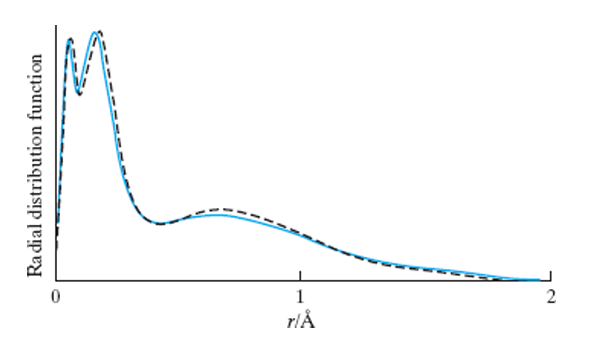
\includegraphics[width=0.65\textwidth]{Figures/11.1.png}
        \caption{
            \centering
            \parbox{0.6\linewidth}{
                \noindent
                \ce{Ar} 中径向分布函数与 $r$ 的函数关系。虚线是 Hartree–Fock 计算的结果。实线是电子衍射数据的结果。\\
                \small [Reprinted figure with permission from L.S. Bartell and L. O. Brockway, Physical Review Series II, Vol 90, 833, 1953. Copyright 1953 by the American Physical Society.]
            }
        }
        \label{fig:11.1}
    \end{figure}

    准确表示一个多电子原子轨道(AO)需要多个Slater型轨道的线性组合。对于粗略计算,使用简单的近似值来表示AO会更方便。我们可以使用具有有效核电荷的类氢轨道,但Slater提出了一种更简单的方法:用形式为(\ref{eq:11.14})的单一函数来近似AO,其中轨道指数$\zeta$取为
    \begin{equation}
        \zeta = \left(Z - s\right) / n
        \label{eq:11.15}
    \end{equation}
    其中$Z$为原子序数,$n$为轨道总量子数,$s$为屏蔽常数,可通过一组规则求得(见问题15.62)。Slater轨道用$r$的单次幂替换类氢轨道中$r$的多项式。因此,单个Slater轨道不具备正确的径向节点数,无法很好地表示轨道的内层部分。

    对多电子原子进行 Hartree–Fock SCF 计算(calculation)需要大量计算(computation)。在 20 世纪 30 年代,电子计算机尚未出现,Hartree 进行了多次 SCF 计算。幸运的是,Hartree 的父亲是一位退休工程师,他喜欢数字计算,并帮助了儿子。如今,计算机已经取代了 Hartree 的父亲。

\section{轨道和元素周期表}
\label{sec:11.2 Orbitals and the Periodic Table}














\section{电子相关}
\label{sec:11.3 Electron Correlation}

\section{角动量的叠加}
\label{sec:11.4 Addition of Angular Momenta}

\section{多电子原子的角动量}
\label{sec:11.5 Angular momentum in Many-Electron Atoms}

\section{自旋-轨道耦合}
\label{sec:11.6 Spin-Orbit Interaction}

\section{原子哈密顿算符}
\label{sec:11.7 The Atomic Hamiltonian}

\section{Condon-Slater规则}
\label{sec:11.8 The Condon-Slater Rules}

\section*{总结}

\section*{习题}

	
	% ===== CHAPTER 12 =====
\chapter{分子对称性}
\label{chap:12}
\section{对称元素和对称操作}
\label{sec:12.1 Symmetry Elements and Symmetry Operations}

\section{分子点群}
\label{sec:12.2 Molecular Point Groups}

\section*{总结}

\section*{习题}
	
	% ===== CHAPTER 13 =====
\chapter{双原子分子的电子结构}
\label{chap:13}
\section{Born-Oppenheimer近似}
\label{sec:13.1 The Born-Oppenheimer Approximation}

\section{双原子分子核的运动}
\label{sec:13.2 Nuclear Motion in Diatomic Molecules}

\section{原子单位制}
\label{sec:13.3 Atomic Units}

\section{氢分子离子}
\label{sec:13.4 The Hydrogen Molecular Ion}

\section{\ce{H^2+}离子基态的近似解}
\label{sec:13.5 Approximate Treatments of the H2 Ground Electronic State}

\section{\ce{H^2+}离子激发态的分子轨道}
\label{sec:13.6 Molecular Orbitals for H2 Excited States}

\section{同核双原子分子的分子轨道构型}
\label{sec:13.7 MO Configurations for Homonuclear Diatomic Molecules}

\section{双原子分子的分子光谱项}
\label{sec:13.8 Electronic Terms of Diatomic Molecules}

\section{氢分子}
\label{sec:13.9 The Hydrogen Molecule}

\section{价键理论求解\ce{H2}}
\label{sec:13.10 The Valence-Bond Treatment of H2}

\section{分子轨道理论和价键理论的比较}
\label{sec:13.11 Comparison of the MO and VB Theories}

\section{同核双原子分子的分子轨道理论和价键理论波函数}
\label{sec:13.12 MO and VB Wave Functions for Homonuclear Diatomic Molecules}

\section{\ce{H2}分子的激发态}
\label{sec:13.13 Excited States of H2}

\section{双原子分子的自洽场方法波函数}
\label{sec:13.14 SCF Wave Functions for Diatomic Molecules}

\section{分子轨道理论处理异核双原子分子}
\label{sec:13.15 MO Treatment of Heteronuclear Diatomic Molecules}

\section{价键理论处理异核双原子分子}
\label{sec:13.16 VB Treatment of Heteronuclear Diatomic Molecules}

\section{价电子近似}
\label{sec:13.17 The Valence-Electron Approximation}

\section*{总结}

\section*{习题}
	
	% ===== CHAPTER 14 =====
\chapter{分子量子力学理论}
\section{电子概率密度}

\section{偶极矩}

\section{分子的Hartree-Fork方法}

\section{Virial理论}

\section{Virial理论和化学键}

\section{Hellmann-Feynman理论}

\section{静电力定理}

\section*{总结}

\section*{习题}
	
	% ===== CHAPTER 15 =====
\chapter{分子的电子结构}
\label{chap:15}
\section{从头计算、密度泛函、半经验和分子力学方法}
\label{sec:15.1 Ab Initio, Density-Functional, Semiempirical and Molecular-Mechanics Methods}

\section{多原子分子的分子光谱项}
\label{sec:15.2 Electronic Terms of Polyatomic Molecules}

\section{自洽场方法、分子轨道理论求解多原子分子}
\label{sec:15.3 The SCF MO Treatment of Polyatomic Molecules}

\section{基函数}
\label{sec:15.4 Basis Functions}

\section{自洽场方法、分子轨道理论求解H$_2$O分子}
\label{sec:15.5 The SCF MO Treatment of the H$_2$O}

\section{布居分析和键级}
\label{sec:15.6 Population Analysis and Bond Orders}

\section{分子静电势、分子表面和原子电荷}
\label{sec:15.7 The Molecular Electrostatic Potential, Molecular Surfaces, and Atomic Charges}

\section{定域分子轨道}
\label{sec:15.8 Localized Molecular Orbitals}

\section{自洽场方法、分子轨道理论求解甲烷、乙烷和乙烯}
\label{sec:15.9 The SCF MO Treatment of Methane, Ethane, and Ethylene}

\section{分子结构学}
\label{sec:15.10 Molecular Geometry}

\section{构象搜寻}
\label{sec:15.11 Conformational Searching}

\section{分子振动频率}
\label{sec:15.12 Molecular Vibration Frequencies}

\section{热力学定律}
\label{sec:15.13 Thermodynamic Properties}

\section{从头计算方法的量子化学程序}
\label{sec:15.14 Ab Initio Quantum Chemistry Programs}

\section{进行从头计算}
\label{sec:15.15 Performing Ab Initio Calculations}

\section{快速Hartree-Fock计算方法}
\label{sec:15.16 Speeding Up Hartree-Fock Methods}

\section{溶剂效应}
\label{sec:15.17 Solvent Effects}

\section*{习题}
	
	% ===== CHAPTER 16 =====
\chapter{电子关联方法}
\label{chap:16}
\section{关联能}
\label{sec:16.1 Correlation Energy}

\section{组态相互作用}
\label{sec:16.2 Configuration Interaction}

\section{多体微扰理论}
\label{sec:16.3 MP Perturbation Theory}

\section{耦合簇方法}
\label{sec:16.4 The Coupled-Cluster Method}

\section{密度泛函理论}
\label{sec:16.5 Density-Functional Theory}

\section{能量计算的复合方法}
\label{sec:16.6 Composite Methods for Energy Calculations}

\section{扩散量子Monte Carlo法}
\label{sec:16.7 The Diffusion Quantum Monte Carlo Method}

\section{非共价相互作用}
\label{sec:16.8 Noncovalent Interactions}

\section{NMR屏蔽常数}
\label{sec:16.9 NMR Shielding Constants}

\section{碎裂法}
\label{sec:16.10 Fragmentation Methods}

\section{相对论效应}
\label{sec:16.11 Relativistic Effects}

\section{价键理论求解多原子分子}
\label{sec:16.12 Valence Bond Treatmen of Polyatomic Molecules}

\section{GVB(广义价键波函数)、VBSCF(价键自洽场)、BOVB(呼吸轨道价键)方法}
\label{sec:16.13 The GVB, VBSCF, and BOVB methods}

\section{化学反应}
\label{sec:16.14 Chemical Reactions}

\section*{习题}

	
	% ===== CHAPTER 17 =====
\chapter{半经验和分子力学方法求解分子}
\label{chap:17}
\section{半经验分子轨道求解平面共轭分子}
\label{sec:17.1 Semiempirical MO Treatments of Planar Conjugated Molecules}

\section{Hückel分子轨道理论}
\label{sec:17.2 The Hückel MO Method}

\section{PPP方法}
\label{sec:17.3 The PPP Method}

\section{一般的半经验分子轨道和密度泛函方法}
\label{sec:17.4 General Semiempirical MO and DFT Methods}

\section{分子力学方法}
\label{sec:17.5 The Molecular-Mechanics Method}

\section{经验和半经验方法处理溶剂效应}
\label{sec:17.6 Empirical and Semiempirical Treatments of Treating Solvent Effects}

\section{化学反应}
\label{sec:17.7 Chemical Reactions}

\section{量子化学的未来}
\label{sec:17.8 The Future of Quantum Chemistry}
	20 世纪 50 年代,人们普遍认为,除了非常小的分子之外,对所有分子性质进行有意义的从头计算法是不可能的。在这一时期撰写的量子化学书籍中,有这样的表述:“我们永远无法指望(对有机化合物)进行令人满意的从头计算法”,“对于比氢分子离子更复杂的系统,从一开始就放弃获得薛定谔方程精确解的尝试是明智的”。1959 年,Mulliken 和 Roothaan 发现了多原子分子量子力学精确计算的 “瓶颈”,即评估多中心积分的困难。现在,这一瓶颈已被消除。\\
	\indent 对中等尺寸分子进行 Hartree-Fork 从头计算法和几何优化已成为常规工作,并可采用计算效率较高的方法(如 DFT、MP2 和 SCS-MP2)将电子相关性包括在内。各种量子力学方法和基集的可靠程度已通过大量计算得到证实。可以进行精确从头计算法或密度泛函计算的分子大小受到现有电子计算机的速度和存储容量的限制。随着更大、更快计算机的开发,处理更大的分子将变得可行。\\
	\indent 近年来,量子化学取得了长足进步,量子力学计算已成为帮助解决各种实际化学问 题的重要工具。多年前,有关分子的量子力学计算主要局限于理论化学家阅读的期刊,而现在,这类计算经常出现在各种化学家阅读的期刊上,如《\textit{美国化学会志}》。量子化学正被应用于溶液中离子的水合、表面催化、反应中间产物的结构和能量、生物分子的构象以及酶催化反应的研究等问题。在许多情况下,理论计算可能无法给出明确的答案,但它们往往足以让理论与实验进行富有成效的互动。此外,伍德沃德-霍夫曼规则等定性概念也为化学反应过程和化学键的研究提供了重要启示。\\
	\indent 1998 年诺贝尔化学奖由沃尔特·科恩(Walter Kohn)(密度函数理论的开发者之一)和约翰·波普尔(John A. Pople)(高斯系列程序和广泛使用的高斯基集、PPP方法、CNDO 和 INDO 方法的开发者之一,以及最早将 MP 和 CC 方法应用于分子计算的人之一)分享。诺贝尔奖委员会指出:计算量子化学正在 “彻底改变整个化学”。

\section*{习题}


	
	% ===== APPENDIX =====

	\appendix
	
	% ===== APPENDIX =====
\chapter{附录}
\section{Complex Numbers}
A complex number $z = x + iy$ can be expressed as:
\begin{equation}
	z = re^{i\theta}, \quad r = \sqrt{x^2 + y^2}, \quad \theta = \tan^{-1}(y/x)
\end{equation}

\section{Calculus Formulas}
Key differentiation and integration formulas:
\begin{align}
	\dv{x}(e^{ax}) &= ae^{ax} \\
	\int \sin(ax) \dd{x} &= -\frac{1}{a} \cos(ax) + C
\end{align}
	
	% ===== BIBLIOGRAPHY =====
	
	% ===== BIBLIOGRAPHY =====
\chapter*{参考文献}
\begin{thebibliography}{9}
	\bibitem{levine} 
	Levine, I. N. (2014). \emph{Quantum Chemistry} (7th ed.). Pearson.
\end{thebibliography}
	
	% ===== ANSWERS TO SELECTED PROBLEMS =====
	
	% ===== ANSWERS TO SELECTED PROBLEMS =====
\chapter{部分习题答案}


	
	% ===== INDEX =====
	
	% ===== INDEX =====
\chapter{索引}
	
\end{document}